%% NYU PhD thesis format. Created by José Koiller 2007--2008.

%% Use the first of the following lines during production to
%% easily spot "overfull boxes" in the output. Use the second
%% line for the final version.
%\documentclass[12pt,draft,letterpaper]{report}
\documentclass[12pt,letterpaper]{report}

%% Replace the title, name, advisor name, graduation date and dedication below with
%% your own. Graduation months must be January, May or September.
\newcommand{\thesistitle}{Dynamical inference in the Milky Way}
\newcommand{\thesisauthor}{Jo~Bovy}
\newcommand{\thesisadvisor}{Professor David~W.~Hogg}
\newcommand{\graddate}{May 2011}
%% If you do not want a dedication, scroll down and comment out
%% the appropriate lines in this file.
%\newcommand{\thesisdedication}{To my dog Weierstra\ss, with affection.}

%% The following makes chapters and sections, but not subsections,
%% appear in the TOC (table of contents). Increase to 2 or 3 to
%% make subsections or subsubsections appear, respectively. It seems
%% to be usual to use the "1" setting, however.
\setcounter{tocdepth}{1}

%% Sectional units up to subsubsections are numbered. To number
%% subsections, but not subsubsections, decrease this counter to 2.
\setcounter{secnumdepth}{3}

%% Page layout (customized to letter paper and NYU requirements):
\setlength{\oddsidemargin}{.6in}
\setlength{\textwidth}{5.8in}
\setlength{\topmargin}{.1in}
\setlength{\headheight}{0in}
\setlength{\headsep}{0in}
\setlength{\textheight}{8.3in}
\setlength{\footskip}{.5in}

%% Use the following commands, if desired, during production.
%% Comment them out for final version.
%\usepackage{layout} % defines the \layout command, see below
%\setlength{\hoffset}{-.75in} % creates a large right margin for notes and \showlabels

%% Controls spacing between lines (\doublespacing, \onehalfspacing, etc.):
\usepackage{setspace}

%% Use the line below for official NYU version, which requires
%% double line spacing. For all other uses, this is unnecessary,
%% so the line can be commented out.
%\doublespacing % requires package setspace, invoked above

%% Each of the following lines defines the \com command, which produces
%% a comment (notes for yourself, for instance) in the output file.
%% Example:    \com{this will appear as a comment in the output}
%% Choose (uncomment) only one of the three forms:
%\newcommand{\com}[1]{[/// {#1} ///]}       % between [/// and ///].
\newcommand{\com}[1]{\marginpar{\tiny #1}} % as (tiny) margin notes
%\newcommand{\com}[1]{}                     % suppress all comments.

%% This inputs your auxiliary file with \usepackage's and \newcommand's:
%% It is assumed that that file is called "definitions.tex".
% Graphics:
\usepackage[final]{graphicx}
%\usepackage{graphicx} % use this line instead of the above to suppress graphics in draft copies
%\usepackage{graphpap} % \defines the \graphpaper command

%%BIBSTYLE
\usepackage[authoryear]{natbib}
\bibpunct{(}{)}{;}{a}{}{,}

% Indent first line of each section:
\usepackage{indentfirst}

% Fonts and symbols:
\usepackage{amsfonts,amssymb,amsmath}

%% others
\usepackage{url}
\usepackage{aas_macros}
\usepackage{deluxetable}

%%newcommands
%%Latin
\newcommand{\etal}{et~al.}
\newcommand{\eg}{e.g.}
\newcommand{\ie}{i.e.}

%%Figures etc
\newcommand{\figurenames}{\figurename s}
\newcommand{\sectionname}{\S}
\newcommand{\eqnname}{equation}


%%Solar system paper
\newcommand{\unit}[1]{\mathrm{#1}}
\newcommand{\AU}{\unit{AU}}
\newcommand{\unitday}{\unit{d}}
\newcommand{\yr}{\unit{yr}}
\newcommand{\satellite}[1]{\textsl{#1}}
\newcommand{\Gaia}{\satellite{Gaia}}
\newcommand{\KS}{K--S}
\newcommand{\tvector}[1]{\boldsymbol{\vec{#1}}}
\newcommand{\vx}{\tvector{x}}
\newcommand{\vv}{\tvector{v}}
\newcommand{\vxi}{\tvector{x}_i}
\newcommand{\vvi}{\tvector{v}_i}
\newcommand{\va}{\tvector{a}}
\newcommand{\vI}{\tvector{I}}
\newcommand{\vphi}{\tvector{\phi}}
\newcommand{\tuvector}[1]{\boldsymbol{\hat{#1}}}
\newcommand{\rhat}{\tuvector{r}}
\newcommand{\mvector}[1]{\boldsymbol{{#1}}}
\newcommand{\mvtheta}{\mvector{\theta}}
\newcommand{\mvthetae}{\mvector{\theta}_e}
\newcommand{\mvthetaepsilon}{\mvector{\theta}_{\epsilon}}
\newcommand{\mvomega}{\mvector{\omega}}
\newcommand{\mvomegahatk}{\mvector{\hat{\omega}}_k}
\newcommand{\mvDelta}{\mvector{\Delta}}
\newcommand{\dd}{\mathrm{d}}
\newcommand{\setofxv}{\{\vx_i,\vv_i\}}
\newcommand{\setofrv}{\{r_i,v_{r,i}\}}
\newcommand{\ueff}{u_{\mathrm{eff}}}
\newcommand{\rperi}{r_{\mathrm{peri}}}
\newcommand{\rap}{r_{\mathrm{ap}}}
\renewcommand{\angle}{\phi_r}
\newcommand{\anglei}{\phi_{r,i}}
\newcommand{\ff}{f_{\mvtheta}}
\newcommand{\fff}{\tilde{\ff}}
\newcommand{\lnepsilon}{\ln{\epsilon}}
\newcommand{\vperp}{j^2} % note strange definition
\newcommand{\vperpi}{j_i^2}
\newcommand{\gradient}{\mvector{\nabla}_{\!\!\mvomega}}
\newcommand{\wk}{\ensuremath{w_k}}
\newcommand{\nk}{\ensuremath{n_k}}



%%MASERS
\newcommand{\lsr}{LSR}
\newcommand{\vsunlsr}{\ensuremath{v_\odot}}
\newcommand{\vsunlsrx}{\ensuremath{v_{\odot,x}}}
\newcommand{\vsunlsry}{\ensuremath{v_{\odot,y}}}
\newcommand{\vsunlsrz}{\ensuremath{v_{\odot,z}}}
\newcommand{\vlsr}{\ensuremath{v_{\mbox{\footnotesize \lsr}}}}
\newcommand{\omegao}{\ensuremath{\Omega_0}}
\newcommand{\Ro}{\ensuremath{R_0}}
\newcommand{\zo}{\ensuremath{z_0}}
\renewcommand{\vec}[1]{\mathbf{#1}} % boldface for vectors
\newcommand{\mm}{\ensuremath{\vec{m}}}
\newcommand{\zerovector}{\ensuremath{\vec{0}}}
\newcommand{\masermean}{\ensuremath{\overline{\vv}}}
\newcommand{\samplemean}{\ensuremath{\overline{\tvector{\mu}}}}
\newcommand{\mmR}{\ensuremath{\overline{v}_R}}
\newcommand{\mmphi}{\ensuremath{\overline{v}_\phi}}
\newcommand{\mmz}{\ensuremath{\overline{v}_z}}
\newcommand{\vvpec}{\ensuremath{\vv_{\mbox{{\footnotesize pec}}}}}
\newcommand{\vpec}{\ensuremath{v_{\mbox{{\footnotesize pec}}}}}
\newcommand{\vvmaser}{\ensuremath{\vv_{\mbox{{\footnotesize maser}}}}}
\newcommand{\eeR}{\ensuremath{\vec{e}_{R}}}
\newcommand{\eephi}{\ensuremath{\vec{e}_{\phi}}}
\newcommand{\eez}{\ensuremath{\vec{e}_{z}}}
\newcommand{\vvRi}{\ensuremath{\vpec_{R,i}}}
\newcommand{\vvphii}{\ensuremath{\vpec_{\phi,i}}}
\newcommand{\vvzi}{\ensuremath{\vpec_{z,i}}}
\newcommand{\vvpeci}{\ensuremath{\vvpec_i}}
\newcommand{\ten}[1]{\mathbf{#1}} % boldface for tensors
\newcommand{\RR}{\ten{R}}
\newcommand{\VV}{\ten{V}}
\newcommand{\WW}{\ten{W}}
\newcommand{\II}{\ten{I}}
\newcommand{\TT}{\ten{T}}
\newcommand{\AAA}{\ten{A}}
\newcommand{\maserdisp}{\ensuremath{\mbox{\boldmath$\sigma$}}}
\newcommand{\vgalx}{\ensuremath{\tilde{v}_x}}
\newcommand{\vgaly}{\ensuremath{\tilde{v}_y}}
\newcommand{\vgalz}{\ensuremath{\tilde{v}_z}}
\newcommand{\normal}{\ensuremath{\mathcal{N}}}
\newcommand{\wishart}{\ensuremath{\mathcal{W}}}
\newcommand{\gammadist}{\ensuremath{\mathcal{G}}}
\newcommand{\trace}{\mbox{Trace}}
\newcommand{\T}{^{\scriptscriptstyle \top}}   % transpose
\newcommand{\offsets}{\ensuremath{\Delta\vx_i, \Delta \vv_i}}
\newcommand{\alloffsets}{\ensuremath{\{\offsets\}}}
\newcommand{\pmsgra}{\ensuremath{\mu_{\mbox{{\footnotesize Sgr A$^*$}}}}}
\newcommand{\vres}{\ensuremath{\tvector{v}_{\mbox{{\footnotesize res}}}}}
\newcommand{\vresi}{\ensuremath{\tvector{v}_{\mbox{{\footnotesize res}}, i}}}
\newcommand{\vgal}{\ensuremath{\tvector{v}_{\mbox{{\footnotesize Gal}}}}}
\newcommand{\vgali}{\ensuremath{\tvector{v}_{\mbox{{\footnotesize Gal}}, i}}}

\newcommand{\vlba}{VLBA}
\newcommand{\vlbi}{VLBI}
\newcommand{\vera}{VERA}
\newcommand{\reid}{R09}
\newcommand{\vc}{V_c}
\newcommand{\mw}{MW}

\newcommand{\ra}{\ensuremath{\alpha}}
\newcommand{\dec}{\ensuremath{\delta}}
\newcommand{\pmra}{\ensuremath{\mu_{\ra}}}
\newcommand{\pmdec}{\ensuremath{\mu_{\dec}}}
\newcommand{\eqx}{\ensuremath{x_{\textnormal{eq}}}}
\newcommand{\eqy}{\ensuremath{y_{\textnormal{eq}}}}
\newcommand{\eqz}{\ensuremath{z_{\textnormal{eq}}}}
\newcommand{\gall}{{\it l}}
\newcommand{\galb}{{\it b}}
\newcommand{\pmll}{\ensuremath{\mu_\gall}}
\newcommand{\pmbb}{\ensuremath{\mu_\galb}}
\newcommand{\galx}{\ensuremath{x}}
\newcommand{\galy}{\ensuremath{y}}
\newcommand{\galz}{\ensuremath{z}}
\newcommand{\galU}{\ensuremath{U}}
\newcommand{\galV}{\ensuremath{V}}
\newcommand{\galW}{\ensuremath{W}}
\newcommand{\parallax}{\ensuremath{\varpi}}
\newcommand{\radialdist}{\ensuremath{d}}
\newcommand{\vrr}{\ensuremath{v_r}}
\newcommand{\vll}{\ensuremath{v_\gall}}
\newcommand{\vbb}{\ensuremath{v_\galb}}
\newcommand{\vernal}{\ensuremath{\Upsilon}}
\newcommand{\ngp}{\textnormal{NGP}}
\newcommand{\ngpg}{\textnormal{G}}
\newcommand{\ncp}{\textnormal{NCP}}
\newcommand{\ncpp}{\textnormal{P}}
\newcommand{\gc}{\textnormal{GC}}
\newcommand{\gcc}{\textnormal{C}}
\newcommand{\rangp}{\ensuremath{\ra_\ngp}}
\newcommand{\decngp}{\ensuremath{\dec_\ngp}}
\newcommand{\ragc}{\ensuremath{\ra_\gc}}
\newcommand{\decgc}{\ensuremath{\dec_\gc}}
\newcommand{\degree}{^{\circ}}
\newcommand{\matrixleft}{\left[}
\newcommand{\matrixright}{\right]}
\newcommand{\arcsecs}{\textnormal{as}}

%%HERCULES
\newcommand{\apogee}{APOGEE}
\newcommand{\hermes}{HERMES}
\newcommand{\hipparcos}{\emph{Hipparcos}}
\newcommand{\vR}{\ensuremath{v_R}}
\newcommand{\vphihercules}{\ensuremath{v_{\phi}}}
\newcommand{\vo}{\ensuremath{v_0}}
\newcommand{\ro}{\Ro}
\newcommand{\Ab}{\ensuremath{A_b}}
\newcommand{\Rb}{\ensuremath{R_b}}
\newcommand{\Omegab}{\ensuremath{\Omega_b}}
\newcommand{\fdehnen}{\ensuremath{f_{\text{Dehnen}}}}
\newcommand{\sigmaR}{\ensuremath{\sigma_R}}
\newcommand{\rE}{\ensuremath{R_e}}
\newcommand{\Lc}{\ensuremath{L_c}}
\newcommand{\Rs}{\ensuremath{R_s}}
\newcommand{\Rsigma}{\ensuremath{R_{\sigma}}}
\newcommand{\Rolr}{\ensuremath{R_{\text{OLR}}}}


%% Cross-referencing utilities. Use one or the other--whichever you prefer--
%% but comment out both lines for final version.
%\usepackage{showlabels}
%\usepackage{showkeys}


\begin{document}
%% Produces a test "layout" page, for "debugging" purposes only.
%% Comment out for final version.
%\layout % requires package layout (see above, on this same file)

%%%%%% Title page %%%%%%%%%%%
%% Sets page numbering to "roman style" i, ii, iii, iv, etc:
\pagenumbering{roman}
%
%% No numbering in the title page:
\thispagestyle{empty}
\setlength{\topmargin}{.6in}
%
\begin{center}
  {\large\textbf{\thesistitle}}
  \vspace{.7in}

  by
  \vspace{.7in}

  \thesisauthor
  \vspace{1.7in}

\begin{doublespace}
  A dissertation submitted in partial fulfillment\\
  of the requirements for the degree of\\
  Doctor of Philosophy\\
  Department of Physics\\
  New York University\\
  \graddate
\end{doublespace}
\end{center}
\vspace{1.4in}

\noindent\makebox[\textwidth]{\hfill\makebox[2.5in]{\hrulefill}}\\
\makebox[\textwidth]{\hfill\makebox[2.5in]{\hfill\thesisadvisor\hfill}}
\newpage
%%%%%%%%%%%%% Blank page %%%%%%%%%%%%%%%%%%
\thispagestyle{empty}
\vspace*{0in}
\setlength{\topmargin}{.1in}
\newpage

%%%%%%%%%%%%%% Frontispiece %%%%%%%%%%%%%%%%%
%% Comment out the following lines if you do not want a frontispiece
%% this to anyone...
\thispagestyle{empty}
\vspace*{\fill}
\begin{center}
  \emph{``Die Welt ist alles, was der Fall ist.''}\\
— Ludwig Wittgenstein (Tractatus Logico-Philosophicus)
\end{center}
\vfill
\newpage
%%%%%%%%%%%%%% Dedication %%%%%%%%%%%%%%%%%
%% Comment out the following lines if you do not want to dedicate
%% this to anyone...
%\vspace*{\fill}
%\begin{center}
%  \thesisdedication\addcontentsline{toc}{section}{Dedication}
%\end{center}
%\vfill
%\newpage
%%%%%%%%%%%%%% Acknowledgements %%%%%%%%%%%%
%% Comment out the following lines if you do not want to acknowledge
%% anyone's help...
\section*{Acknowledgements}\addcontentsline{toc}{section}{Acknowledgements}


Hogg

Fr{\'e}d{\'e}ric Arenou, Michael Aumer, Coryn Bailer-Jones, James
Binney, Michael Blanton, Anthony Brown, Daniela Carollo, Ilias Cholis,
Kyle Cranmer, Walter Dehnen, Mulin Ding, Glennys Farrar, Ken Freeman,
Stefan Gillessen, Andrei Gruzinov, Kathryn Johnston, Joe Hennawi, Matt
Kleban, Dustin Lang, Floor van Leeuwen, Yuri Levin, Stephen Levine,
Tom Loredo, Dmitry Malyshev, Phil Marshall, Surhud More, John
Moustakas, Iain Murray, Adam Myers, Bill Press, Mark Reid, Hans-Walter
Rix, Sam Roweis, Erin Sheldon, Michael Strauss, Scott Tremaine, Glenn
van de Ven, David Weinberg, Neal Weiner, and a few anonymous referees.

Funding agencies: the National Aeronautics and Space Administration
(ADP grant NNX08AJ48G) and the National Science Foundation (grant
AST-0908357). Partial support from the Max-Planck-Institut f\"ur
Astronomie, a New York University Horizon fellowship, and a Horizon
Dissertation writing fellowship. I would also like to acknowledge the
hospitality of The Max-Planck-Institut f\"ur Astronomie and the
Lorentz Center in Leiden.

Software: the HORIZONS System provided by the Solar System Dynamics
Group of the Jet Propulsion Laboratory, the NASA Astrophysics Data
System, and the open-source Python modules scipy, numpy, and
matplotlib.




\newpage
%%%% Abstract %%%%%%%%%%%%%%%%%%
\section*{Abstract}\addcontentsline{toc}{section}{Abstract}
Current and future surveys of the Galaxy contain a wealth of
information about the structure and evolution of the Galactic disk and
halo. Teasing out this information is complicated by measurement
uncertainties, missing data, and sparse sampling. I develop and
describe several applications of generative modeling--—creating an
approximate description of the probability of the data given the
physical parameters of the system--—to deal with these issues.

I develop a method for inferring the Galactic potential from
individual observations of stellar kinematics such as will be
furnished by the upcoming \Gaia\ space astrometry mission. This method
takes uncertainties in our knowledge of the distribution function of
stellar tracers into account through marginalization. I demonstrate
the method by inferring the force law in the Solar System from
observations of the positions and velocities of the eight planets at a
single epoch. I apply a similar method to derive the Milky Way's
circular velocity from observations of maser kinematics.

I infer the velocity distribution of nearby stars from
\hipparcos\ data, which only consist of tangential velocities, by
forward modeling the underlying distribution with a flexible
multi-Gaussian model. I characterize the contribution of several
``moving groups''---overdensities of co-moving stars---to the full
distribution. By studying the properties of stars in these moving
groups, I show that they do not form a single-burst population and
that they are most likely due to transient non-axisymmetric features
of the disk, such as transient spiral structure. By forward modeling
one such scenario, I show how the Hercules moving group can be traced
around the Galaxy by future surveys, which would confirm that the
Milky Way bar's outer Lindblad resonance lies near the Solar radius.

\newpage
%%%% Table of Contents %%%%%%%%%%%%
\tableofcontents

%%%%% List of Figures %%%%%%%%%%%%%
%% Comment out the following two lines if your thesis does not
%% contain any figures. The list of figures contains only
%% those figures included withing the "figure" environment.
\listoffigures\addcontentsline{toc}{section}{List of Figures}
\newpage

%%%%% List of Tables %%%%%%%%%%%%%
%% Comment out the following two lines if your thesis does not
%% contain any tables. The list of tables contains only
%% those tables included withing the "table" environment.
\listoftables\addcontentsline{toc}{section}{List of Tables}
\newpage

%%%%% Body of thesis starts %%%%%%%%%%%%
\pagenumbering{arabic} % switches page numbering to arabic: 1, 2, 3, etc.
%% Introduction. If your thesis has no introduction, or chapter 1 is
%% meant to be the introduction, then comment out the lines below.
\chapter*{Introduction}\addcontentsline{toc}{chapter}{Introduction}
In the current understanding of the formation of structure in the
Universe the initial tiny density fluctuations are generated during an
inflationary epoch. The dominant mass component---the dark
matter---starts to cluster under the influence of gravity after the
dark matter decouples from the other constituents of the early
Universe, while the ordinary matter of atoms and everyday life remains
coupled to radiation until about 300,000 years after the Big
Bang. When the temperature of the Universe drops below about 3,000 K,
ordinary matter decouples from radiation and falls into the potential
wells created by dark-matter clustering. Ordinary matter is
predominantly found as neutral hydrogen at this stage and this gas
settles at high density at the bottoms of the dark matter
potentials. Stars and later galaxies form in these high density regions.

The current paradigm has been successful in explaining the large-scale
properties of the Universe, especially the close-to-linear regime of
the Cosmic Microwave Background, formed at the epoch of
ordinary-matter--radiation decoupling, and the largest ($> 100 Mpc$
scales in the nearby Universe, where the non-linear influence of
gravity does not play a large role. However, the formation and
evolution of individual galaxies remains to be understood. This is
obvious from the many classes of galaxies and other objects identified
locally (\eg, the Hubble sequence, dwarf Spheroidal galaxies, dwarf
irregular galaxies, etc.) and at higher redshift (\eg, Ultraluminous
infrared galaxies, sub-millimeter galaxies, Lyman-limit systems,
Damped Lyman-$\alpha$ absorbers, MgII absorbers, etc.). How all these
systems form and relate to one another is yet to be explained. 

Since most of Galactic and extra-galactic astronomy is limited to
snapshots at a particular time, one can study the formation and
evolution of galaxies either by looking at galaxies at different
redshifts and interpreting these observations as different stages in
the evolution of present-day galaxies, or one can study galaxies
locally, where observations with much more detail are possible,
especially for the Milky Way and M31, and infer their formation and
evolution. These two approaches move in remarkable lockstep, as the
highest redshifts probed (BOVY: CHANGE) by current and planned surveys
are comparable to the times at which the lowest metallicity stars
currently studied in the Milky Way formed (BOVY: CITE
BLAND+FREEMAN). These approaches are therefore strongly
interrelated. This dissertation focuses on the latter approach.



Absence of major merger for MW (10 Gyr, redshift ?). 


It is known for certain that there is a large amount of dark mass
beyond the Sun’s position in the Milky Way. We expect there to be dark
matter in the inner region of the Galaxy as well. The determination of
the mass distribution in the inner Galaxy, and its decomposition into
the stellar and dark components, is made difficult by the ambiguity of
local stars as tracers of the mass distribution; certain distracting
disk dynamical features such as spiral arms; and our own (moving)
position in the middle of all of this.

While the Milky Way is interesting in its own right—--it is our home
in the Universe--—it is only one among thousands of galaxies in the
local Universe. Despite this, the Milky Way is one of the main sites
for studying structure formation in the Universe on small scales,
because of the amazing amount of detail possible in these
observations. For comparison, the apparent size of the Milky Way’s
nearest neighbor, the Andromeda galaxy, is only a few times that of
the full moon; other nearby galaxies are much farther away. Since we
have no reason to believe that the Milky Way is atypical in any
way—--we can detect many galaxies with similar features in the night
sky—the details of the Milky Way’s mass distribution and formation
history also provide a general understanding of how galaxies form.


Since stars move across the sky at a slow pace and because they orbit
the Galaxy on timescales measured in hundreds of millions of years, we
can hope at best to measure their positions and velocities at the
present time, while their accelerations are beyond our observational
reach. This poses a fundamental difficulty for interpreting the data
in terms of the mass distribution that guides them.  Newton’s second
law says that the acceleration of a star is directly set by the force
acting on it, while its velocity merely reflects the initial motion of
the object and not the underlying force. Thus, without the
accelerations of stars it seems that we cannot know the underlying
mass distribution. This problem and its resolution is discussed in
Chapter I.

To derive the mass distribution of the Milky Way from stellar motions,
we need to make additional assumptions about the kinematics of stars
that couple these motions to the mass distribution. One such
assumption is that the distribution of the stellar positions and
velocities is time-independent.  This seemingly simple assumption
provides the coupling between the underlying mass distribution and the
stellar kinematics. As an example, I show that we can determine the
force law in the Solar System from observations of the planets’
positions and velocities at one epoch. The nontrivial part of this toy
data set’s analysis is that one has to model the distribution of the
planets’ positions and velocities in a timeindependent manner while
not introducing extra assumptions. I achieve this by building a full
probabilistic model of the data that introduces extra degrees of
freedom describing the time-independent distribution of the positions
and velocities; these extra degrees of freedom can be integrated over
to obtain the final result for the force law in the Solar System which
is independent of the extra degrees of freedom.

Another application considers not observations of stars directly, but
the light of young stars, reprocessed and amplified by the molecular
gas clouds surrounding them. These masers—--lasers on a cosmic
scale—--can be seen to large distances, and their kinematics can be
measured by radio observatories much more precisely than is possible
for stars with optical telescopes. The current data set of 18 masers
contains much information about the disk’s structure, but the
interpretation of the data again depends on our assumptions about the
distribution of their positions and velocities. By inferring a simple
model in which the velocities of the masers are scattered around a
mean offset from the velocity associated with circular motion, we
obtain this circular velocity at the Sun’s position in the
Galaxy. This tells us directly about the Galaxy’s mass within the
Solar radius. This work has been published (Bovy et al. 2009,
Astrophys. J.  704, 1704). 

Chapter III concerns the available data on the motions of stars in the
Galactic disk. The Hipparcos satellite has accurately measured the
positions and motions of stars close to the Sun, which allows us to
look at their detailed properties. First I reconstruct the local
velocity distribution from these data. The result is complex which one
would not expect if the assumptions—axisymmetry and timeindependence
—introduced in the previous paragraphs were correct (this work has
been published: Bovy et al. 2009, Astrophys. J. 700, 1794). Looking at
the mixture of stars that make up the unexpected complexity, I find
that these stars have not formed together such that the complexity is
not due to a formation-history time-dependence and axisymmetry must be
broken. By considering how consistently we can measure the Sun’s
motion relative to the local circular velocity (measured in chapter
II)—--Assuming axisymmetry, this measurement is possible—--I find that
the disk is non-axisymmetric at the level of a few percent.

%% If your thesis has different "Parts", use commands such as the following:
%\part{First Part\label{part:one}}%
\newcounter{tableone}

\chapter[Dynamical inference from a kinematic snapshot: The force law in the Solar System]{Dynamical inference from a kinematic snapshot:\\
  The force law in the Solar System\protect\footnote{Iain~Murray, David~W.~Hogg}\label{chap:solarsystem}}

%\begin{abstract}
%If a dynamical system is long-lived and non-resonant (that is, if
%there is a set of tracers that have evolved independently through many
%orbital times), and if the system is observed at any non-special time,
%it is possible to infer the dynamical properties of the system (such
%as the gravitational force or acceleration law) from a snapshot of the
%positions and velocities of the tracer population at a single moment
%in time. In this paper we describe a general inference technique that
%solves this problem while allowing (1)~the unknown distribution
%function of the tracer population to be simultaneously inferred and
%marginalized over, and (2)~prior information about the gravitational
%field and distribution function to be taken into account. As an
%example, we consider the simplest problem of this kind: We infer the
%force law in the Solar System using only an instantaneous kinematic
%snapshot (valid at 2009 April 1.0) for the eight major planets. We
%consider purely radial acceleration laws of the form $a_r=
%-A\,[r/r_0]^{-\alpha}$, where $r$ is the distance from the Sun.  Using
%a probabilistic inference technique, we infer $1.989<\alpha<2.052$
%(95~percent interval), largely independent of any assumptions about
%the distribution of energies and eccentricities in the system beyond
%the assumption that the system is phase-mixed. Generalizations of the
%methods used here will permit, among other things, inference of
%Milky-Way dynamics from \Gaia-like observations.
%\end{abstract}

\section{Introduction}

The \Gaia~Satellite \citep{Perryman01a} will measure positions and
velocities for millions to billions of stars at varying precision.
One of the principal goals of this mission is to provide the data
necessary to infer the dynamical state of the Milky Way.  However,
there are issues in principle with inference of dynamics from a
\emph{snapshot} or instantaneous set of configuration and velocity
measurements: The instantaneous positions and velocities have no
\emph{necessary} relationship with the gravitational potential or
accelerations.  Indeed, despite a considerable literature \citep[for
  example,][]{Oort32, Schwarzschild79, Little87a, Binney94,
  Johnston99, roulette} there is no methodology for performing this
inference that naturally handles all of the issues, including finite
and non-trivial observational uncertainties or noise, missing data,
non-steady aspects of the mass distribution, and the (incredibly
likely) possibility that the potential is not (simply) integrable.
Robust inference may not even be \emph{possible} if the Milky Way has
significant time-dependence or is strongly chaotic or is far from
showing any simple symmetries (such as axisymmetry).

Certainly there is no hope for dynamical inference on the massive
scale required for the \Gaia\ data set if we can't perform it on much
simpler, much more symmetrical, much older (in a dynamical sense), and
much smaller (in a data sense) systems.  In what follows, we take one
of the simplest possible systems---the Solar System---and the smallest
possible data set---the positions and velocities of the major planets at a
moment in time---and perform a complete dynamical inference.  For a
test system we could also have chosen the black hole at the Galactic
Center, where similar considerations apply.  However, this system has
additional issues with ``missing data'' because not all six
phase-space coordinates are directly measurable for all stars.  The
Solar System truly is the simplest problem in this class.

Our inferential starting point is orbital roulette \citep{roulette}.
In this previous work, it was assumed that the orbital angles (in the
action-angle formalism) are uniformly distributed. Thus, dynamical
model parameters that correspond to orbital angles that suspiciously
lack diversity are rejected. More specifically, the method considers a
large range of possible dynamical model parameters, computes orbital
angles at every value of the parameters, and a distribution statistic
on those orbital angles. If the distribution statistic is designed to
monotonically increase with the diversity of the angles or the
flatness of the angle distribution, the ``best fit'' dynamical model
parameters are those that optimize the distribution statistic.  This
kind of approach is inherently frequentist: on many applications of
these procedures to independent datasets a confidence interval
captures the true dynamical parameters on a guaranteed fraction of
trials. However, for any given dataset the confidence interval
produced might not represent a credible set of parameters.

In what follows we cast the dynamical parameters estimation as a
probabilistic inference problem (a ``Bayesian'' approach). We adopt
the same core assumption as the roulette problem: we assume that the
orbital angles are uniformly distributed. However, in this framework,
we must also construct prior probability distribution functions for
the dynamical model parameters and conditional probabilities of the
data given the model to encode the assumptions of a long-lived and
bound Solar System.  These prior and conditional probability
distributions and the data create posterior probability distribution
functions for all the parameters. We use this new method to infer the
gravitational force law (radial dependence and amplitude).  What is
new here, in the context of Solar System dynamics, is that we perform
this inference with only a snapshot of the kinematic state, that is,
with only the positions and velocities of the planets at a
\emph{single instant of time.}

Of course the kinematic snapshot we employ is, in fact, a set of
initial conditions for a Solar System integration \citep{Giorgini96a}.
These initial conditions were determined not by a single measurement
at a single epoch, but are in fact the result of an optimization of a
Solar System integration to observed planetary positions over many
decades.  In the context of this paper---a demonstration of a
method---it is best to think of these ``data'' as ``simulated data''
useful for testing the method.  They just happen to be data that have
been simulated by the analog computer we know as the Solar System.

What is new here, in the context of dynamical inference, is that our
method is fully probabilistic or Bayesian.  This is important for
future problems, such as the \Gaia\ problem, or for inferring the mass
of the black hole at the center of the Milky Way, because in these
real data analysis problems, the data points come with non-trivial and
highly correlated observational uncertainties, and because entire
dimensions of phase space are missing or unobserved.  At the Galactic
Center, we do not know the radial distance to anything accurately, and
in the \Gaia\ data set many of the radial velocities will not be
measured.  The Bayesian framework handles these real-world data issues
very naturally, although in fact they are \emph{not} important in the
test problem we solve here.  Aside from these issues of principle, it
is also the case, as we will show, that the Bayesian method performs
extremely well.

Of course, a lot is known about the gravitational force law in the
Solar System, so we don't expect, at the outset, to be surprised by
our results.  The first force-law inference in the Solar System
\citep[][and also work by contemporaries, particularly Hooke, who may
  have priority]{Newton} made use of full orbit shape determination
\citep{Kepler}.  In this sense, Newton's problem---find the force law
(from among a small, discrete group of possible force laws) that leads
to elliptical orbits with the Sun at one focus---was much easier than
the problem we have set for ourselves.  Of course, along the way,
Newton had to develop for the first time the general principles of
kinematics and dynamics!

\section{Parameterized force law, or dynamical model}\label{sec:model}

We are going to assume spherical symmetry of the Solar System's force
law and gravitational potential, although nothing in the general
inference formalism that follows will require this.  Consider a radial
force law (really acceleration law) of the form
\begin{equation}
\va = -A\,\left[\frac{r}{r_0}\right]^{-\alpha}\,\rhat \quad,
\end{equation}
where $A$ is an amplitude, $r$ is the distance from the Sun, $r_0$ is
a distance scale (in this case we will use $r_0=1\,\AU$ so that $A$
can be thought of as the acceleration at the Earth's orbit), $\alpha$
parameterizes the radial dependence, and $\rhat$ is the radial
direction.  In this model, the list of free parameters is
\begin{equation}
\mvomega \equiv \{\ln A,\alpha\}\quad,
\end{equation}
where we have taken the logarithm of $A$ because in inference
problems, dimensioned parameters are usually best handled in the log
\citep{Jeffreys39a,Sivia06a}.

The potential $u$ (potential energy per unit planet mass), radial
effective potential $\ueff$, and binding
energy per unit mass $\epsilon\equiv -E/m$ are
\begin{equation}
u(r) = \frac{A\,r_0}{1-\alpha}\,\left[\frac{r}{r_0}\right]^{1-\alpha} \quad,
\end{equation}
\begin{equation}
\ueff(r) = u(r) + \frac{j^2}{2\,r^2} \quad,
\end{equation}
\begin{equation}
\epsilon = - \ueff - \frac{1}{2}\,v_r^2 \quad,
\end{equation}
where $j^2$ is the square of the magnitude of the planet's angular
momentum per unit mass (or $L^2/m^2$), and $v_r$ is the radial
component of the velocity (the component of $\vv$ parallel to
$\vxsolar$).  The perihelion and aphelion distances $\rperi$ and
$\rap$ are both found by setting $\epsilon=-\ueff$.  With these, we
can define a radial asymmetry $e$
\begin{equation}
e \equiv \frac{\rap - \rperi}{\rap + \rperi} \quad,
\end{equation}
where we have called this ``$e$'' because in the Kepler--Newton
$\alpha=2$ case it is the orbital eccentricity.  One way of thinking of
this radial asymmetry is that at any point in the space made up of the
dynamical parameters $\mvomega$ and the binding energy $\epsilon$,
the radial asymmetry $e$ is a dimensionless description of the
angular momentum magnitude.

Importantly for what follows, we can define a ``radial angle''
$\angle$ that increases linearly with time from perihelion passage
through next perihelion passage.  Any planet at radius $r$ on an orbit
with perihelion distance $\rperi$ and aphelion distance $\rap$ can be
assigned this angle $\angle$ by
\begin{equation}
\angle \equiv \left\{\begin{array}{cl}\displaystyle
  \pi\,\frac{t(r)-t(\rperi)}{t(\rap)-t(\rperi)} & \mbox{for $v_r > 0$}
  \\[2.5ex] \displaystyle
  \pi+\pi\,\frac{t(r)-t(\rap)}{t(\rperi)-t(\rap)} & \mbox{for $v_r < 0$}
\end{array}\right. \quad,
\end{equation}
where the first numerator is the time it takes to go from $\rperi$ to
$r$ outbound, the first denominator is the time it takes to go from
$\rperi$ to $\rap$ outbound, the second numerator and denominator are
the times inbound, and all time differences between two radii can be
computed numerically for general values of $\alpha$ by integrating the
inverse of the radial velocity between these radii. The first-order
form of this integral has an integrable singularity at the perihelion
and aphelion, which can be handled by an appropriate change of
variables \citep[\eg, ][]{Press07a}. A planet observed at a set of
random times spanning many orbits will be observed to have radial
angles $\angle$ drawn from a flat distribution in the range
$0<\angle<2\,\pi$.  This radial angle is one of the angles in the
action-angle formulation of the system, which is integrable for the
simple reason that it is spherically symmetric.

\section{Kinematic data}

In what follows, we are going to use and compare several methods for
inferring the force-law parameters $\mvomega$ (the amplitude $\ln A$
and radial exponent $\alpha$ of the spherical force law) from an
instantaneous snapshot of the positions and velocities of the eight
major planets.  This snapshot was taken from JPL's HORIZONS System
which provides highly accurate ephemerides for Solar System
objects\footnote{Available at \url{http://ssd.jpl.nasa.gov/?horizons}}
\citep{Giorgini96a}. It is an extrapolation (at the time of writing)
to 2009 April 1.0, approximately 400 years after the important
publication of Kepler (1609). This kinematic snapshot is given in
Table~\ref{table:eph}.

Since this snapshot is obtained by integrating the positions and
velocities of Solar System bodies, the accuracy is limited by (i) the
correctness of the dynamical model used, (ii) the numerical
integration of the equations of motion, and (iii) the accuracy to
which the initial conditions are known. It is generally believed that
the dynamical model used is correct and complete, and that the
numerical integration is sufficiently accurate. The main uncertainty
in the ephemerides is then that due to the uncertainty in the initial
conditions. The current set of initial conditions
\citep[DE405;][]{Standish98a} is a fit to a set of optical, radar, and
VLBI observations as well as to a set of spacecraft range and Doppler
points from various space missions. The uncertainties are the largest
for the outer planets, since the data for these are almost entirely
from optical observations (with the exception of Jupiter), and because
Neptune has not been observed over a full orbit since the start of
precise measurements. A comparison between the DE405 ephemerides and
more recent observations shows that the positions of the inner planets
are known to a fractional accuracy of approximately $10^{-8}$, while
those of the outer planets are known to a fractional accuracy of
$10^{-6}$ to $10^{-7}$ \citep{Standish04a}. Uncertainties in the
velocities are at the same fractional magnitude.

This kinematic snapshot is not, of course, a fair data set with which
to perform the inference below, for the main reason that the
``measured'' kinematic state of the Solar System is in fact the output
of fitting observations with a dynamical model that \emph{assumes}
$\alpha=2$.  For this reason, the data should be thought of as
``idealized'' or ``simulated data'' and the work must be considered a
test of the method rather than a definitive inference.

\section{Bound, virialized, and long-lived}

The virial theorem relates the time averages $\left<T\right>$ and
$\left<U\right>$ of a test particle's kinetic and potential energies
through
\begin{equation}\label{eq:virialtheorem}
\left<T\right> = \frac{1-\alpha}{2}\,\left<U\right> \quad,
\end{equation}
where $\alpha$ is the exponent in the radial force law.  Given that a
planet's potential energy is a function of the dynamical parameters
$\mvomega$, while its kinetic energy is not, the virial relation for
each planet becomes a one-dimensional locus in the $\mvomega$ space.
Using kinetic and potential energies computed from the observations as
a proxy for the time-averaged energies, these loci are shown in
\figurenames~\ref{fig:virial_main} and \ref{fig:virial_zoom}.  The
fact that all eight lines cross near a single point in the space is
encouraging that the system is virialized (as we expect) and that the
inference will work. That the eight lines so nearly intersect in a
single point is because, in fact, many of the planets are on circular
orbits; the probabilistic method developed in this paper does not
assume this, but it does retain the precision that is possible because
of this situation.

Also shown in \figurenames~\ref{fig:virial_main} and
\ref{fig:virial_zoom} is the region of parameter space in which one or
more of the planets is unbound because $T>U$ or, equivalently,
$\epsilon < 0$.  In what follows, we will assign vanishing probability
to regions of parameter space in which one or more planets is
unbound. However, as we will see, this does not affect any of our
conclusions. Also shown in \figurename~\ref{fig:virial_main} is the
region of parameter space in which one or more of the planets has
$\rperi<R_\odot$, where $R_\odot$ is the radius of the Sun.  This part
of parameter space ought also to be excluded, although in practice
this is not necessary for any of what follows.

In preparation for what follows, we pre-compute all of the planet
radial angles $\anglei$---given their positions $\vxsolar_i$ and
velocities $\vv_i$---as a function of the dynamical parameters.  These
angles are shown in \figurename~\ref{fig:anglesPlanets}.

\section{Frequentist orbital roulette}\label{sec:freq}

In orbital roulette \citep{roulette}, the idea is to compute, for each
point $\mvomega$ in parameter space, the $N$ radial angles $\anglei$
and analyze them statistically for being well mixed.  In practice,
this means applying a distribution test or multiple distribution tests
to the angles and preferring parameters for which these tests are more
consistent with a random or flat distribution of angles in the range
$0<\angle<2\,\pi$.  Because each test provides one constraint, and in
the case described here the parameter space is two-dimensional, at
least two qualitatively different tests are required to make localized
constraints in $\mvomega$.  In addition to a test for flat angle
distribution we also apply a test for an angle-energy correlation.

About the simplest consistency test for the calculated angles is a
test of the mean of the angles: Is the mean consistent with the
expected mean for a uniformly distributed set of $N$ planets? For this
to perform well one must fold the angles of the inbound planets onto
the interval $[0,\pi]$, that is, disregard the information in the
\emph{sign} of the radial velocity; then the expected mean of the
angles is equal to $\pi/2$ (for details on how to test this
assumption, see \citealt{roulette}). The fact that we have to perform
this mapping indicates that the procedure is \textit{ad
  hoc}. Indeed, for a uniform distribution on the circle there is no
specific meaning to the perihelion and the aphelion, or to any two
points, such that no real meaning can be attached to the mean of the
angles between two arbitrary points on the circle.

Better, one can test the consistency of the full distribution function
of the angles with a uniform distribution. This could again be done
with the full $[0,2\pi]$ distributed angles or with the folded angles;
the results will depend on this choice. Testing an observed
distribution for consistency with an expected distribution often
involves comparing cumulative distribution functions
\citep{Kolmogorov41a}.  The Kolmogorov--Smirnov (\KS) test is the
simplest in practice, since the distribution of the test
statistic---the maximum difference between the cumulative
distributions---can be approximated by an analytic function
\citep{Stephens70a}. The \KS\ test is by construction most sensitive
to deviations near the median value; this rules out dynamical
parameters at which the planets bunch up at perihelion or at aphelion,
the situation in which about half are at perihelion and half at
aphelion can easily dupe the test.

A statistic can be chosen that is
sensitive to deviations at all values, such as the Anderson--Darling
statistic \citep{AndersonDarling}. However, no approximate analytic
description of the distribution of this statistic exists and in
practice this distribution has to be obtained by Monte Carlo sampling
\citep[\eg, ][]{roulette}. A statistic
more appropriate to the problem at hand (although we
are not primarily interested in a careful examination of the differences
between different frequentist procedures) is Kuiper's
statistic \citep{Kuiper62a}. This statistic---the sum of
the maximum distance of the observed cumulative distribution above and
below the expected cumulative distribution---is invariant under
periodic shifts of the angle and was specifically designed to test
uniform distributions on the circle. The advantage over
Anderson--Darling is that the asymptotic distribution of the
Kuiper statistic is known \citep[\eg, ][]{Press07a}.

All of these tests for the uniformity of the distribution of the angles
are shown in \figurename~\ref{fig:freq}. These tests can fail when for
a certain combination of dynamical parameters some planets are near
aphelion while other planets are near perihelion. This situation
appears here in \figurename~\ref{fig:anglesPlanets},
at $\alpha$ far from $2$, where there are
large regions in which the inner planets, especially Mercury and
Venus, are near perihelion, while the outer planets, especially Uranus
and Neptune, are near aphelion and \textit{vice versa}.  This prevents
the mean angle and \KS\ tests from excluding those regions. The Kuiper
test performs better.

A second constraint (for the two-dimensional parameter space) comes
from a second test. In regions of parameter space in which
the inner planets are all near perihelion and the outer planets are
all near aphelion, a significant correlation between the angles and
the energies exists. This correlation is unphysical if the system is
not being observed at any special time.
A non-parametric test for the correlation is preferred
here as the angle-energy correlation will not in general be linear. We
perform a test of the angle-energy correlation using Kendall's $\tau$
\citep{Kendall38a}.  This is a rank test; it only considers the
relative ordering of the angles and energies of different planets (for
details on this test see \citealt{Press07a}). That this test is in a
sense orthogonal to the tests of the uniformity of the angle
distribution can be seen in \figurename~\ref{fig:freq}.

All of the frequentist tests permit acceptance or rejection of a
dynamical model at a certain confidence level. 95 and 99~percent
confidence intervals for all of the frequentist tests are shown in
\figurename~\ref{fig:freq}. Also shown is the combination of the tests
of the uniformity of the angle distribution with the test of the
angle-energy correlation.

\section{Probabilistic dynamical inference}

The frequentist procedures perform reasonably well in this simple
problem because the number of dynamical parameters is small and the
data have vanishing errors and no missing components. As the number of
dynamical parameters increases the frequentist must find larger
numbers of tests in order to break degeneracies.  While data
uncertainties can be included by sampling the error distribution of
the data and combining the results \citep[\eg, ][]{roulette}, this
will perform badly in the limit of low signal-to-noise or missing
data. These difficulties are related to the fact that these procedures
use only a very crude model of the data, that is, that the angles are
distributed uniformly and that angle-energy correlations should be
absent, which allows no room for discovery of structure in phase
space. A fully Bayesian treatment of this problem can treat the
phase-space distribution function as an unknown function to be
inferred from the data. Modeling the full phase-space distribution
function permits simultaneous inference of missing data and properly
marginalized probability distributions for dynamical parameters.

Imagine that we have the three-vector positions $\vxsolar_i$ and
three-vector velocities $\vv_i$ at some time $t$ for $N$ planets $i$
and a parameterized model for the gravitational acceleration law
(force law per unit mass) $\va_{\mvomega}(\vxsolar)$, a function of
position $\vxsolar$ and a list of parameters $\mvomega$.  We wish to
obtain an estimate of the posterior probability distribution
$p(\mvomega|\setofxv)$ for the parameters, where $\setofxv$ is the set
of all planet positions and velocities.  We employ Bayes's theorem as
follows:
\begin{equation}\label{eq:bayes}
p(\mvomega|\setofxv) = \frac{p(\setofxv|\mvomega)\,p(\mvomega)}{p(\setofxv)} \quad,
\end{equation}
where, as usual, $p(\setofxv|\mvomega)$ is the likelihood or the
probability distribution function for the data given the model
parameters, evaluated at the observed values of the data,
$p(\mvomega)$ is the prior probability distribution function for the
parameters, and the denominator is (for our purposes here) a
normalization constant.

For our chosen parameterization of the dynamical parameters,
$\mvomega$, a broad flat or uniform prior in the space represents a
reasonable description of our (assumed) prior knowledge.  The much
more challenging problem is to specify the likelihood of the dynamical
parameters, the conditional probability distribution function
$p(\setofxv|\mvomega)$. Without detailed knowledge of how the Solar
System formed, this probability distribution is also a representation
of our prior beliefs. Ideally our ability to learn from the observed
data will not be too sensitive to these beliefs.

It is easier to express beliefs about the angle~$\phi_r$, radial
asymmetry~$e$, and binding energy~$\epsilon$ of each planet than its
position and velocity. This is because, given our assumption that the
planets constitute an angle-mixed population, Jeans's theorem
\citep{Jeans15a,binneytremaine} tells us that the distribution
function, which is proportional to the probability of observing a
planet at a certain locus in phase space, is only a function of the
integrals of the motion. We wish to assign zero probability to
dynamical parameters that lead to any of the computed binding energies
$\epsilon(\vxsolar_i,\vv_i,\mvomega)$ being negative (because we defined
$\epsilon > 0$ to be bound). We would also like to expresses our prior
information or assumption that the system is long-lived (in units of
the dynamical time), that it is non-resonant, and that we are not
seeing the system at any special time, or that the radial angles
$\angle$ will be randomly distributed between $0$ and $2\,\pi$. In the
absence of any better information, we will try to be as agnostic as
possible about the \emph{actions} (conserved quantities) of the
planets but extremely confident that all radial angles
$0<\angle<2\,\pi$ are equally likely.

In the simple spherical or radial situation under consideration here,
in which there are no missing data, we can rewrite the likelihood as a
function of the planets' radial coordinates, as the orientation of the
orbit does not depend on the dynamical parameters:
\begin{equation}
p(\vxsolar,\vv|\mvomega) \propto p(r,v_r,\vperp|\mvomega) =
|J(\lnepsilon,e,\angle;r,v_r,\vperp)| \;p(\lnepsilon, e,
\angle|\mvomega) \quad .
\end{equation}
where, again, we have gone to $\lnepsilon$ because dimensioned
parameters are usually best handled in the log, and
$J(\lnepsilon,e,\angle;r,v_r,\vperp)$ is the Jacobian matrix of all
the partial derivatives of $(\lnepsilon,e,\angle)$ with respect to
$(r,v_r,\vperp)$. For spherical potentials, this Jacobian is given by
\begin{equation}\label{eq:jacgeneral}
|J(\lnepsilon,e,\angle;r,v_r,\vperp)| = \frac{2\,\pi}{T_r}\,\frac{1}{\epsilon}\,\left|\frac{\partial e}{\partial \vperp}\right|,
\end{equation}
where the derivative is evaluated at the current location in phase
space and $T_r$ is the radial period, which depends on the dynamical
parameters and the integrals of the motion. For general $\alpha$ this
radial period can be computed numerically (see
\sectionname~\ref{sec:model}). The derivative of the radial asymmetry
with respect to the specific angular momentum squared can be written
in terms of the perihelion and aphelion distance as
\begin{equation}\label{eq:dedj2}
\frac{\partial e}{\partial \vperp} = A r_0^{\alpha}\,\rap\, \rperi
\frac{\rap^{3-\alpha} - \rperi^{3-\alpha}}{(\rap+\rperi)^2}\,
\left[\vperp-A r_0^3\left(\frac{\rap}{r_0}\right)^{3-\alpha}\right]^{-1}
\left[\vperp-A r_0^3\left(\frac{\rperi}{r_0}\right)^{3-\alpha}\right]^{-1}\,.
\end{equation}
In the special case $\alpha = 2$ this Jacobian is
\begin{equation}\label{eq:jacobian}
|J(\lnepsilon,e,\angle;r,v_r,\vperp)| \propto \epsilon^{3/2}\,e^{-1}\,M_{\odot}^{-3}\,
\end{equation}
where we have dropped any terms that do not depend on the mass of the
Sun.

As well as assuming that the angles are independently and uniformly
distributed, we might further assume that the energy and radial
asymmetry of each planet was drawn independently:
\begin{equation}
    p(\{\lnepsilon_i, e_i, \anglei\}|\mvomega) =
    \frac{1}{(2\pi)^N}
    \prod_{i=1}^N p(e_i,\lnepsilon_i|\mvomega)\quad.
\end{equation}
However, a priori we do \emph{not} know the distribution function from
which radial asymmetries and binding energies were drawn. Fixing
$p(e_i,\lnepsilon_i|\mvomega)$ to a broad distribution would be making
a strong assumption: regardless of what the data say we would continue
to dogmatically believe that the distribution function was broad,
which could result in poor inferences about the model as a whole.

We can assume that the planets' properties were drawn independently
and identically distributed, without making strong assumptions about
what that distribution was. This is achieved by introducing auxiliary
parameters $\mvtheta = \{\mvthetae, \mvthetaepsilon\}$ that if known
would specify the distribution function. Since we do not know these
nuisance parameters, introducing a prior $p(\mvtheta|\mvomega)$ and
marginalizing over them,
\begin{equation}
    p(\{\lnepsilon_i, e_i, \anglei\}|\mvomega) = \frac{1}{(2\pi)^N}
    \int \dd\mvtheta \;\, p(\mvtheta|\mvomega) \prod_{i=1}^N p(e_i,\lnepsilon_i|\mvtheta,\mvomega)\quad,
\end{equation}
is then part of the inference task. With all of this in place, we
apply \eqnname~(\ref{eq:bayes}) to get the posterior distribution
over the dynamical parameters
\begin{equation}
p(\mvomega | \setofxv) \propto 
  \left[\prod_{i=1}^N |J(\lnepsilon_i,e_i,\anglei;r_i,v_{r,i},\vperpi)|\right] \,
  \int\dd\mvtheta\;p(\mvtheta,\mvomega)
  \,\prod_{i=1}^N
  \,p(e_i,\lnepsilon_i|\mvtheta,\mvomega)\quad ,
  \label{eqn:posterior}
\end{equation}
where each planet's value of $(\lnepsilon_i,e_i,\anglei)$ is a
function of phase-space position $(\vxsolar_i,\vv_i)$ and dynamical
parameters $\mvomega$, and the Jacobian is evaluated at each planet's
value of $(\lnepsilon_i,e_i,\anglei)$.

For situations in which we have missing data or noisy observations,
further unknown quantities will be added to the model and marginalized
over. As the model becomes more complicated it is more likely that
Markov chain Monte Carlo \citep[\eg,][]{neal1993} or other approximate
computational methods will be required.

\subsection{Basic method}

To keep things as simple as possible, at first we model the
distribution function $p(\lnepsilon, e|\mvomega,\mvtheta)$ as a
product of a top-hat function in $\lnepsilon$ from $\lnepsilon_a$ to
$\lnepsilon_b$ with a top-hat function in $e$ from $e_a$ to $e_b$. In
this context, the phase-space parameter list is
\begin{equation}
\mvtheta = \{ \lnepsilon_a, \lnepsilon_b, e_a, e_b \} \quad.
\end{equation}
In what follows, we only consider values $A <\ln \epsilon_a < \ln
\epsilon_b < B$, where $A$ and $B$ provide very distant
(uninformative) limits (below, we will take the limit), and $0 \leq
e_a \leq e_b \leq 1$. These enforce our assumption or prior
information that the system is bound.

For our initial model we also set the prior $p(\mvtheta,\mvomega)$
flat or uniform in all the parameters. Now the marginalization
required to compute the posterior (equation~\ref{eqn:posterior}), an
integral over all four of the phase-space distribution parameters
in~$\mvtheta$, can be performed analytically; it leaves
\begin{equation}\label{eq:basic_posterior}
\begin{split}
p(\mvomega | \setofxv) \propto\,\,
  & [\lnepsilon_K - \lnepsilon_L]^{2-N}
    \left[1-[1-e_L]^{2-N}-[e_M]^{2-N} + [e_M-e_L]^{2-N}\right]\\
  & \quad\times\prod_{i=1}^N
    |J(\lnepsilon,e,\angle;r_i,v_{r,i},\vperpi)|\quad ,
\end{split}
\end{equation}
where $\lnepsilon_L$ is the lowest planetary binding energy at this
point $\mvomega$ in dynamical parameter space, $\lnepsilon_K$ is the
highest, $e_L$ is the lowest planetary radial asymmetry at this point
$\mvomega$, $e_M$ is the highest, and we have taken the limit in which
the range of the parameters $(\lnepsilon_a,\lnepsilon_b)$ goes to
infinity, or $A \rightarrow -\infty$, $B \rightarrow \infty$. This
posterior probability distribution for $\mvomega$ represents our
posterior beliefs marginalized over all possible values of
$\{\lnepsilon_a,\lnepsilon_b,e_a,e_b\}$ of the tophat model.


\subsection{Alternative methods}
\label{sec:altmethods}

The results of any inference depend both on the data and on modeling
assumptions. Thus, it is always sensible to question any assumptions
and investigate how sensitive the results are to them.

The marginalization in our basic method is tractable at the expense of
believability: it seems unlikely that the true distribution function
over the planet properties is uniform in the chosen
parameterization. If the true distribution function is far from this
assumption, the inference performed here could be in trouble because
the zero prior probability assigned to all other reasonable forms of
the distribution function makes it impossible for the model to learn
this. This family of distribution functions also has no special
status: a distribution which is uniform in one parameterization, will
not be uniform in another. Instead of modeling the distribution in
$(\lnepsilon, e,\angle)$, we could have chosen to model the
distribution function in terms of $(\lnepsilon,e^2,\angle)$. This set
of parameters is, in a sense, more natural as it is closer to
action-angle coordinates, and, thus, the Jacobian
$|J(\lnepsilon,e^2,\angle;r,v_r,\vperp)|$ is more close to
constant. Indeed, from \eqnname~(\ref{eq:jacobian}) it is clear that,
in the case of $\alpha = 2$, this Jacobian does not depend on the
eccentricity of the orbit any longer and
\figurename~\ref{fig:ejacobiansPlanets} shows that this Jacobian is
close to constant for all values of $\ln A$ and $\alpha$. However, it
is not obvious a priori whether using this parameterization will give
better results.  Rather than guessing, we can assume that the
distribution over radial asymmetries is uniform in an unknown
parameterization, and infer from the data what this parameterization
should be. We tried assuming that the radial asymmetry was uniform
over some range of $e$, $e^2$ or $\sqrt{e}$, with equal prior
probability over each choice. This method corresponds to extending
$\mvtheta$ to parameterize a richer class of distributions. As we did
with nuisance parameters before, we can marginalize over this choice.

In general we could marginalize over a very flexible class of
distributions for both the binding energy and radial asymmetry. A
generic way of representing distributions is with a histogram, where
any distribution can be represented within an arbitrary tolerance for
sufficiently narrow bins. Some care is required in putting a prior
$p(\mvtheta)$ over the heights of the bins. It is tempting to use a
Dirichlet distribution, which allows analytical marginalization.
However, this assumes that the heights of the bins are unrelated
except through their overall normalization. An arbitrarily spiky
distribution function is not only unphysical, but we would be unable
to infer its shape from point observations.

We attempted to construct a sensible prior over distributions using
histograms with many bins by coupling the heights of the bins so that
the densities appear smooth. Since the focus on this paper is on the
principles of dynamical inference and not on the specific result on
the Solar System's force law, we only provide a brief description of
how we implemented this approach. We refer the interested reader to
the references provided in the following for more details on the
specifics. A multivariate Gaussian prior can be put over the log bin
heights, approximating a logistic Gaussian process
\citep{leonard1978}. We used 100 equal-width bins coupled with a
Gaussian covariance function \citep{rasmussen2005a}. We put uniform
priors over the start and end points of the histogram and over
physically reasonable ranges of the covariance function's parameters.
The posterior over the dynamical parameters was estimated by Markov
chain Monte Carlo simulation of all the unknowns, Gibbs sampling was
used to update the dynamical parameters over a grid of values for
which we had precomputed the Jacobian term. Slice sampling
\citep{neal2003a} was used to update all nuisance parameters, except
the bin heights which were updated with a Metropolis--Hastings method
\citep[Eq.~15]{neal1999a}.

\section{Results and discussion}

In our basic method we evaluate the Jacobian $|J(\ln
\epsilon,e,\angle;r_i,v_{r,i},\vperpi)|$ for each planet at the
observed radius, radial velocity, and specific angular momentum, for
each value of the dynamical parameters $\mvomega$, and multiply the
magnitudes of the determinants of these Jacobians together. Following
equation (\ref{eq:basic_posterior}) we multiply this product with the
value of the marginalized product of the distribution function and
finally multiply this with the (uniform) prior on the dynamical
parameters in order to obtain the posterior probability distribution
for the dynamical parameters.

It is instructive to look at the magnitude of the determinant of the
Jacobian for each planet as a function of the dynamical parameters in
\figurename~\ref{fig:jacobiansPlanets}. These factors seem to show a
clear preference for the dynamical parameters of each planet to lie on
its virial locus. Why is this? For nearly circular orbits the last two
factors in \eqnname~(\ref{eq:dedj2}) are equal and are unbounded for
perfectly circular orbits; this results in a natural preference for
nearly circular orbits for all of the planets, \ie, for each planet to
lie somewhere along its virial locus. At the same time the measured
non-zero radial velocity limits the extent to which a planet's orbit
can be circularized by a suitable choice of the dynamical parameters
and, thus, how close to the circular singularity an individual planet
can be brought. This naturally leads to a weighting scheme in which
planets that are closer to circular orbits (as measured by the
observed angle between the planet's velocity and the tangent to the
circular orbit going through its present location) receive a higher
weight in the analysis than planets on less circular orbits. This
weighting scheme is good in that planets on more circular orbits are
indeed more informative about the potential than planets on less
circular orbits. Therefore, it may seem that the decision to model the
radial asymmetries as uniform in $e$ was fortuitous, but in fact, as
we will discuss below in \sectionname~\ref{sec:sensitivity}, the
results obtained using the basic method are robust in that more
flexible models learn that the tophat in $e$ leads to a good
interpretation of the data.

The posterior probability distribution is shown in
\figurename~\ref{fig:Bayes2d}. A strong peak is apparent near $\alpha
= 2$ and the Newtonian Solar value for $\ln A$.  The width of the
probability distribution is indicated by the 95 and 99~percent
posterior contours. These contours are defined to enclose the
smallest area that holds 95 and 99~percent, respectively, of the
posterior probability distribution.

In order to infer the exponent $\alpha$ of the force power-law we
perform a second marginalization of the posterior probability
distribution, this time over the (for our purposes) uninteresting
parameter $\ln A$. This gives a posterior probability distribution for
the parameter~$\alpha$
\begin{equation}
p(\alpha|\setofxv) = \int \dd \ln A\, p(\mvomega|\setofxv) \quad.
\end{equation}
This probability distribution is shown in
\figurename~\ref{fig:Bayes1d}. The 95 and 99~percent posterior
intervals in this figure are defined to exclude 2.5 and 0.5~percent,
respectively, of the distribution on either side of the central
region.

The result of the inference is not a value for the parameters but a
posterior probability distribution.  A ``best fit'' value for $\alpha$
could be obtained according to various criteria. For example, the
posterior mean minimizes the expected square difference from the true
parameter. However, since the posterior distribution is multi-modal, a
point-estimate does not capture our uncertainty.  The posterior is
better summarized by a credible interval, containing a given fraction
of the probability mass. The 95~percent posterior interval is $1.989 <
\alpha < 2.052$. This compares favorably with the results obtained by
\citet{Newton} who inferred $\alpha = 2$ from a much richer data set
(though a less rich model set). Modern tests constrain the value of
the exponent $\alpha$ to a fractional accuracy of 10$^{-8}$--10$^{-9}$
on Solar System scales \citep{adelberger,fischbach} using Lunar Laser
Ranging tests \citep{williams} and Keplerian tests comparing $G(r)
M_{\odot}$ and the rate of precession for different planets
\citep{talmadge}.

Our method appears to work well: the true dynamical parameters $A$
and~$\alpha$ are plausible under a fairly tight posterior
distribution, see \figurename~\ref{fig:Bayes2d}. The confidence
intervals from the frequentist tests, \figurename~\ref{fig:freq}, are
somewhat broader than the posterior intervals, but are not directly
comparable. Frequentist confidence intervals do not represent beliefs
about the parameters for this dataset, simply a region that satisfies
some sampling properties. As a result it is unsurprising that the
frequentist confidence intervals appear less good if interpreted as
beliefs given the data. It is difficult to use the frequentist
confidence intervals to make statements about $\alpha$ alone: without
the assumptions of the Bayesian method we cannot marginalize over the
parameter~$A$. One approach that allows frequentist guarantees is to
set $A$ adversarially, but this pessimistic view would give
unreasonably large error bars for~$\alpha$.

That the posterior distribution $p(\alpha|\setofxv)$ turns out to be
multi-modal is no surprise in the light of the virial considerations
from \figurenames~\ref{fig:virial_main} and~\ref{fig:virial_zoom}. The
two peaks in $p(\alpha|\setofxv)$ correspond to the two main
regions in parameter space in which the different virial loci
cross. These virial considerations, and also the frequentist
techniques, are very similar to the probabilistic approach in that
they all prefer each planet to be in a non-special region of radial
angle space, that is, between perihelion and aphelion; this can only
happen simultaneously near the points in parameter space at which
virial loci cross.  The advantage of the probabilistic approach is
that it explains and quantifies this reasoning, and uses it to set
formal limits on the dynamical parameters.

\subsection{Sensitivity analysis}\label{sec:sensitivity}

The strongly peaked Jacobian factors shown in
\figurename~\ref{fig:jacobiansPlanets} depend strongly on the choice
of parameterization. If the model was expressed using the radial
asymmetries squared rather than the radial asymmetries, the Jacobians,
some of which are shown in \figurename~\ref{fig:ejacobiansPlanets},
are much flatter. If the model is maintained by also transforming the
prior over radial asymmetry distributions to the new parameterization,
the posterior distribution over dynamical parameters will be
unchanged. Setting all the radial asymmetries close to one is
penalized elsewhere in the mathematical expression.

However, setting the prior over radial asymmetry distributions to
consider only uniform distributions was a strong assumption. If we had
only considered distributions uniform in the radial asymmetry squared,
this combined with the flat Jacobians in
\figurename~\ref{fig:ejacobiansPlanets} would not have given as tight
a posterior distribution. Fortunately we can infer a suitable
parameterization, or equivalently the distribution function from a
richer family of possibilities, from the data.

\figurename~\ref{fig:altBayes1d} shows the posterior over $\alpha$
from using the two more flexible priors outlined in
\sectionname~\ref{sec:altmethods}. Assuming that the radial asymmetry is
uniform in one of $\sqrt{e}$, $e$ or~$e^2$ gave a 95\% credible
interval of $1.990 < \alpha < 2.035$. A variety of different flexible
priors for the radial asymmetry distribution gave very similar
results.  Allowing the $\ln A$ constant in the force-law to come from
a flexible family of distributions changed the posterior very
little. The 95\% credible interval from the flexible non-parametric
prior on both distributions gave a 95\% credible interval of $1.991 <
\alpha < 2.040$. The fine details of the posterior distribution,
specifically the relative mass in the two modes, are sensitive to
prior assumptions. This is unsurprising with only eight data
points. However, the position of the bulk of the posterior mass, which
gives the confidence interval is surprisingly robust across a wide
range of modeling choices.

As a warning, it is possible to obtain poor results through bad
modeling choices. The reasonable posterior from our basic method,
\figurename~\ref{fig:Bayes1d}, was to some extent due to chance. The
family of possible radial asymmetry distributions is inflexible as it
forces this distribution to be flat over some range in radial
asymmetry. Using the basic method it is not possible to learn the true
distribution, which is not flat in radial asymmetry, from data,
because the truth is assigned zero prior probability. We were
fortunate to choose a parameterization in which the inflexible family
was not too unreasonable. The non-parametric approach is much more
flexible in that its weak smoothness constraints assign non-zero prior
probabilities to all reasonable distribution functions such that the
true one could be picked out with enough data. However, care must also be
taken with non-parametric modeling. An unsmooth Dirichlet prior over
bin heights in a non-parametric prior over distributions gave a broad
and biased distribution over~$\alpha$.

\subsection{Future work}

The necessity of a proper probabilistic approach as laid out in this
paper has been recognized before in the context of inferring the mass
of the Galaxy from a small set of highly informative tracers: distant
satellite galaxies \citep{Little87a} and high velocity stars
\citep{Leonard90a}. The limitations of those works is that they choose
restrictive forms of the distribution function in which the
distribution of angular momentum is fixed as either radial or
isotropic, or given as an inflexible parametric function in
between these two extrema \citep{Kochanek96a}. The precision of their
results for the fundamental parameters of the Galaxy are limited by
the systematic uncertainty arising from this assumption. In the case
of estimating the local escape velocity from a sample of high velocity
stars, a power law model for the energy part of the distribution
function was used; some progress has been made marginalizing over the
exponent, a nuisance parameter, with a prior coming from cosmological
simulations \citep{Smith07a}. In the future, using the technique
introduced in this paper there is no need to make strong assumptions
about the degree of anisotropy of the system at hand or the form of
the distribution function beyond the assumption of complete
angle-mixing. The results of this paper show that by introducing
flexible models for the distribution function that can learn from the
data, robust contraints on the parameters of a dynamical system can be
obtained.

The approach developed here can be applied to other (perhaps more
pressing) dynamical inference problems in which test particles can be
relied upon to be well-mixed in angle space. One such problem is the
dynamics in the region surrounding the black hole at the Galactic
Center. Often in these problems complications arise because of large
observational uncertainties (often highly correlated), the absence of
some of the six-dimensional phase-space coordinates, and selection
effects, all of which are absent in the simple problem considered
here.  It will be necessary for these problems to model the full
six-dimensional phase-space distribution function.  This will
complicate the marginalization over the phase-space parameters, which
was trivial here in the basic method, but at the same time it will
permit the discovery of structure in the phase-space distribution,
which can aid with the presence of missing data and large
observational uncertainties.  That this approach has much potential
has been shown before in the case of the Galactic Center; the
assumption that a set of stars at the Galactic Center is part of a
disk-like population has been successful in reconstructing missing
data \citep{Beloborodov06a}. Extension of the approach developed in
this paper will permit incorporation of much more of the available
data on the dynamics in the central region of the Galaxy.  This, in
turn, will lead to a better determination of the mass of the black
hole and the surrounding density profile.

On larger scales, approaches like that developed in this paper will
prove to be essential for the analysis of the large data sets of
upcoming surveys such as \Gaia. As the duration of the \Gaia\ mission
is vanishingly smaller than any dynamical timescale, the problem posed
is essentially the same as the problem posed here: Infer the dynamics
from a snapshot of the kinematics.  Our approach cannot simply be
applied to this larger problem because the system is almost certainly
\emph{not} (trivially) integrable, and the assumption of mixed angles
and lack of resonances is invalidated by the clear abundance of
substructure in the halo \citep[\eg,
][]{willman,belokurovfield,belokurov,koposov} and the disk
\citep{dehnen98b,Bovy09a}; indeed, Jeans himself, in the paper in
which he first wrote down his eponymous theorem \citep{Jeans15a},
argued \emph{against} assuming a steady state for the Galaxy.
Modeling the details of the phase-space distribution function will be
even more important in this context.  However, we expect that a large
fraction of the Galaxy, even a large fraction of the stellar halo, is
well-mixed, such that mixed-angles approaches are expected to lead to
valuable inferences. Combining the mixed-angle and
unmixed-substructure techniques into a general inference about the
dynamics of the Galaxy requires a fully probabilistic method and the
approach developed in this paper is a baby step towards this ambitious
goal.


\clearpage
\begin{deluxetable}{lr@{.}lr@{.}lr@{.}lr@{.}lr@{.}lr@{.}l}
\rotate
\tablecaption{Planet Ephemerides for 2009-Apr-01 00:00:00.0000 (CT\tablenotemark{\protect{\ref{CT}}})\label{table:eph}}
\tablecolumns{13}
\tablewidth{0pt}
\tablehead{\colhead{Planet} & \multicolumn{2}{c}{$x$} & \multicolumn{2}{c}{$y$} & \multicolumn{2}{c}{$z$} & \multicolumn{2}{c}{$v_x$} & \multicolumn{2}{c}{$v
_y$} & \multicolumn{2}{c}{$v_z$} \\
\colhead{} & \multicolumn{2}{c}{($\AU$)}& \multicolumn{2}{c}{($\AU$)}& \multicolumn{2}{c}{($\AU$)}& \multicolumn{2}{c}{($\AU$ $\yr^{-1}$)}& \multicolumn{2}{c
}{($\AU$ $\yr^{-1}$)}& \multicolumn{2}{c}{($\AU$ $\yr^{-1}$)}}
\startdata
Mercury & 0 & 324190175 & 0 & 090955208 & -0 & 022920510 & -4 & 627851589 & 10 & 390063716 & 1 & 273504997\\
Venus & -0 & 701534590 & -0 & 168809218 & 0 & 037947785 & 1 & 725066954 & -7 & 205747212 & -0 & 198268558\\
Earth & -0 & 982564148 & -0 & 191145980 & -0 & 000014724 & 1 & 126784520 & -6 & 187988860 & 0 & 000330572\\
Mars & 1 & 104185888 & -0 & 826097003 & -0 & 044595990 & 3 & 260215854 & 4 & 524583075 & 0 & 014760239\\
Jupiter & 3 & 266443877 & -3 & 888055863 & -0 & 057015321 & 2 & 076140727 & 1 & 904040630 & -0 & 054374153\\
Saturn & -9 & 218802228 & 1 & 788299816 & 0 & 335737817 & -0 & 496457364 & -2 & 005021061 & 0 & 054667082\\
Uranus & 19 & 930781147 & -2 & 555241579 & -0 & 267710968 & 0 & 172224285 & 1 & 357933443 & 0 & 002836325\\
Neptune & 24 & 323085642 & -17 & 606227355 & -0 & 197974999 & 0 & 664855006 & 0 & 935497207 & -0 & 034716967\\
\enddata
\setcounter{tableone}{1}
\makeatletter
\let\@currentlabel\oldlabel
\newcommand{\@currentlabel}{\thetableone}
\makeatother
\renewcommand{\thetableone}{\alph{tableone}}
\tablenotetext{\thetableone}{\label{CT}
CT is a coordinate time used in connection with ephemeris. It differs from UTC by about 66 seconds (see \url{http://ssd.jpl.nasa.gov/?horizons_doc\#timesys}).\stepcounter{tableone}}
\tablecomments{The $xyz$-coordinate system is defined as follows: the
  $xy$-plane is given by the plane of the Earth's orbit at J2000.0,
  the $x$-axis is out along the ascending node of the instantaneous
  plane of the Earth's orbit and the Earth's mean equator at J2000.0,
  and the $z$-axis is perpendicular to the $xy$-plane in the
  directional (+ or -) sense of Earth's north pole at J2000.0. The
  origin of the coordinate system is given by the barycenter of the
  Solar System. One year is defined as 365.25 days.}
\end{deluxetable}
\makeatletter
\renewcommand{\@currentlabel}{\oldlabel}
\makeatother

\clearpage
\begin{figure}
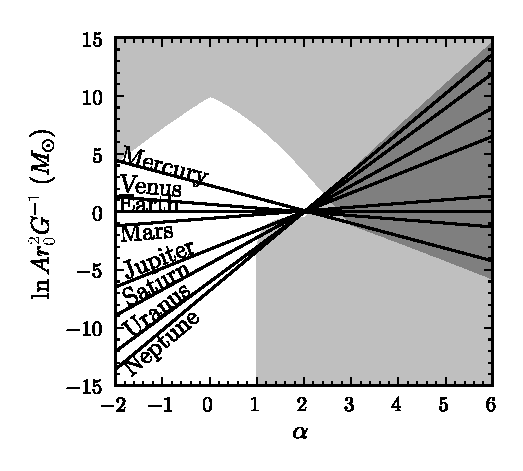
\includegraphics[width=.75\textwidth]{figs_solarsystem/virial_main.ps}
\caption[Virial relation between kinetic and potential energy for each
  of the planets in the Solar System]{The virial relation between the
  kinetic energy and the potential energy
  (equation~[\ref{eq:virialtheorem}]) for each of the eight planets in
  the Solar System. For the combinations of dynamical parameters in
  the light gray region in the lower right at least one planet becomes
  unbound. When the dynamical parameters are in the light gray region
  in the upper left at least one planet has $\rperi<R_\odot$. The
  light gray regions overlap in the dark gray region. In the units
  used in this \figurename, the ``true'' value of $A$ lies at $\ln A
  r_0^2 G^{-1} = 0$.}\label{fig:virial_main}
\end{figure}

\clearpage
\begin{figure}
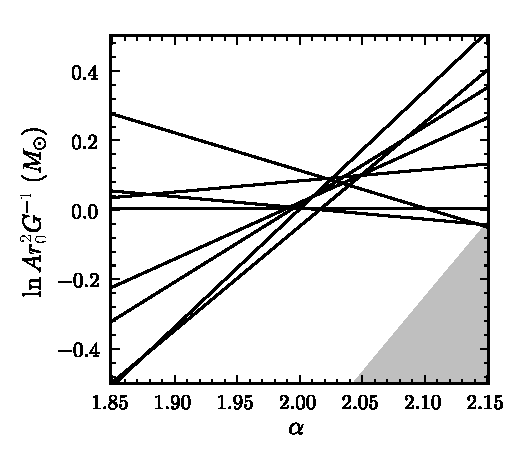
\includegraphics[width=.75\textwidth]{figs_solarsystem/virial_zoom.ps}
\caption{Zoomed in version of \figurename~\ref{fig:virial_main}.}\label{fig:virial_zoom}
\end{figure}

\clearpage
\begin{figure}
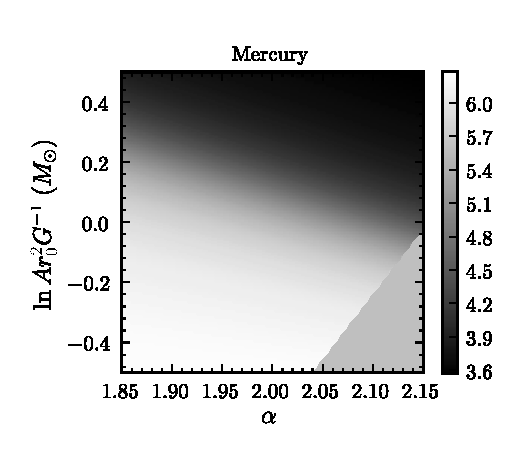
\includegraphics[height=.2\textheight]{figs_solarsystem/phase_Mercury.ps}
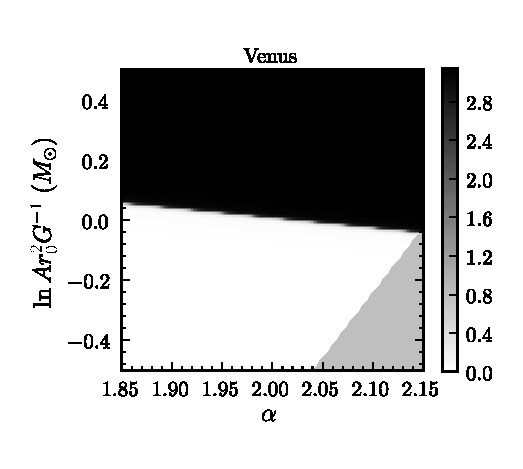
\includegraphics[height=.2\textheight]{figs_solarsystem/phase_Venus.ps}\\
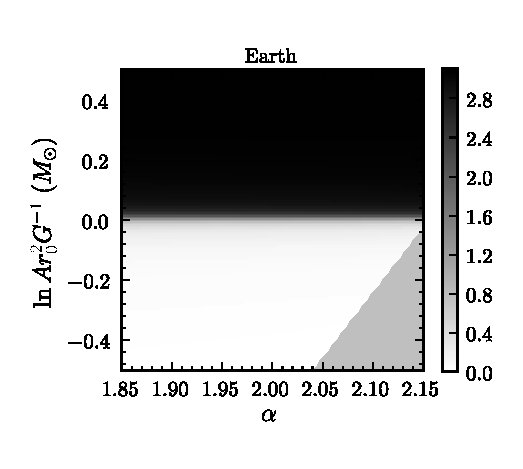
\includegraphics[height=.2\textheight]{figs_solarsystem/phase_Earth.ps}
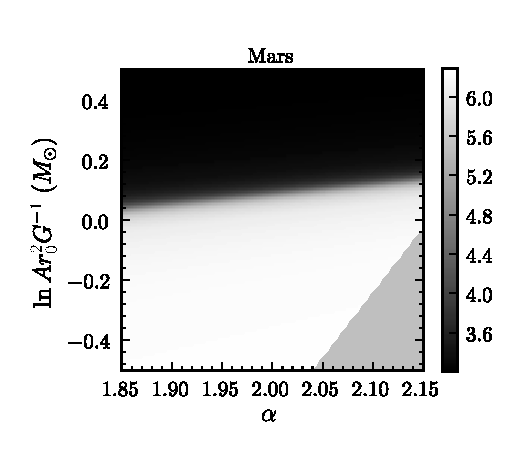
\includegraphics[height=.2\textheight]{figs_solarsystem/phase_Mars.ps}\\
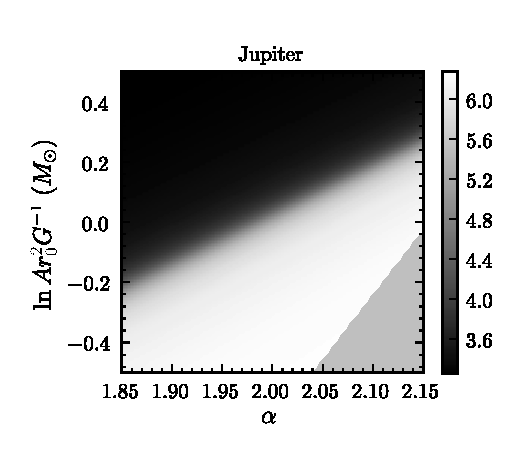
\includegraphics[height=.2\textheight]{figs_solarsystem/phase_Jupiter.ps}
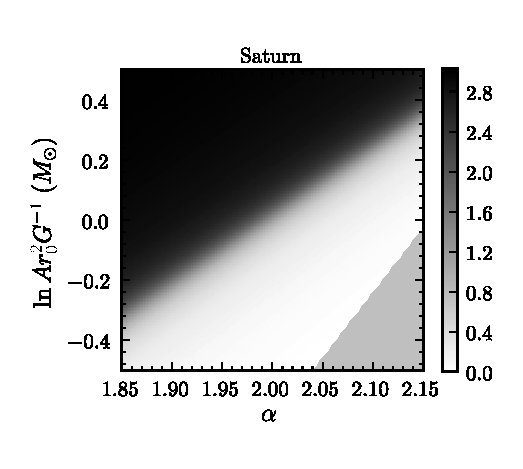
\includegraphics[height=.2\textheight]{figs_solarsystem/phase_Saturn.ps}\\
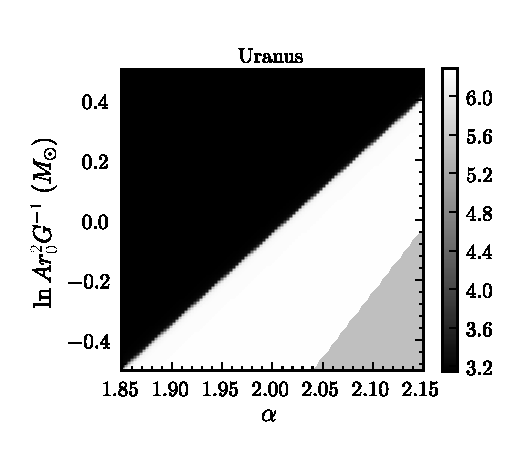
\includegraphics[height=.2\textheight]{figs_solarsystem/phase_Uranus.ps}
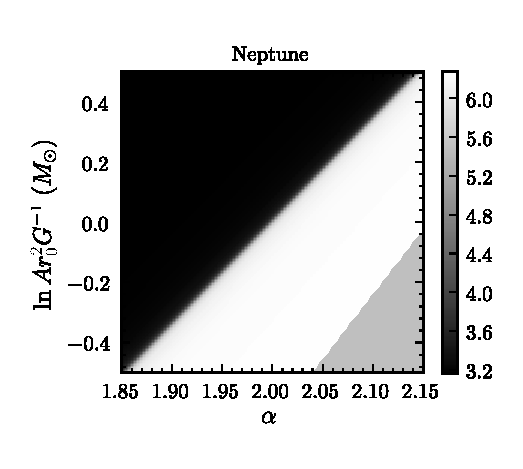
\includegraphics[height=.2\textheight]{figs_solarsystem/phase_Neptune.ps}
\caption[Radial angles for each of the planets as a function of the
  dynamical parameters]{Computed radial angles $\angle$ for each of
  the eight planets as a function of the dynamical parameters. The
  gray triangular region in the bottom-right corner is the region
  excluded by the condition that all the planets are bound.  Each
  planet has an angle range of $0<\angle<\pi$ if it has radial
  velocity $v_r>0$ (outgoing from perihelion) or $\pi<\angle<2\,\pi$
  if it has $v_r<0$ (incoming from
  aphelion).}\label{fig:anglesPlanets}
\end{figure}

\clearpage
\begin{figure}
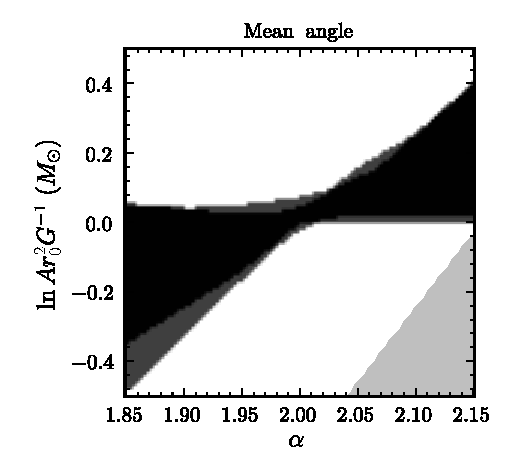
\includegraphics[height=.2\textheight]{figs_solarsystem/freqMean.ps}
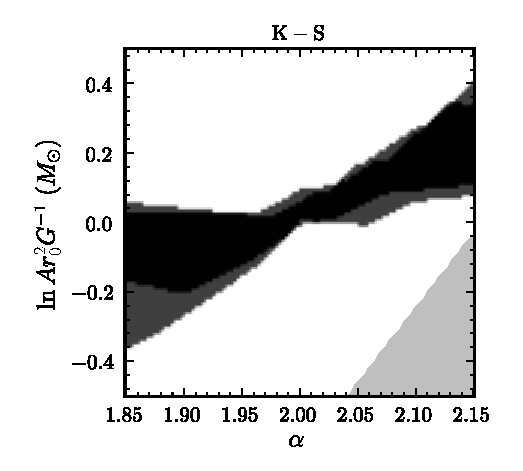
\includegraphics[height=.2\textheight]{figs_solarsystem/freqKS.ps}\\[5pt]
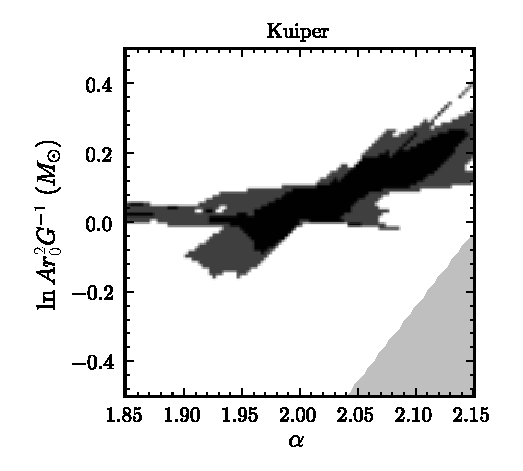
\includegraphics[height=.2\textheight]{figs_solarsystem/freqKuiper.ps}
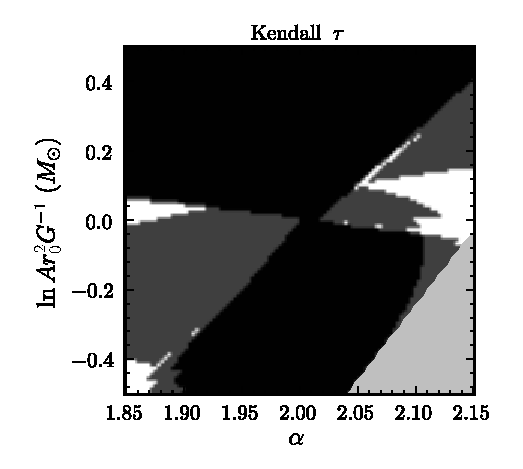
\includegraphics[height=.2\textheight]{figs_solarsystem/freqKendall.ps}\\[5pt]
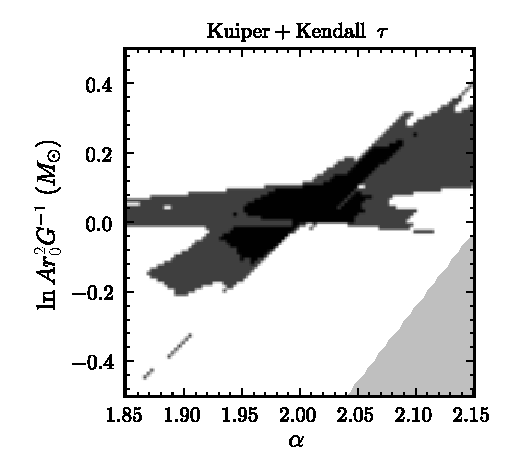
\includegraphics[height=.2\textheight]{figs_solarsystem/freqKuiperKendall.ps}
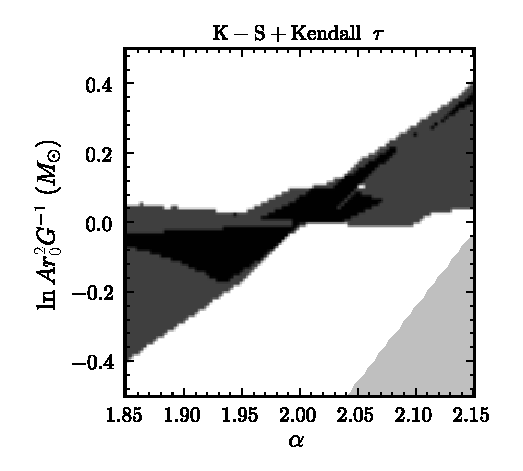
\includegraphics[height=.2\textheight]{figs_solarsystem/freqKSKendall.ps}
\caption[Various frequentist test appied to test the uniformity of the
  angle distribution and the absence of angle-energy
  correlations.]{Various frequentist tests applied to test the
  uniformity of the angle distribution and the absence of angle-energy
  correlations. From top to bottom, left to right: test of the mean of
  the angles; \KS\ test for the uniformity of the angle distribution;
  Kuiper test for the uniformity of the angles; Kendall $\tau$ test
  for the absence of angle-energy correlations; combined confidence
  intervals from the Kuiper test and the Kendall test; combined
  confidence intervals from the \KS\ test and the Kendall test. In the
  plots with a single statistic the darkest region corresponds to the
  95~percent confidence region, the lighter region to the 99~percent
  confidence region. The same is true for the plots with combinations
  of statistics, except that a Bonferroni correction has been applied
  to the significances of the individual statistics that make up the
  combination. In each plot the lightest region is excluded because at
  least one planet becomes unbound for those parameter
  values.}\label{fig:freq}
\end{figure}


\clearpage
\begin{figure}
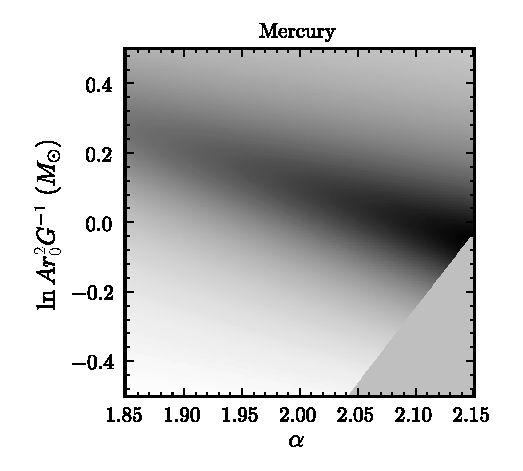
\includegraphics[height=.2\textheight]{figs_solarsystem/jacobian_Mercury.ps}
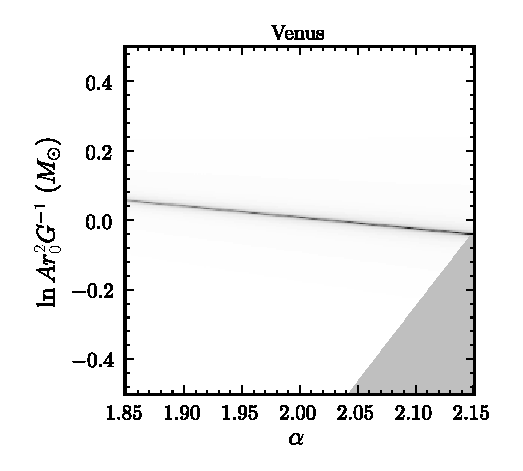
\includegraphics[height=.2\textheight]{figs_solarsystem/jacobian_Venus.ps}\\[5pt]
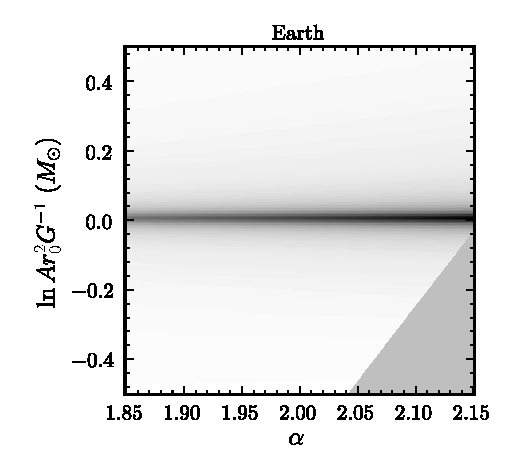
\includegraphics[height=.2\textheight]{figs_solarsystem/jacobian_Earth.ps}
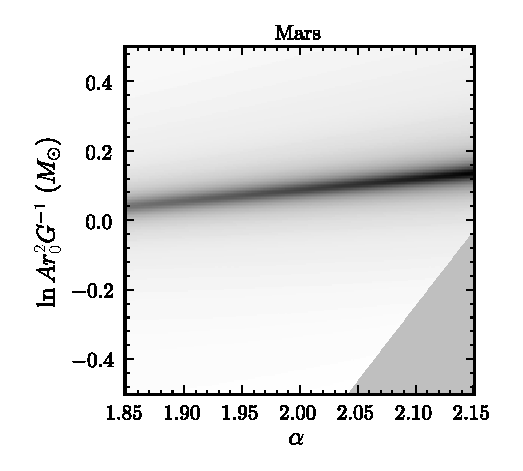
\includegraphics[height=.2\textheight]{figs_solarsystem/jacobian_Mars.ps}\\[5pt]
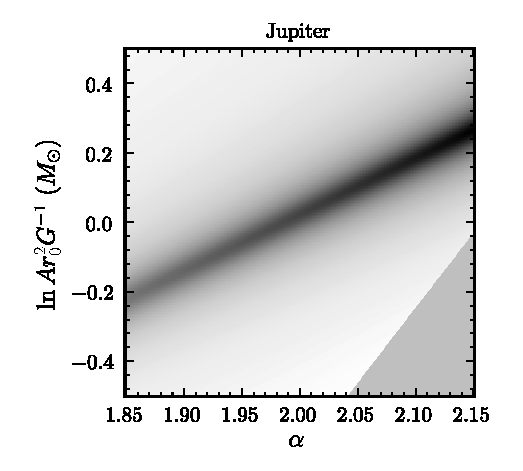
\includegraphics[height=.2\textheight]{figs_solarsystem/jacobian_Jupiter.ps}
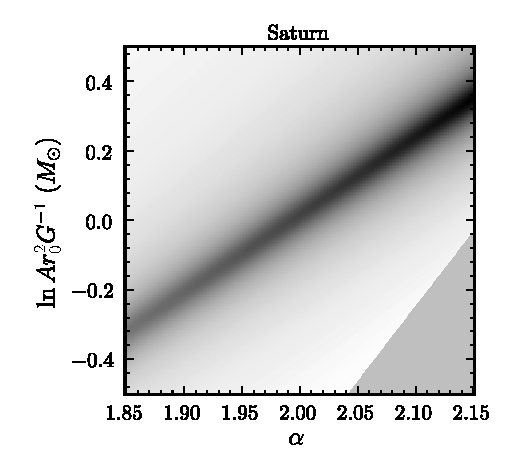
\includegraphics[height=.2\textheight]{figs_solarsystem/jacobian_Saturn.ps}\\[5pt]
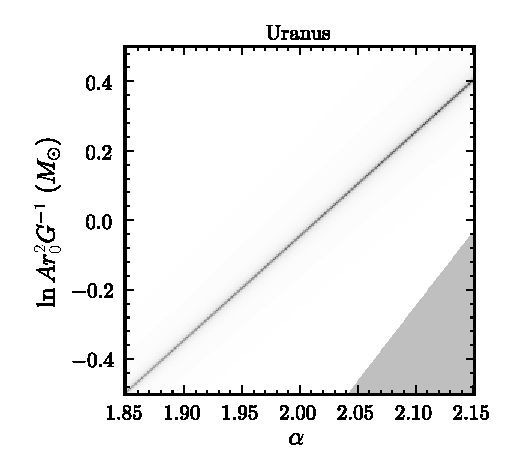
\includegraphics[height=.2\textheight]{figs_solarsystem/jacobian_Uranus.ps}
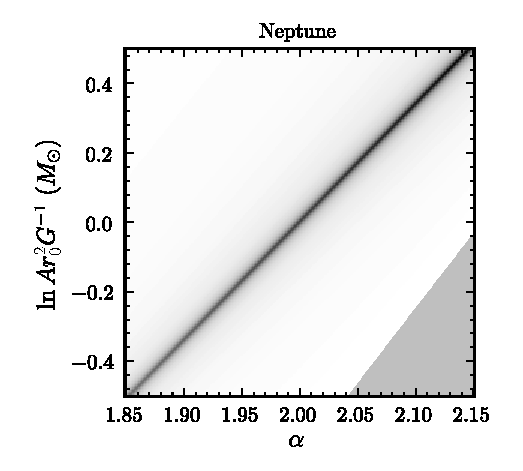
\includegraphics[height=.2\textheight]{figs_solarsystem/jacobian_Neptune.ps}
\caption[Density plots of the absolute value of the determinant of the
  Jacobian of the transformation from the energy, radial asymmetry,
  and radial angle coordinates to the relevant positional and
  kinematical observables]{Density plots of the absolute value of the
  determinant $|J(\lnepsilon,e,\angle;r,v_r,\vperp)|$ of the Jacobian
  of the transformation from the energy $\epsilon$, radial asymmetry
  $e$, and radial angle $\angle$ coordinates to the relevant
  positional and kinematical observables, evaluated at the observed
  positions and velocities of the planets, as a function of the
  dynamical parameters. Grayscales are linear with darker shades for
  larger values.}\label{fig:jacobiansPlanets}
\end{figure}


\clearpage
\begin{figure}
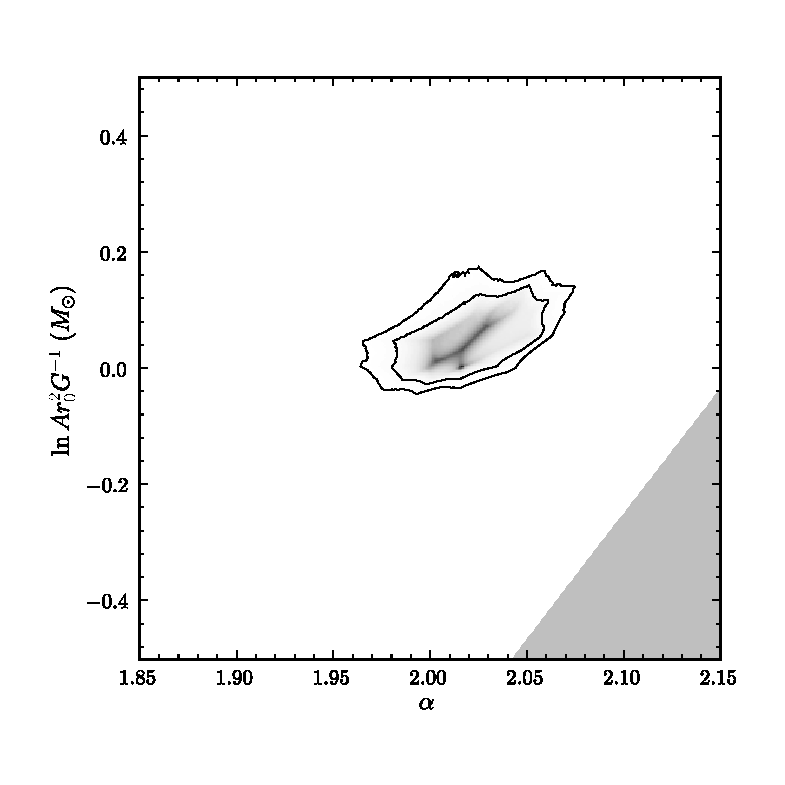
\includegraphics[width=0.6\textwidth]{figs_solarsystem/murrayRoulette.ps}\\%%BoundingBox: 176 285 405 489
\caption[The posterior probability distribution $p(\mvomega|\setofxv)$
  for the dynamical parameters]{The posterior probability distribution
  $p(\mvomega|\setofxv)$ for the dynamical parameters on a linear
  scale. Contours are 95 and 99~percent posterior
  regions.}\label{fig:Bayes2d}
\end{figure}

\clearpage
\begin{figure}
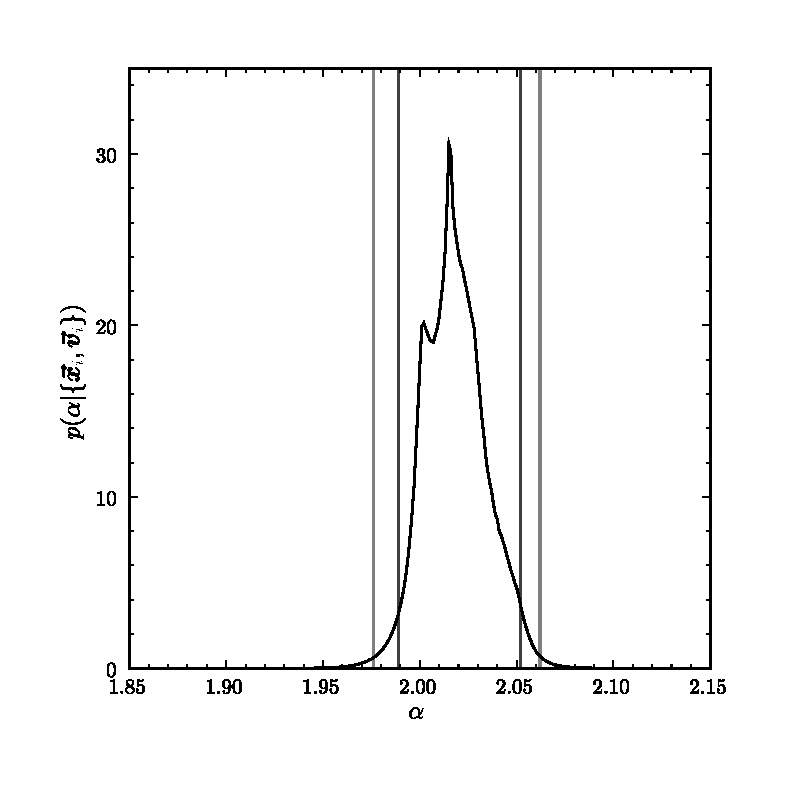
\includegraphics[width=0.6\textwidth]{figs_solarsystem/murrayRouletteAlpha.ps}
\caption{Marginalized posterior probability distribution for the
parameter $\alpha$ with 95 and 99~percent posterior
intervals.}\label{fig:Bayes1d}
\end{figure}

\clearpage
\begin{figure}
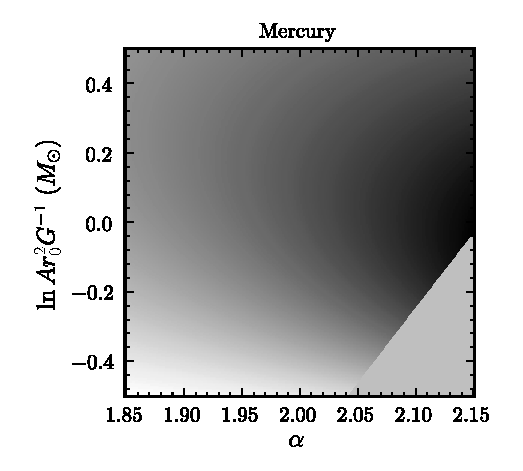
\includegraphics[height=.4\textheight]{figs_solarsystem/ejacobian_Mercury.ps}\\[5pt]
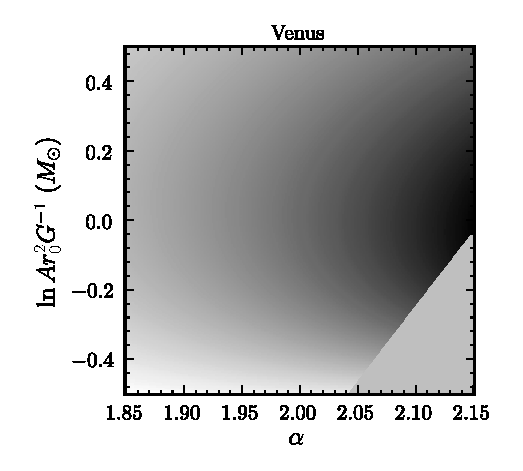
\includegraphics[height=.4\textheight]{figs_solarsystem/ejacobian_Venus.ps}
\caption[Density plots of the absolute value of the determinant of the
  Jacobian of the transformation from the energy, radial asymmetry
  squared, and radial angle coordinates to the relevant positional and
  kinematical observables]{Density plots of the absolute value of the
  determinant $|J(\lnepsilon,e^2,\angle;r,v_r,\vperp)|$ of the
  Jacobian of the transformation from the energy $\epsilon$, radial
  asymmetry squared $e^2$, and radial angle $\angle$ coordinates to
  the relevant positional and kinematical observables, evaluated at
  the observed positions and velocities of the planets, as a function
  of the dynamical parameters. Grayscales are linear with darker
  shades for larger values. Only the Jacobians for Mercury and Venus
  are shown here; the corresponding Jacobians for the other planets
  are very similar to these.}\label{fig:ejacobiansPlanets}
\end{figure}

\clearpage
\begin{figure}
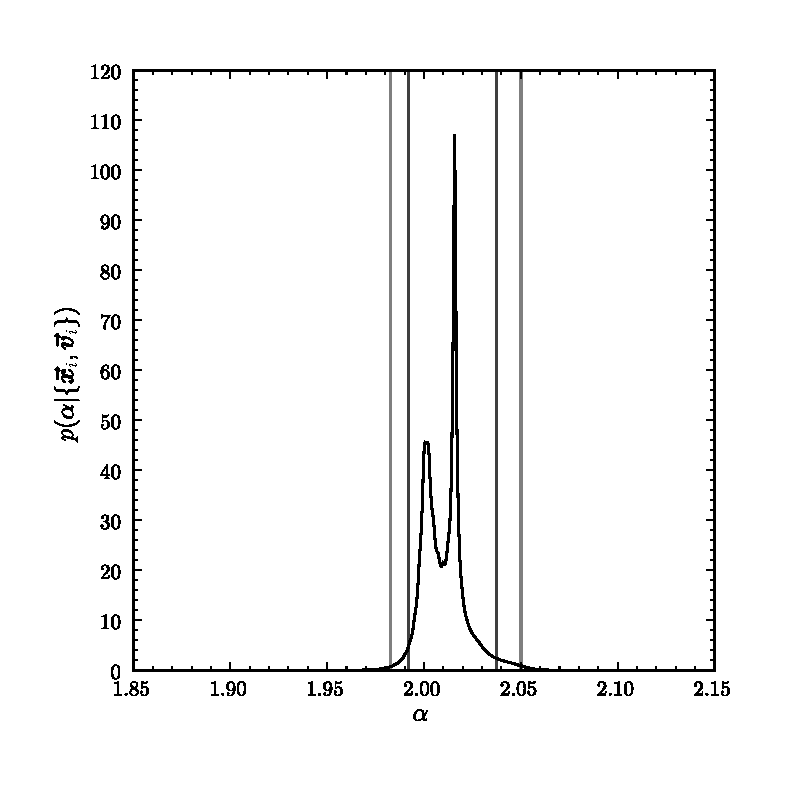
\includegraphics[height=.4\textheight]{figs_solarsystem/alpha_posterior_3es_data6.ps}\\
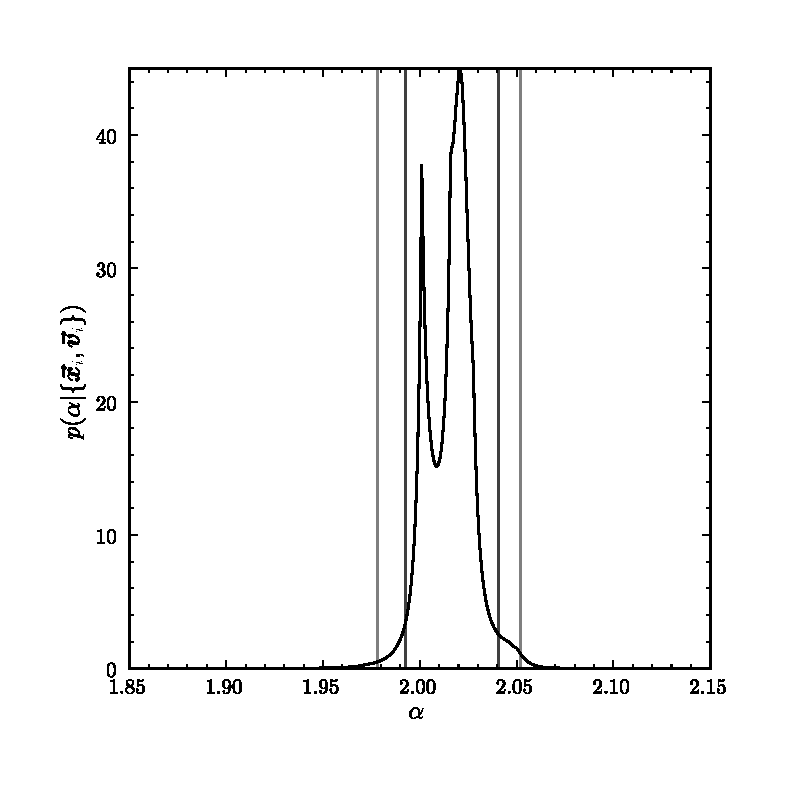
\includegraphics[height=.4\textheight]{figs_solarsystem/alpha_posterior_mcmc_6_500000.ps}
\caption[Alternative posterior probability distributions for the
  parameter $\alpha$]{Alternative posterior probability distributions
  for the parameter $\alpha$ with 95 and 99~percent posterior
  intervals. Top: distribution over radial asymmetry is assumed to be
  uniform in one of $\sqrt{e}$, $e$ or~$e^2$. Bottom: results from a
  non-parametric prior over the distributions of both $e$ and~$\ln
  A$.}\label{fig:altBayes1d}
\end{figure}


\chapter[Galactic masers and the Milky Way circular velocity]{Galactic masers and the Milky Way circular velocity\protect\footnote{Joint work with David~W.~Hogg and Hans-Walter Rix, published as Jo Bovy \etal\ 2009 \emph{ApJ} {\bf 704} 1704. Reproduced by permission of the AAS.}\label{chap:masers}}

\section{Chapter abstract}
Masers found in massive star-forming regions can be located precisely
in six-dimensional phase space and therefore serve as a tool for
studying Milky Way dynamics. The non-random orbital phases at which
the masers are found and the sparseness of current samples require
modeling. Here we model the phase-space distribution function of 18
precisely measured Galactic masers, permitting a mean velocity offset
and a general velocity dispersion tensor relative to their local
standards of rest, and accounting for different pieces of prior
information. With priors only on the Sun's distance from the Galactic
Center and on its motion with respect to the local standard of rest,
the maser data provide a weak constraint on the circular velocity at
the Sun of $\vc = 246 \pm 30$ km s$^{-1}$. Including prior information
on the proper motion of Sgr A$^*$ leads to $\vc = 244 \pm 13$ km
s$^{-1}$.  We do not confirm the value of $\vc \approx 254$ km
s$^{-1}$ found in more restrictive models.  This analysis shows that
there is no conflict between recent determinations of $\vc$ from
Galactic Center analyses, orbital fitting of the GD-1 stellar stream,
and the kinematics of Galactic masers; a combined estimate is $\vc =
236 \pm 11$ km s$^{-1}$. Apart from the dynamical parameters, we find
that masers tend to occur at post-apocenter, circular-velocity-lagging
phases of their orbits.


\section{Introduction}

The value of the circular orbital velocity at the Sun's radius in the
Milky Way is of considerable interest in Galactic and extragalactic
astrophysics. It is necessary to correct observed velocities of stars
and galaxies for the motion of the Sun around the Galactic Center. The
circular velocity also plays a large role in characterizing the mass
of the Milky Way in comparison with other spiral galaxies, placing it
in a cosmological context, \eg, when asking whether the Milky Way
matches the Tully--Fisher relation \citep[\eg][]{Klypin02a,Flynn06a}
or what is its total star formation efficiency
\citep[\eg,][]{Smith07a,Xue08a}.

The circular velocity at the Sun's radius has typically been
established by measuring the Sun's motion with respect to an object
assumed to be at rest with respect to the Galaxy (Sgr A$^*$:
\citealt{Reid04a}; the stellar halo: \citealt{Sirko04a}), or by using
a tracer population assumed to be angle-mixed, \ie, having a uniform
distribution of orbital phases, in a steady-state Galaxy
\citep[\eg,][]{Feast97a}. Recently, a competitive estimate has been
obtained by a different approach using a narrow stellar stream that is
assumed to be tracing out an orbit \citep{Koposov09a}.

In this \chaptername\ we re-analyze a new population of tracers of
Milky Way dynamics: masers associated with star-forming regions
\citep[\reid]{Reid09a}. Using the Very Long Baseline Array (\vlba) and
the Japanese \vlbi\ Exploration of Radio Astronomy (\vera), precise
measurements of the parallaxes, proper motions, and line-of-sight
velocities of masers have been made (see \reid\ and references
therein). These give accurate full six-dimensional phase-space
information in the disk of the Galaxy. Since these massive
star-forming regions are associated with spiral arms and their shocks,
the dense molecular gas regions that produce masers do not lie on
exactly circular orbits, nor are they detected at random points on
their orbits. Therefore, modeling approaches that assume a uniform
distribution of the orbital phases of the tracer population cannot
give accurate determinations of the dynamics of the Galaxy. For the
existing maser data, the problem of non-random orbital phases is
exacerbated by the sparseness of the sample---only 18 masers with
accurate six-dimensional phase-space information have been measured at
present---and by the spatially non-uniform selection of the current
sample of masers.

In this \chaptername, we perform an analysis of the \reid\ maser data
that deals simultaneously with the sparseness of the data, the spatial
non-uniformity of the sampling, the non-random orbital phase
distribution of masers, and prior information. Assuming a flat
rotation curve, $\vc(R) = $ constant, we use a simple model for the
distribution of the maser velocities with respect to their local
standards of rest: a mean offset from circular rotation $\vc(R)$ and a
general velocity dispersion tensor fixed in Galactocentric cylindrical
coordinates. In the probabilistic inference framework that we
use---described in \sectionname~\ref{sec:data}---we can marginalize
over the uncertainty in the inferred distribution function of masers,
take prior information on the dynamics of the Galaxy into account, use
the sparse data set as efficiently as possible, and then ask what
information on $\vc$ the maser data provide. Our results presented in
\sectionname~\ref{sec:results} show that allowing for a finite
velocity dispersion tensor in the model for the maser
peculiar-velocity distribution function leads to lower values of $\vc$
than the large value reported in \reid, in whose analysis the maser
velocity dispersion was (implicitly) assumed to vanish.  Adding in
informative prior information about $R_0$, inferred from monitoring
stellar orbits around the black hole at the center of the Galaxy
\citep{Ghez08a,Gillessen09a} and from the measurement of the proper
motion of Sgr A$^*$ \citep{Reid04a}, we find that the best circular
velocity estimate is $\vc = 244 \pm 13$ km s$^{-1}$, but that the
current maser data set adds little information. We discuss this
measurement and its limitations in the light of other recent
determinations in \sectionname~\ref{sec:discussionmasers}.


\section{Data and methodology}\label{sec:data}

Throughout the analysis that follows we use the standard cylindrical
Galactocentric coordinate frame $(R,\phi,z)$, with associated unit
vectors ($\eeR,\eephi,\eezmasers$) pointing toward the Galactic
center, in the direction of Galactic rotation, and toward the North
Galactic Pole, respectively.

\subsection{Data from \protect\citet{Reid09a}}\label{sec:datasub}

The data we analyze here consist of the Galactic coordinates,
parallaxes, proper motions, and line-of-sight velocities of 18
Galactic masers, as well as their associated uncertainties, presented
in Table 1 of \citet{Reid09a}. Following \reid, we add a 7 km s$^{-1}$
uncertainty in quadrature to the uncertainties in the velocity
components of each maser to describe the random, virial motion in the
massive star-forming region of the individual massive star associated
with each maser.

The line-of-sight velocities have been `corrected' by the radio
observatories' pipelines for the motion of the Sun with respect to the
Local Standard of Rest (\lsr). This correction assumed a value of 20
km s$^{-1}$ toward \ra(B1900.0)= 18$^\mathrm{h}$,
\dec(B1900.0)=$+30\degree$ for the Solar motion \vsunlsr, although it
is unclear whether all observatories used this standard value
(M.~Reid, private communication). We undo this correction, after
which the currently accepted correction for \vsunlsr\ can be applied;
however, as we will describe below, this correction will become part
of our model and, therefore, the correction for \vsunlsr\ does not
occur during the preprocessing of the data.

Beyond these two corrections, no processing of the \citet{Reid09a}
data has been done.


\subsection{Probabilistic framework}

Parameter estimation in a probabilistic framework \emph{by necessity}
uses Bayes's theorem to connect the probability of the model
parameters given the data
$\{\vxi^{\mathrm{obs}},\vvi^{\mathrm{obs}}\}$ to the probability of
the observed data given the model parameters
\citep[\eg,][]{jaynes}. This requires us (1) to identify all the
parameters that need to be included in the model, (2) to write down
the likelihood of the model and (3) to specify suitable priors for the
model parameters. Although the model space needs to be exhaustive, the
probabilistic framework allows integration over uninteresting
parameters.

Here we put forward a model for the maser kinematics in which the
maser velocities are most easily modeled in Galactocentric cylindrical
coordinates. In order to go from the raw data described in
\sectionname~\ref{sec:datasub} to the velocity of each maser in
Galactocentric coordinates, we need to (1) correct the measured
velocity for \vsunlsr, (2) add to this velocity the circular velocity
around the Galactic center at the Sun's radius, and (3) project this
velocity onto the Galactocentric coordinate frame (the details of this
transformation are described in the Appendix of \reid). Since the
latter procedure includes geometrical projection factors depending on
the distance \Ro\ of the Sun from the Galactic Center, the model
parameters need to include the three components of \vsunlsr, \Ro, and
$\vc$. However, it is more practical to assume that Sgr A$^*$ is at
rest with respect to the Galaxy, and to use the proper motion
$\pmsgra$ of Sgr A$^*$ \citep{Reid04a} as a model parameter instead of
the circular velocity, as $\pmsgra$ is very tightly constrained
independently of $R_0$. These two parameters are related simply by
multiplying the proper motion of Sgr A$^*$ by $R_0$ and correcting
this for \vsunlsr. The circular velocity then becomes a parameter
derived from the actual model parameters, which is no problem in the
probabilistic framework, where it is easy to propagate uncertainties
correctly.  As we will assume that the rotation curve is flat, no
extra parameters to model the shape of the rotation curve need to be
included in the model.

If we had uniformly sampled the phase space of masers and full prior
knowledge of the phase-space distribution function of massive
star-forming regions, this would uniquely specify the likelihood of
the model, as the probability of the measured position and velocity of
each maser would simply be given by the distribution function of the
masers convolved with the observational uncertainty. However, we have
neither a uniform sample of masers nor much prior information about
the distribution of masers throughout the Galaxy. To account for the
spatial non-uniformity of the sample we will focus on the distribution
of velocities at the actually observed position of the maser, instead
of using the full six-dimensional phase-space distribution function to
evaluate the likelihood. For this distribution we will assume that it
only depends on the peculiar velocity $\vvpec \equiv \vvmaser - \vc
\cdot \eephi$ of the maser in Galactocentric cylindrical
coordinates. We will assume that this distribution of peculiar
velocities is given by a Gaussian distribution characterized by a
mean, a 3-vector $\masermean$, the offset from circular motion, and a
general velocity dispersion tensor, a symmetric $3 \times 3$ tensor
$\maserdisp$ with six free parameters. Since there have been no
measurements of either the mean offset from circular motion of the
masers or their velocity dispersion, we will use flat priors on these
quantities. This model is essentially a generalization of the model
used in \citet{Reid09a} where the velocity dispersion tensor was
assumed to vanish; this was a poor assumption as we will show below.

The probability of a single maser is thus given by
\begin{equation}\label{eq:onelike}
p(\vxi^{\mathrm{obs}},\vvi^{\mathrm{obs}}|\pmsgra,R_0,\vsunlsr,\masermean,\maserdisp) =
\normal\left(\vvpec[\vx,\vv]|\masermean,\maserdisp\right)\otimes p(\vx,\vv|\vxi^{\mathrm{obs}},\vvi^{\mathrm{obs}})\,,
\end{equation}
where we have suppressed the dependence of $\vvpec$ on the dynamical
parameters, and where the convolution with the observational
uncertainty distribution
$p(\vx,\vv|\vxi^{\mathrm{obs}},\vvi^{\mathrm{obs}})$ has been
included. The posterior distribution for the 14 model parameters is
then given by
\begin{equation}\label{eq:posterior}
\begin{split}
p(\pmsgra,R_0,\vsunlsr,\masermean,\maserdisp|\{\vxi^{\mathrm{obs}},\vvi^{\mathrm{obs}}\})
\propto & \ p(\pmsgra,R_0,\vsunlsr)\\
& \times \prod_i
p(\vxi^{\mathrm{obs}},\vvi^{\mathrm{obs}}|\pmsgra,R_0,\vsunlsr,\masermean,\maserdisp)\,,
\end{split}
\end{equation}
where the first factor on the right-hand side is the prior probability
distribution for these parameters and the product is the
likelihood. We have used flat priors for $\masermean$ and
$\maserdisp$, which is why they do not appear explicitly.

For $\pmsgra$ we use a Gaussian prior with a mean of 30.24 km s$^{-1}$
kpc $^{-1}$ and a standard deviation of 0.12 km s$^{-1}$ kpc$^{-1}$
\citep{Reid04a}. For \Ro\ we combine current state-of-the-art
determinations of \Ro\ from Galactic Center orbits with equal weights:
8.0 $\pm$ 0.6 kpc found by \citet{Ghez08a} and 8.33 $\pm$ 0.35 kpc
found by \citet{Gillessen09a}. This prior is shown as the gray curve
in \figurename~\ref{fig:ro}. For \vsunlsr\ we use the value and
uncertainties obtained from \emph{Hipparcos} data
\citep{2005ApJ...629..268H}, although the clumpiness of the velocity
distribution of nearby stars \citep{1998AJ....115.2384D,Bovyveldist}
implies an uncertainty more on the order of a few km s$^{-1}$ in the
value of \vsunlsr\ (J.~Bovy \& D.~W.~Hogg, in preparation). The
implied prior for the circular velocity is shown as the thick gray
curve in \figurename~\ref{fig:thetao}. To investigate how informative
the maser measurements are about $\vc$ and $R_0$, we will consider the
effect of dropping (some combination of) these priors below.

The framework described here can easily be generalized to more general
descriptions of the distribution of the peculiar velocities of the
masers. In what follows we will use a distribution function that is
the sum of two Gaussian distributions, the second having half of the
weight and twice the dispersion of the first Gaussian, to determine
the possible effect of outliers.

\subsection{Exploration of the posterior probability distribution}

In order to explore the posterior distribution for all of the model
parameters in light of the maser data we use a simple Markov Chain
Monte Carlo (MCMC) method \citep{mackay}. This procedure is described
in some detail in the Appendix.

The practical complication in evaluating the likelihood given in
\eqnname s~(\ref{eq:onelike}) and (\ref{eq:posterior}) for each of the
masers comes from the fact that the observational uncertainties are
Gaussian in the space of observed quantities---more specifically, for
the parallax---but are non-Gaussian in the space of the peculiar
velocities. However, if the relative parallax uncertainty is small
($\leq 10$\,percent) we can confidently propagate the uncertainties to
the space of peculiar velocities, where the convolution of the
Gaussian velocity distribution model for the peculiar velocities with
the observational Gaussian uncertainty distribution is simple. A few
of the masers have relative parallax uncertainties larger than
10\,percent, but we have nonetheless propagated the uncertainties in
the Gaussian approximation. To check that this does not bias our
results we have also run our analysis using a full numerical
convolution with the actual observational uncertainties and we find
results that are barely distinguishable from the results presented
below.


\section{Results}\label{sec:results}

The main scientific goal of this \chaptername\ is to understand what
the maser measurements tell us about $\vc$. The posterior probability
distribution for $\vc$, fully marginalized over all of the parameters
of the maser distribution function, the Solar motion with respect to
the \lsr, the distance to the Galactic Center, and the proper motion
of Sgr A$^*$, is shown in \figurename~\ref{fig:thetao}. The
analogously marginalized posterior distribution for \Ro\ is shown in
\figurename~\ref{fig:ro}. Also shown in \figurename~\ref{fig:thetao}
is the posterior we obtained when we drop the informative prior on
$\pmsgra$. The posterior distributions for the proper motion of Sgr
A$^*$ and for the components of \vsunlsr\ are not shown here. They are
all basically identical to their prior distributions, implying that
the masers---not surprisingly---cannot inform us about these
quantities.

While the prior on $\vc$ in \figurename~\ref{fig:thetao} peaks at 244
km s$^{-1}$ with a 1--sigma uncertainty of 16 km s$^{-1}$, the
posterior for $\vc$ is peaked at a value of 244 km s$^{-1}$ with a
1--sigma uncertainty of about 13 km s$^{-1}$. This equal value for
$\vc$ after analyzing the masers is in qualitative contrast to the
initial analysis of \reid, who found that it raised the peak to 254 km
s$^{-1}$. This difference arises mainly from our more general model
for the distribution function of the masers. If we insist within our
analysis that the velocity dispersion of the masers is zero, we find a
posterior distribution for the circular velocity that is peaked at 255
km s$^{-1}$, in rough agreement with the \reid\ results. The light
gray line in \figurename~\ref{fig:thetao} shows what happens when we
drop the informative prior on $\pmsgra$, while keeping the $R_0$
prior: $\vc = 246 \pm 30$ km s$^{-1}$. This and the fact that the
posterior probability is barely narrower than the prior, tells us that
the current maser measurements have not much power to constrain
$\vc$. The posterior estimate for the distance to the Galactic Center
is $R_0 = 8.2 \pm 0.4$ kpc; this shows that the masers lead to a small
improvement to our knowledge of the Sun's distance to the Galactic
Center. Without the informative prior on $\pmsgra$ the posterior
estimate for $R_0$ is the same as the prior estimate: $R_0 = 8.2 \pm
0.5$ kpc.

At the same time, the MCMC procedure provides fully marginalized
posterior distributions for the parameters of the conditional velocity
distribution function of masers, which are given in
\figurename~\ref{fig:dist}: shown are the posterior distributions for
the three components of the mean offset from circular velocity of the
masers, \ie, the mean peculiar velocity, in cylindrical coordinates
(toward the Galactic Center, in the direction of Galactic rotation,
and toward the North Galactic Pole) as well as for the trace of the
velocity dispersion tensor. From this we confirm the mean lag of 15 km
s$^{-1}$---we find a lag of $14 \pm 5$ km s$^{-1}$---of the masers
with respect to their local standards of rest previously found by
\reid. \figurename~\ref{fig:dist} shows that the masers have a mean
velocity toward the Galactic Center of $7 \pm 6$ km s$^{-1}$. Taken
together, these mean peculiar velocities imply that the masers are
typically just past the apocenter of their orbits. We also find a mean
velocity component of $3 \pm 3$ km s$^{-1}$ in the direction toward
the North Galactic Pole.

From the posterior distribution for the trace of the velocity
dispersion tensor we see that the masers have a relative large
velocity dispersion---$\trace(\maserdisp)\sim\![29$ km
  s$^{-1}$]$^2$---larger than might be expected from a comparison with
the velocity dispersion of young stars in the Solar neighborhood,
whose trace is about [14 km s$^{-1}$]$^2$
\citep{2005ApJ...629..268H}. Since we put no restrictions on the form
of $\maserdisp$ we also obtain posterior probability distributions for
all of the components of $\maserdisp$: for the diagonal components we
find $\sqrt{\maserdisp_{RR}} = 22 \pm 8$ km s$^{-1}$,
$\sqrt{\maserdisp_{\phi\phi}} = 18 \pm 7$ km s$^{-1}$, and
$\sqrt{\maserdisp_{zz}} = 12 \pm 5$ km s$^{-1}$. As we discuss below,
the fact that we obtain these large values could be because our model
for the conditional velocity distribution is too restrictive.
%Components:
%7.41021362368 5.89694170976
%-13.7869695856 5.36312850468
%-3.26296506761 3.46929349829
%<trV> = 1100, sigma = 760

In order to assess the possible affect of outliers on our inference,
we have performed the same analysis assuming a distribution of the
peculiar velocities which consists of a mixture of two Gaussian
distributions, identical in every aspect except that the second
Gaussian has half of the weight and twice the dispersion of the first
Gaussian (by doubling each component of the velocity dispersion
tensor). We find the same posterior distributions for the dynamical
parameters and the mean offset; the inferred dispersion of the masers
is, predictably, somewhat smaller: the trace of the covariance matrix
peaks at [22 km s$^{-1}$]$^2$. Two specific candidate outliers, the
sources NGC 7538 and G 23.6-0.1, were identified and removed from the
sample by \reid, because they displayed large post-fit residuals. To
assess whether these two sources affect our results significantly, the
same analysis as described above of the \reid\ basic sample of 16
masers was performed, leaving out the sources NGC 7538 and
G~23.6-0.1. We find basically the same result: $\vc = 245 \pm 13$ km
s$^{-1}$. Thus, as opposed to \reid, who found that these two sources
significantly raise the circular velocity derived from the maser data,
our result is robust with respect to their inclusion.

\section{Discussion}\label{sec:discussionmasers}

We have re-analyzed the recent maser kinematics from \reid, to see
what they tell us about $\vc(R_0)$ and the maser orbits. Our analysis
differs from that of \reid\ by allowing for a more general model for
the distribution of the velocities of the masers with respect to their
local standards of rest, by using a proper probabilistic framework
that includes proper marginalization over uninteresting parameters,
and by the explicit inclusion of suitable prior information. From
this, we find an estimate of $\vc$ of $244 \pm 13$ km s$^{-1}$, the
same value as the mode of our prior, and substantially lower than the
estimate of \reid. Our analysis has also shown that the current maser
measurements have only limited power to constrain $\vc$ beyond the
prior; dropping the prior coming from the measured proper motion of
Sgr A$^*$ we find $\vc = 246 \pm 30$ km s$^{-1}$; further dropping the
prior information on $R_0$, the maser data provide no constraint on
$\vc$ at all.

The value for $\vc$ that we have inferred in this \chaptername\ from
the kinematics of Galactic masers compares favorably with other recent
measurements of the circular velocity. As is clear from
\figurename~\ref{fig:thetao}, the posterior probability distribution
for the circular velocity is peaked at about the same value as the
prior probability distribution obtained from combining the precise
measurements of the distance to the Galactic Center, the proper motion
of Sgr A$^*$, and the Solar motion in the direction of Galactic
rotation. It is also consistent with the value of $\vc = 221 \pm 18$
km s$^{-1}$ from a recent measurement based on the completely
different principle of fitting an orbit to the GD-1 stellar stream
\citep{Koposov09a}. Combining these estimates by inverse variance
weighting we find a value for the circular velocity of $\vc = 236 \pm
11$ km s$^{-1}$.

The results in this \chaptername\ are unaffected by the uncertainty in
the value of the Solar motion with respect to the \lsr. If we use a
larger uncertainty in the value of $\vsunlsr$ of 3 km s$^{-1}$ in each
component, as suggested by an analysis of the effect of moving groups
on $\vsunlsr$ (J.~Bovy \& D.~W.~Hogg, in preparation), we retrieve the
same estimate $\vc = 244 \pm 14$ km $^{-1}$ as before. Even when we
use an uncertainty of 15 km s$^{-1}$ in the value of each component of
$\vsunlsr$, we find a slight increase in the uncertainty, but still
the same value $\vc = 244 \pm 20$ km s$^{-1}$. Thus, the uncertainty
in $\vsunlsr$ only affects our conclusions if it is larger than about
10 km s$^{-1}$.

We also learned that the masers on average lag $\vc$ and are moving
toward the Galactic Center. This fact is illustrated in \figurename
s~\ref{fig:dist} and \ref{fig:phases}, where the orbital phases of the
masers are shown for a logarithmic potential $\Phi = \vc^2 \,\ln r$
\citep[\eg, \eqnname~(3.14) in][]{2008gady.book.....B} assuming $R_0 =
8.2$ kpc and $\vc = 244$ km s$^{-1}$. This will be interesting to
analyze in the context of spiral shock models.

Our analysis implies that the present maser data do not lead to a
substantive improvement of our knowledge of \Ro\ and $\vc$, as most of
the information in the data is spent on determining the properties of
the conditional velocity distribution of the masers. It is also
remarkable that, given all of the prior information, the masers are
much more informative about \Ro\ than they are about the angular
rotation speed at the Sun's radius, as the posterior distribution for
$\Omega_0$ is barely distinguishable from the prior distribution.

Despite the fact that most of the information content in the maser
data is already being used to infer the distribution function, it is
possible that our model for the distribution function is not general
enough. For one, it is very likely that the distribution function of
the masers depends on the Galactocentric radius and, in particular,
that the mean velocity offset in the direction toward the Galactic
center depends on radius. Indeed, there is some indication of that
already in our results, as the large velocity dispersion of the masers
is mostly driven by a large velocity dispersion in the direction
toward the Galactic Center; this could be due to an unmodeled radial
dependence of the distribution function.

The measurement of the dynamics of the Galaxy performed here uses a
tracer population that is obviously non-angle mixed but has no
unambiguous non-angle-mixed interpretation---such as a stellar stream
tracing out an orbit. Such a measurement has the fundamental problem
that structure in the distribution function of the tracers is, in a
sense, exchangeable with complexity of the potential. Therefore,
detailed measurements of the potential of the Galaxy using larger
samples of masers will very likely be fundamentally limited by our
lack of knowledge about the distribution function of the masers. As
more masers with precise kinematic information become available---as
many as 400 are possible over the next few years (M.~Reid, private
communication)---more detailed inferences of the distribution function
will have to be made simultaneously with more precise measurements of
the potential of the Galaxy from these masers. The method described
and used in this \chaptername\ is flexible enough to handle these more
general distribution functions and more general models for the
potential of the Galaxy.

BOVY: WHAT TO DO ABOUT THIS APPENDIX?
%\appendix

\section{MCMC exploration of the posterior distribution}\label{sec:mcmc}

We explore the posterior probability distribution using a
Metropolis-Hastings (MH) MCMC algorithm \citep[\eg,][]{mackay}. The MH
algorithm works by proposing new model parameters $x'$ from a proposal
distribution $Q(x';x^{(t)})$ that can only depend on the current
values $x^{(t)}$ of the parameters. One then computes the quantity
\begin{equation}
a =
\frac{p(x'|\setofxv)\,Q(x^{(t)};x')}{p(x^{(t)}|\setofxv)\,Q(x';x^{(t)})}\,.
\end{equation}
If $a \geq 1$ one accepts the new state; if $a < 1$, the new state is
accepted with probability $a$. If the new state is rejected, the old
state is added again as a sample of the posterior. This procedure
converges to give samples from the posterior.

As proposal distributions we use: (1) the prior for the components of
\vsunlsr, (2) a Gaussian for \Ro\ and $\pmsgra$ centered on the
current values with widths of 0.5 kpc and 0.12 km s$^{-1}$ kpc$^{-1}$,
respectively, (3) a Gaussian for the mean offset centered on the
current values with a width of $\sim\!10$ km s$^{-1}$ for each
component, and (4) a Wishart distribution for the velocity dispersion
tensor with mean equal to the current tensor and shape parameter
$\sim\!20$. The widths of these last three proposal distributions were
chosen so as to give an acceptable acceptance rate of about
50\,percent. Monte Carlo chains were run with different sets of
parameters of the proposal distributions and the resulting posterior
probability distributions were found to be independent of the
parameters of the proposal distributions.


\clearpage
\begin{figure}
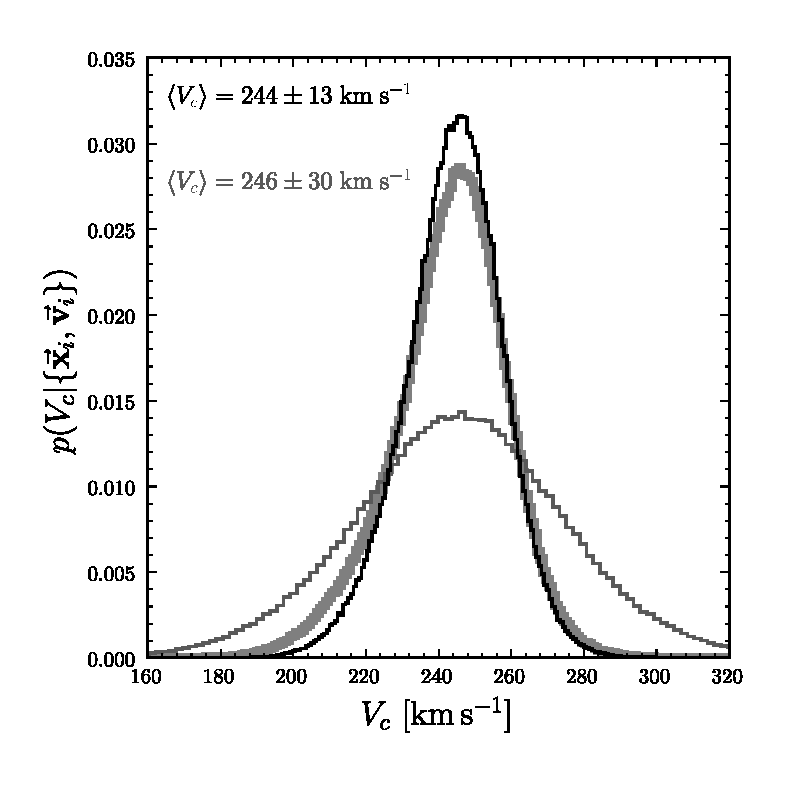
\includegraphics[width=.46\textwidth]{figs_masers/thetao_1M.eps}
\caption[Marginalized posterior probability distribution for the
  circular velocity]{Marginalized posterior probability distribution
  for the circular velocity $\vc$, shown as the black curve, and its
  mean (top label) from 10$^6$ MCMC samples. The prior probability
  distribution is shown as the thick gray curve; its mean is $\vc =
  243 \pm 16 $ km s$^{-1}$. The posterior and its mean (bottom label)
  obtained from dropping the informative prior on $\pmsgra$ is shown
  as the thin gray curve, illustrating that the maser data themselves
  constrain $\vc$ relatively weakly. The quoted uncertainty in mean
  value is the standard deviation $\equiv \sqrt{\langle \vc^2\rangle -
    \langle \vc\rangle^2}$.}\label{fig:thetao}
\end{figure}

\clearpage
\begin{figure}
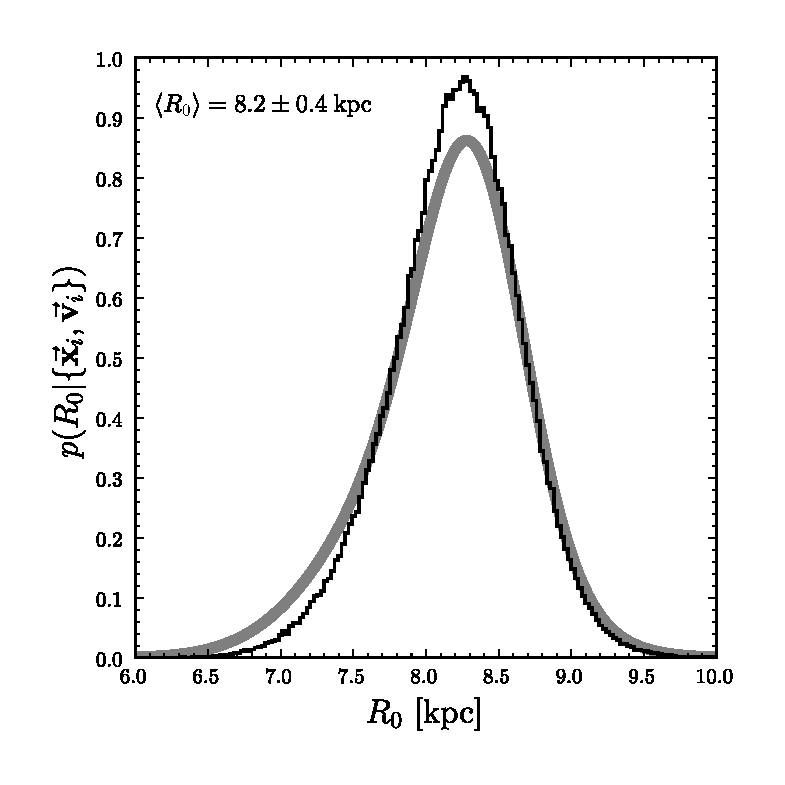
\includegraphics[width=.46\textwidth]{figs_masers/ro_1M.eps}
\caption[Marginalized posterior probability distribution for the
  distance to the Galactic center]{Marginalized posterior probability
  distribution for the distance \Ro\ to the Galactic center, shown as
  the black curve, from 10$^6$ MCMC samples. The prior probability
  distribution is shown as the thick gray curve; its mean is $R_0 =
  8.2 \pm 0.5$ kpc.}\label{fig:ro}
\end{figure}


\clearpage
\begin{figure}
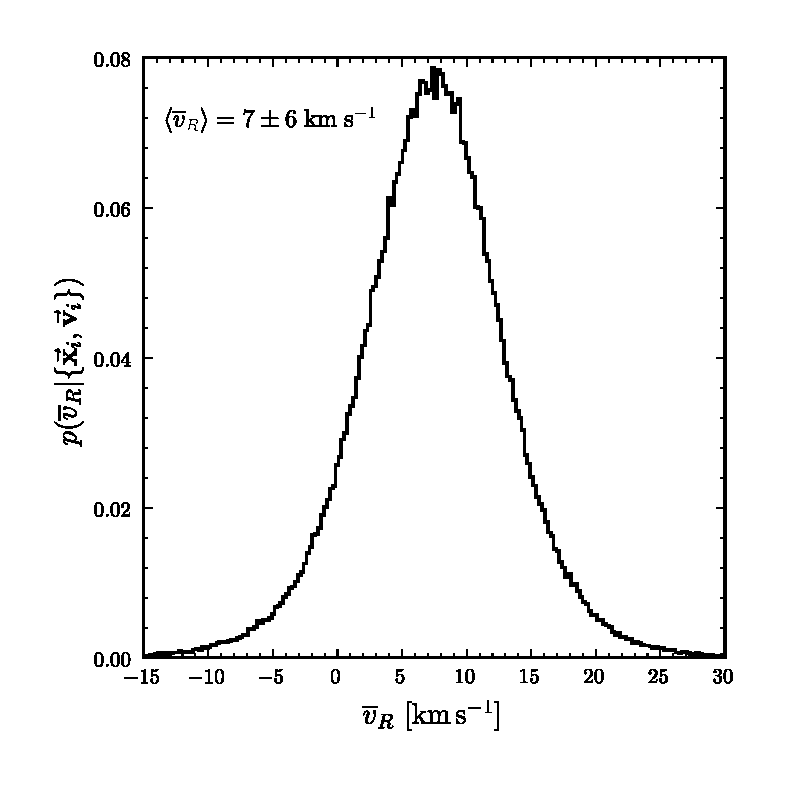
\includegraphics[width=.46\textwidth]{figs_masers/mean_1M_R.eps}
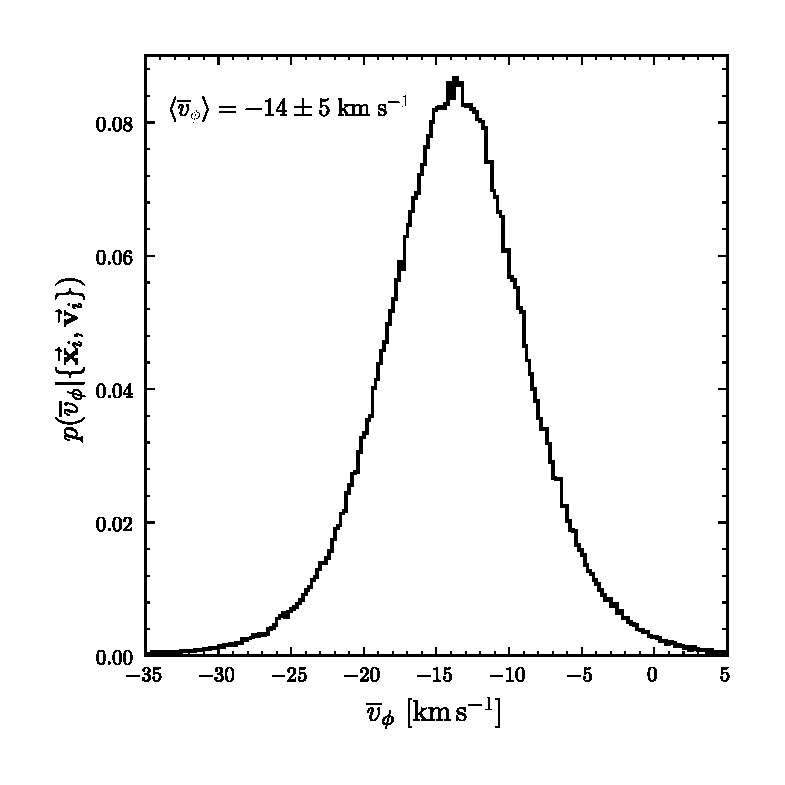
\includegraphics[width=.46\textwidth]{figs_masers/mean_1M_phi.eps}\\
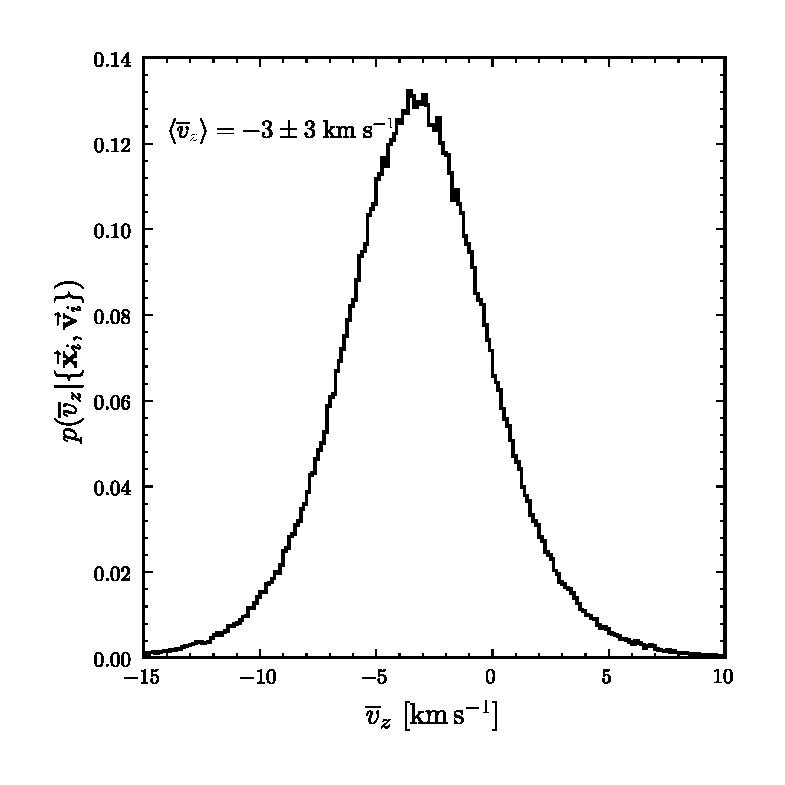
\includegraphics[width=.46\textwidth]{figs_masers/mean_1M_z.eps}
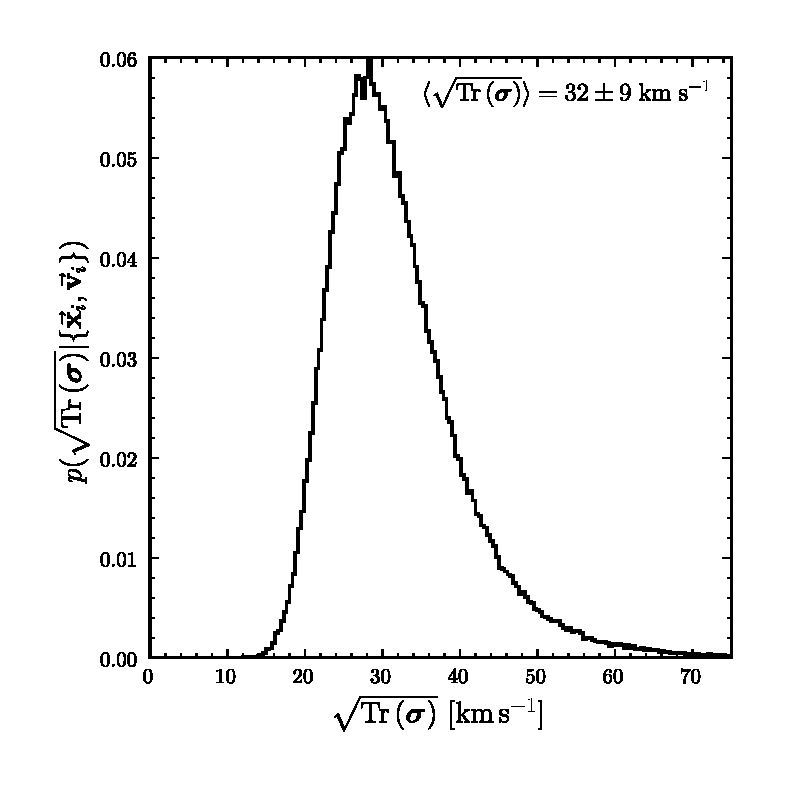
\includegraphics[width=.46\textwidth]{figs_masers/trV_1M.eps}
\caption[Marginalized posterior probability distribution for the
  parameters of the conditional velocity distribution of
  masers]{Marginalized posterior probability distribution for the
  parameters of the conditional velocity distribution of masers from
  10$^6$ samples: mean motion toward the Galactic Center (\emph{top
    left panel}); in the direction of Galactic rotation (\emph{top
    right panel}); toward the North Galactic Pole (\emph{bottom left
    panel}); the square root of the trace of the velocity dispersion
  tensor (\emph{bottom right panel}).}\label{fig:dist}
\end{figure}

\clearpage
\begin{figure}
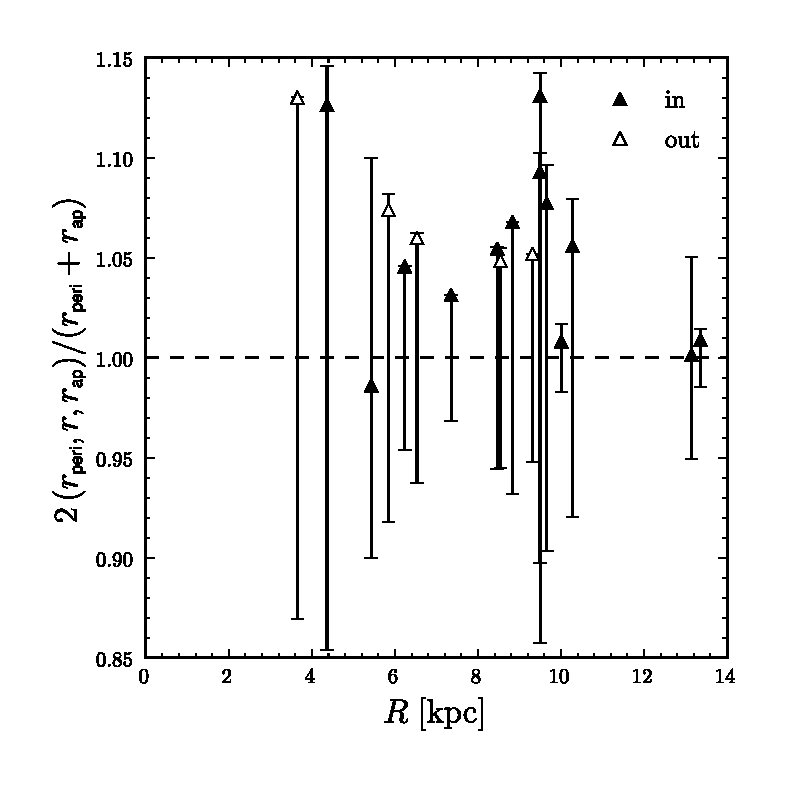
\includegraphics[width=.45\textwidth]{figs_masers/rrperirap.eps}
\caption[Orbital eccentricities and phases of the observed
  masers]{Orbital eccentricities and phases of the observed masers in
  a logarithmic potential: pericenter radius $r_{\mathrm{peri}}$,
  apocenter radius $r_{\mathrm{ap}}$, and current radius of the
  masers, normalized by the mean of the pericenter and apocenter
  radii, as a function of Galactocentric radius in a spherically
  symmetric logarithmic potential for $R_0 = 8.2$ kpc and $\vc = 244$
  km s$^{-1}$. Filled symbols indicate that the maser is moving toward
  the Galactic Center.}\label{fig:phases}
\end{figure}



\newcounter{tableoneveldist}
\newcounter{tabletwoveldist}

\chapter[The velocity distribution of nearby stars from \Hipparcos\ data I. The significance of the moving groups]{The velocity distribution of nearby stars from \Hipparcos\ data\\
I. The significance of the moving groups\protect\footnote{Joint work
with David W.~Hogg and Sam~T.~Roweis, published as Jo Bovy \etal\
2009 \emph{ApJ} {\bf 700} 1794. Reproduced by permission of the
AAS.}}\label{chap:veldist}

\section{Chapter abstract}
We present a three-dimensional reconstruction of the velocity
distribution of nearby stars ($\lesssim 100$ pc) using a maximum
likelihood density estimation technique applied to the two-dimensional
tangential velocities of stars. The underlying distribution is modeled
as a mixture of Gaussian components. The algorithm reconstructs the
error-deconvolved distribution function, even when the individual
stars have unique error and missing-data properties. We apply this
technique to the tangential velocity measurements from a kinematically
unbiased sample of 11,865 main sequence stars observed by the
\Hipparcos\ satellite.  We explore various methods for validating the
complexity of the resulting velocity distribution function, including
criteria based on Bayesian model selection and how accurately our
reconstruction predicts the radial velocities of a sample of stars
from the Geneva-Copenhagen survey (\gcsabb). Using this very
conservative external validation test based on the \gcsabb, we find
that there is little evidence for structure in the distribution
function beyond the moving groups established prior to the \Hipparcos\
mission. This is in sharp contrast with internal tests performed here
and in previous analyses, which point consistently to maximal
structure in the velocity distribution. We quantify the information
content of the radial velocity measurements and find that the mean
amount of new information gained from a radial velocity measurement of
a single star is significant. This argues for complementary radial
velocity surveys to upcoming astrometric surveys.


\section{Introduction}

One of the key goals of Galactic astronomy---or near-field
cosmology---is to understand the structure and evolutionary history of
the Galaxy. Past and ongoing surveys have consistently found that the
structure of the Galaxy is more complex than previously thought, and
it is very likely, both from a theoretical perspective
\citep{ghigna98a,johnston98a,2003MNRAS.339..834H} as well as from an
observational perspective
\citep[\eg,][]{koposov,Koposov:2009ru,2008ApJ...688..277T,2007ApJ...670..313S},
that upcoming surveys will reveal much more complicated structures,
and in much larger quantities, than those that are observed today. In
the euphoria of a discovery, the statistical significance of the
observed complexity is often only briefly touched upon. In order to
make progress, however, it is important to ask the question whether
the model, which can be arbitrarily complex, is warranted by the
observations, or whether the structure in the data simply represents
statistical fluctuations. This last point is not merely pedantic, as
the significance and the reason for complex substructure has important
ramifications for those who create models for the evolution and
dynamical structure of the Galaxy and for those who interpret the
observed substructure in a cosmological context.  In the present set
of \chaptername s we set out (i) to address this question of the
complexity of the underlying distribution of an observed sample of
stars using justifiable statistical methods in one specific
example---the distribution of nearby stars in velocity space---and
(ii) to assess the ramifications of the distribution that we recover
and its complexity for questions concerning the structure and dynamics
of the Galactic disk.

The discussion of the complexity of the structure of the Galaxy has
traditionally focused on the number of components needed to give a
good description of the observed distribution of stars in position,
kinematics, metallicity, and age. And while the discussion has shifted
mostly from a question at the beginning of the twentieth century about
the appropriate number of ``drifts'' necessary to describe the
kinematics of stars near the Sun \citep[see
below;][]{kapteyn05a,schwarzschild07a} through a discussion about the
number of distinct stellar populations
\citep{1944ApJ...100..137B,baade1958a,1954AJ.....59..307R,oort58a,schwarzschild58a}
to an argument about the number of components that make up the
large-scale structure of the Galaxy \citep[in particular, the
existence and properties of the ``thick
disk'';][]{1983MNRAS.202.1025G,1980ApJS...44...73B,1984ApJS...55...67B,2008ApJ...684..287I},
this does not mean that the old controversies were ever fully
resolved. Indeed, the history of the debate on the kinematics of stars
in the local neighborhood provides a fine example of the analysis of
the amount of structure, or lack thereof, in the phase-space
distribution of stars and the consequences of the perceived structure
for the fundamental parameters of the Galaxy.

\subsection{The ``transient'' nature of moving groups}

The first account of a common motion of stars appeared over 160 years
ago in the Pleiades \citep{1846AN.....24..213M}. This common motion
and the fact that the motions of stars further away from the center of
the cluster seemed to be faster was then interpreted as indicating
that the center of the Galaxy lies in the Pleiades, more specifically,
that it coincides with Alcyone, the brightest star in the Pleiades
cluster \citep{madler47}. However, it was soon found that this was but
a single instance of a more common phenomenon, as similar centers of
common motion were also found to exist in other areas of the sky, \ie,
in the Hyades cluster and for five of the bright stars in Ursa Major
\citep{proctor69a}.

The existence of the Hyades and the Ursa Major ``moving groups'', as
the groups of stars with a common motion are commonly called, was
later confirmed and established on a firmer footing by the development
of the convergent-point technique for the determination of the
position of a cluster of stars
\citep{boss08a,1909ApJ....30..135H}. These groups, as well as the
Pleiades moving group discovered earlier, have survived further
scrutiny
\citep{1938AJ.....47...49R,1949ApJ...110..205R,1998AJ....115.2384D}
and we also unambiguously detect them in our data sample. After these
successfull applications of this new technique it was widely used to
find other moving groups and many were found in different areas of the
sky---the Perseus moving cluster \citep{1910MNRAS..71...43E}, the 61
Cygni cluster \citep{1911AJ.....27...33B,1912AJ.....27...96R}, the
Scorpio-Centaurus cluster \citep{1913MNRAS..73..492P}, the Vela moving
cluster \citep{1914ApJ....40...43K}, and the Corona Borealis moving
cluster \citep{rasmuson21}. Most of these are now believed to be
spurious \citep[\eg][]{rasmuson21,1940MNRAS.100..574C}. The reasons
for this failure of the convergent-point method to be a reliable
indicator for the existence of moving groups were threefold: (1) it
does not take into account the observational errors of the proper
motions used and assumes that the space velocities of all of the
individual stars in the cluster are exactly the same, which cannot
hold in the presence of observational errors and which is not even
close to true in the ideal case; (2) it assumes that all three of the
components of the space velocity of the stars in the cluster are the
same, but it is known that mixing in the direction out of the disk is
much more efficient than mixing in the plane of the disk, such that
groups of stars can share a similar motion in the components of the
velocity in the plane of the disk much longer than they can do this in
the direction out of the plane (and more precise determinations of the
velocity distribution have shown that the distribution in directions
out of the disk is essentially featureless, see
\figurename~\ref{fig:annotated_veldist}); (3) the tolerances with
which a star has to meet the convergent-point test for cluster
membership were gradually loosened, in order to deal with the
complications described in the previous two points, leading to the
inclusion of more and more spurious members. Thus, wrong conclusions
were drawn about the amount of structure in the velocity distribution
after the application of a technique that could not reliably determine
the structure of the underlying distribution from an observed sample
of stars, and that was stretched beyond where it was applicable in the
best cases.
%Historical:
%\citep{schwarzschild07a,%Velocity ellipsoid
%schwarzschild08a,%Same
%proctor69a,%Hyades and UMa
%1890AN....125...65K,%Univariate Gaussian? Kobold
%kapteyn05a,%Two streams
%1906MNRAS..67...34E,%Eddington's 3 on 2 Gaussian streams
%1908MNRAS..68..588E,
%1910MNRAS..71....4E,
%1910MNRAS..71...43E,%Eddington, Perseus? I don't think so?
%rasmuson21,%Corona Borealis, Rasmuson, doesn't exist
%1913MNRAS..73..492P,%Plummer Scorpio-Centaurus, Plummer, doesn't exist
%1911AJ.....27...33B,%Boss: 61 Cygni, doesn't exist
%1912AJ.....27...96R,%Russell: 61 Cygni, doesn't exist
%B1914ApJ....40...43K,%Kapteyn, Vela? I don't think so
%1909ApJ....30..135H,%Hertzsprung, more UMa
%1940MNRAS.100..574C,%Chaudhuri, no 61 Cygni
%boss08a,%Not quite sure
%1910ApJ....32...83K,%Third stream for OB stars in Orion (also Eddington 1910
%1911MNRAS..71..610H,%Third stream
%1924ApJ....59..228S,%Asymmetric drift, vel ellipsoids overlap
%1914ApJ....39..341A,%First asymmetrix drift paper
%1927MNRAS..87..553L,%Lindblad, infinite # of components
%1927BAN.....3..275O,%Oort differential rotation
%Lindblad25a,%Lindblad's original differential rotation
%Lindblad25b,
%1965gast.conf..111E,%Eggen 95
%1996AJ....112.1595E,%Eggen
%1958MNRAS.118...65E,%Eggen, Hyades=real, improved convergent point
%1959Obs....79..143E,%Eggen, Hyades=real, improved convergent point
%1996AJ....111.1615E}%eggen



During the latter half of the twentieth century the business of
claiming the existence of new moving groups---followed by calling
their reality into question---remained in full swing. Eggen in
particular was prolific in finding new moving groups and much of the
discussion about their existence and members focused on their having a
single stellar population, since all of the moving groups at the time
were thought to be the remnants of disintegrating star clusters. About
a dozen new moving groups were found by Eggen
\citep{1958MNRAS.118..154E,1959MNRAS.119..255E,1959Obs....79..182E,1959Obs....79...88E,1964RGOB...84..111E,1965Obs....85..191E,1969PASP...81..553E,1971PASP...83..271E,1971PASP...83..251E,1978ApJ...222..203E}
and different results for their chemical homogeneity and ages were
found by different groups
\citep[\eg,][]{1970PASP...82...99E,1971MNRAS.153..171W,1975PASP...87...17B,1979LIACo..22..355T,1983AJ.....88..813E,1983MNRAS.204..841M,1986AJ.....92..910E,1988Ap&SS.145...61P}. Most
of these groups are not recovered in more recent analyses. The
existence of the Hyades and Ursa Major groups was established on a
firmer footing by ever growing samples of member stars
\citep{1968SvA....12..279O,1970SvA....13..934O,1970PASP...82...99E,1975PASP...87...17B,1993AJ....105..226S},
although their interpretation as dispersing star clusters was
repeatedly called into question, especially in the case of the Hyades
moving group
\citep{1966Sci...151.1487W,1968PASP...80..578B,1971MNRAS.153..171W,1975PASP...87...17B,1987AJ.....93..920S,1988ApJ...332..410B}. Both
of these groups were believed to contain significant fractions of the
stars in the Solar neighborhood, but it was only after the advent of
complete samples of stars with accurate astrometry with \Hipparcos\
that this question could be studied in detail \citep[with the
exception of][]{1985A&A...145..331G,1990A&A...236...95G}.

%1959Obs....79...88E,Eggen, gamma leonis
%1959Obs....79..182E,Eggen, gamma leonis
%1969PASP...81..553E,Eggen, Wolf 630
%1965Obs....85..191E,Eggen, Wolf 630
%1958MNRAS.118..154E,Eggen, zeta  Herculis, epsilon Indi and 61 Cygni
%1971PASP...83..251E, zeta Herculis, sigma Puppis, epsilon indi, eta cephei
%1964RGOB...84..111E, Eggen, 61 cygni
%1978ApJ...222..203E, Eggen, HR 1614
%1971PASP...83..271E, Eggen, Arcturus
%1959MNRAS.119..255E, Eggen and Sandage, Groombridge 1830

%1970PASP...82...99E, Eggen, chemistry for Hyades and Wolf 630, chemically homogeneous
%1979LIACo..22..355T, Tuominen and Vilhu, Chemistry of Wolf 630
%1983MNRAS.204..841M, McDonald and HearnShaw, cmd Wolf 630, no consistency
%1975PASP...87...17B, Boyle and McClure, some index similar for Wolf 630 and field stars
%1988Ap&SS.145...61P, Proust and Foy, metallicities for zeta Her, Wolf 630, and Kapteyn really exist, and that Groombridge 1830 does not exist
%1971MNRAS.153..171W, Williams, no consistency for Wolf 630
%1986AJ.....92..910E, Eggen, Wolf 630 5 Gyr
%1983AJ.....88..813E, Eggen, Wolf 630 5 Gyr

%1968SvA....12..279O, Ogorodnikov and Latyshev: Hyades exists! and is big! 10^4 -- 10^5 stars
%1970SvA....13..934O, Ogorodnikov and Latyshev: Ursa Major exists! and is big! ~2000 stars, and younger than Hyades
%1968PASP...80..578B, Breger: Hyades metallicities halfway between cluster and field
%1966Sci...151.1487W, Wilson: stellar chromospheres to determine membership of parent cluster for Hyades
%1988ApJ...332..410B, Boesgard and Budge: Hyades not coeval? Based on Li
%1987AJ.....93..920S, Soderblom and Clements: most Hyades stars in some sample seem legit


\subsection{The \Hipparcos\ era}

The astrometric ESA space mission \Hipparcos, which collected data
over a 3.2 year period around 1990, provided for the first time an
all-sky catalogue of absolute parallaxes and proper motions with
micro-arcsecond precision \citep{ESA97a}. Different complete samples
of stars were extracted from the $\sim\!100,000$ star catalogue, and
many different methods were used to determine the distribution of
these stars in velocity space and its overdensities
\citep{1997A&A...318...29C,1997ESASP.402..519F,1998AJ....115.2384D,1998A&A...340..384C,1999A&AS..135....5C,1999A&A...341..427A,1999A&A...341...86B,1999MNRAS.308..731S}. The
picture that emerged from these various reconstructions of the
velocity distribution was startling: the distribution was revealed to
be extremely structured, with many, if not most, of the stars part of
large associations of stars, in particular, the Hyades, Pleiades and
Ursa Major moving groups \citep{1998AJ....115.2384D}. In addition to
the confirmation of the moving groups, more complex structures such as
several almost parallel branches and sharp edges in the distribution
in the Galactic plane were also observed
\citep{1999MNRAS.308..731S}. Over the years, many radial velocities
measurements have been made, most notably as part of the \gcs\
\citep{2004A&A...418..989N}, which has led to a confirmation of many
of these structures \citep{2005A&A...430..165F}, and a proliferation
of new moving groups has been found in the combination of the data
sets \citep{2008A&A...490..135A,2009ApJ...692L.113Z}. However, the
existence of these new moving groups has not been convincingly shown
to date.


The most popular method by far in recent years to determine the
 velocity distribution is the kernel density estimation technique
 \citep{Silverman86a} and the related wavelet analysis technique for
 identifying moving groups \citep[\eg,][]{1990A&A...227..301S}. This
 technique has been applied to the \Hipparcos\ data at various degrees
 of sophistication. In the simplest form this method basically amounts
 to a smoothed histogram of the data in which each data point is
 replaced by a Gaussian probability distribution (the so-called
 ``kernel'') with some fixed width around the observed value
 \citep{1997A&A...318...29C}. When a kernel with a vanishing volume is
 chosen this technique is known as wavelet analysis, in which the
 kernel is a wavelet that picks out overdensities in the data
 \citep[\eg, a ``Mexican hat'' wavelet,][]{1989wtfm.conf..239M}. When
 applied with a fixed width $\sigma$ this method naturally picks out
 the slightest overdensities of scale $\sigma$ in the observed
 distribution. Therefore, it is unsurprising that setting $\sigma
 \approx 1$ km s$^{-1}$ turns up a large number of overdensities of
 exactly this size \citep{2009arXiv0901.3503F}, which are then
 tentatively called new moving groups \citep{2009ApJ...692L.113Z}, and
 finds substructure in the classical moving groups. Given the
 measurement uncertainties and the spatial extent of the \Hipparcos\
 sample---even a ``cold'' moving group on a circular orbit spread out
 over $\Delta x\approx 100$ pc will create elongated structures in the
 velocity distribution with a size $\approx \Delta x/R_\odot \times
 220$ km s$^{-1}$ $\approx$ 2.5 km s$^{-1}$---structure on these
 scales is unlikely to be real, unless they can be localized in
 position space as well. Slightly more sophisticated techniques set
 the smoothing scale in an optimal way given the kernel, the
 dimensionality of the distribution, and the number of data points
 \citep{1990A&A...235...94C,1999A&A...341..427A}. This theoretically
 optimal value, however, generally leads to scales $\lesssim 1$ km
 s$^{-1}$, such that the smoothing scale problem persists.

More sophisticated analyses realize that the measurement uncertainties
limit the scales on which structure can be detected and that setting
the scale parameter means setting the scale of the detected
structure. Using more realistic values for the scale ($\sigma \approx
5$ km s$^{-1}$) and considering multiple scales returns merely the
classical moving groups from a subset of the \Hipparcos\ data
\citep{1997ESASP.402..519F}. Adaptive kernel methods are techniques in
which the smoothing scale is allowed to vary from data point to data
point, and a well-defined procedure for iteratively setting these
different scales based on the reconstructed distribution and a
leave-one-out cross validation procedure exists
\citep{Silverman86a}. Using a sample of 4,000 \Hipparcos\ stars the
optimal overall smoothing scale was found to be $\approx 11$ km
s$^{-1}$ \citep{1999MNRAS.308..731S} and the reconstructed
distribution showed only a few peaks.


Sophisticated multi-scale methods borrowed from astronomical image
analysis have also been used a few times to determine the velocity
field. These multiscale methods, such as the \emph{{\`a} trous} method
\citep{Starck06}, smooth the observed density on different scales
allowing the study of the velocity distribution on various scales
\citep{1998A&A...340..384C,1999A&AS..135....5C}. These multiscale
methods can be combined with denoising techniques, which filter the
wavelet coefficients according to their significance assuming a prior
distribution on the coefficients \citep[\eg, Wiener
filtering,][]{Starck06}. Since the scales are still set by hand, if
set to a small scale these methods still naturally find structures on
the smallest scale analysed, leading to a large abundance of structure
in the observed velocity distribution \citep{2008A&A...490..135A}.

The advantages of these kernel density and wavelet analysis techniques
are that they are conceptually simple, non-parametric, and
computationally inexpensive, as they behave for the most part as
\order{N}, where $N$ is the number of data points, multiplied by the
number of scales for multiscale methods. One disadvantage of these
techniques is that they only work in the case of complete data, \ie,
data with all of the dimensions measured. Since \Hipparcos\ did not
measure the radial velocities of the survey stars, these techniques
could not be applied to the \Hipparcos\ catalogue by itself, instead
they had to take small subsamples of the catalogue for which full
phase space information was available or wait until the arrival of
radial velocities for a selected number of stars. The main
disadvantage, however, is that in the presence of sizeable measurement
errors, as is the case in the determination of the velocity
distribution from \Hipparcos\ data for which the $\sim\!10$\,percent
parallax uncertainties give rise to $\gtrsim\!10$\,percent velocity
errors, the kernel density estimate reconstructs the \emph{observed}
distribution and not the \emph{underlying} distribution, \ie, they do
not reconstruct the distribution you would find if you had ``good''
data, that is, data with vanishingly small uncertainties and all
dimensions measured. The kernel density estimate and wavelet analysis
techniques do not take into account the individual uncertainty
properties of the data points, at best they let the overall
uncertainty scale guide the choice of smoothing scale. In order to
reconstruct the underlying velocity distribution it is necessary to
convolve a model for the underlying distribution with the
uncertainties of the individual stars and compare the resulting
distribution with the observed distribution. When attempting to
reconstruct the velocity distribution from incomplete data this is the
approach that must be adopted.

\citet{1998AJ....115.2384D} determined the velocity distribution from
\Hipparcos\ data alone. The underlying distribution was pixelized and
the value in each pixel was obtained by a maximum penalized likelihood
method. In order to compare the model with the data Dehnen used an
uncertainty model that consisted of an infinite variance in the radial
direction (the unobserved direction) and a zero variance in the
tangential direction, as he believed that taking into account the
individual errors in the tangential velocities was unnecessary given
the sample size. This simplification leads to an unbounded likelihood
function, which is why the function to be maximized had to include a
penalty functional which penalizes rough distribution functions. Given
the scarcity of the data and the large number of pixels necessary in
three dimensions, Dehnen found that the \Hipparcos\ sample only
samples $\sim\!20$ pixels in each direction for a three-dimensional
reconstruction, and therefore he could only reliably reconstruct
two-dimensional projections of the velocity field. This means that
associating structures in different projections poses somewhat of a
problem. The validation of the resulting velocity distribution
consisted of comparing the reconstructed distribution for different
subsamples of the data and the only reliably identifiable structures
corresponded to the classical moving groups and a thick disk moving
group, the Arcturus stream. Although Dehnen claimed that the various
wiggles in the contours of the reconstructed velocity distribution
correspond to real features, and some of these features are indeed
present in later analyses, one has to remember that all of the samples
derived from the \Hipparcos\ catalogue overlap significantly and that
therefore cross-validation between different analyses does not
necessarily mean cross-validation between different samples. Dehnen's
was the first approach to utilize all of the relevant \Hipparcos\ data
in determining the velocity distribution and he showed that, through
the use of a well-defined, justifiable algorithm designed to cope with
missing data, the large number of \Hipparcos\ measurements could give
the best determination of the velocity field yet.

The first, and until now only, attempt to model the distribution of
stars in a phenomenological way again confirmed the classical moving
groups and found no evidence for new structure
\citep{2005A&A...430..165F}. A mixture of different base groups was
fitted by using a maximum likelihood method which correctly accounted
for the observational uncertainties and the selection function
\citep{1996A&AS..117..405L}. Each base groups consisted of a spatial
distribution that was an exponential disk with a scale-height and was
uniform in the Galactic plane, a velocity distribution that was
Gaussian, a Gaussian luminosity distribution, and a correction for
interstellar absorption. Six base groups were found to be necessary to
provide an acceptable fit to the data by using a likelihood test, the
Wilk's test \citep{1990ebua.conf..407S}. This method, while being
objective and well-justified, has some drawbacks. It assumes that
groups in velocity space also share characteristics in other
observables and it is highly parametric, since each clump in velocity
space has very definite spatial and luminosity distributions
associated with it. The model for the velocity distribution itself is
also highly restrictive, as not only does it assume that each clump in
velocity space has a Gaussian distribution, this Gaussian distribution
is further constrained to be aligned with the Galactic plane (a vertex
deviation is kept as a free parameter).



\subsection{Now, why are we so special?}

In this \chaptername\ we use a technique which combines all of the
good points of the techniques described above to reconstruct the
velocity distribution. In \sectionname\ \ref{sec:modelveldist} we
describe our model of the underlying distribution function, which
consists of a mixture of three-dimensional Gaussian distributions,
which are left completely free. We keep the number of Gaussian
components as a free parameter such that this technique is
non-parametric in the sense that a mixture of a sufficiently large
number of normal distributions can fit any distribution function
desired and we let the data decide the complexity of the model instead
of setting the number of components by hand. Since our confrontation
of the model with the data includes convolving the model with the
individual uncertainties of the observations, this technique correctly
takes care of measurement uncertainties and consequently can deal with
missing data. This allows us to use one large sample of stars, \ie,
the sample of tangential velocities from \Hipparcos\ used
by \citet{1998AJ....115.2384D}, to determine the velocity distribution
and a different, non-overlapping, sample of observations, \ie, radial
velocity measurements of stars from the \gcs, to validate the
reconstructed velocity distribution. Any structure in the velocity
distribution that passes this truly hard test can then confidently be
considered real. We will see that few do.


In addition to this, since we obtain a semi-parametric representation
of the three-dimensional velocity distribution we are equipped to
consider different subspaces of this distribution, such that we can
make predictions for the velocities of individual stars, both only
knowing their position as well as conditioning on any known components
of the velocities, which allows us to answer questions as to how much
information is contained in lower-dimensional projections of the
velocity distribution. For instance, we can ask how much information
about the velocity distribution is gained from a knowledge of the
radial velocities in addition to the tangential velocities. Such a
question is important to ask in the context of the \Gaia\ mission,
which will not measure radial velocities for a large part of its
catalogue \citep{2001A&A...369..339P}.

Finally, with the model of the velocity distribution in hand we can
determine the peaks in the distribution and compare them to the known
moving groups. The algorithm used in the optimization naturally
returns probabilities for individual stars to be members of moving
groups which allows us to study the members of the groups and, thus,
the properties of the moving groups themselves. This will be pursued
further in the next \chaptername.



\section{Data, model, and algorithm}\label{sec:modelveldist}

Throughout we use the standard Galactic velocity coordinate system,
with the directions $x$, $y$, and $z$ (and associated unit vectors
$\eex$, $\eey$, and $\eez$) pointing toward the Galactic center, in
the direction of circular orbital motion, and toward the north
Galactic Pole, respectively. Vectors are everywhere taken to be column
vectors. The components of the velocity vector, $\eex\T\vv$,
$\eey\T\vv$, and $\eez\T\vv$, are conventially referred to as $U$,
$V$, and $W$, respectively, but we will refer to them as \vx, \vy, and
\vz.

\subsection{\Hipparcos\ measurements}

In this study we use a kinematically unbiased sample of 11,865 nearby
main-sequence stars \citep{1998MNRAS.298..387D} from the \Hipparcos\
catalogue \citep{ESA97a}. This sample is the union of two
kinematically unbiased subsamples of \Hipparcos\ stars: One subsample
consists of a magnitude-limited subsample (complete to about 7.3 to 9
mag depending on Galactic latitude) and the other subsample contains a
sample of stars south of $\dec =-28\degree$ judged from their spectral
classification to be within 80 pc from the Sun. Main-sequence stars
with relative parallax errors smaller than 10\,percent and not part of
a binary system were selected from both of these subsamples.  The
relative parallax error cut, while biasing the sample towards brighter
stars, which have smaller parallax errors, as well as towards closer
stars, which have larger parallaxes, does not affect the fact that the
sample is kinematically unbiased, since the precision of the
parallaxes in \Hipparcos\ is mainly limited by Poisson noise and the
accuracy of the attitude reconstruction of the \Hipparcos\ satellite,
both of which are unrelated to the kinematics. For the stars in this
sample we take the equatorial coordinates, parallaxes, and proper
motions from the new reduction of the \Hipparcos\ data
\citep{2007ASSL..250.....V,2007A&A...474..653V}. Although follow-up
radial velocity measurements for the \Hipparcos\ stars were suggested
\citep{1989Msngr..56...12G}, radial velocities of many of the stars in
this sample are unavailable. Because of the known issues of including
radial velocities of only a subsample of stars
\citep[\eg,][]{1997ESASP.402..473B}, we give each star a radial
velocity of zero, with an uncertainty that is many orders of magnitude
larger than any of the velocities involved in this problem. For the
purposes of the deconvolution technique described below, this approach
is equivalent to an incomplete data approach, since the model and
objective function that we use properly treat the uncertainties
associated with the data (we have explicitly checked this).

The properties of the selected sample of stars in the observed
quantities are shown in \figurename~\ref{fig:hip2prop}. One can
clearly see the overdensities near the poles of the ecliptic in the
\ra\ vs.~\dec\ plots. These overdensities are a consequence of both
the scanning strategy of \Hipparcos, which covers stars near the
ecliptic poles much better than those near the ecliptic plane, leading
to higher accuracies of the \Hipparcos\ parallaxes near the ecliptic
poles (see also the parallax \parallax\ vs.~\dec\ plots), as well as,
for the south ecliptic pole, the inclusion of the sample of stars
restricted to $\dec \leq -28\degree$. The structure \pmra\ vs.~\ra\
and \pmra\ vs.~\dec\ panels is simply due to the Solar motion with
respect to the Local Standard of Rest.

The components of the three-dimensional velocities $\vv$ of the stars
in terms of the observed (\ra,\dec,\parallax,\pmra,\pmdec,\vrr) is
given by
\begin{equation}\label{eq:vrpmrapmdectoUVW2}
\vv \equiv \matrixleft \begin{array}{c} \vx \\ \vy \\ \vz \end{array} \matrixright =
\TT \, \AAA \, \matrixleft \begin{array}{c} \vrr  \\ \frac{k}{\parallax}\,\pmra\,\cos\dec\\\frac{k}{\parallax}\pmdec\end{array} \matrixright\, ,
\end{equation}
where $k =  4.74047$, [\vrr] = km s$^{-1}$, [\parallax] = \arcsecs,
[\pmra]=[\pmdec]= \arcsecs\ yr$^{-1}$, and the matrices $\TT$ and $\AAA$
are given by
\begin{equation}\label{eq:radectolbT}
\begin{split}
\TT = &  \matrixleft \begin{array}{ccc} \cos \theta & \sin \theta & 0\\\sin \theta & -\cos \theta & 0\\0&0&1 \end{array} \matrixright
\matrixleft \begin{array}{ccc} -\sin \decngp & 0 & \cos \decngp\\ 0 & 1 & 0 \\ \cos \decngp & 0 & \sin \decngp\end{array} \matrixright\\
& \times
\matrixleft \begin{array}{ccc} \cos \rangp &\sin\rangp&0\\ -\sin\rangp & \cos\rangp&0\\ 0&0&1\end{array} \matrixright\, ,
\end{split}
\end{equation}
and
\begin{equation}
\AAA = \matrixleft \begin{array}{ccc} \cos \ra & -\sin \ra & 0 \\ \sin \ra & \cos \ra & 0 \\ 0 & 0& 1 \end{array} \matrixright
\matrixleft \begin{array}{ccc} \cos \dec & 0 & -\sin \dec\\ 0 & 1 & 0 \\ \sin \dec  & 0 & \cos\dec\end{array} \matrixright\, ,
\end{equation}
respectively. In the context of the deconvolution technique that we
use below to fit the velocity distribution we will define the
observations to be $\ww \equiv \matrixleft\begin{array}{ccc} \vrr &
\frac{k}{\parallax}\,\pmra\,\cos\dec&\frac{k}{\parallax}\pmdec\end{array}
\matrixright\T$ and the projection matrix to be $\RR^{-1} \equiv
\TT\,\AAA$. Since we do not use the radial velocities of the stars, we
set $\vrr$ to zero in $\ww$. The matrix $\TT$ depends on the epoch
that the data were taken at (1991.25 for \Hipparcos) through the
values of \rangp, \decngp, and $\theta$ (the position in celestial
coordinates of the north Galactic pole, and the Galactic longitude of
the north Celestial pole, respectively). These quantities were defined
for the epoch 1950.0 as follows: \citep{1960MNRAS.121..123B}: $\rangp
= 12^{\textnormal{h}}49^{\textnormal{m}}$, $\decngp = 27\degree.4$,
and $\theta = 123\degree$. This transformation is the only processing
of the data which we perform beyond the sample cut. This means that we
make no corrections for the effects of Galactic rotation---the effect
of which is of the order of the observational uncertainties
anyway---and do not subtract out the velocity of the local standard of
rest, since we simply want to study the distribution of stellar
velocities with respect to the Sun.

The \Hipparcos\ catalogue entries, which can be represented by some
vector $\cci$ for each star, come with single-star uncertainty
covariance matrices $\CCi$\footnote{These covariance matrices can be
constructed from the upper-triangular weight matrices $\UUi$ included
in the new reduction of the \Hipparcos\ data as
\begin{equation}
\CCi= \UUi^{-1}\,\left(\UUi^{-1}\right)\T\, .
\end{equation}}. If we write
the derivative of the observations $\wwi$ with respect to the
catalogue entries $\cci$ in terms of a matrix $\QQi$,
\begin{equation}
\dd \wwi = \QQi \dd \cci\, ,
\end{equation}
then the measurement uncertainty covariances $\SSi$ for the $\wwi$ are
given by
\begin{equation}
\SSi=\QQi \CCi \QQi\T\, .
\end{equation}
This is only accurate in the regime of small parallax errors in which
we are working. Star--to--star covariances in the \Hipparcos\ data
could be significant, \eg, through uncertainties in the modeling of
the sattelite altitude; they are believed to be insignificant and are
not reported in the \Hipparcos\ catalogue. Although significant
star--to--star correlations existed in the original \Hipparcos\
catalogue, these are reduced by a factor 30 to 40 in the new
reduction \citep[see \figurename~2.11 in][]{2007ASSL..250.....V}.



\subsection{Model and objective function}

The model for the velocity distribution and the objective function
which we use here has been described before
\citep{2005ApJ...629..268H} and is described in great detail in
\citet{BovyXD}. Here we summarize the most important aspects of the
model and the objective function. We refer the reader to
\citet{BovyXD} for a more detailed derivation of the following
results.

The method for density estimation from noisy data used here is
completely general, and we will describe it in general terms before
specifying it to the problem at hand. Our goal is to fit a model for
the distribution function of a $d$-dimensional quantity $\vv$ using
only a set of $N$ observational data points $\wwi$. In general, we
assume that these observations are noisy projections of the true
values $\vvi$
\begin{equation}
\wwi = \RRi \vvi + \mbox{noise}\, ,
\end{equation}
where the noise is drawn from a normal distribution with zero mean and
known covariance matrix $\SSi$. As described above, in this specific
application we use a formally infinite eigenvalue---in practice a
value much larger than any of the measured values $|\wwi|$---in the
covariance matrix for the missing radial velocity, in which case no
actual projection occurs and the operator $\RRi$ is simply a rotation
matrix, whose inverse is given by the product $\TT\AAAi$ as described
in the previous subsection. Although our method permits arbitrary
variances and covariances in the observed properties of any data point
(star), it assumes that there are no point--point (star--star)
covariances. This is only true approximately in most cases of
interest.

We will model the distribution function $p(\vv)$ of the true values
$\vv$ as a mixture of $K$ Gaussians:
\begin{equation}
p(\vv) = \sum_{j=1}^K \alphaj \normal(\vv|\mmj,\VVj)\, ,
\end{equation}
where the amplitudes $\alphaj$ sum to unity and the function
$\normal(\vv|\mm,\VV)$ is the $d$-dimensional Gaussian distribution
with mean $\mm$ and variance tensor $\VV$. We emphasize here that the
number of Gaussians $K$ is a free parameter describing qualitatively
different models for the distribution function and that its value
therefore needs to be set by a model comparison technique. We will
have much more to say about this later.

The probability of the observed data $\wwi$ given the model parameters
$\theta$ is then given by a simple convolution of the model with the
error distribution (or, in probabilistic language, by a
marginalization over the true values of the velocities)
\begin{equation}
p(\wwi|\theta) \equiv p(\wwi|\SSi,\RRi,\theta) =\sum_j\int \mathrm{d}\vv\, p(\wwi,\vv,j|\theta)\, ,
\end{equation}
which works out to be itself a mixture of Gaussians
\begin{equation}
p(\wwi|\theta)  = \sum_{j=1}^K \alphaj \normal(\wwi|\RRi\mmj,\TTij)\, ,
\end{equation}
where
\begin{equation}
\TTij = \RRi\VVj\RRi\T + \SSi\, 
\end{equation}
because of the convolution of the model Gaussians with the uncertainty
Gaussians..

For a given value of $K$, the free parameters of the density model can
then be chosen such as to maximize (the logarithm of) the total
probability of the data given the model, or equivalently, (the
logarithm of) the likelihood of the model given the data
\begin{equation}\label{eq:likelihood}
\phi = \sum_i \ln p(\wwi|\theta) = \sum_i \ln \sum_{j=1}^K \alphaj \normal(\wwi|\RRi\mmj,\TTij)\, .
\end{equation}
For each $K$, optimization of this function $\phi$ gives the best fit
density model consisting of $K$ Gaussians. This optimization could be
performed by any generic optimizer, such as nonlinear conjugate
gradients. It is complicated, however, by the constraints on the
parameters of the model, \eg, the amplitudes have to add up to one,
the covariances must be positive definite. For this reason we opt for
an optimization technique known as \emph{expectation--maximization}
\citep[\EM;][]{Dempster1977}, which views both the true values of the
velocities $\vvi$ as well as the components $j$ from which they were
drawn as hidden variables and optimizes the probability of the
full data. Readers not interested in this technique can safely skip
the next subsection.



\subsection{\EM\ optimization algorithm}

We will only give a brief, self-contained description of the \EM\
technique we used to optimize the likelihood of the model of the
velocity distribution function given a set of noisy, heterogeneous,
and incomplete observations. Part of this algorithm has been described
before \citep[see the appendix of][]{2005ApJ...629..268H} and a full
description and proof of the method outlined in this section can be
found in \citet{BovyXD}. We would also like to point out that this
algorithm was developed independently before (Diebolt \& Celeux, 1989,
unpublished; Diebolt \& Celeux, 1990, unpublished) and applied to the
velocity distribution in the Solar neighborhood
\citep{1990A&A...236...95G,1997ESASP.402..519F} for a small number of
components $K$ and without any of the extensions described below.

The \EM\ algorithm works by introducing the following sets of hidden
variables: (1) for each observation $\wwi$ a set of ``indicator
variables'' $\qij$, which indicate for each component of the mixture
of Gaussians whether this velocity was drawn from it, (2) for each
observation $\wwi$ the true velocity $\vvi$. Because the velocities
are not actually drawn from single components but rather from the full
mixture, the indicator variables $\qij$ take values between zero and
one and correspond to the probability that a velocity $\wwi$ was drawn
from a component $j$. Given these hidden variables---equivalently,
given full data---the likelihood of the model is given by
\begin{equation}\label{eq:incompletefulllike}
\Phi = \sum_i \sum_j \qij \ln \alpha_j \normal(\vvi|\mmj,\VVj) \ .
\end{equation}
This likelihood function $\Phi$ can be optimized analytically. The
strategy of any \EM\ algorithm is now to take, in the first step, the
expectation of this full-data likelihood given the data and a previous
guess of the model parameters (this stage is appropriately called the
\emph{expectation step}) and then to maximize this expectation value
in the second step (the \emph{maximization step}). Given an initial
guess for the model parameters, these two steps are performed
iteratively until convergence, identified here, as is usual, by
extremely small incremental improvement in the logarithm of the
likelihood per iteration.

In taking the expectation of $\Phi$ we need the expectation of the
quantities $\qij$, $\vvi$, and $\vvi\vvi\T$ given the data and a
current guess for the model parameters. Using some standard results
from multivariate normal theory it is easy to show that
\begin{align}
\bbij &\equiv \langle\vvi|\wwi,\SSi,\RRi,\theta,j\rangle = \mmj + \VVj
\RRi\T\TTij^{-1} (\wwi - \RRi\mmj)\\
\BBij &\equiv \langle(\vvi-\langle\vvi\rangle)(\vvi-\langle\vvi\rangle)\T|\wwi,\SSi,\RRi,\theta,j\rangle
= \VVj - \VVj\RRi\T \TTij^{-1}\RRi \VVj \ ,
\end{align}
while the expectation of the indicator variables is simply given by
the posterior probability that $\wwi$ was drawn from component $j$
\begin{equation}\label{eq:qij}
\qij \leftarrow \langle\qij|\theta,\wwi,\SSi,\RRi\rangle = \frac{\alpha_j \normal(\wwi|\RRi\mmj,\TTij)}{\sum_k \alpha_k \normal(\wwi|\RRi\mmk,\TTik)}\, .
\end{equation}

Given the expectation of the full-data likelihood, it then follows
that the following update steps maximize this expectation value
\begin{eqnarray}\label{eq:Mstep}
\alphaj &\leftarrow& \frac{1}{N}\,\sum_i \qij\nonumber \\
   \mmj &\leftarrow& \frac{1}{\qqj}\,\sum_i \qij\,\bbij\nonumber \\
   \VVj &\leftarrow& \frac{1}{\qqj}\,\sum_i \qij
                     \left[(\mmj-\bbij)\,(\mmj-\bbij)\T + \BBij\right]\, ,
\end{eqnarray}
where $\qqj = \sum_i \qij$.  Using Jensen's inequality one can show
that these expectation and maximization steps also lead to a monotonic
increase in the probability of the observed data given the model
(given in \eqnname~[\ref{eq:likelihood}]).

Some problems that are commonly encountered using the \EM\ algorithm
to iteratively compute maximum likelihood estimates of the parameters
of a Gaussian mixture are singularities and local
maxima. Singularities arise when a Gaussian component becomes very
peaked or elongated. The standard method to deal with this problem is
to introduce a prior distribution for the model covariances, \eg, a
Wishart density \citep{Ormoneit1995}. Since the Wishart density is a
conjugate prior for the covariance of a multivariate normal
distribution \citep[\eg,][]{Gelman00a}, the update steps in
\eqnname~(\ref{eq:Mstep}) are modified only slightly (in the simplest
case) by the introduction of a regularization parameter $w$ in the
update step for the covariances
\begin{equation}\label{eq:Mstepreg}
   \VVj \leftarrow \frac{1}{\qqj+1} \,\left[\sum_i \qij
                     \left[(\mmj-\bij)\,(\mmj-\bij)\T+\BBij\right]+ w \II\right]\, ,
\end{equation}
where, again, $\qqj = \sum_i \qij$.  This regularization parameter is
another free parameter which is not known a priori, but should be
inferred from the data (in the context of Bayesian inference it is
known as a \emph{hyperparameter}). We will discuss its determination
in detail below.

The fact that the \EM\ algorithm monotonically increases the
likelihood of the model given the data is both one of the advantages
as well as one of the disadvantages of the \EM\ method. The algorithm
is very stable because of this property, leading to reasonable answers
largely irrespective of the initial guess for the model
parameters. However, because the likelihood cannot but increase in
every step, the algorithm can easily get stuck in a local maximum of
the likelihood function. In order to deal with this problem, we have
to discontinuously change the model parameters to jump to a different
region of parameter space. One way of doing this is by merging two of
the Gaussians in the mixture and splitting a third Gaussian, thus
conserving the number of Gaussians, after an initial run of the \EM\
algorithm, and reconverging \citep{Naonori1998}. The new solution is
then accepted if the likelihood of the model is larger than it was
before this \emph{split and merge} step. This procedure is halted
after a sufficiently large number of possible split and merge steps
fail to give an improvement of the likelihood of the model. We again
refer the reader to \citet{BovyXD} for details on how the Gaussians
are merged and split and how the ranking of split and merge candidates
is established.



\subsection{The \gcs}\label{sec:gcs}

In what follows, we fit a model of the velocity distribution using
only the tangential velocities measured by \Hipparcos, and then later
we validate our results using radial velocity measurements. The radial
velocity measurements which we use for this purpose are all taken from
the \gcs\ \citep[\gcsabb;][]{2004A&A...418..989N}. The \gcsabb\
catalogue consists of metallicities, ages, and kinematics for a
complete, magnitude-limited, and kinematically unbiased sample of
16,682 nearby F and G dwarfs. We select from this sample all of the
stars that have a \Hipparcos\ entry and exclude any star that is
suspected to be a giant or part of a binary system; this leaves us
with 7,682 stars. For these stars we only take the radial velocities
and the uncertainty in the radial velocities from the \gcsabb\
catalogue, using the new reduction of the \Hipparcos\ data to provide
all of the other kinematical information. We performed no processing
of the data beyond the sample cut.



\section{Application to \Hipparcos\ data}

Two-dimensional projections of the reconstructed three-dimensional
velocity distribution for models characterized by different values of
the number of Gaussians $K$ and the regularization parameter $w$,
which, in a sense, sets the smallest scale on which we can infer
structure in the velocity distribution, are shown in
\figuresname~\ref{fig:veldensXY}-\ref{fig:veldensYZ}, although in high
density regions a large amount of data trumps the regularization as
can be seen from \eqnname~(\ref{eq:Mstepreg}).  The regularization
parameter $w$ is expected to be of order one because of the typical
magnitude of the velocity errors and because of the spatial range of
the sample of stars: a ``cold'' moving group on a circular orbit
spread out over the range of our sample, $\Delta x\approx 100$ pc,
will create elongated structures in the velocity distribution with a
size $\approx \Delta x/R_\odot \times 220$ km s$^{-1}$ $\approx$ 2.5
km s$^{-1}$; the typical uncertainties in the velocities are of the
same size and thus blur these elongated structures. 

For each ($K$,$w$) pair two runs of the optimization algorithm were
made. One started from randomly chosen initial conditions for all of
the components of the mixture, the other one started with the best
result obtained for the less complex models---models with lower $K$,
models with larger $w$, or both---and added a small-amplitude new
Gaussian component when necessary (this is unnecessary when the best
result for the less complex models occurs for a model with the same
$K$ but larger $w$). After optimization we then choose the
reconstructed velocity distribution with the highest likelihood.

The classical moving groups are present in each reconstruction of the
velocity field for all but the smallest values of $K$. Projections of
the distribution involving the $v_z$ component of the velocity are, as
expected, essentially featureless for all of the considered values of
$K$ and $w$. The similarity of all of the reconstructions shows that
the gross features---the rough overall shape and the main peaks---of
the velocity distribution are very robust to the model selection
question: Each of the models with $K \gtrsim 7$ reproduces the most
salient features of the velocity distribution.

The logarithm of the likelihood of the different models given the
observed tangential velocities is shown in
\figurename~\ref{fig:loglike}. As complexity increases with increasing
$K$ (more components) and decreasing $w$ (less restrictions on the
covariances) the likelihood of the models increases in these
directions of increasing complexity; in
\figuresname~\ref{fig:veldensXY}-\ref{fig:veldensYZ} this increase in
complexity translates into smaller and smaller substructures coming to
the surface in the velocity distribution. The increasing complexity of
the velocity distribution is not confined to the projection onto the
Galactic plane of the velocity distribution, small-scale features can
also be seen in the projections that involve the vertical
direction. We could further increase the likelihood of our model of
the velocity distribution by adding more and more complexity to our
model. The more important issue here is how much complexity is
warranted by the data. This is the question which we discuss in the
next section.



\section{The complexity of the model}

In order to determine which combination of the model parameters $K$
and $w$ gives the best description of the underlying velocity
distribution we will perform a series of model selection tests. Most
of these tests are internal tests, meaning that they only use the data
that was used to fit the velocity distribution (in our case these are
the tangential velocities from the \Hipparcos\ data), but we will
perform one external test: We will use the reconstructed velocity
distributions for each set of $K$ and $w$ to predict the radial
velocities of the stars in the \gcsabb\ catalogue and test these
predictions. The preferred model is then the model that best predicts
the radial velocities. From the outset we can say that an external
test like this is to be preferred since it gives the strongest, most
independent test of the validity of the reconstructed model of the
velocity distribution.


\subsection{Internal model selection tests}

One of the simplest, and most robust, internal tests that we can
perform is leave-one-out cross validation \citep{stone74a}. In the
most ideal application of this technique one creates $N$ data samples
by leaving out one data point (the measurements for one star here) at
a time and performs the full maximum likelihood fit of the velocity
distribution for each of these data samples. Then one records the
logarithm of the probability of the data point that was left out given
the model found by fitting to all of the other data points and one
adds up all of the log probabilities found in this way. The model to
be preferred is then the model that gives the highest total
probability of the left out data points. Why will this work? This
procedure punishes models that overfit the data, that is, complex
models that use their complexity to fit very specific features
consisting of a small number of stars.

While simple, this technique can be computationally very expensive, as
the analysis, which can be hard for even one data set, has to be
repeated for $N$ data sets of roughly the same size, for each value of
the parameters $K$ and $w$. In practice one therefore often chooses to
leave out a certain fraction of the data sample at each stage, \eg,
1\,percent of the data, and record in each step the total probability
of the left out fraction of the data. However, for the current
application this still turns out to be much too computationally
expensive, and we therefore chose to only allow the amplitudes of the
component Gaussians to change from their maximum-likelihood values
from the global fit for each of the leave-one-out trials.

Akaike's information criterion (\AIC) is a model selection criterion
rooted in the concept of entropy, considering the amount of
information lost when representing the data by the model
\citep{Akaike}. We use an interpretation of the \AIC\ which was
developed for model selection in the context Gaussian mixture modeling
\citep{Bozdogan,Windham}. The \AIC\ is defined as
\begin{equation}
\mathrm{\AIC}(K,w)= -\frac{2}{N}\,\left[N-1-\nparam-\frac{K_{\mbox{{\footnotesize max}}}}{2}\right]\phi(K,w)+3\totalnparam\, ,
\end{equation}
where $K_{\mbox{{\footnotesize max}}}$ is the maximum number of components
one would consider (which we set to 100), \nparam\ is the number of
parameters per component, \totalnparam\ is the total number of
parameters estimated, and $\phi(K,w)$ is the logarithm of the
probability of the data given the best estimate of the velocity
distribution given $K$ and $w$.

Another set of model selection criteria make use of the principle of
minimum message length. According to this principle the best model of
the data is the model that allows for the shortest full description of
the data. It can be thought of as implementing Occam's razor in a more
sophisticated way than the chi--squared per degree of freedom
folklore. The message length corresponding to a given model consists
of the sum of the length of the message required to communicate the
model parameters and the length of the message that transmits the
residuals of the data given the model. As such, the message length is
equivalent to the Kolmogorov complexity, the length of the shortest
program that could output the data, which is, in general, incomputable
\citep{solomonoff64a,solomonoff64b,kolmogorov65a}. Therefore, in order
to create a working model selection criterion based on the principle
of minimum message length certain restrictions to the set of allowed
codes must be made \citep{Wallace99a}.

One such set of restrictions that does not make any assumptions about
the process that generated the data is offered by the minimum
description length principle \citep{rissanen78a,Grunwaldbook}. The
minimum description length is given by \citep{rissanen78a,schwarz78a}
\begin{equation}\label{eq:mdl}
\mathrm{\MDL}(K,w) = -\phi(K,w)+\frac{1}{2}\totalnparam\,\log N\, .
\end{equation}

Another, in some sense, Bayesian approach to the minimum coding inference
principle is given by minimum message length
\citep[\MML;][]{wallace68a,wallacebook}. In minimum message length
one's prior beliefs about the data generating process are used in full
in the encoding process, such that the message is formed by taking the
prior assumptions about the model together with the data to find the
shortest description of the data and the model. Minimum message length
goes through great pains to come up with the shortest message length,
leading to the following expression for the message length for the
case of Gaussian mixtures \citep{wallace87a,oliver94a,Oliver96a}
\begin{equation}\label{eq:mml}
\begin{split}
\mathrm{\MML}(K,w) = & K \log\left(2\,\det \VV_{\mbox{{\footnotesize pop}}}\right)
-\log(K-1)! +\frac{\totalnparam}{2}\log\kappa(\totalnparam)\\
& - \log K! + \sum_{i=1}^{d}\sum_{j=1}^K \log \frac{\sqrt{2}\,\alpha_j\,N}{\lambda_{j,i}}+
\frac{1}{2}\log N \\
& -\frac{1}{2}\sum_{j=1}^K \log \alpha_j -
\phi(K,w) +\frac{\totalnparam}{2}\, .
\end{split}
\end{equation}
In this the $\lambda_{j,i}$ are the $d$ eigenvalues of $\VVj$ for each
component $j$; $\VV_{\mbox{{\footnotesize pop}}}$ is the observed
covariance matrix of the distribution. We determine this covariance
matrix $\VV_{\mbox{{\footnotesize pop}}}$ by fitting a single Gaussian
distribution to the observed sample of stars in the same way as we fit
multiple component mixtures to the velocity
distribution. $\kappa(\totalnparam)$ is the optimal lattice quantizing
constant in an $\totalnparam$-dimensional space. The reason this
optimal lattice quantizing constant appears in the \MML\ expression is
that in order to minimize the message length one has to find the
accuracy to which the model parameters are specified which minimizes
the message length, that is, one has to quantize the model parameter
space in an optimal way. This involves setting the overall accuracy
scale---by specifying the volume of a quantum---but also, for each
scale, finding the optimal arrangement of quantized values of the
model parameter space for that scale. This latter optimization amounts
to minimizing the squared-error made when quantizing and the optimal
lattice quantizing constant is the constant of proportionality between
the minimum squared-error and the product of the scale raised to the
appropriate power---$2/D$ when the scale is the quantum of volume in
the model parameter space---and $D$, the dimension of the space. For
example, optimal quantization of a one-dimensional quantity is
achieved by using intervals of constant width $s$ and the minimum
squared-error is given by $s^2/12$, the value of the squared error for
a uniform distribution. Therefore, the optimal lattice quantizing
constant in one dimension is equal to 1/12. The scale of quantization
itself is set based on the precision to which the model parameters are
known, which is approximated using the Fisher matrix in the expression
above.

In more than one dimension the optimal arrangement of quantized values
is not in general a simple cubic lattice---indeed, this optimal
arrangement is unknown in more than three dimensions---and the value of
the optimal lattice quantizing constants are not known in more than
three dimensions either \citep{conway92a}, although tight bounds on
the value of the optimal lattice quantizing constant exist
\citep{zador63,zador82}
\begin{equation}\label{eq:zador}
\frac{1}{(n+2)\pi} \Gamma\left[\frac{n}{2}+1\right]^{2/n} \leq
\kappa(n) \leq \frac{1}{n\pi} \Gamma\left[\frac{n}{2}+1\right]^{2/n}\,
\Gamma\left[1+\frac{2}{n}\right]\, ;
\end{equation}
as $n$ goes to infinity, $\kappa(n) \rightarrow 1/2\pi e$. For our
purposes the dimensionality at which we evaluate these lattice
quantizing constants are very high and the results we find later do
not depend on whether we choose the upper or the lower bound in
\eqnnumber~(\ref{eq:zador}). The expression for the shortest message
length given in \eqnnumber~(\ref{eq:mml}) is still only an approximate
expression, assuming that the components of the mixture do not overlap
significantly. This is obviously not the case in the application to
the velocity distribution, as can be seen from
\figuresname~\ref{fig:veldensXY}-\ref{fig:veldensYZ}, but it is a
necessary assumption in order to calculate the shortest message
length.

Finally, we also use the actual Bayesian model selection criterion,
known as the \emph{evidence}. The evidence is defined as the
denominator in the application of Bayes's theorem to parameter
estimation, which in this case given by
\begin{equation}\label{eq:bayesveldist}
p(\theta | \mbox{\Hipparcos\ data}, \{K, w\}) = 
\frac{p(\mbox{\Hipparcos\ data} | \theta)\,
p(\theta|\{K,w\})}{p(\mbox{\Hipparcos\ data}|\{K,w\})}\, ,
\end{equation}
in which $p(\mbox{\Hipparcos\ data} | \theta)$ is the likelihood of
the model. Choosing uninformative priors for the model parameters, the
evidence can be approximated as
\begin{equation}
\begin{split}
\log p(\mbox{\Hipparcos\ data}|\{K,w\}) = &
\phi(K,w) - K\, \log\left(2\,\det \VV_{\mbox{{\footnotesize pop}}}\right)
+\log \left(K-1\right)!\\ & +\frac{\totalnparam}{2}\log (2\pi)
\\
& -\frac{1}{2} \left(\sum_{j=1}^{K-1} \log\sum_{i=1}^N 
\left(\frac{\qij}{\alpha_j}-\frac{q_{iK}}{\alpha_K}\right)^2 \right. \\& \left.+2\, d\sum_{j=1}^K\log \left(\sqrt{2} \alpha_j N\right) -2 \sum_{j=1}^K \sum_{i=1}^d \log \lambda_{j,i}\right)
\end{split}
\end{equation}
in the case of a Gaussian mixture \citep{roberts98a}. The $\qij$ are
defined in \eqnnumber~(\ref{eq:qij}), and the other quantities
appearing in this equation have the same meaning as in
\eqnnumber~(\ref{eq:mml}).

Next we will discuss an external test for the complexity of the
reconstructed velocity distribution.



\subsection{Validation with the \gcsabb\ radial velocities}

Given our three-dimensional reconstruction of the velocity
distribution in the Solar neighborhood, based solely on the tangential
velocities from \Hipparcos, we can validate each model of the velocity
distribution using an external data set. The external data set which
we use here is a set of radial velocities from the \gcs, which was
described above in \sectionname~\ref{sec:gcs}. For each set of $K$ and
$w$ we proceed as follows: for each star in the sample taken from the
\gcsabb\ we predict the distribution of the radial velocity from the
reconstructed velocity distribution and we record the probability of
the actual measured radial velocity given this predicted probability
distribution for the radial velocity. The ``best'' model for the true
velocity distribution is then given by that set of ($K$, $w$) that
leads to the overall highest probability of the measured radial
velocities.

How do we predict the probability distribution of the radial velocity
for a given star given our three-dimensional model for the velocity
distribution?  We can distinguish two distinct predictions: we can
base our prediction on the position of the star on the sky, or we can
base our prediction both on the position of the star as well as on the
observed tangential velocity of the star. It is this last prediction
which we will use in order to compare different models for the
velocity distribution.

Given the position of a star on the sky we know the radial direction
$\eer$ from which we can construct the projection onto the radial
direction. We define the radial and tangential projection operators by
\begin{equation}
\radialproj \equiv \eer\eer\T \qquad \qquad \tangproj \equiv \unitmatrix - \eer\eer\T\, ,
\end{equation}
in which $\unitmatrix$ is the unit matrix. We can then decompose the
velocity distribution as
\begin{equation}\label{eq:radialdecomp}
p(\vv) = \sum_{j=1}^K \alpha_j \normal(\vv|\radialproj \mmj+
\tangproj \mmj, \radialproj \VVj\radialproj +\tangproj \VVj\tangproj + \radialproj\VVj\tangproj + \tangproj\VVj\radialproj )\, ,
\end{equation}
Marginalizing over the value of the tangential velocity is then simply
performed by dropping the tangential directions from these Gaussians,
such that
\begin{equation}
p(v_r|\ra,\dec) = \sum_{j=1}^K \alpha_j\,
\normal(v_r|\radialproj \mmj,\radialproj \VVj\radialproj)\, .
\end{equation}
In order to obtain the probability of an observed radial velocity
given this prediction, we need to go one step further. Since the
measured radial velocities come with their own uncertainties, we need
to convolve this predicted distribution with the error distribution of
the measured value. Assuming that this error distribution is a
Gaussian with zero mean and variance $\sigma_r^2$, the predicted
distribution becomes
\begin{equation}\label{eq:margpredicted}
p(v_r|\ra,\dec) = \sum_{j=1}^K \alpha_j\,
\normal(v_r|\radialproj \mmj,\radialproj \VVj\radialproj +\sigma_r^2)\, .
\end{equation}

Since we know the tangential velocities of the stars in the \gcsabb,
we can use this information to make a more informed prediction for
that star's radial velocity. In order to do this we start again from
\eqnnumber~(\ref{eq:radialdecomp}), but this time we condition this
distribution on the value of the tangential velocity. For each of the
Gaussian components in \eqnnumber~(\ref{eq:radialdecomp}) this
conditioning basically comes down to performing a linear regression
along the principal axes of the Gaussian ellipsoids, evaluated at the
value of the tangential velocity. This linear regression needs to be
performed while taking into account the uncertainties in all of the
quantities, \ie, the full error covariance matrix of the tangential
velocities $\SSt$, and the uncertainty on the radial velocity
$\sigma_r^2$ (since the uncertainties in the radial velocities are
uncorrelated with the \Hipparcos\ uncertainties). Using some standard
results from multivariate normal theory the predicted distribution of
the radial velocity of a star $i$ given its position and tangential
velocity follows:
\begin{equation}\label{eq:condpredicted}
p(v_r|\ra,\dec,\pmra,\pmdec,\parallax) = \sum_{j=1}^K \qij\,
\normal(v_r|\mmrj,\TTrj)\, ,
\end{equation}
in which $\qij$ is calculated as in \eqnnumber~(\ref{eq:qij}),
\begin{align}
\mmrj&\equiv\radialproj \mmj + \radialproj \VVj\tangproj  
\left( \tangproj \VVj\tangproj  + \SSt\right)^{-1}
\left(\vv_t-\tangproj \mmj\right)\, ,\\
\TTrj&\equiv\radialproj \VVj\radialproj +\sigma_r^2- \radialproj \VVj\tangproj 
\left( \tangproj \VVj\tangproj  + \SSt\right)^{-1} 
\tangproj \VVj\radialproj
\, ,
\end{align}
and $\vv_t$ is the tangential velocity.

In \figurename~\ref{fig:predict_gcs_rand} the marginalized and
conditioned predictions as well as the observed value are shown for a
random sample of radial velocities from the \gcsabb, for the
particular values of $K$ and $w$ that we will adopt below as our
fiducial values. The marginalized predictions are simply slices
through the velocity distribution in the radial direction for that
star, and therefore they are all rather broad. The conditioned
distribution in many cases shifts much of the mass of the probability
distribution to one or two sharp peaks, as the tangental velocities
pick out the most probable clumps that the star could be a part of.

The predicted distribution of the radial velocity of a particular,
random star from the \gcsabb\ as a function of the model parameters
$K$ and $w$ is shown in \figurename~\ref{fig:tile_onepred}. This shows
how the predictions of our models change as we increase the complexity
of the model. Only very subtle differences between the predictions can
be seen in this figure, as even the least complex models perform well
on this star. We do see the distribution tightening around the
observed value. In the model with the most complexity the extra
structure in the velocity distribution is not supported by this
particular star. By making these predictions as a function of $K$ and
$w$ we can answer the question of how much of the complexity of the
velocity distribution is warranted by the observed data.


\subsection{Assessing the complexity of the velocity distribution}\label{sec:complexity}

Now that we have introduced the different model selection tests we can
apply them to our reconstructed models of the velocity distribution
and decide which combination of $K$ and $w$ is the most suited to
describe the velocity distribution. The model selection surfaces for
all of the different tests described above are given in
\figurename~\ref{fig:modelselection}. In each of the panels the darker
values of the density map correspond to models that are preferred by
that particular model selection criterion. We see that most of the
internal model selection criteria don't give a definite answer as to
the amount of complexity that is warranted by the data, as they prefer
models of ever increasing complexity. Only the \MDL\ criterion, which,
as can be seen from \eqnname~(\ref{eq:mdl}), is very harsh on the
introduction of extra parameters, seems to turn over around a value of
$K = 10$.

The one test that does have a clear preference is the test based on
the radial velocities from the \gcsabb. This model selection criterion
clearly prefers models with a value for the regularization parameter
$w$ of 4 km$^2$ s$^{-2}$, and among those models it prefers a moderate
value of $K$ = 10. Adding more and more components to the mixture
makes the predictions of the radial velocities progressively
worse. Since this test with the external radial velocities is arguably
the most stringent, we will adopt from now on the values $K = 10$ and
$w = 4$ km$^{2}$ s$^{-2}$ as fiducial values. The parameters of the
best fit model with these parameters are given in
Table~\ref{table:param}. We will discuss the features of this
reconstruction of the velocity distribution extensively below.

That our fiducial model does a good job of predicting the radial
velocities---\ie, it does not just do a better job than the other
models---can be seen from \figurename~\ref{fig:checkquants}, in which
the distribution of the quantiles of the predicted radial velocity
distribution at which the observed value of the radial velocity is
found is shown: For each radial velocity from the \gcsabb\ we
integrated the predicted radial velocity distribution up to the
observed value of the radial velocity and plotted the distribution of
the quantiles thus obtained. If our predicted distribution function
for the radial velocities was absolutely perfect this curve would be
completely flat. The fact that it rises slightly at the ends of the
interval is because our velocity distribution does a bad job of
predicting the radial velocities of high-velocity stars. However, for
intermediate and low velocity stars our predicted radial velocities
are in good agreement with the observations.

In the next section we discuss in more detail how well our
reconstruction of the velocity distribution predicts the radial
velocities of the \gcsabb\ stars, which will allow us to assess the
usefullness of complementary radial velocity surveys to upcoming
astrometric surveys for the purpose of establishing the statistical
properties of the kinematics of the stars.


\section{Information content of the predicted radial velocities}\label{sec:infcont}

To start off the discussion on how well the reconstructed velocity
distribution predicts the radial velocities of stars in the \gcsabb\
we draw attention to some of the best predictions in
\figurename~\ref{fig:predict_gcs_good}. Shown are the six ``best''
predictions of radial velocities, where by best we mean that the
probabilities of the observed radial velocities given the model and
their tangential velocities are very large for these stars. What we
see are very narrow predicted distributions, with a width of only a
few km s$^{-1}$, and the observed radial velocities are right at the
peak of the distribution. The predicted distributions of these radial
velocities given only their position, which are shown in gray, are
very broad, such that the tangential velocities really pin down the
value of the radial velocity, as can also be seen by the large
difference in entropy between these two distributions. Thus, in these
cases the radial velocity of the star does not provide much extra
information, as its location in velocity space can be constrained
tightly from its tangential velocity alone.

However, among the individual predictions we make there are also some
impressive failures. The six ``worst'' predictions are shown in
\figurename~\ref{fig:predict_gcs_bad}, where worst means here that
these radial velocities have very small probabilities given the model
and their tangential velocities. All of these bad predictions are for
very high velocity stars and it is no surprise that we cannot
accurately predict the radial velocities of these stars, since the
sample of stars that we used to reconstruct the velocity distribution
does not sample the high velocity stars, \eg, halo stars,
well. Keeping in mind the range in radial velocity in these plots, one
can see that the predicted distributions are very broad, with a
typical width of 100 km s$^{-1}$, and that the addition of the
tangential velocities to the positions of these stars in order to make
the prediction does not help to zero in on the value of the radial
velocity. Indeed, in most cases the entropy of the two predicted
distributions are about the same, and in a few cases the entropy of
the probability distribution for the radial velocity given the
tangential velocity is actually larger than the entropy of the
predicted distribution given the position of the star alone,
indicating that our model of the velocity distribution really has no
clue about the value of the radial velocity for these stars.

In \figurename~\ref{fig:hist_gcs_like} we look at the probability of
all of the radial velocities given the model and their tangential
velocities for the full sample of radial velocities from the
\gcsabb. A long tail towards small probabilities stands out in this
figure. The stars with radial velocities with the lowest probability
making up this tail are distributed all over the sky such that this
tail does not indicate that our deconvolution technique has failed to
reconstruct the velocity distribution in a particular direction (or
set of directions) on the sky. Inspecting the correlation between the
probability of the observed radial velocity given the model and the
value of the radial velocity shows that the tail is a consequence of
our inability to predict the radial velocities of very high velocity
stars, as we already established above. Ignoring these high-velocity
stars, we see that on average the probability of an observed radial
velocity given the model of the velocity distribution is $\approx
0.02$. In the language of information theory, this means that an
observed radial velocity adds about 4 nats $\approx$ 5.8 bits of
information to our knowledge.

Another important measure of the information contained in our
predicted probability distributions for the radial velocities is the
entropy of the distribution. Broad probability distributions have
large entropies and low information content: They do not make a very
definite prediction for the radial velocity of a star. Very narrow,
sharp distribution functions have low entropy and do make tight
predictions for the radial velocities. In
\figurename~\ref{fig:predict_gcs_low} the six ``tightest'', or lowest
entropy, predicted probability distributions for the radial velocities
are shown. The probability distributions given the tangential
velocities are all very sharp, with typical widths of approximately 5
km s$^{-1}$ for these tightest predictions. The entropies of these
predictions based on the tangential velocities of the stars are all
much smaller than the entropies of the radial velocity distributions
based on the position alone, which again means that the tangential
velocities together with the model of the velocity distribution
strongly constrain the value of the radial velocity of these
stars. For this sample of the six tightest predictions, the predicted
radial velocities do not agree particularly well with the observed
radial velocities. In many cases the observed radial velocity is
located in a region of the probability distribution that is quite far
removed from the peak of the distribution, although in most cases
there is still a non-vanishing mass of the probability distribution
associated with the region of the observed radial velocity. This
clearly indicates that a knowledge of the tangential velocities alone
is not enough to reliably predict the radial velocity of a star, and
that the tangential velocity of a star can be very misleading in this
respect.

The six ``widest'', or highest entropy, predicted probability
distributions are shown in \figurename~\ref{fig:predict_gcs_high}. The
predictions for the radial velocitites of these stars based on the
position alone are all informative, so these stars are such that the
direction in which they are observed has significant substructure that
could potentially pinpoint the velocity of the star based on the
tangential velocities of the star alone, but the measured tangential
velocity of the star does not indicate that the star is part of any of
the clumps in this direction. Most of the observed radial velocities
indeed do not correspond to any of the peaks in the predicted
distribution in the direction of the star. The probabilities of the
radial velocities of these stars given the model and their tangential
velocity is not particularly low compared to the average probability
of a radial velocity. Therefore, we can conclude that most of these
stars are probably part of the background population of stars,
although some, but not all, are also high-velocity stars.

In \figurename~\ref{fig:hist_gcs_ent} the distribution of the
entropies of the predicted probability distribution for the radial
velocities based on their tangential velocities is shown together with
a two-dimensional histogram of the entropies and the probabilities of
the observed radial velocities. The distribution of entropies is
fairly symmetrical around the mean value corresponding to a moderately
informative distribution. The bottom panel shows a hint of an
anti-correlation between the entropy of the predicted distribution and
the probability of the observed radial velocity: More informative
predicted distributions have a slight preference toward higher
probabilities of the observed radial velocity given this
distribution. This indicates that when the model together with the
observed tangential velocity makes an informative prediction,
corresponding to a low entropy, this prediction more often than not
turns out to have been a good prediction. However, the broad swath of
average entropies with low probabilities of the observed radial
velocity again indicates that our predicted radial velocities lack the
accuracy to make the observations of radial velocities obsolete in
this context.


As a final comparison of our predictions for the distributions of the
radial velocities we look at the distribution of radial velocities in
different patches of the sky. In \figurename~\ref{fig:radecpatches}
the predicted and observed distribution of radial velocities is shown
for four different directions: the direction towards the poles of the
ecliptic and three random directions. The observed distribution of
radial velocities is obtained by binning the radial velocities of
stars from the \gcsabb. The predicted distribution of radial
velocities is the prediction based on the central \ra\ and \dec\ of
each patch, as given in \eqnnumber~(\ref{eq:margpredicted}). The
predicted and observed distributions agree well for all of these
patches, as one can readily see by eye. Slight offsets between the
observed and predicted distributions are inevitable because of the
large range in both \ra\ and \dec\ that we have to give to the patches
in order to get a reasonable number of observed stars in a patch: the
distribution in a patch is non-uniform and this moves the observed
distribution away from the predicted distribution in some
cases. However, even in such cases, the shape of the predicted and
observed distributions agrees well. We refrain from making any
quantitive statements about the agreement between the observed and
theoretical distribution, \eg, by using the Kolmogorov--Smirnov
statistic for testing whether observations were drawn from a given
distribution, because of these difficulties in the interpretation of
the agreement between observed and predicted distribution. However,
this comparison does show that our reconstructed velocity field gets
the major properties of the distribution of the radial velocities
right. Thus, we see that we can predict the bulk properties of the
radial velocities from observations of the tangential velocities
alone. We stress the importance of the full sky-coverage of our sample
of tangential velocities in this respect: Under the assumption of a
homogeneous velocity distribution in this volume around the Sun we
need at least $2\pi$ sterradian to sample all directions of the
velocity distribution from the tangential velocities alone.


\section{Predictions for non-\gcsabb\ stars}

Since we can make detailed predictions for the radial velocity of any
star in the Solar neighborhood, whether we know its tangential
velocity or not, we can look at the stars from our sample from
\Hipparcos\ which do not have a measured radial velocity, and identify
particularly interesting stars from the point of view of their radial
velocity. For instance, we can calculate the entropy of the predicted
distribution for the radial velocity of a star and find the stars for
which our prediction is particularly informative. In
\figurename~\ref{fig:info_hip_low} the six most informative
predictions, \ie, lowest entropy predicted probability distributions
for the radial velocity, are shown for stars in our \Hipparcos\ sample
without radial velocity in the \gcsabb. The predicted distribution for
the radial velocity of these stars are all highly peaked at one
particular value for the radial velocity.

A detailed list of the properties of the stars with the most
informative predicted radial velocity distributions is given in
Table~\ref{table:hip_low}. This table lists the stars sorted by the
value of the entropy of their predicted probability distributions for
the radial velocity and gives the maximum likelihood estimate of the
radial velocity as well as 95\,percent upper and lower limits on the
radial velocity derived from the predicted distribution. As discussed
in the previous section and shown in
\figurename~\ref{fig:predict_gcs_low}, these predictions could still be
far fom the truth. 

A similarly interesting sample of stars are the stars for which the
predicted distribution of the radial velocity is very
uninformative. The six least informative predictions are shown in
\figurename~\ref{fig:info_hip_high}. As these are stars for which we
have essentially no clue about their radial velocity, given the model
of the velocity distribution and their tangential velocity, obtaining
their radial velocity would be interesting as it would add a
substantial amount of knowledge about the velocities of nearby
stars. A list of the 25 least informative predictions for stars in the
\Hipparcos\ sample used here that have no radial velocity from the
\gcsabb\ is given in Table~\ref{table:hip_high}.

Finally, \figurename~\ref{fig:hist_hip_ent} shows the distribution of
the entropies of the predicted distributions for all of the stars for
which we have no radial velocity. Comparing this distribution to the
distribution of the entropies of the predicted radial velocities of
stars which do have a measured radial velocity, shown in
\figurename~\ref{fig:hist_gcs_ent}, shows that the information content
and its distribution in this sample of unobserved radial velocities is
about the same as the information content in the stars that already
have measured radial velocities.


\section{Discussion}

\subsection{Why do the different model selection criteria differ?}

The analysis of the complexity of the velocity distribution in
\sectionname~\ref{sec:complexity} showed that there is a large
difference in this context between the internal model selection
criteria and the external test based on the predictions of our model
of the radial velocities of the \gcsabb\ stars. Because of the
importance of this conclusion for the comparison of our results with
the amount of structure in the velocity distribution reported in the
literature, we would like to understand the discrepancy between the
conclusions of internal and external tests of the structure in the
velocity distribution.

The first thing to note in this respect is that the specific forms of
the internal tests which we have applied are in most cases
approximations to the underlying model selection principles. For
example, in order to obtain a computationally feasible version of the
leave-one-out cross-validation principle we were forced to perform a
very restricted fit of the model to each of the leave-one-out
subsamples, \ie, we only allowed the best-fit model for each of the
leave-one-out subsamples to differ from the global best fit model in
the amplitudes of the Gaussian components of the mixture. Similarly,
the expression in \eqnnumber~(\ref{eq:mml}) for the message length
used in the minimum message length model selection criterion as well
as the form given in \eqnnumber~(\ref{eq:bayesveldist}) for the Bayesian
evidence are only approximations to the true message length and the
true Bayesian evidence, respectively, for the Gaussian mixture model
for a distribution function. In the case of the approximation to the
message length we know that one of the approximations we are making is
wrong on some level, since the approximation assumes that the
different Gaussian components in the mixture do not overlap
significantly, whereas it is obvious from the reconstructions of the
velocity distribution in \figurename~\ref{fig:veldensXY} that this is
not the case. It is therefore possible that some of these
approximations are inappropriate for the current application and that,
if this were possible, the application of the true model selection
principle would give different results for the amount of complexity in
the velocity distribution. However, the fact that most of the internal
model selection criteria in \figurename~\ref{fig:modelselection}
behave similarly as a function of the complexity of the model hints at
the existence of a deeper reason for the discrepancy between the
internal and external model selection tests.

One of the reasons for this discrepancy could be unknown issues with
the data. For example, it is possible that significant star--to--star
covariances exist in the \Hipparcos\ data. Because of the complexity
of the \Hipparcos\ mission it is not immediately obvious that such
star--to--star covariances should be small, although much effort has
been made in the data reduction process to remove these correlations
\citep[\eg,][]{2007ASSL..250.....V}. Unknown correlations between
supposedly independent data points can cause internal model selection
criteria such as leave-one-out cross validation to overestimate the
amount of structure in the velocity distribution function because the
``external'' check of the velocity distribution found for each
jackknife-subsample with the data point that was left out fails, since
if the data point that was left out is correlated with other data
points it was not really left out of the data set. Other internal
model selection criteria which we used above will be similarly
affected, as, for instance, unknown star--to--star covariances will
lead to an overestimate of the message length in the minimum message
length criterion which could easily move the minimum of the message
length function towards higher complexities.

Another possible issue with the data is a difference between the
assumed, Gaussian error distribution for the \Hipparcos\ parallaxes
and proper motions and the true error distribution, either because of
underestimates of the width of the error distribution or through
non-Gaussianities. Both of these possibilities would generically lead
to a a larger amount of structure in the velocity distribution than
the actual amount of structure. 

Rather than issues with the data there could be problems with the
model for the velocity distribution which we use here. If the model is
inadequate, \ie, if the true velocity distribution does not lie in or
even near the space of allowed models, then model selection will fail
in general, because one is choosing between different models which are
all bad representations of the true velocity field. In that situation
it is natural to find that the model selection tests prefer models of
increasing complexity, because, \eg, adding a component could
substantially increase the goodness of the fit over the model with
less complexity, while still being very far from the truth. However,
it seems unlikely that the true velocity distribution is very far
removed from being adequately described by a mixture of Gaussian
distributions model, since the velocity distribution of a relaxed
population of stars is approximately Gaussian and dispersing star
clusters should also be well-described by approximately Gaussian
velocity distributions. However, if the structure in the velocity
distribution is caused by resonances, or if the projection onto
velocity space of partially phase-mixed structures in the
six-dimensional phase-space distribution of stars gives rise to
singularities \citep{1999MNRAS.307..877T}, such as folds or cusps,
then the mixture of Gaussian distributions model might be inadequate.

Although it is hard to assess the role played by the different effects
described in this subsection in determining the outcome of the model
selection tests, it should be clear that an external model selection
tests will be affected much more weakly by all of them. The validation
of the reconstruction of the velocity distribution by the radial
velocities of \gcsabb\ stars does not require us to make any
approximations, since we can predict straightforwardly the probability
distribution for the radial velocity of each \gcsabb\ star and compare
it to the observed radial velocity. The external test is not plagued
by any unknown issues with the \Hipparcos\ data since the radial
velocity data is completely separate from the \Hipparcos\ data (as we
project our model of the velocity distribution onto the space of the
radial velocity for each \gcsabb\ star rather than combining the
\gcsabb\ radial velocity with the tangential velocities measured by
\Hipparcos\ to form the three-dimensional velocity $\vv$). The
external test also provides a robust check of the adequacy of the
model space which we consider, as the radial velocities would all be
very improbable if the model were very far from the truth. We saw that
this was not the case in Section~\ref{sec:infcont}. The external test
applied here is therefore the most conservative model selection
test. Any structure in the velocity distribution that passes this
conservative test can therefore be reliably considered real. This does
not, however, exclude the existence of more structure in the velocity
distribution, although if more structure exists, it must be at much
lower significance in the \Hipparcos/\gcsabb\ data than the structure
recovered here.


\subsection{The complexity of the velocity distribution}

As we discussed in \sectionname~\ref{sec:complexity}, our model
selection criterion based on the \gcsabb\ radial velocities shows a
clear preference for a model of the velocity distribution with only a
modest amount of complexity. The preferred model consists of ten
Gaussian components such that only a limited number of clumps are
apparent in the reconstructed velocity distribution, which is shown in
\figurename~\ref{fig:annotated_veldist}. This stands in sharp contrast
with many of the analyses of the velocity distribution in recent
years, which have revealed an increasing amount of structure and
clumps in the velocity distribution.

One of the first comprehensive studies of the velocity distribution
based on \Hipparcos\ data showed lots of structures in the
$\vx$--$\vy$ projection of the velocity distribution
\citep{1998AJ....115.2384D}. Subsequent analyses turned up even more
substructures, in the form of branches \citep{1999MNRAS.308..731S} and
an ever-increasing number of clumps, or moving groups candidates
\citep{2008A&A...490..135A,2009ApJ...692L.113Z}. Using much of the
same data we are unable to confirm much of the perceived structure. A
few reasons are responsible for this: (1) our rigorous, conservative
model selection procedure and (2) the attention we paid to the
smallest scales on which we can reliably detect substructures given
our data.

Comparing the criteria which we used to decide on the best model of
the velocity distribution among many models characterized by different
levels of complexity shows that internal tests of the complexity of
the velocity distribution, such as the criteria that have been applied
in all of the recent studies, give very different answers than model
selection criteria depending on an external data set (see also the
discussion in the previous subsection). Much of the evidence for the
existence of structure in the velocity distribution in the past has
hinged upon the detection of similar structures in different
subsamples of the data, \eg, color subsamples
\citep{1998AJ....115.2384D}, or on the detection of the same features
across different analysis techniques. All of these different
procedures for establishing the reality of the complexity seen in the
data all point towards a maximal amount of structure in the velocity
distribution, to such an extent that every little wiggle
\citep{1998AJ....115.2384D} or overdensity in the velocity
distribution \citep{2009ApJ...692L.113Z} is perceived as real. The
internal model selection criteria which we have applied here also lead
to the same conclusion: most of them prefer the models with the most
complexity. However, the external model selection criterion which we
applied, predicting the radial velocities of a large sample of stars
and preferring the model which best predicts these radial velocities,
is arguably more stringent than any internal test could ever be and
clearly gives a very different answer than the internal tests. This
test of predicting the radial velocities and comparing them to the
observations unambiguously points toward a model with only a modest
amount of complexity. 

A second, somewhat less important, reason for the discrepancy between
our results and some recent findings is that we explicitly considered
the smallest scales on which we could reliably detect structure in the
distribution of velocities, through our use of a renormalization
parameter $w$ for the covariances of the components of the
distribution, which roughly sets the scale of the smallest structures
we could find. We applied our model selection criteria to find the
best value of this parameter as well and found a clear preference for
a value of $w$ $\approx$ 4 km$^2$ s$^{-2}$ over smaller values. Thus,
testing our models of the velocity distribution on the radial
velocities from the \gcsabb\ shows that on average we cannot trust
structures on scales smaller than $\approx$ 2 km s$^{-1}$. Thus it is
unsurprising that we cannot recover structures in the velocity
distribution found by techniques such as wavelet analysis which
manually or semi-automatically set the scale of the structures they
want to find to values of 1 km s$^{-1}$ and smaller
\citep{2008A&A...490..135A,2009ApJ...692L.113Z}. As has been remarked
before \citep{1998AJ....115.2384D} and as our analysis also shows,
structures on scales of a few km s$^{-1}$ are likely to be spurious.


\subsection{The structure of the velocity distribution}

We will discuss the properties of the reconstructed velocity
distribution in \chaptername~\ref{chap:groups}, in which we will also
look in detail at the composition of the different clumps which we
identify in the velocity distribution, but here we briefly discuss the
main features of the velocity distribution shown in
\figurename~\ref{fig:annotated_veldist}.

Most of the features of the velocity distribution are in the
$\vx$--$\vy$ projection of the three-dimensional velocity
distribution. This is as expected, since phase mixing in the vertical
direction is much more efficient than in the horizontal direction
because the potential in the vertical direction varies more rapidly
with position than the potential in the horizontal direction in the
Solar neighborhood. The projection in the $\vx$--$\vz$ plane could be
well approximated by a single Gaussian distribution, as expected for a
well-mixed distribution of stars. The projection in the $\vy$--$\vz$
plane, except for a structure at large negative $\vy$ which we discuss
below, also corresponds to an approximately phase-mixed distribution
function, which is skewed because of the combined effect of the
exponential density profile of the stellar disk and the decreasing
velocity dispersion with Galactocentric radius in the disk
\citep{2008gady.book.....B}.

In the $\vx$--$\vy$ plane we clearly see the most prominent moving
groups in their expected places. In
\figurename~\ref{fig:annotated_veldist2} we show the projection of the
velocity distribution in the $\vx$--$\vy$ plane with the moving groups
indicated. Also shown is a visual representation of the individual
Gaussian components of the velocity distribution in our
reconstruction: The location, covariance structure, and weight of each
component in the mixture is represented by 1--sigma contours around
the center of each Gaussian component with the linewidth indicating
the relative weight of the different components. Although we stress
that in the mixture of Gaussians approach to density esimation the
individual Gaussian components are meaningless, it is immediately
clear that there is a good and unambiguous correspondence between the
individual components and the modes of the distribution, which are
typically interpreted as moving groups. Therefore, in the following we
will use the Gaussian components as proxies for the peaks of the
distribution function.  The Gaussian component with the largest weight
does not correspond to a peak in the velocity distribution and has a
large dispersion. Therefore, it is most probably part of the
background distribution.  The moving group with the largest weight (as
judged by the amplitude of the corresponding Gaussian component in the
mixture, see Table~\ref{table:param}) is located at $\vx$ $\approx$
-23 km s$^{-1}$, $\vy$ $\approx$ -10 km s$^{-1}$, although it is
unclear at this point whether we can attribute all of the weight of
this component to the moving group or whether part of this component
should be identified with the background distribution of stars. This
group is known as NGC 1901 and it has been known for a long time. The
Coma Berenices moving group is typically found in this region as well;
we cannot naively associate a component of the mixture of Gaussians
with its fiducial location at $\vx$ $\approx$ -10 km s$^{-1}$, $\vy$
$\approx$ -5 km s$^{-1}$. However, looking at its location in
\figurename~\ref{fig:annotated_veldist2}, especially in the bottom
panel, we see that the region where the Coma Berenices moving group is
typically found is a part of the velocity distribution where three of
the Gaussian components with large weights in the mixture overlap. The
overdensity that this overlap gives rise to might indicate the
presence of the Coma Berenices moving group. We will come back to this
question in the next \chaptername, where we will perform a more
sophisticated analysis than naively associating components in the
mixture with moving groups of the velocity distribution and its
substructures.

The Hercules group, which is not singled out by a contour in
\figurename~\ref{fig:annotated_veldist} but is nevertheless present in
our best fit model of the velocity distribution, is found at $\vx$
$\approx$ -20 km s$^{-1}$, $\vy$ $\approx$ -33 km s$^{-1}$. Whether
there is a valley between the Hercules group and the main extent of
the velocity distribution, is not entirely clear here, although it
does seem like the Hercules group merely sits on top of the background
distribution like all of the other moving groups. Following the
descending order of the weights of the Gaussian components, the Sirius
moving group, located at $\vx$ $\approx$ 9 km s$^{-1}$, $\vy$
$\approx$ 4 km s$^{-1}$ also stands out clearly at about the same
location that it has been reported at before
\citep[\eg][]{1998AJ....115.2384D}.

The Hyades and Pleiades moving groups are also clearly visible in the
velocity distribution: Two components of the mixture of Gaussians are
near where the Pleiades is traditionally located, at $\vx$ $\approx$
-15 km s$^{-1}$, $\vy$ $\approx$ -20 km s$^{-1}$. That there are two
components associated with the Pleiades moving group could mean that
there is substructure in the Pleiades moving group which has so far
gone unnoticed, or it could indicate that there is a dearth of stars
with velocities around $\vx$ $\approx$ -18 km s$^{-1}$, $\vy$
$\approx$ -19 km s$^{-1}$, forcing our fit of the velocity
distribution as a sum of Gaussian components to include two components
at the location of the Pleiades in order to reproduce the lack of
stars between the Pleiades moving group, the Hyades moving group, and
NGC 1901. More speculatively, this structure is reminiscent of the
kind of singularities that can appear when partially phase-mixed
structures are projected into a lower-dimensional space
\citep{1999MNRAS.307..877T}.

The Hyades moving group is also found at its expected location at
$\vx$ $\approx$ -40 km s$^{-1}$, $\vy$ $\approx$ -20 km
s$^{-1}$. Judging by the amplitude of the Gaussian component
corresponding to the Hyades moving group, this group only contains
about 1.75\,percent of the stars in the Solar neighborhood, much less
than the other moving groups discussed above.

We find one overdensity far removed from the main part of the velocity
distribution. This overdensity corresponds to the Arcturus stream, at
$\vx$ $\approx$ 0 km s$^{-1}$, $\vy$ $\approx$ -105 km s$^{-1}$. It
clearly stands out over the background of stars and can be seen in all
of our reconstructions of the velocity distribution with a sufficient
number of components, see \figurename~\ref{fig:veldensXY}. This group
of stars presumably belongs to the thick disk and it has been
hypothesized that it has an extragalactic origin
\citep{2004ApJ...601L..43N}. From
\figurename~\ref{fig:annotated_veldist} it is clear that it has a very
small width in velocity space, and judging by the covariance matrix of
the Gaussian component corresponding to the Arcturus group its
velocity dispersion is $\approx$ 2--3 km s$^{-1}$. This small velocity
dispersion casts doubts on the extragalactic interpretation of this
group. It is in sharp disagreement with the velocity dispersion of
$\approx$ 50 km s$^{-1}$ derived based on a sample of 46 stars
believed to be part of the Arcturus stream for which \Hipparcos\
parallaxes and proper motions are available
\citep{2004ApJ...601L..43N}. A similar small velocity dispersion as
found here has also been reported based on a joint analysis of the
\gcsabb\ data and a sample of metal-poor stars in the Solar
neighborhood \citep{2009IAUS..254..139W,2006A&A...445..939S}. The same
analysis also found that the Arcturus group is chemically similar to
the background thick disk stars, which is inconsistent with the
abundance properties of present-day dwarf Spheroidal galaxies, casting
further doubt on the interpretation of the Arcturus group as having an
extragalactic origin.

Naively using the weights in the mixture of the components
corresponding to the different moving groups shows that many of these
groups contain up to 10\,percent of the stars in the Solar
neighborhood, although the large number of stars that seems to be part
of NGC 1901 is probably a consequence of contamination from background
stars for this moving group. The weights of the different moving
groups are in good agreement with the fractions of different moving
groups found by \citet{2005A&A...430..165F}, although we are able to
distinguish between more moving groups than was the case
earlier. Assuming that much of the second component of the mixture is
caused by the background leads us to the conclusion that $\approx$
40\,percent of the stars in the Solar neighborhood are part of a
moving group.



\section{Conclusion}

Our detailed analysis of the velocity distribution of nearby stars
from \Hipparcos\ data has lead us to the following conclusions:\\
$\bullet$ Performing a very conservative validation of our
reconstruction of the velocity distribution based on $\sim\!10,000$
tangential velocities of stars with the radial velocities of a sample
consisting of a similar number of stars shows that the amount of
complexity necessary in our model of the velocity distribution to
provide a good fit to the underlying velocity distribution is
relatively small. Adding more complexity to the model gives better
fits to the distribution of the tangential velocities, but fails to
provide a good fit to the validation set of radial velocities.
Therefore, unlike previous analyses, which validated their models of
the velocity distribution using only internal tests, we conclude that
there is not much evidence in the \Hipparcos\ data of much structure
in the velocity distribution beyond the major, known moving
groups. This does not preclude the existence of more structure in the
velocity distribution of nearby stars, but if more structure exists it
is present at only low significance in the \Hipparcos/\gcsabb\ data
set.\\ $\bullet$ Similarly, the same validation procedure shows that
the smallest scale on which we can reliably identify structure in the
velocity distribution from \Hipparcos\ data is a few km s$^{-1}$. This
calls into question claims from previous analyses of the \Hipparcos\
data of structure in the velocity distribution at the level of 1 km
s$^{-1}$. \\ $\bullet$ Our predictions of the radial velocities of
stars based on the model for the velocity distribution shows that we
get the bulk properties of the radial velocities correct using only
the tangential velocities of stars. This indicates that it is unlikely
that the addition of radial velocities to the sample on which we base
the fit would lead to a very different model for the velocity
distribution. This is unsurprising given the full-sky coverage of
\Hipparcos\ and the small spatial extent of our sample.\\$\bullet$
Predicting probability distributions for individual radial velocities
of stars based on the model of the velocity distribution and the
stars's tangential velocities and comparing them to the observed
radial velocities shows that there is still quite a bit of information
on average in the radial velocities: The predicted probability
distributions have relatively high entropy, \ie, they are not very
narrow in general, and the probability of the observed radial
velocities are rather small on average. In this context, each radial
velocity provides on average $\approx$ 6 bits of extra
information.\\$\bullet$ A preliminary investigation of the properties
of the velocity distribution shows that we recover all of the major
moving groups at the approximate locations at which they have been
found in the past: We find strong evidence for the Sirius/Ursa Major
group, the Hyades/Pleiades moving groups, the Hercules moving group,
the NGC 1901 group, and a thick disk stream, the Arcturus group. One
new feature that shows up in our reconstruction of the velocity
distribution is a dearth of stars between the Pleiades, the Hyades,
and the NGC 1901 moving groups, although it is unclear at the moment
whether the lack of stars in this region is a real underdensity or
whether it indicates substructure in the Pleiades moving group. A more
careful analysis of the reconstructed velocity distribution is
necessary to to distinguish between these two possibilities. We also
find that the Arcturus groups is kinematically cold, which calls its
interpretation as originating from the debris of a disrupted satellite
into question.\\ $\bullet$ A first look at the weights of the
different moving groups in the velocity distribution shows that about
40\,percent of the stars in the Solar neighborhood is part of a moving
group. Each of the major moving groups holds up to 10\,percent of the
stars.\\$\bullet$ As a result of our semi-parametric fit to the
velocity distribution, we have found a simple, explicit model for the
velocity distribution, given in Table~\ref{table:param}, which can be
used in theoretical studies and as the basis for a comparison of the
velocity distribution found here to that found by other methods.



\clearpage
\begin{deluxetable}{cr@{.}lr@{.}lr@{.}lr@{.}lr@{.}lr@{.}lr@{.}lr@{.}lr@{.}lr@{.}l}
\tablecaption{Parameters of the component Gaussians for the density estimate with K = 10 and w = 4 km$^2$ s$^{-2}$.\label{table:param}}
\tablecolumns{21}
\tablewidth{0pt}
\rotate
\tablehead{\colhead{\ngauss} & \multicolumn{2}{c}{\alphagauss} & \multicolumn{2}{c}{$\eex\T\,\vv$} & \multicolumn{2}{c}{$\eey\T\,\vv$} & \multicolumn{2}{c}{$\eez\T\,\vv$} & \multicolumn{2}{c}{$\eex\T\,\VV\,\eex$} &\multicolumn{2}{c}{$\eey\T\,\VV\,\eey$} & \multicolumn{2}{c}{$\eez\T\,\VV\,\eez$} &\multicolumn{2}{c}{$\eex\T\,\VV\,\eey$} &\multicolumn{2}{c}{$\eex\T\,\VV\,\eez$} & \multicolumn{2}{c}{$\eey\T\,\VV\,\eez$} \\
\colhead{} & \multicolumn{2}{c}{} & \multicolumn{2}{c}{(km s$^{-1}$)} & \multicolumn{2}{c}{(km s$^{-1}$)} & \multicolumn{2}{c}{(km s$^{-1}$)} & \multicolumn{2}{c}{(km$^2$ s$^{-2}$)} & \multicolumn{2}{c}{(km$^2$ s$^{-2}$)} & \multicolumn{2}{c}{(km$^2$ s$^{-2}$)} & \multicolumn{2}{c}{(km$^2$ s$^{-2}$)} & \multicolumn{2}{c}{(km$^2$ s$^{-2}$)} & \multicolumn{2}{c}{(km$^2$ s$^{-2}$)}}
\startdata
           1 &            0 & 2392 &            5 & 54 &           -6 & 97 &           -9 & 26 &          699 & 85 &          202 & 09 &          143 & 63 &         -110 & 88 &           59 & 47 &           25 & 28\\
           2 &            0 & 2278 &          -22 & 72 &          -10 & 24 &           -7 & 30 &          243 & 91 &           47 & 60 &           40 & 45 &           72 & 78 &           10 & 75 &           10 & 35\\
           3 &            0 & 2262 &          -12 & 92 &          -29 & 57 &           -7 & 60 &         1836 & 31 &          670 & 79 &          537 & 94 &           56 & 82 &          -56 & 14 &          -31 & 09\\
           4 &            0 & 0891 &          -19 & 43 &          -32 & 90 &           -4 & 93 &          354 & 89 &          233 & 08 &          134 & 61 &          166 & 45 &          108 & 90 &          113 & 46\\
           5 &            0 & 0851 &            9 & 20 &            3 & 89 &           -5 & 99 &           77 & 82 &           25 & 69 &           48 & 58 &          -28 & 91 &          -18 & 81 &            8 & 87\\
           6 &            0 & 0674 &          -17 & 79 &          -22 & 69 &           -4 & 51 &           68 & 86 &           18 & 16 &           63 & 64 &          -32 & 89 &          -46 & 90 &           17 & 34\\
           7 &            0 & 0398 &           -9 & 07 &          -20 & 50 &           -4 & 88 &            9 & 04 &           13 & 47 &           14 & 04 &           -7 & 19 &           -5 & 56 &            7 & 63\\
           8 &            0 & 0174 &          -40 & 07 &          -18 & 92 &            0 & 64 &           30 & 99 &            0 & 64 &            6 & 14 &            0 & 25 &           13 & 15 &            0 & 19\\
           9 &            0 & 0072 &          -28 & 28 &         -105 & 62 &            2 & 87 &         4585 & 93 &         4465 & 62 &         3479 & 86 &        -2367 & 35 &         -328 & 67 &         -120 & 78\\
          10 &            0 & 0009 &            2 & 08 &         -103 & 07 &           -8 & 20 &            1 & 30 &            4 & 21 &            2 & 67 &            0 & 53 &            0 & 30 &            0 & 49\\
\enddata
\end{deluxetable}
\clearpage
\begin{deluxetable}{lrrrrrrrrrc}
\tablecaption{Low entropy predictions for Hipparcos stars' radial velocities\label{table:hip_low}}
\tablecolumns{11}
\tablewidth{0pt}
\rotate
\tabletypesize{\small}
\tablehead{\colhead{ID\tablenotemark{\protect{\ref{HIPNUMBERtwo}}}} & \multicolumn{3}{c}{\ra\ (1991.25)}& \multicolumn{3}{c}{\dec\ (1991.25)}{} &\colhead{$v_r$\tablenotemark{\protect{\ref{VRtwo}}}}&\colhead{$v_r > (95\%)$\tablenotemark{\protect{\ref{VRLOWERtwo}}}}& \colhead{$v_r < (95\%)$\tablenotemark{\protect{\ref{VRUPPERtwo}}}} & \colhead{\phantom{bbb}$H$\tablenotemark{\protect{\ref{ENTROPYtwo}}}\phantom{bbb}}\\
\colhead{} & \colhead{(h} & \colhead{m} & \colhead{s)} & \colhead{($\degree$} & \colhead{$\prime$} & \colhead{$\prime\prime$)} & \colhead{(km s$^{-1}$)} & \colhead{(km s$^{-1}$)} & \colhead{(km s$^{-1}$)} & \colhead{}}
\startdata
HIP9044............&01&56&31.97&-60&13&37.6&4&-7&20&2.161\\
HIP66147..........&13&33&32.70&08&35&11.5&-13&-29&-10&2.352\\
HIP114271........&23&08&39.31&-15&03&09.4&-30&-37&-2&2.526\\
HIP110623........&22&24&37.33&16&53&48.8&-21&-25&0&2.577\\
HIP13976..........&03&00&02.62&07&44&58.9&32&24&43&2.679\\
HIP5542............&01&11&05.93&55&08&59.8&9&-22&21&2.696\\
HIP60529..........&12&24&30.09&31&16&49.1&3&-18&8&2.703\\
HIP171..............&00&02&09.65&27&05&04.2&-75&-81&-8&2.717\\
HIP57378..........&11&45&48.85&06&56&33.3&10&-11&12&2.731\\
HIP9065............&01&56&42.18&-49&24&27.5&51&1&55&2.735\\
HIP68801..........&14&05&03.83&10&00&48.5&-20&-38&-13&2.751\\
HIP115013........&23&17&37.80&-42&11&29.6&-14&-21&9&2.773\\
HIP73593..........&15&02&33.18&16&03&17.1&-27&-45&-10&2.776\\
HIP12158..........&02&36&41.57&-03&09&22.6&22&3&37&2.821\\
HIP77358..........&15&47&29.41&-37&54&56.9&-27&-45&2&2.834\\
HIP62724..........&12&51&12.17&19&09&40.8&-1&-24&2&2.839\\
HIP106856........&21&38&31.87&05&46&18.0&-29&-34&-4&2.852\\
HIP115151........&23&19&28.97&-70&19&23.1&-9&-23&26&2.864\\
HIP45320..........&09&14&10.67&-63&41&35.8&10&-6&48&2.869\\
HIP13511..........&02&54&00.97&-64&54&00.2&6&-9&34&2.889\\
HIP52332..........&10&41&40.91&-45&46&07.3&9&-16&38&2.891\\
HIP109182........&22&07&03.26&34&31&16.7&-19&-37&7&2.899\\
HIP70330..........&14&23&23.54&-27&49&19.3&46&-32&49&2.906\\
HIP6686............&01&25&48.60&60&14&07.5&10&-27&22&2.918\\
HIP88771..........&18&07&21.02&09&33&49.2&-38&-52&-1&2.959\\
\enddata
\tablecomments{Predictions for the radial velocity are based on the velocity density estimate using 10 Gaussians with regularization parameter $w$ = 4 km$^2$ s$^{-2}$, marginalized for the position on the sky of the star and conditioned on the stars' tangential velocity.}
\setcounter{tabletwoveldist}{1}
\makeatletter
\let\@currentlabel\oldlabel
\newcommand{\@currentlabel}{\thetabletwoveldist}
\makeatother
\renewcommand{\thetabletwoveldist}{\alph{tabletwoveldist}}
\tablenotetext{\thetabletwoveldist}{\label{HIPNUMBERtwo}
\Hipparcos\ number.\stepcounter{tabletwoveldist}}
\tablenotetext{\thetabletwoveldist}{\label{VRtwo}
Maximum likelihood estimate of the radial velocity.\stepcounter{tabletwoveldist}}
\tablenotetext{\thetabletwoveldist}{\label{VRLOWERtwo}
Lower limit on the radial velocity (95-percent confidence).\stepcounter{tabletwoveldist}}
\tablenotetext{\thetabletwoveldist}{\label{VRUPPERtwo}
Upper limit on the radial velocity (95-percent confidence).\stepcounter{tabletwoveldist}}
\tablenotetext{\thetabletwoveldist}{\label{ENTROPYtwo}
Entropy of the probability distribution of the radial velocity.\stepcounter{tabletwoveldist}}
\end{deluxetable}
\clearpage
\begin{deluxetable}{lrrrrrrrrrc}
\tablecaption{High entropy predictions for Hipparcos stars' radial velocities\label{table:hip_high}}
\tablecolumns{11}
\tablewidth{0pt}
\rotate
\tabletypesize{\small}
\tablehead{\colhead{ID\tablenotemark{\protect{\ref{HIPNUMBERone}}}} & \multicolumn{3}{c}{\ra\ (1991.25)}& \multicolumn{3}{c}{\dec\ (1991.25)}{} &\colhead{$v_r$\tablenotemark{\protect{\ref{VRone}}}}&\colhead{$v_r > (95\%)$\tablenotemark{\protect{\ref{VRLOWERone}}}}& \colhead{$v_r < (95\%)$\tablenotemark{\protect{\ref{VRUPPERone}}}} & \colhead{\phantom{bbb}$H$\tablenotemark{\protect{\ref{ENTROPYone}}}\phantom{bbb}}\\
\colhead{} & \colhead{(h} & \colhead{m} & \colhead{s)} & \colhead{($\degree$} & \colhead{$\prime$} & \colhead{$\prime\prime$)} & \colhead{(km s$^{-1}$)} & \colhead{(km s$^{-1}$)} & \colhead{(km s$^{-1}$)} & \colhead{}}
\startdata
HIP67534..........&13&50&16.63&-57&15&40.3&57&-92&209&5.817\\
HIP64444..........&13&12&32.07&-34&44&50.6&72&-65&210&5.717\\
HIP95344..........&19&23&49.32&-81&32&24.9&47&-61&216&5.717\\
HIP117029........&23&43&26.61&58&04&44.9&-46&-205&71&5.694\\
HIP84164..........&17&12&21.95&-46&33&40.0&40&-100&173&5.663\\
HIP110618........&22&24&34.39&-72&15&13.6&-37&-142&126&5.639\\
HIP117702........&23&52&14.21&-61&25&23.4&61&-68&184&5.589\\
HIP7869............&01&41&14.20&-67&40&33.1&80&-44&198&5.555\\
HIP117254........&23&46&32.69&-41&34&47.3&25&-98&142&5.529\\
HIP63559..........&13&01&26.58&-27&22&26.5&-4&-74&171&5.503\\
HIP102862........&20&50&22.62&-40&36&26.6&-9&-136&99&5.503\\
HIP55988..........&11&28&27.91&07&31&12.9&61&-57&173&5.493\\
HIP98532..........&20&01&00.43&-12&15&17.1&-73&-176&62&5.493\\
HIP111286........&22&32&40.70&-65&26&07.3&39&-73&171&5.465\\
HIP76976..........&15&43&03.76&-10&55&57.9&44&-70&152&5.451\\
HIP5549............&01&11&10.39&-82&32&54.0&27&-47&185&5.432\\
HIP3086............&00&39&12.81&03&07&59.5&13&-130&97&5.423\\
HIP78400..........&16&00&19.98&-16&31&56.6&-29&-119&92&5.395\\
HIP17671..........&03&47&06.05&-56&02&29.5&42&-58&152&5.384\\
HIP107731........&21&49&24.76&-47&58&35.9&19&-112&103&5.337\\
HIP96185..........&19&33&27.40&33&12&04.8&-49&-185&7&5.336\\
HIP99224..........&20&08&33.81&-15&43&43.7&-38&-148&43&5.302\\
HIP100792........&20&26&11.85&09&27&05.2&-88&-185&4&5.293\\
HIP30439..........&06&23&57.61&-45&56&52.2&60&-11&175&5.284\\
HIP86013..........&17&34&43.34&06&00&48.3&-87&-182&1&5.261\\
\enddata
\tablecomments{Predictions for the radial velocity are based on the velocity density estimate using 10 Gaussians with regularization parameter $w$ = 4 km$^2$ s$^{-2}$, marginalized for the position on the sky of the star and conditioned on the stars' tangential velocity.}
\setcounter{tableoneveldist}{1}
\makeatletter
\let\@currentlabel\oldlabel
\newcommand{\@currentlabel}{\thetableoneveldist}
\makeatother
\renewcommand{\thetableoneveldist}{\alph{tableoneveldist}}
\tablenotetext{\thetableoneveldist}{\label{HIPNUMBERone}
\Hipparcos\ number.\stepcounter{tableoneveldist}}
\tablenotetext{\thetableoneveldist}{\label{VRone}
Maximum likelihood estimate of the radial velocity.\stepcounter{tableoneveldist}}
\tablenotetext{\thetableoneveldist}{\label{VRLOWERone}
Lower limit on the radial velocity (95-percent confidence).\stepcounter{tableoneveldist}}
\tablenotetext{\thetableoneveldist}{\label{VRUPPERone}
Upper limit on the radial velocity (95-percent confidence).\stepcounter{tableoneveldist}}
\tablenotetext{\thetableoneveldist}{\label{ENTROPYone}
Entropy of the probability distribution of the radial velocity.\stepcounter{tableoneveldist}}
\end{deluxetable}

\clearpage
\begin{figure}
\includegraphics[width=\textwidth]{figs_veldist/hipparcos2_properties.ps}
\caption[Properties of the kinematically unbiased subsample of main-sequence stars extracted from the \Hipparcos\ catalogue]{Properties of the kinematically unbiased subsample of main-sequence stars extracted from the \Hipparcos\ catalogue. The diagonal shows histograms of the relative abundances of stars in the basic properties right ascension (\ra), declination (\dec), parallax ($\pi$), proper motion in \ra\ (\pmrastar), which includes a factor of $\cos \dec$, and proper motion in \dec\ (\pmdec). The plots in the upper-right triangle show two-dimensional scatter plots of pairs of these properties, while the lower-left triangle shows two-dimensional histograms for these pairs.}%
\label{fig:hip2prop}%
\end{figure}

\clearpage
\begin{figure}
\includegraphics{figs_veldist/veldensXY.ps}
\caption[Projection on the $v_x-v_y$ plane of the reconstructed velocity distribution as a function of the number of Gaussians $K$ and the regularization parameter $w$ used in the reconstruction.]{Projection on the $v_x-v_y$ plane of the reconstructed velocity distribution as a function of the number of Gaussians $K$ and the regularization parameter $w$ used in the reconstruction. The density grayscale is linear and contours contain, from the inside outward, 2, 6, 12, 21, 33, 50, 68, 80, 90, 95, 99, and 99.9 percent of the distribution. The first five of these contours are white and somewhat blended together in some of the panels; 50 percent of the distribution is contained within the innermost dark contour. The origin in each of these plots is at the Solar velocity.}%
\label{fig:veldensXY}
\end{figure}


\clearpage
\begin{figure}
\includegraphics[width=1.17\textwidth]{figs_veldist/veldensXZ.ps}
\caption[Same as Fig.~\ref{fig:veldensXY}, but projected onto the $v_x-v_z$ plane]{Same as Fig.~\ref{fig:veldensXY}, but projected onto the $v_x-v_z$ plane.}%
\label{fig:veldensXZ}
\end{figure}


\clearpage
\begin{figure}
\includegraphics{figs_veldist/veldensYZ.ps}
\caption[Same as Fig.~\ref{fig:veldensXY}, but projected onto the $v_y-v_z$ plane]{Same as Fig.~\ref{fig:veldensXY}, but projected onto the $v_y-v_z$ plane.}%
\label{fig:veldensYZ}
\end{figure}


\clearpage
\begin{figure}
\includegraphics{figs_veldist/loglike.ps}
\caption[Likelihood of the reconstructed velocity distribution given the tangential velocities of the \Hipparcos\ stars as a function of the number of Gaussians $K$ and the regularization parameter $w$ used in the reconstruction]{Likelihood of the reconstructed velocity distribution given the tangential velocities of the \Hipparcos\ stars as a function of the number of Gaussians $K$ and the regularization parameter $w$ used in the reconstruction. The likelihood increases as the number of Gaussians is increased and as the regularization parameter is decreased. The white cross indicates the position of the maximum.}%
\label{fig:loglike}
\end{figure}


\clearpage
\includegraphics[width=\textwidth]{figs_veldist/predict_gcs_rand.ps}
\clearpage
\begin{figure}
\caption[Predicted radial velocity distribution using the reconstructed velocity distribution with $k$ = 10, $w$ = 4 km$^2$ s$^{-1}$ for random stars in the \gcsabb\ catalogue]{Predicted radial velocity distribution using the reconstructed velocity distribution with $k$ = 10, $w$ = 4 km$^2$ s$^{-1}$ for random stars in the \gcsabb\ catalogue. The gray curve gives the radial velocity distribution obtained by marginalizing the three-dimensional velocity distribution over the tangential velocity (see \eqnnumber~[\ref{eq:margpredicted}]), while the black curve shows the radial velocity distribution obtained by conditioning the reconstructed velocity distribution on the tangential velocity of the star as measured by \Hipparcos (see \eqnnumber~[\ref{eq:condpredicted}]). The black vertical line gives the measured value of the radial velocity from the \gcsabb\ catalogue. The gray vertical lines give the 95-percent confidence interval limits for the conditional distribution. The entropies $H_1$ and $H_2$ of the conditional, respectively marginalized distribution are given in the upper-right corner. The \Hipparcos\ number of the star is given in the upper-left corner.}%
\label{fig:predict_gcs_rand}
\end{figure}

\clearpage
\begin{figure}
\includegraphics{figs_veldist/tile_onepred.ps}
\caption[Predicted radial velocity distribution using the reconstructed velocity distribution as a function of the number of Gaussians $K$ used in the reconstruction and the regularization parameter $w$ for a random star in the \gcsabb\ catalogue (the star with \Hipparcos\ number HIP50568)]{Predicted radial velocity distribution using the reconstructed velocity distribution as a function of the number of Gaussians $K$ used in the reconstruction and the regularization parameter $w$ for a random star in the \gcsabb\ catalogue (the star with \Hipparcos\ number HIP50568). See Fig.~\ref{fig:predict_gcs_rand} for an explanation of the different lines in each panel.}%
\label{fig:tile_onepred}
\end{figure}


\clearpage
\begin{figure}
\includegraphics[width=.315\textwidth]{figs_veldist/crossval.ps}\hfill
\includegraphics[width=.315\textwidth]{figs_veldist/aic.ps}\hfill
\includegraphics[width=.315\textwidth]{figs_veldist/mdl.ps}\\[10pt]
\includegraphics[width=.315\textwidth]{figs_veldist/mml.ps}\hfill
\includegraphics[width=.315\textwidth]{figs_veldist/bayes.ps}\hfill
\includegraphics[width=.315\textwidth]{figs_veldist/gcs_cross.ps}
\caption[Model selection surfaces that show the different model selection criteria defined in the text applied to the reconstruction of the velocity distribution from \Hipparcos\ data]{Model selection surfaces: These surfaces show the different model selection criteria defined in the text applied to the reconstruction of the velocity distribution from \Hipparcos\ data. Models are defined by the number of Gaussian components $K$ and a regularization parameter $w$. In each of these figures a darker color represents a model that is more favored by the model selection criterium at hand; the white cross indicates the most favored model for each model selection criterium. Shown are (from left to right and from top to bottom): (1) cross-validation; (2) Akaike's Information Criterion (\AIC); (3) Minimum Description Length (\MDL); (4) Minimum Message Length (\MML); (5) Bayesian evidence; and (6) the likelihood of the predicted radial velocity distribution using radial velocities from the \gcsabb\ catalogue.}%
\label{fig:modelselection}
\end{figure}


\clearpage
\begin{figure}
\includegraphics{figs_veldist/checkquants.ps}
\caption[Distribution of the quantile of the predicted radial velocity distribution (using $K$ = 10 and $w$= 4 km$^2$ s$^{-2}$) at which the radial velocity from the \gcsabb\ catalogue is found for all the stars from the sample we selected from the \gcsabb\ catalogue]{Distribution of the quantile of the predicted radial velocity distribution (using $K$ = 10 and $w$= 4 km$^2$ s$^{-2}$) at which the radial velocity from the \gcsabb\ catalogue is found for all the stars from the sample we selected from the \gcsabb\ catalogue. If the probability distribution of the radial velocity for each star was entirely correct this curve should be flat at $P(f) = 1$.}%
\label{fig:checkquants}
\end{figure}

\clearpage
\begin{figure}
\includegraphics[width=1.08\textwidth]{figs_veldist/predict_gcs_good.ps}
\caption[The six ``best'', \ie, highest likelihood, predictions of the radial velocity of stars in the \gcsabb\ catalogue based on our reconstruction of the velocity distribution]{The six ``best'', \ie, highest likelihood, predictions of the radial velocity of stars in the \gcsabb\ catalogue based on our reconstruction of the velocity distribution with $K$ = 10 and $w$= 4 km$^2$ s$^{-2}$.}%
\label{fig:predict_gcs_good}
\end{figure}

\clearpage
\begin{figure}
\includegraphics[width=1.08\textwidth]{figs_veldist/predict_gcs_bad.ps}
\caption[Same as Fig.~\ref{fig:predict_gcs_good}, but the six ``worst'', \ie, lowest likelihood, predictions]{Same as Fig.~\ref{fig:predict_gcs_good}, but the six ``worst'', \ie, lowest likelihood, predictions.}%
\label{fig:predict_gcs_bad}
\end{figure}

\clearpage
\begin{figure}
\includegraphics{figs_veldist/hist_gcs_like.ps}
\caption[Distribution of the likelihood of the predicted radial velocity distribution given stars from the \gcsabb\ catalogue]{Top: distribution of the likelihood of the predicted radial velocity distribution (with $K$ = 10 and $w$ = 4 km$^2$ s$^{-2}$) given stars from the \gcsabb\ catalogue. Bottom: two-dimensional histogram of the radial velocities from the \gcsabb\ catalogue and their probability under the reconstructed velocity distribution (gray scales are logarithmical).}%
\label{fig:hist_gcs_like}
\end{figure}

\clearpage
\begin{figure}
\includegraphics[width=1.08\textwidth]{figs_veldist/predict_gcs_low.ps}
\caption[The six ``tightest'', \ie, lowest entropy, predictions of the radial velocity of stars in the \gcsabb\ catalogue based on our reconstruction of the velocity distribution]{The six ``tightest'', \ie, lowest entropy, predictions of the radial velocity of stars in the \gcsabb\ catalogue based on our reconstruction of the velocity distribution with $K$ = 10 and $w$= 4 km$^2$ s$^{-2}$.}%
\label{fig:predict_gcs_low}
\end{figure}

\clearpage
\begin{figure}
\includegraphics[width=1.08\textwidth]{figs_veldist/predict_gcs_high.ps}
\caption[Same as Fig.~\ref{fig:predict_gcs_low}, but the six ``widest'', \ie, highest entropy, predictions]{Same as Fig.~\ref{fig:predict_gcs_low}, but the six ``widest'', \ie, highest entropy, predictions.}%
\label{fig:predict_gcs_high}
\end{figure}


\clearpage
\begin{figure}
\includegraphics{figs_veldist/hist_gcs_ent.ps}
\caption[Distribution of the entropy of the predicted radial velocity distribution for stars from the \gcsabb\ catalogue]{Top: distribution of the entropy of the predicted radial velocity distribution (with $K$ = 10 and $w$ = 4 km$^2$ s$^{-2}$) for stars from the \gcsabb\ catalogue. Bottom: two-dimensional histogram of the likelihood of the predicted radial velocity distributions given stars from the \gcsabb\ catalogue and the entropy of the predicted distribution (gray scales are logarithmical).}%
\label{fig:hist_gcs_ent}
\end{figure}



\clearpage
\begin{figure}
\includegraphics{figs_veldist/radecpatches.ps}
\caption[Predicted radial velocity distribution for stars in different directions on the celestial sphere and observed distribution from the \gcsabb\ catalogue for different (\ra,\dec)-patches on the sky]{Predicted radial velocity distribution for stars in different directions on the celestial sphere and observed distribution from the \gcsabb\ catalogue for different (\ra,\dec)-patches on the sky. Stars are selected to lie within 20$\degree$ of the central \ra\ and within 10$\degree$ of the central \dec, or in the corresponding region around the opposite \ra\ and \dec. The predicted radial velocity distribution is calculated by marginalizing the reconstructed velocity distribution using $K$= 10 and $w$ = 4 km$^2$ s$^{-2}$ at the center of each patch. The central \ra\ and \dec\ are given in the upper-right corner of each panel. The number of stars in the \gcsabb\ sample in the relevant (\ra,\dec)-patch are given in the upper-left corner of each panel.}%
\label{fig:radecpatches}
\end{figure}


\clearpage
\begin{figure}
\includegraphics[width=1.08\textwidth]{figs_veldist/info_hip_low.ps}
\caption[The six ``tightest'', \ie, lowest entropy, predictions of the radial velocity of stars in the sample we extracted from the \Hipparcos\ catalogue that do not have an entry in the \gcsabb\ catalogue based on our reconstruction of the velocity distribution]{The six ``tightest'', \ie, lowest entropy, predictions of the radial velocity of stars in the sample we extracted from the \Hipparcos\ catalogue that do not have an entry in the \gcsabb\ catalogue based on our reconstruction of the velocity distribution with $K$ = 10 and $w$= 4 km$^2$ s$^{-2}$.}%
\label{fig:info_hip_low}
\end{figure}

\clearpage
\begin{figure}
\includegraphics[width=1.08\textwidth]{figs_veldist/info_hip_high.ps}
\caption[Same as Fig.~\ref{fig:info_hip_low}, but the six ``widest'', \ie, highest entropy, predictions]{Same as Fig.~\ref{fig:info_hip_low}, but the six ``widest'', \ie, highest entropy, predictions.}%
\label{fig:info_hip_high}
\end{figure}


\clearpage
\begin{figure}
\includegraphics{figs_veldist/hist_hip_ent.ps}
\caption[Distribution of the entropy of the predicted radial velocity distribution for stars in the sample we extracted from the \Hipparcos\ catalogue that do not have an entry in the \gcsabb\ catalogue]{Distribution of the entropy of the predicted radial velocity distribution (with $K$ = 10 and $w$ = 4 km$^2$ s$^{-2}$) for stars in the sample we extracted from the \Hipparcos\ catalogue that do not have an entry in the \gcsabb\ catalogue.}%
\label{fig:hist_hip_ent}
\end{figure}


\clearpage
\begin{figure}
\includegraphics[width=\textwidth]{figs_veldist/annotated_veldist.ps}
\caption[Two-dimensional projections of the reconstructed velocity distribution with $K$ = 10 Gaussians and $w$ = 4 km$^2$ s$^{-2}$]{Two-dimensional projections of the reconstructed velocity distribution with $K$ = 10 Gaussians and $w$ = 4 km$^2$ s$^{-2}$. Contours are as in \figurename~\ref{fig:veldensXY}. The origin is at the Solar velocity and the velocity of the Local Standard of Rest \citep{2005ApJ...629..268H} is indicated by a triangle.}%
\label{fig:annotated_veldist}
\end{figure}

\clearpage
\begin{figure}
\includegraphics[height=0.717\textheight]{figs_veldist/annotated_veldist2.ps}
\caption[Projection of the reconstructed velocity distribution with $K$ = 10 Gaussians and $w$ = 4 km$^2$ s$^{-2}$ in the $\vx$--$\vy$ plane with moving groups and 1--sigma covariance ellipses around the mean of each Gaussian component indicated]{Projection of the reconstructed velocity distribution with $K$ = 10 Gaussians and $w$ = 4 km$^2$ s$^{-2}$ in the $\vx$--$\vy$ plane: Velocity distribution with the moving groups indicated (\emph{top panel}); 1--sigma covariance ellipses around the mean of each Gaussian component $j$ with a linewidth proportional to the natural logarithm of its amplitude $\alpha_j$ (\emph{bottom panel}). Contours in the top panel are as in \figurename~\ref{fig:veldensXY}, but without the 99 and 99.9\,percent contours. The origin is at the Solar velocity and the velocity of the Local Standard of Rest \citep{2005ApJ...629..268H} is indicated by a triangle.}%
\label{fig:annotated_veldist2}
\end{figure}




\newcounter{tableonegroups}
\newcounter{tabletwogroups}

\chapter[The velocity distribution of nearby stars from \Hipparcos\ data II. The nature of the low-velocity moving groups]{The velocity distribution of nearby stars from \Hipparcos\ data\\
II. The nature of the low-velocity moving
groups\protect\footnote{Joint work with David~W.~Hogg, published as Jo
Bovy and David~W.~Hogg 2010 \emph{ApJ} {\bf 717} 617. Reproduced by
permission of the AAS.}}\label{chap:groups}

\section{Chapter abstract}
The velocity distribution of nearby stars ($\lesssim 100$ pc) contains
many overdensities or ``moving groups'', clumps of comoving stars,
that are inconsistent with the standard assumption of an axisymmetric,
time-independent, and steady-state Galaxy. We study the age and
metallicity properties of the low-velocity moving groups based on the
reconstruction of the local velocity distribution in Paper I of this
series. We perform stringent, conservative hypothesis testing to
establish for each of these moving groups whether it could conceivably
consist of a coeval population of stars. We conclude that they do not:
the moving groups are not trivially associated with their eponymous
open clusters nor with any other inhomogeneous star formation
event. Concerning a possible dynamical origin of the moving groups, we
test whether any of the moving groups has a higher or lower
metallicity than the background population of thin disk stars, as
would generically be the case if the moving groups are associated with
resonances of the bar or spiral structure. We find clear evidence that
the Hyades moving group has higher than average metallicity and weak
evidence that the Sirius moving group has lower than average
metallicity, which could indicate that these two groups are related to
the inner Lindblad resonance of the spiral structure. Further we find
weak evidence that the Hercules moving group has higher than average
metallicity, as would be the case if it is associated with the bar's
outer Lindblad resonance. The Pleiades moving group shows no clear
metallicity anomaly, arguing against a common dynamical origin for the
Hyades and Pleiades groups. Overall, however, the moving groups are
barely distinguishable from the background population of stars,
raising the likelihood that the moving groups are associated with
transient perturbations.


\section{Introduction}\label{sec:intro}

Moving groups---clumps of stars in the Solar neighborhood sharing the
same space velocity---have been known for over a century
\citep{1846AN.....24..213M,proctor69a} and their interpretation has touched on
some of the most basic facts about our Galaxy and the Universe. From
the location of the center of the Milky Way \citep{madler47} over the
age and dynamical state of the Universe
\citep{Jeans15a,Jeans35a,Bok46a}, presently, the moving groups are
used to constrain the dynamical properties of the Galactic disk
\citep[\eg,][]{dehnen00a,Quillen05a}. However, in order to
quantitatively constrain the fundamental properties of the Galaxy
using the presence of structure in the local velocity distribution,
the nature of the moving groups needs to be clarified. At present, the
evidence that the moving groups are not unmixed structure in phase
space consisting of the ghosts of past star-formation events, but are
instead dynamical effects arising from non-axisymmetric components of
the Galaxy's mass distribution, is by and large
circumstantial. Currently, any constraint on Galaxy dynamics arising
from the moving groups' existence or properties is subject to the
large uncertainty as to what the actual origin of the moving groups
is.

The structure of the local velocity distribution has received much
attention during the last century. While the simplest assumption is
that the distribution of velocities is a simple Gaussian distribution
\citep{schwarzschild07a}, this assumption was untenable in the light
of observations that showed the presence of multiple ``streams'' in
the velocity distribution \citep{kapteyn05a,1910MNRAS..71...43E}. That
these streams are very prominent and make up a large part of the full
distribution is clear from the fact that their existence was so
readily established. Until the \Hipparcos\ mission, the actual
contribution of substructure in the velocity distribution was only
poorly characterized, but the rich \Hipparcos\ data set conclusively
showed that a large fraction of the local velocity distribution is in
the form of clumps \citep{1998AJ....115.2384D,1999MNRAS.308..731S}; a
quantitative analysis shows that about 40\,percent of the stars in the
Solar neighborhood ($\lesssim 100$ pc) is part of a small number of
moving groups (see \chaptername~\ref{chap:veldist}. The velocity
distribution with the moving groups indicated is shown
in \figurename~\ref{fig:veldist}.

The nature and origin of the moving groups has remained elusive all
this time, although considerable effort has been made both
observationally and theoretically to explain and interpret the
existence of the moving groups. For much of the last century the
consensus view was that the moving groups are the remnants of past
star formation events, coeval populations of stars that were once
closely associated in position as well as velocity but that have now
dispersed and spread out over vast regions of space into the loose
associations of stars that still retain a common motion. This view of
a dynamically unrelaxed Galaxy was first expressed by Jeans
\citep{Jeans15a} and its most vociferous proponent during the second
half of the century was Eggen \citep[\eg,][]{Eggen96a}. The Hyades and
Ursa Major moving groups seemed to fit into this framework as
disrupting clusters in a differentially rotating disk
\citep{Bok34a,Bok36a,Bok46a}. The inspection of the properties of
likely Hyades members showed that these followed a similar
color-luminosity relation as the Hyades and Praesepe open clusters
\citep{Eggen58a}, which seemed to vindicate the view of moving groups
as disrupting clusters. This explanation of the moving groups' origins
was contested, however,
\citep[\eg,][]{1968PASP...80..578B,Wielen71a,1971MNRAS.153..171W,1987AJ.....93..920S,1988ApJ...332..410B}
and started to fall out of favor by the end of the century as
observational evidence started to appear that moving group members
were a much more varied population of stars than the open clusters
with which they were believed to be associated: \citet{Eggen93a} found
that the Hyades moving group has a different luminosity function than
the Hyades open cluster; \citet{1998AJ....115.2384D} found that moving
groups are present in various color subsamples of \Hipparcos\ stars
and that therefore, using color as a proxy for mean age, moving groups
contain stars of a wide range of ages. Nevertheless, the evaporating
cluster narrative still holds sway for (parts of) some moving groups
\citep{Asiain99a}, in particular for the small HR 1614 moving group
\citep{Feltzing00a,DeSilva07a}, which we do not study here because it
does not stand out as a kinematic overdensity in the overall velocity
distribution. In \sectionname\sectionname~\ref{sec:firstlook} and
\ref{sec:ssp} we ask whether the moving groups constitute a
single-burst stellar population.

In the last decade, there have been various indications that the
moving groups might have a dynamical origin. The Hercules moving group
in particular, an overdensity offset from the bulk of the velocity
distribution opposite the direction of Galactic rotation, displays a
wide range of metallicities \citep{Raboud98a,Bensby07a} and consists
mainly of old stars (\citealt{Caloi99a}; see also the earlier work by
\citealt{Blaauw70a}). The Hyades moving groups also seemed to contain
both old and young stars \citep{Chereul01a}, and soon all low-velocity
moving groups---excluding higher velocity features such as the
Arcturus moving group---were suspected to have a dynamical origin
\citep{2005A&A...430..165F,Famaey07a,Famaey08a}.

Theoretical considerations and simulations of orbits in
non-axisymmetric potentials such as that corresponding to the Galactic
bar or spiral structure also contributed to the belief that moving
groups might not be evaporating clusters of stars. The observed
pattern of moving groups can be thought of quite naturally as arising
from the bifurcation of orbits near resonances associated with the bar
\citep{Kalnajs91a,dehnen00a,fux01a} or steady-state spiral structure
\citep{Quillen05a}. Other simulations have shown that
moving-group-like structures also develop when considering transient
spiral structure \citep{deSimone04a}, recent bar growth
\citep{Minchev09a}, or the combined effect of spiral structure and
spiral arms \citep{Quillen03a,Chakrabarty07a,Antoja09a}. These
dynamical scenarios for the origin of the moving groups are discussed
in more detail in \sectionname~\ref{sec:dynamics}, in which we test
various of these dynamical scenarios.

Most of the non-axisymmetric perturbations that have been proposed to
create the moving groups are associated with stable, long-lived
perturbations, \eg, a long-lived density wave \citep{Lin64a}. However,
several pieces of evidence indicate that spiral structure might be
only short-lived and/or transient: spiral structure gradually heats
the disk \citep{Carlberg85a} such that it eventually becomes stable
against non-axisymmetric perturbations in the absence of a cooling
mechanism \citep{Sellwood84a}; spiral density waves tend to dissipate
within a few galactic revolutions if fresh waves are not continuously
created \citep{Toomre69a}; spiral structure is more common in high
density environments than in the field
\citep{Elmegreen82a,Elmegreen83a} where interactions between galaxies
that could induce transient spiral structure are more common; and
nearby galaxies show strong variations of the pattern speed with
galactocentric radius, which strongly constrains the lifetime of
grand-design spiral structure \citep{Merrifield09a,Meidt09a}. The
velocity distribution inferred from \Hipparcos\ data itself, with its
large amount of substructure, shows that spiral structure does not
operate on a smooth phase-space density and that spiral instabilities
that grow because of features in the phase-space distribution
\citep[\eg,][]{Sellwood89a,Sellwood91a} should therefore be expected
to be present.

One such instability driven by features in the angular-momentum
distribution such as grooves or ridges is the scenario proposed by
\citet{Sellwood91a} \citep[see also][]{Lovelace78a}. In this model for
the growth of spiral modes, an initial narrow groove in the
angular-momentum density grows into a well-defined large-scale spiral
pattern that dies off again after a few galactic rotations (at
corotation, which lies near the groove center). Since stars are
scattered at the inner Lindblad resonance (ILR of the spiral pattern,
an underdensity of stars in energy--angular-momentum space forms at
the Lindblad resonance, which could spur a new cycle of growth of a
spiral instability, albeit with a corotation radius near the ILR of
the previous pattern. Since the corotation radii of subsequent spiral
patterns move steadily inward, this recurrent cycle stops at a
certain point. In \sectionname~\ref{sec:sellwood}, we ask whether any
of the moving groups is a manifestation of this scenario.

Although the \Hipparcos\ data allowed the velocity distribution in the
Solar neighborhood to be studied in detail for the first time using
complete samples of stars, and theoretical work on the origin of the
moving groups has blossomed in recent years, little progress has been
made observationally to elucidate the nature of the moving groups. In
this \chaptername, we use large samples of \Hipparcos\ stars---an
order of magnitude improvement over previous studies---to investigate
the origin of the kinematical substructures seen in
\figurename~\ref{fig:veldist}. We use the reconstruction of the local
velocity distribution from \chaptername~\ref{chap:veldist} to assign
moving-group membership probabilities to stars. We propagate the
membership uncertainty through all of the analyses of the properties
of the moving-group member stars. This avoids all of the biases that
result from making hard cuts on membership in investigations of this
kind and allows us to perform comprehensive tests to establish the
origin of each individual moving group.

Before we continue, it is worth pointing out that OB
associations---spatially localized associations of young stars
\citep[\eg,][]{deZeeuw99a}---are also sometimes referred to as moving
groups. The following does \emph{not} concern these OB associations.

The main parts of this \chaptername\ are the following. In
\sectionname~\ref{sec:firstlook} we show that the moving groups are
not associated with their eponymous open clusters; in
\sectionname~\ref{sec:ssp}, we extend this result to show that the
moving groups are not associated with any single episode of star
formation; in \sectionname~\ref{sec:dynamics}, we test whether the
moving groups arise because of steady-state dynamical perturbations to
the axisymmetric disk potential; and in
\sectionname~\ref{sec:sellwood}, we look at whether the moving groups
are associated with the recurrent spiral structure scenario of
\citet{Sellwood91a}.


\section{Data}

We use the standard Galactic velocity coordinate system,
with the directions $x$, $y$, and $z$ (and associated unit vectors
$\eex$, $\eey$, and $\eez$) pointing toward the Galactic center, in
the direction of circular orbital motion, and toward the north
Galactic Pole, respectively. Vectors are everywhere taken to be column
vectors. The components of the velocity vector, $\eex\T\vv$,
$\eey\T\vv$, and $\eez\T\vv$, are conventionally referred to as $U$,
$V$, and $W$, respectively, but we will refer to them as \vx, \vy, and
\vz.


\subsection{Sample selection}

We follow the procedure of \citet{1998MNRAS.298..387D}
and \citet{Aumer09a} to select a magnitude-limited, kinematically
unbiased sample of single main-sequence stars with accurate astrometry
from the \Hipparcos\ catalog. We start by determining the magnitude to
which the
\Hipparcos\ catalog is complete in 16 $\times$ 16 $\times$ 10 equal
width bins in $\sin \galb$, $\gall$, and color $B_\mathrm{T} -
V_\mathrm{T}$, the latter measured in the \Tycho\ passbands in the
interval (-0.3,1.5), by finding the $V_\mathrm{T}$ magnitude of the
second brightest star that is included in the \Tycho\ catalog
\citep{hog00a,hog00b}, but absent in the \Hipparcos\ catalog. We then
select in each bin all stars from the original \Hipparcos\ catalog
\citep{ESA97a} brighter in $V_\mathrm{T}$ than the limiting magnitude
in that bin. From this sample of stars we select single stars by using
the ``Solution type'' isol$_{n} < 10$ in the new reduction of the
\Hipparcos\ data \citep{2007ASSL..250.....V}, stars with accurate astrometry
by selecting stars with relative parallax uncertainties smaller than
10\,percent (using the formal error on the parallax in the new
\Hipparcos\ catalog). Main-sequence stars are selected by using the
color--magnitude cuts from \citet{Aumer09a}
\begin{equation}
\begin{split}
\mhip &< \phantom{1}7.50\times ( \bminusv) -3.75\,,\phantom{11}\qquad \qquad \ \ \ \ \ \ \, \bminusv \leq 0.5\\
\mhip &< 15.33 \times (\bminusv) -7.665\,,\phantom{1}\qquad \quad 0.5\phantom{1} \leq \bminusv \leq 0.8\\
\mhip &< \phantom{1}4.43 \times (\bminusv) +1.055\,,\phantom{1}\qquad \quad 0.8\phantom{1} \leq \bminusv\\
\mhip &> \phantom{1}4.62 \times (\bminusv) +2.383\,,\phantom{1}\qquad \qquad \ \ \ \ \ \ \, \bminusv \leq 0.35\\\label{eq:cmdcuts}
\mhip &> \phantom{1}8.33 \times (\bminusv) +1.0845\,,\qquad \quad 0.35 \leq \bminusv \leq 0.65\\
\mhip &> \phantom{1}3.33 \times (\bminusv) +4.3375\,,\qquad \quad 0.65 \leq \bminusv \leq 1.25\\
\mhip &> \phantom{1}6.50 \times (\bminusv) + 0.375\,,\phantom{1}\qquad \quad 1.25 \leq \bminusv
\end{split}
\end{equation}
where \mhip\ is the absolute magnitude in \Hipparcos' own
passband.

This procedure selects \nstars\ stars from the \Hipparcos\ catalog,
\nstarsms\ of which are main-sequence stars. The color--magnitude
diagram of the full sample of \nstars\ stars is shown in
\figurename~\ref{fig:cmd}; the cuts defining the main-sequence are
also shown in this figure.

We refer the reader to \chaptername~\ref{chap:veldist} for a detailed
explanation of how three-dimensional velocities are projected onto the
two-dimensional tangential plane observed by
\Hipparcos---since the \Hipparcos\ mission did not measure radial
velocities, this third velocity component is missing for all of the
stars in the sample---and how the uncertainties given in the
\Hipparcos\ catalog are propagated to the uncertainties in the
tangential velocity components. In what follows $\wwi$ will represent
the observed tangential velocity of star $i$, $\vvi$ its (unobserved)
three-dimensional velocity, $\RRi$ the projection matrix onto the
tangential plane for star $i$---\ie, $\RRi \vvi = \wwi$---and $\SSi$
the two-dimensional observational-uncertainty variance matrix in the
tangential-velocity plane.



\subsection{Probabilistic moving-group membership determination}\label{sec:member}

In \chaptername~\ref{chap:veldist} we reconstructed the velocity
distribution of nearby stars by deconvolving the observed tangential
velocity distribution of a kinematically unbiased sample of
11,865 \Hipparcos\ stars. The deconvolution algorithm \citep{BovyXD}
represents the underlying velocity distribution as a sum, or mixture,
of Gaussian components, and can properly handle arbitrary
uncertainties, including missing data, provided that there are no
significant star--to--star correlations. These are believed to be
insignificant in the most recent release of the \Hipparcos\
data \citep{2007ASSL..250.....V}. Model selection, most notably the
selection of the ``right' number of components in the mixture, was
based on predicting the radial velocities in
the \gcs\ \citep[\gcsabb;][]{2004A&A...418..989N}. In \chaptername~\ref{chap:veldist}
we found that the underlying three-dimensional velocity distribution
was best represented by a ten-component mixture of Gaussians and found
the 99 best-fit parameters of this decomposition.

Although in Gaussian-mixture deconvolution the individual components
do not necessarily have any meaningful interpretation---the Gaussians
are simply basis functions of an expansion---many of the Gaussian
components in the best-fit mixture could be identified unambiguously
with peaks in the velocity distribution, most of which correspond to
known moving groups. For the purposes of this \chaptername\ we will
use the representation of the velocity distribution as a mixture of 10
Gaussian components with parameters given in Table 1
of \chaptername~\ref{chap:veldist}; we will come back to this choice
in the discussion in
\sectionname~\ref{sec:discussion}. We will identify the main moving
groups in the velocity distribution with components in Table 1 of
\chaptername~\ref{chap:veldist} as follows: component 2 corresponds to the NGC 1901 moving
group; component 4 to the Hercules moving group; component 5 to the
Sirius moving group; components 6 and 7 to the Pleiades moving group;
component 8 to the Hyades moving group; and component 10 to the
Arcturus moving group.

We can now probabilistically assign stars to Gaussian components or
moving groups. For each star $i$ we calculate the probability that it
is associated with component $j$ of the Gaussian mixture model for the
local velocity distribution
\begin{equation}\label{eq:pij}
p_{ij} = \frac{\alpha_j\,\normal\left(\wwi | \RRi \mmj, \RRi \VVj
\RRi\T + \SSi\right)}{\sum_k\alpha_k\,\normal\left(\wwi | \RRi \mmk, \RRi \VVk
\RRi\T+\SSi\right)}\,,
\end{equation}
where $\alpha_j,\mmj,\VVj$ are the amplitude, mean, and variance of
the $j$th Gaussian component, which are given in Table 1
of \chaptername~\ref{chap:veldist}; see
\citet{BovyXD} for a derivation of this formula. For the Pleiades
moving group for each star $i$ we add up the probabilities of it being
associated with component 6 or 7, \ie, $p_{i,\mathrm{Pleiades}} =
p_{i6}+p_{i7}$, since two of the components of the mixture are
associated with the Pleiades moving group
(see \chaptername~\ref{chap:veldist} for an extended discussion of
this).



\section{A first look: Are the low-velocity moving groups associated with their eponymous open clusters?}\label{sec:firstlook}

To get a first idea about the properties of the moving groups we can
look at ``probabilistic'' color--magnitude diagrams of the groups,
which will form the basis for everything we do in the remainder of
this \chaptername. Using the probabilities $p_{ij}$ for each star $i$
to be part of moving group $j$, we can create color--magnitude
diagrams for the different moving groups that are weighted by the
probabilities of each star to be part of that particular moving
group. Such color--magnitude diagrams are shown
in \figurename~\ref{fig:groupcmd} for the six moving groups
unambiguously detected by \chaptername~\ref{chap:veldist}. In these
color--magnitude diagrams each star is plotted as a dot with the
grayscale of that dot proportional to the probability of the star to
be part of the moving group. For clarity only those stars with $p_{ij}
> 0.1$ are plotted. It is clear from this figure that very few stars
can be associated with the Arcturus moving group. For this reason we
will not discuss the Arcturus moving group in this \chaptername,
instead we will focus on the remaining, low-velocity, moving groups.

The color--magnitude relation of the low-velocity moving groups in
\figurename~\ref{fig:groupcmd} is very broad for each of the moving
groups. Care must be taken, however, in interpreting this fact, since
the effect of parallax uncertainties is not shown in this figure and
the observed scatter in the color--magnitude relation might well have
some contribution from this uncertainty propagated. We will come back
to this question below. More disturbing, therefore, is the systematic
offset between the color--magnitude relation of the moving group and
the isochrone of the open cluster associated with the moving group. No
open cluster is associated with the Hercules moving group, and we will
therefore ignore it for the remainder of this section.

Two isochrones in the BV photometric system
\citep{Marigo08a,Bertelli94a,Maiz06a}\footnote{Retrieved using the Web
interface provided by Leo Girardi at the Astronomical Observatory of
Padua \url{http://stev.oapd.inaf.it/cgi-bin/cmd_2.2}} are plotted for
each of the moving groups corresponding to the proposed ages and
metallicities for the associated open clusters found in the
literature; see the caption of \figurename~\ref{fig:groupcmd} for the
details on each open cluster. It is clear from this figure that the
isochrones of the open clusters do not represent the color--magnitude
relation of their associated moving groups well, although a caveat
remains about the effect of parallax uncertainties and the effect of
low-probability moving groups members, which is hard to gauge from
this figure. To make the comparison between the open clusters' and the
moving groups' age and metallicity more quantitative, we show in
\figurename~\ref{fig:iscluster} a comparison between the observed
parallaxes of the moving group members and the predicted parallaxes
based on the open clusters' isochrone and the observed photometry for
each main-sequence star in the sample; this comparison is similar to
the one performed by \citet{Famaey08a}. That is, using the observed
color of a star and the $M_V$ versus \bminusv\ relation corresponding
to the isochrone of the associated open cluster we predict the
absolute magnitude of the star and convert this to a model parallax
using the observed apparent $V$ magnitude. Conservatively, we do not
consider any star for which we cannot obtain a photometric parallax in
this way, for example because its color is inconsistent with the age
and metallicity of the cluster; if any such stars is a high
probability member of the moving group, this star alone rules out the
open-cluster origin of the moving group. In order to compute the
photometric parallax we use, for each moving group, the first of the
isochrones mentioned in the caption of \figurename~\ref{fig:groupcmd};
the results for the second set of isochrones are very similar to the
ones presented below. In each of the histograms all of the
main-sequence stars of the sample are plotted; their contributions to
each histogram are weighted by their probabilities of being members of
the moving group in question, as calculated in
\sectionname~\ref{sec:member}.

Two different comparisons between the observed parallaxes and the
model parallaxes are shown in \figurename~\ref{fig:iscluster}. The
left histogram shows the distribution of observed and model parallaxes
for each moving group. Although the effect of parallax uncertainties
(typically $\sim\!1$ mas) is not included in this comparison, a clear
offset between the observed and model parallaxes can be seen. For each
moving group, the hypothesis that the moving group originated from the
open cluster systematically underestimates the distance to each
star. This effect is made even more apparent in the right figure of
each of the panels. Shown here is the distribution of the difference
between the observed and the predicted parallaxes, normalized using
the observational uncertainty on the parallax. If the single-burst
stellar population corresponding to the open-cluster explanation for
the moving groups were correct, this histogram should be that of a
Gaussian distribution of mean zero and standard deviation
one. However, it is immediately clear that the distribution is much
broader than this expected Gaussian, and that it is significantly
skewed. This skewness corresponds to the systematic offsets between
model and observations discussed above. As we will argue now, it is
this excessive skewness, rather than the excessive width, of this
distribution that shows that the moving groups cannot be fully
explained as being part of the evaporation of their eponymous open
clusters.

The reason why it is dangerous to attach too much significance to the
much larger-than-expected width of the parallax residual distribution
is because even the associated open clusters have a small amount of
scatter in their age and metallicity properties that has not been
taken into account here and this scatter would have to be added to the
variance of the expected Gaussian to see whether the model is a good
fit. This fact is illustrated in \figurename
s~\ref{fig:hyadesclustercmd} and \ref{fig:hyadesclusterhist}. Shown
here are figures similar to \figurename s~\ref{fig:groupcmd} and
\ref{fig:iscluster} but for the Hyades cluster itself. We have taken a
list of probable Hyades cluster members in the \Hipparcos\ catalog
from Table 2 of \citet{Perryman98a}: We only select those stars that
have a final membership entry `1', that are single, and that lie
within 10 pc of the center of the Hyades cluster. This procedure
selects 61 Hyades members. The color--magnitude diagram of these stars
is shown in \figurename~\ref{fig:hyadesclustercmd} with the 625 Myr,
$Z= 0.019$ isochrone overlaid. The Hyades members hug the isochrone
closely, especially in the range 0.4 mag $< \bminusv <$ 0.9 mag. The
correspondence between the isochrone and the members' color and
magnitude becomes less good for redder stars at $\bminusv > 1.0$ mag;
the reason for this is unclear, since the color--magnitude diagrams
with best-fit isochrones do not extend this far redward in
\citet{Perryman98a}, but it might be related to subtle effects in the
calculation of the theoretical isochrones. As expected, there is no
sign of a large, systematic offset between the theoretical isochrone
and the observed color--magnitude relation. Note that most Hyades open
cluster members considered here are high-probability members of the
Hyades moving group: all but 15 of the stars are above the $\pij =
0.4$ threshold that gives an overall level of moving-groups structure
in the velocity distribution comparable to the observed level (see
below); 39 of the stars even have membership probabilities
larger than 0.7. Thus, if all high-probability members of the moving
groups studied in this section were as consistent with a single-burst
stellar population as the Hyades open cluster we would expect to
detect this by our procedure.

\figurename~\ref{fig:hyadesclusterhist} shows for the Hyades cluster
the same histograms as presented in \figurename~\ref{fig:iscluster}
for the moving groups. The observed distribution of parallaxes and the
distribution of model parallaxes for the Hyades members, again
calculated using the Hyades isochrone and the observed photometry for
the stars, are very similar and no systematic difference such as the
one observed for the moving groups in \figurename~\ref{fig:iscluster}
can be seen. This is confirmed in the right panel of
\figurename~\ref{fig:hyadesclusterhist} where the histogram of the
normalized difference between observed and model parallaxes is shown
for the 61 Hyades members. While this distribution peaks at zero,
indicating that there is no systematic bias in the model parallaxes,
the distribution is broader than the expected standard-deviation-one
Gaussian distribution. This indicates that the scatter in age and
metallicity of the Hyades members produces a scatter in the model
parallaxes that should be taken into account in the model comparison
above. The distribution in the right panel also exhibits a small
amount of skewness and heavy-tailed behavior. However, this skewness
is small and simply related to the departure from the isochrone of the
stars redward of $\bminusv = 1.0$ mag; there is no indication of the
smooth skewness and heavy tail seen in
\figurename~\ref{fig:iscluster}. Thus, while the breadth of the model
comparison histograms in the right panels of
\figurename~\ref{fig:iscluster} does not provide a convincing reason
to reject the open cluster origin of the moving groups, the large
amount of skewness and the heavy tails in these distributions does
clearly indicate that the model of the moving groups being evaporating
parts of their eponymous open clusters is not a good fit to the
moving-group photometric properties. We can safely say that the
kinematically identified, low-velocity, moving groups do not appear to
have the same stellar population as the open clusters after which they
are named.

One might worry about the influence of the very low probability
$(p_{ij} < 0.1)$ and/or the red ($\bminusv > 0.9$ mag)---because of
the discrepancy between the model isochrone and the observed absolute
magnitudes of these stars for the Hyades cluster discussed
above---moving group members on the discussion above. We have
therefore repeated the previous analysis leaving out stars from the
sample which satisfy either of these two criteria. The histograms
obtained in this way are barely distinguishable from the distributions
shown in \figurename~\ref{fig:iscluster} and the argument made in the
previous paragraphs continues to hold.

\section{Strategy for the second part of this \protect\chaptername}\label{sec:strategy}

Even though we have shown that the moving groups cannot be considered
to be the evaporating parts of their associated open clusters, the
question still remains whether they can be considered to be some
single-burst stellar population, perhaps originating from an open
cluster that has completely evaporated and thus has no presently
identifiable core. It might be that it is merely a coincidence that
the kinematically defined moving groups' space velocities roughly
coincide with those of prominent open clusters, while the moving
groups are actually remnants of older open clusters that are hard to
identify at the present day. We have also failed to explain the origin
of the Hercules moving group in the previous section because of the
lack of an associated open cluster. Therefore, in what follows we will
test the hypothesis that the low-velocity moving groups each comprise
\emph{some} single-burst stellar population, with an \emph{a priori}
unknown age and metallicity. If the moving groups fail to live up to
this hypothesis, we can confidently say that they are not remnants of
inhomogeneous star formation, but instead most likely have a dynamical
origin.

Hypothesis testing or model selection is at its strongest when two
mutually exclusive hypotheses can be pitted against each other as
opposed to merely testing whether a particular hypothesis provides a
good fit to the data. Fortunately, we are in a situation here in which
there is a well-specified background hypothesis: this hypothesis is
simply that the stars in the moving groups are nothing more than a
sparse sampling of the full locally observed disk population, that is,
that there is nothing special about their age and chemical composition
to distinguish them from local disk stars as a whole. We are also
lucky to have a non-parametric model at our disposal for this
background hypothesis: this model is nothing more than the observed
local population of disk stars. Thus, we can test whether the moving
groups' photometric properties are better described by the model in
which each contains just a single-burst stellar population or by the
model in which each contains just the same population as the
background stars. The single-burst stellar population model can make
very tight predictions for the photometric properties of the stars
while the background model can only make very broad statements about
the moving groups' member properties. If the tight predictions play
out, this will lead to clear evidence of the evaporating-cluster
nature of the moving groups because the photometric properties of the
member stars will be much more probable than they are under the
background hypothesis. However, if the single-burst stellar population
hypothesis fails to predict the photometric properties of the moving
group members, then the background model will be preferred. This
conceptual view of the model selection procedure which we will use in
the second part of this \chaptername\ is illustrated in
\figurename~\ref{fig:model_selection}.

Coupled with an initial mass function, the age and metallicity of a
single-burst stellar population imply a density, or distribution, in
the color--magnitude plane, and testing whether a population of stars
consists of a single stellar population is equivalent to checking
whether the observed distribution of stars in the color--magnitude
plane is consistent with this density. This is a very strict test of
the coeval hypothesis that depends on choosing, or inferring, the
right initial mass function and having complete samples of stars at
one's disposal. A more conservative approach, which does not rely on
these two assumptions, would be to test whether the relation between
color and absolute magnitude predicted for a coeval population of a
certain age and metallicity is observed in the sample. That is, rather
than testing whether the predicted density is observed in the
color--magnitude plane of a sample of stars, we test whether the
predicted regression $M_V(\bminusv)$ is consistent with the data. In
practice, we use the predicted $M_V(\bminusv)$ relation combined with
the observed photometry of a star to predict a photometric parallax
for the star, in exactly the way described on the previous
section. This photometric parallax is then compared to the observed
parallax, taking into account the observational uncertainty on the
parallax.

For the hypothesis that we are interested in testing this is advisable
because mass segregation and selective evaporation have been shown to
affect the luminosity functions of open clusters, both in simulations
\citep{Aarseth72a,Terlevich87a,delafuentemarcos95a,Bonnell98a}---whether
primordial \citep{Bonnell98a,Hillenbrand98a} or dynamical
\citep{McMillan07a,Moeckel09a,Allison09a}---as well as observationally
in some of the open clusters associated with the moving groups studied
here (Hyades:
\citealt{Reid92a,Perryman98a,Reid99a,Dobbie02a,Bouvier08a}; Pleiades:
\citealt{Bouvier98a,Hambly99a,Adams01a}; NGC 1901:
\citealt{Carraro07a}). There is some debate about whether mass
segregation has actually been observed in massive open clusters
\citep{Ascenso09a}. We can expect low-mass stars to be preferentially
ejected from open clusters, although quantitative estimates of this
effect are still highly uncertain. It would be hard to predict the
complete two-dimensional model density in the color--magnitude
plane. However, whether or not selective evaporation plays a large
role in the evolution and evaporation of open clusters, the relation
$M_V(\bminusv)$ should always hold if the sample of stars originated
from a single star-formation event and the model selection test based
on it will not be affected.

The test will hinge on the existence of a background model that states
that the stars in the moving groups are similar to the local disk
population as a whole. In the next section we will refine this
background model and put it in such a form that we can use it
quantitatively in the model selection test. That is, we will turn the
bulk photometric properties of the local disk stars in \Hipparcos\
into a photometric parallax relation---predicted model parallax plus
model scatter---which can be compared to the photometric parallax
obtained for a single-burst stellar population for each star.


\section{The background model}\label{sec:background}

Given that we have at our disposal a large number of stars with
accurate photometry and parallaxes to estimate a one-dimensional
photometric parallax relation, it is unlikely that any parametric
model could capture the observed relation and its scatter in all of
its details. It is, therefore, advisable to use a non-parametric
approach to estimate the photometric parallax relation and its
intrinsic scatter for the background population. Principled
probabilistic approaches to this exist \citep[\eg, using Gaussian
Process regression:][]{rasmussen2005a} but given the low-dimensional
nature of the problem and the large amount of data---from
\figurename~\ref{fig:cmd} it is clear that at most points there are at
least dozens of stars with which to estimate the local relation---we
can expect simpler procedures to perform adequately.

To constrain the background model we use all of the \nstarsms\ stars
in our \Hipparcos\ sample. Strictly speaking, we are testing whether
one or more of the moving groups is distinct from the local disk
population of stars in that it consists solely of stars of a narrow
age and metallicity range, and therefore, including these moving group
members in the background model mixes into the background model the
stellar populations of the moving groups. This could complicate model
selection, since it will be harder to distinguish between the
background and the foreground models (for the purposes of this section
and the next, the foreground model for each moving group is that it is
a single-burst stellar population) when the background model is more
like the foreground model than it should be. In principle we should
test each combination of moving-group/not-a-moving-group for each of
the moving groups and build background models out of stars that are
not believed to be part of a single-burst stellar population in that
particular model selection test. This would be impractical, not in the
least because few of the stars can be confidently assigned to a
specific moving group or even background, and making subsamples would
necessarily involve making hard cuts on membership probabilities, with
all of the biases that would result from that. We therefore use all of
the stars to construct the background model and investigate each
moving group separately in the following by testing against this
background model. Given that more than 60\,percent of the stars are
believed to be part of the background
(see \chaptername~\ref{chap:veldist}) and that the population of
moving groups taken together would presumably span some range of age
and metallicity, the effect of including real moving group members in
the background sample should be small. It is important to note,
however, that even if the moving groups significantly affect the
background model, this will only bring the foreground and the
background model closer together, but the foreground model should
still be preferred over the background model when the moving group is
a single-burst stellar population.

From our sample of \nstarsms\ main-sequence stars, we construct a
non-parametric photometric parallax relation: For each star $i$ we
take the stars in our \Hipparcos\ sample in a small color bin (see
below) around star $i$'s color and consider the absolute magnitudes of
the stars in this color bin to represent the complete set of absolute
magnitudes that a star in this color bin could have, that is, the
probability of the absolute magnitude of star $i$ is given by
\begin{equation}\label{eq:deltaabsmag1}
p(M_{V,i} | (\bminusv)_i) = \sum_{\substack{j\\(\bminusv)_j \approx
    (\bminusv)_i}} \delta (M_{V,i}-M_{V,j})\,,
\end{equation}
where $\delta(\cdot)$ is the Dirac delta function. The exact meaning
and implementation of $(\bminusv)_j \approx (\bminusv)_i$ are
discussed in detail below. Given this finite set of possible absolute
magnitudes for star $i$, we use the observed $V$ magnitude of star $i$
to derive a probability estimate for its parallax $\parallax_i$, that
is,
\begin{align}\label{eq:photplx1}
p(\parallax_i | V_i,M_{V}) &= \delta(\parallax_i -
\parallax[V_i,M_{V}] )\,,\\ \parallax[V,M_V] &= 10^{\left[(M_V -
    V)/5+2
    \right]}\,,\label{eq:photplx2}\\ p(\parallax_i|V_i,(\bminusv)_i)
&= \sum_{\substack{j\\(\bminusv)_j \approx (\bminusv)_i}} \delta
(\parallax_i - \parallax[V_i,M_{V,j}] )\,,
\end{align}
where $[\pi] = $ mas. To define the notion of ``nearness'' that is the
implementation of $(\bminusv)_j \approx (\bminusv)_i$ in the
expressions above we use the concept of a kernel (in this sense the
method described here is similar to that of a linear smoother in
non-parametric statistics; \citealt{Wasserman05a}). Using a kernel
$w(\cdot;\lambda)$ we define a distance between two colors $x_i \equiv
(\bminusv)_i$ and $x_j \equiv (\bminusv)_j$ as $w(x_i-x_j;\lambda)$,
where $\lambda$ is a width parameter of the kernel, and we use this
notion of distance to weight the contributions of the various stars in
the background sample. These weights are inserted into
\eqnname~(\ref{eq:deltaabsmag1}) as follows
\begin{equation}\label{eq:deltaabsmag2}
p(M_{V,i} | (\bminusv)_i) = \frac{1}{W}\,\sum_j
w(x_i-x_j;\lambda)\,\delta (M_{V,i}-M_{V,j})\,,
\end{equation}
where $x_i$ and $x_j$ are the colors of the stars and $W$ is a
normalization factor equal to $\sum_j w(x_i-x_j;\lambda)$. To compare
this photometric parallax with the observed trigonometric parallax
$\parallax_{\mathrm{obs},i}$ we convolve this distribution with the
observational uncertainty $\sigma_{\parallax,i}$, assumed Gaussian:
\begin{equation}\label{eq:backphotplx}
p(\parallax_{\mathrm{obs},i} | \sigma_{\parallax,i},V_i,(\bminusv)_i)
= \frac{1}{W}\,\sum_j
w(x_i-x_j;\lambda)\,\normal(\parallax_{\mathrm{obs},i} |
\parallax[V_i,M_{V,j}],\sigma_{\parallax,i}^2 )\,,\\
\end{equation}
where $\normal(\cdot)$ is the normalized, one-dimensional Gaussian
distribution and $\parallax[V,M_V]$ is given by
\eqnname~(\ref{eq:photplx2}). The probability distributions for the
observed parallax obtained in this way are shown for a random sample
of stars in \figurename~\ref{fig:back_random} together with the actual
observed value of the trigonometric parallax (the kernel and its width
used in this figure are the optimal ones for the background model as
discussed below).

Several considerations play a role in choosing a kernel function
$w(\cdot;\lambda)$. On the one hand one wants a kernel that is as
smooth as possible, smoothly going from giving high weights to points
that are close in color space to low weights for stars on the other
side of the main sequence. However, it is computationally advantageous
to use a kernel that has finite support such that in constructing the
photometric parallax prediction in \eqnname~(\ref{eq:backphotplx})
only a subset of the \nstarsms\ in the whole sample are used. For this
reason, a Gaussian kernel
\begin{equation}\label{eq:gaussiankernel}
w(u;\lambda) = \exp\left(-\frac{u^2}{2\lambda^2}\right)\,,
\end{equation}
while smooth, is unwieldy. Therefore, we have considered the following
finite-range kernels: the Tricube kernel
\begin{equation}\label{eq:tricube}
w(u;\lambda) =  \left(1-\left(\frac{u}{\lambda}\right)^3\right)^3\,,\qquad u \leq \lambda\,,
\end{equation}
and the Epanechnikov kernel
\begin{equation}\label{eq:epanechnikov}
w(u;\lambda) = (1-\left(\frac{u}{\lambda}\right)^2)\,, \qquad u \leq \lambda\,.
\end{equation}
Of these, the Tricube kernel is everywhere differentiable; it combines
the best of both worlds.

Each of the kernels has a width parameter $\lambda$ that is unknown
\emph{a priori}. We need to train the background model, \ie, establish
a good value of $\lambda$. We train the background model using
leave-one-out cross-validation \citep{stone74a}: for each choice of
the width parameter $\lambda$ on a logarithmically spaced grid in
$\lambda$, we compute the probability of each of the observed
parallaxes in our sample using as the training $\{\bminusv,M_V\}$-set
all of the other stars in our sample. We then multiply the
probabilities thus obtained for all of the stars and take the
logarithm of this product to compute the ``score'' for that value of
$\lambda$; this quantity is also known as the
``pseudo-likelihood''. The value of $\lambda$ with the highest score
is the preferred value of $\lambda$.

We computed the cross-validation score for a range of values of
$\lambda$ for each of the kernels; these are shown in
\figurename~\ref{fig:kernelwidthselection}. It is clear that all three
kernels agree on the best value of $\lambda$ (keeping in mind that the
Gaussian kernel has infinite range and only approaches zero for $u >
2\lambda$). As expected, the resulting cross-validation score curve
for the Gaussian kernel is much smoother than the corresponding curves
for the Tricube and Epanechnikov kernels and the maximum score for the
Gaussian kernel is somewhat higher than that for the Tricube kernel,
but because computations with the Gaussian kernel are much slower and
the gain in performance is small, we choose the Tricube kernel for the
background model. This is, again, a conservative choice, since a
slightly worse background fit can only make it easier for the
foreground model to be preferred. All three kernels agree that the
optimal width is approximately $\lambda$ = 0.05 mag and this is the
value used in the background model.

To test whether the background model with the chosen kernel parameters
actually provides a good fit to the data or whether it is merely the
best possible fit among the possibilities explored (note that we do
not expect this to be the case as this is a non-parametric model), we
have checked whether the background-model parallax probability
distribution in \eqnname~(\ref{eq:backphotplx}) is a consistent
description of the parallax distribution in that all of the quantiles
of the distribution are correct. \figurename~\ref{fig:back_quants}
shows the distribution of the quantiles of the parallax distribution
at which the observed, trigonometric parallaxes are found. If the
background model is a good description of the observed parallaxes,
then this distribution should be uniform. That is, if
\eqnname~(\ref{eq:backphotplx}) correctly predicts the 95\,percent
confidence interval, the 90\,percent interval, and so on, then the
background model is a good fit to the data. The distribution in
\figurename~\ref{fig:back_quants} is flat over most of the range
between zero and one, with the only major deviations near the edges of
this interval, and we can therefore say that the background model
provides a good fit to the bulk of the data. That the background model
fails for stars at the edges of the parallax distribution is not
surprising as these are rare: nearby and faint or distant and bright
stars are sparsely sampled regions of the color--magnitude diagram in
a magnitude-limited sample as is clear from \figurename~\ref{fig:cmd}.

\section{The moving groups are not single-burst stellar populations}\label{sec:ssp}

The goal of this section is to establish whether the moving groups
could conceivably arise from an evaporating cluster, or whether their
stellar content is inconsistent with being produced by a single burst
of star formation. We will fit a model of a single-burst stellar
population to each of the five moving groups and test whether this
model is a better fit to the moving-groups data than the background
model described in the previous section. The foreground hypothesis for
the purpose of this section is therefore that the moving group is
characterized by a single age and metallicity.

Like the background model, the foreground model defines a photometric
parallax relation. While that defined by the background sample is a
broad model, roughly consisting of a mean photometric parallax
relation and a large amount of scatter around this mean, the
foreground model's photometric parallax relation is very narrow, or
informative, in that it is given by the single isochrone corresponding
to an assumed age and metallicity (single in the sense of being the
unique isochrone in the Padova database), smoothed by the
observational uncertainty. The probability of an observed,
trigonometric parallax $\parallax_{\mathrm{obs},i}$ assuming a certain
age and metallicity $Z$ and given the star's color $(\bminusv)_i$,
apparent magnitude $V_i$, and observational uncertainty
$\sigma_{\parallax,i}$ is given by
\begin{equation}\label{eq:photplxiso}
p(\parallax_{\mathrm{obs},i} | \mathrm{Age},Z,\sigma_{\parallax,i},V_i,(\bminusv)_i)
= \normal \left(\parallax_{\mathrm{obs},i}|\parallax[V_i,(\bminusv)_i,\mathrm{Age},Z],\sigma_{\parallax,i}^2\right)\,,
\end{equation}
where the photometric parallax
$\parallax[V_i,(\bminusv)_i,\mathrm{Age},Z]$ is derived from the
isochrone absolute magnitude as in \eqnname~(\ref{eq:photplx2}). The
absolute magnitude is derived from the isochrone by reading off the
absolute magnitude along the isochrone corresponding to the assumed
age and metallicity at the star's observed color $(\bminusv)_i$.

\Eqnname~(\ref{eq:photplxiso}) is not the whole story. First,
\figurename s~\ref{fig:hyadesclustercmd} and
\ref{fig:hyadesclusterhist} show that even an open cluster itself is
not perfectly fit by a single isochrone, that is, the right histogram
in \figurename~\ref{fig:hyadesclusterhist} is much broader than the
unit variance Gaussian distribution. We find that there is 0.2 mag of
root variance in absolute magnitude with respect to the isochrone
locus of the stars in \figurename~\ref{fig:hyadesclustercmd}. We
propagate this to a variance in the parallaxes of the Hyades cluster
members and add it in quadrature to the observational parallax
uncertainty. The resulting photometric parallax--observed parallax
comparison is also shown in \figurename~\ref{fig:hyadesclusterhist} as
the dashed histogram. This distribution has close to unit variance;
now the open-cluster scenario provides a good fit to the data (this
procedure is somewhat equivalent to adding a small amount of unmodeled
noise or ``jitter'').

Second, the assumption of a certain age and metallicity for a moving
group is too easily falsified. When we observe a star that is a member
of a moving group, but that has a color that is inconsistent with that
age and metallicity, \eg, because the star is too young to still be on
the main sequence of an old population of stars, this combination of
age and metallicity is ruled out by the existence of this single star
alone. As useful as the idea of falsification has been in
epistemology, and as helpful as it could be in this case if we had
high probability members of the moving groups in our sample, the ease
of falsification is actually problematic, since we cannot confidently
assign any of the stars in our sample to moving groups and we need to
take the odds that a star is in fact a background interloper into
account. The proper way to take this interloper probability into
account is to divide the probability of a star's properties among the
foreground and background hypotheses in a way that is proportional to
the probability that the star is part of the moving group or
not. Thus, we write the probability of the observed parallax of each
star as
\begin{equation}\label{eq:forebackground}
p(\parallax_{\mathrm{obs},i}) = p(\parallax_{\mathrm{obs},i} |
\mathrm{foreground})^{\pij} \,p(\parallax_{\mathrm{obs},i} |
\mathrm{background})^{1-\pij}\,,
\end{equation}
where $\pij$ is the probability that star $i$ is a member of moving
group $j$; see \eqnname~(\ref{eq:pij}). A low-probability member of a
moving group, one that is most likely \emph{not} a member, has the bad
property that it can rule out a certain age and metallicity due to its
color being inconsistent with it, since the first factor in
\eqnname~(\ref{eq:forebackground}) will be zero for any non-zero
$\pij$ and the probability of an age and metallicity of a moving group
is given by Bayes's theorem
\begin{equation}\label{eq:bayesSSP}
p(\mathrm{Age},Z | \{\parallax_{\mathrm{obs},i}\} ) \propto p(\mathrm{Age},Z) \prod_i p(\parallax_{\mathrm{obs},i} | \mathrm{Age},Z)\,,
\end{equation}
where we have implicitly assumed the other observational properties of
the star (\ie, its color, apparent magnitude, and observational
parallax uncertainty) in the conditional probabilities. A single star
with a color that is inconsistent with the age and metallicity under
investigation for the moving group therefore rules out this age and
metallicity, as it factors in a zero probability in the product in
\eqnname~(\ref{eq:bayesSSP}). 

Instead of just using the isochrone prediction in evaluating the
probability of an observed parallax under the foreground model in
\eqnname~(\ref{eq:photplxiso}), we add a small contribution from the
background into the probability, such that the first factor in
\eqnname~(\ref{eq:forebackground}) becomes
\begin{equation}\label{eq:photplxfore}
p(\parallax_{\mathrm{obs},i} | \mathrm{foreground}) = (1-\alpha)\,p(\parallax_{\mathrm{obs},i} | \mathrm{Age},Z) + \alpha \,p(\parallax_{\mathrm{obs},i} | \mathrm{background})\,,
\end{equation}
where the background probability is given by
\eqnname~(\ref{eq:backphotplx}). The parameter $\alpha$ is, in
general, a free parameter and is a measure of the amount of background
contamination. The total foreground probability is obtained by
substituting this equation into \eqnname~(\ref{eq:forebackground}). A
star whose color is inconsistent with an assumed age and metallicity
will now automatically resort to its background probability, since
then $p(\parallax_{\mathrm{obs},i} | \mathrm{Age},Z)$ is zero and
\begin{equation}
\begin{split}
p(\parallax_{\mathrm{obs},i} | \mathrm{foreground}) &= \left[(1-\alpha)\,p(\parallax_{\mathrm{obs},i} | \mathrm{Age},Z) + \alpha \,p(\parallax_{\mathrm{obs},i} | \mathrm{background})
\right]^{\pij}\\
& \qquad \times p(\parallax_{\mathrm{obs},i} | \mathrm{background})^{1-\pij} \\
&= \alpha^{\pij} p(\parallax_{\mathrm{obs},i} | \mathrm{background})\,.
\end{split}
\end{equation}
Low probability members have $\pij \approx 0$ such that $\alpha^{\pij}
\approx 1$. This expression shows that when $\alpha$ is a free
parameter, it will be advantageous to make it large when
high-probability members are inconsistent with the assumed age and
metallicity, to make the fit at least as good as the background fit.

When $\alpha$ is allowed to take any value between zero and one, it is
clear that if the fit prefers a value of $\alpha$ that is close to
one, this will be an indication that the single-burst stellar
population model is not a very good fit to the moving-group data. But
what value of $\alpha$ do we expect if the data \emph{are} consistent
with the moving group having originated from a single burst of star
formation? In order to answer this question, we look at the overall
properties of the velocity distribution. We look at the fraction of
stars in one of the moving groups as a function of a hard cut on the
membership probabilities $\pij$ to assign moving-group members. We
find that a hard cut of $\pij > $ \lsrpijcut\ gives rise to a fraction
of moving-group substructure consistent with the overall fraction of
substructure observed in the velocity distribution, \ie,
40\,percent. We can then ask: What is the accumulated fraction of
membership probability of stars with membership probabilities less
than this hard cut? This gives an estimate of the background
contamination for each moving group, that is, it gives an indication
of the influence of the background stars on inferences using the
membership probabilities. These background contamination levels
$\alpha$ are given in \tablename~\ref{table:bestfitssp} on the first
line for each moving group.

If we allow the fit to vary the background contamination level
$\alpha$ and we find that the fit prefers values of $\alpha$ that are
much larger than the value of $\alpha$ estimated for each moving group
from the global analysis described above, that is a strong indication
that the moving groups are not single-burst stellar populations. This
does not rule out that certain parts of the moving group are
consistent with being created in a single burst---a preferred value of
$\alpha$ that is close to but not equal to unity could suggest
this. Therefore, we perform two fits: one in which we fix $\alpha$ at
the value determined in the last paragraph and the other in which we
allow $\alpha$ to take on any value between zero and one. In both
cases we vary the age and metallicity of the underlying isochrone on a
grid in log age and metallicity space. The best fit is then given by
the combination of age, metallicity, and---if left free---$\alpha$
that maximizes the probability of the foreground model in
\begin{equation}\label{eq:maxlikeSSP}
p(\log \mathrm{Age},Z(, \alpha)) \propto \prod_i p(\parallax_{\mathrm{obs},i} | \log \mathrm{Age}, Z(, \alpha))\,,
\end{equation}
where the individual conditional probabilities are given by
\eqnname~(\ref{eq:forebackground}) and the parentheses around $\alpha$
indicate that we either fix $\alpha$ or vary it. This is a
maximum-likelihood fit or, equivalently but relevant in what follows,
the maximum of the posterior probability distribution for age,
metallicity, and $\alpha$ with uniform priors on log age, metallicity,
and $\alpha$. The latter attitude permits marginalization over subsets
of the parameters. In performing the fit, the last factor in
\eqnname~(\ref{eq:forebackground}) is irrelevant, as it does not
depend on any of the fit parameters, but in the model selection it
does need to be taken into account.

The results of this fit when fixing $\alpha$ are shown in
\figurename~\ref{fig:fit_ssp_fixalpha} for each of the five moving
groups. The logarithm of the expression in
\eqnname~(\ref{eq:maxlikeSSP}) (up to an arbitrary normalization term)
is shown and the best-fit value of age and metallicity is
indicated. These best-fit values are given in
\tablename~\ref{table:bestfitssp} on the first line for each moving
group. For the moving groups with an associated open cluster the
best-fit ages are similar to those of the open clusters, but the
metallicities are very different. This confirms the result from
\sectionname~\ref{sec:firstlook} that the moving groups are not made
up of former open cluster members. The posterior distribution for age
and metallicity is rather broad for all of the moving groups,
indicating that there is no clear preference for a specific age and
metallicity. Given the amount of data on each moving group---each
moving group has a weight of about 10\,percent in the full velocity
distribution, translating into about 1,000 to 1,500 stars in our
sample---this is another indication that the moving groups contain
more than a single stellar population.

When allowing the background contamination parameter $\alpha$ to be
fit as well, the best-fit ages and metallicities are similar to those
obtained for fixed $\alpha$, but the parameter $\alpha$ is drawn to
values close to unity. The posterior distribution for the age and the
metallicity, marginalized over $\alpha$ using a uniform prior on
$\alpha$, is shown in \figurename~\ref{fig:fit_ssp}; the posterior
distribution for $\alpha$, likewise marginalized over the logarithm of
the age and the metallicity, is shown in
\figurename~\ref{fig:fit_ssp_alpha}. The best-fit values are listed in
\tablename~\ref{table:bestfitssp} on the second line for each moving
group. It is clear from these results that the best-fit level of
background contamination is very high for each of the moving groups;
for Hercules, the best-fit value of $\alpha$ is actually equal to
unity. Especially in the marginalized distributions for $\alpha$---our
degree of belief concerning $\alpha$ given that we believe that part
of the moving group was produced in a single burst of star formation
without caring about the age and metallicity of that event---the peak
of the distribution is at large values of $\alpha$ and even at $\alpha
= 1$ for the NGC 1901 and Hyades moving groups, and in all cases much
higher than the expected level of background contamination indicated
by the vertical line. This tells us that most of each moving group, if
not all of it, is better fit by the background than by any
single-burst stellar population.

Although it is telling that the background contamination level in each
moving group, if left as a free parameter in the fit, is drawn to high
levels of contamination, we will take our hypothesis testing one step
further by examining which of the two hypotheses for each moving
group, \ie, that it is an evaporating cluster or that it is merely a
sparse sampling of the background population of stars, is better at
predicting the properties of an external data set. As this external
data set we use the stars in the \gcsabb\ sample
\citep{2004A&A...418..989N}, which consists of a subset of the
\Hipparcos\ data set with additional radial velocities. We select
stars that are not suspected to be giants or to be part of a binary in
exactly the same way as described in \sectionname~2.4
in \chaptername~\ref{chap:veldist}. At this point, we only take the
radial velocities of this sample of
\ngcsstarsSSP\ stars, consulting the revised \Hipparcos\ catalog
\citep{2007ASSL..250.....V} for all of the other properties of these
stars. This sample of stars contains stars that are in the basic
\Hipparcos\ sample that we used before to fit the age and metallicity
of the moving groups and that we used to construct the background
model as well. The trigonometric parallaxes are therefore \emph{not}
an entirely independent sample of parallaxes. But the \gcsabb\ sample
is completely external in the following sense: we can use the radial
velocities from the \gcsabb\ catalog to calculate the membership
probabilities $\pij$ for all of the stars in the \gcsabb\ sample in a
similar way as in \eqnname~(\ref{eq:pij}) but with $\RRi$ now the
projection onto the line-of-sight direction. This way of assigning
membership probabilities is independent of the way we assigned
membership probabilities before, since those were calculated using the
tangential velocities. It is in this sense that the \gcsabb\ data set
is external; in what follows we will determine whether the foreground
model trained on the basic \Hipparcos\ sample using tangential
velocities predicts the properties of the moving group members in the
\gcsabb\ sample, assigned using radial velocities, better than the
background model.

The background model predicts the distribution of the observed
parallax in \eqnname~(\ref{eq:backphotplx}). For the foreground model,
specified by an age, a metallicity, and optionally a value of the
background contamination level, the predicted distribution is given by
\eqnname~(\ref{eq:forebackground}), where the first factor is given by
\eqnname~(\ref{eq:photplxfore}) and the membership probabilities
$\pij$ are calculated using the radial velocities.

In \figurename~\ref{fig:foreground_background_contrast_example} we
show figures similar in spirit to
\figurename~\ref{fig:model_selection}. For a few specially selected
stars (high probability members of the Sirius moving group) we have
calculated the background prediction for the parallax (left panel in
each row), the foreground prediction when fixing $\alpha$ at the value
determined from the global contamination analysis (middle panel in
each row), and the foreground prediction when fitting the background
contamination (right panel in each row); in making these figures we
chose the best-fit parameters for the Sirius moving group from
\tablename~\ref{table:bestfitssp}. The two stars in this figure are
chosen to illustrate the model selection and do not reflect the
general trend. The first row shows an example where the foreground
model performs well: the foreground model with fixed $\alpha$ makes a
good prediction for the parallax of this star and, by virtue of being
narrow and informative, gives a higher probability to the observed
parallax than the background model---note the difference in scale on
the $y$-axes. The second row shows the much more common situation in
which the foreground model misses completely and the observed parallax
is found in the tails of the predicted distribution; the background
model performs better by virtue of being broader.

We repeat this for all of the stars in the \gcsabb\ sample. We only
consider the \ngcsstarscolorcutSSP\ stars with colors $\bminusv < 1$
mag. We marginalize over the parameters of the foreground model to
compute the foreground probability of each parallax in the
\gcsabb\ sample and from this calculate the total probability of the
parallaxes of stars in the \gcsabb\ sample; The logarithm of this is
given in \tablename~\ref{table:sspmodelselection} for each of the
moving groups. Note that the prior distributions assumed for age,
metallicity, and $\alpha$ do matter now since these provide the
integration measure on the space of properties through which we can
integrate over these properties.

A first thing to note is that the foreground model when fixing
$\alpha$, both using only the best-fit values for the parameters as
when marginalizing over the posterior distribution for the parameters
of the foreground model, predicts the \gcsabb\ parallaxes worse than
the background model, except in the case of the Hercules moving
group. That the Hercules moving group could be considered a
single-burst stellar population is somewhat surprising, as it is
generally regarded as the best established example of a moving group
with a dynamical origin. The preference for the foreground model is
only slight and the fact that, if left free, the background
contamination parameter runs to $\alpha = 1$ is strong evidence
against it being an evaporating cluster. When we let $\alpha$ be a
free parameter, all of the foreground models perform at least as well
as the background model, although only slightly for most groups. There
might be a subsample of stars in each of the moving groups that is the
remnant of a cluster of stars. However, at the best-fit background
contamination levels in \tablename~\ref{table:bestfitssp}, hardly any
stars are assigned to the moving groups when using the relevant hard
cut on membership probability.

In the case of the Hyades, even though the foreground model only
performs as well as the background hypothesis, the best-fit foreground
model is very similar to the Hyades cluster's properties, such that a
subset of stars in the Hyades moving group may have originated from
the open cluster. This is not entirely unexpected, as there must be
\emph{some} stars that have already been lost to the open cluster but
that still share its space motion. However, this fraction is not
simply equal to the difference between the best-fit values of $\alpha$
in \tablename~\ref{table:bestfitssp} and one. In the analysis above,
we did not remove open-cluster members from our sample, and, for
example, 28 of the stars in our sample are confirmed Hyades
members---they are part of the sample from \citet{Perryman98a}
described in \sectionname~\ref{sec:firstlook}. These 28 stars make up
11\,percent of the expected 261 Hyades for this sample---they are all
high-probability members of the Hyades moving group---comparable to
the 14\,percent of non-background found in the best fit to the Hyades
moving group. These 28 stars were selected using a stringent
membership criterion and therefore we can expect the actual number of
Hyades-open-cluster members present in our sample to be even
higher. Thus, we find that only a very insignificant fraction---at
most a few percent---of a moving group can be explained by the
evaporation of a single open cluster, in disagreement with the 15 to
40\,percent, for low- and intermediate-mass stars respectively, found
by \citet{Famaey07a}.


\section{A resonant dynamical origin of the low-velocity moving groups}\label{sec:dynamics}

Now that we have firmly established that none of the moving groups can
be entirely interpreted as being an evaporating open cluster, we can
turn to investigate possible dynamical origins of the moving
groups. If not an evaporating moving cluster, the next a-priori most
likely explanation of the moving groups is that they are generated by
one of the non-axisymmetric perturbations to the Galactic potential,
\eg, by the bar or spiral arms. This is not to say that there are no
other possible explanations of the moving groups' existence---\eg,
projection effects of partially mixed phase-space structure
\citep{1999MNRAS.307..877T}---but theoretical work has suggested that moving
groups naturally arise in various non-axisymmetric scenarios. As
mentioned in the Introduction, the evidence for the dynamical origin
of the moving groups has been largely circumstantial, amounting to
little more than finding that the moving groups display some variety
of ages and metallicities. The purpose of this section is to test the
hypothesis of a dynamical origin in a more specific, albeit generic,
manner.

We can broadly distinguish between two classes of dynamical origin for
the moving groups: those in which the moving groups are generated
through steady-state non-axisymmetric perturbations, and those in
which they are due to transient perturbations. This section will
mostly test the former category. Steady-state perturbations such as
those associated with the bar or spiral structure are characterized by
a pattern speed, which could potentially vary although this is not the
case in any of the dynamical scenarios considered in the literature so
far. Since orbits have associated natural frequencies---the radial and
azimuthal frequencies in the plane, or the epicycle and angular
frequencies in the epicycle approximation---strong interactions
between the non-axisymmetric perturbations and the stars occur when
these two sets of frequencies are commensurate, that is, when the
difference between the perturbation's frequency and the angular or
azimuthal frequency of the orbit is commensurate with the radial
frequency. This gives rise to the co-rotation resonance, where the
period of the perturbation is equal to the angular period of the
orbit, and the Lindblad resonances, which are associated with closed
orbits in the rotating frame of the perturbation that do not cross
themselves \citep[\eg,][]{2008gady.book.....B}. The influence of a
weak non-axisymmetric perturbation to the overall potential is
therefore most strongly felt at these resonances
\citep[\eg,][]{LyndenBell72a}. If the moving groups' origin lies in
steady non-axisymmetric perturbations, we would expect the Sun's
present location to be near one of the resonances of the
non-axisymmetric structure to account for its strong influence on the
velocity distribution.

Simulations confirm this basic picture. Several simulations have shown
that moving-group-like structures form near the resonances associated
with the bar \citep[\eg,][]{dehnen00a,fux01a} or spiral structure
\citep{Quillen05a} or at the overlap of resonances of these two
\citep{Quillen03a}. Even though spiral arms are observed to start near
the end of the bar in many galaxies, the pattern speeds of these two
features are probably not strongly related in a dynamical sense, \ie,
their resonances would generically be independent of each other
because their pattern speeds are in general very different
\citep{Sellwood88a}. Note that in order to explain the Hercules moving
group as being due to the outer Lindblad resonance (OLR) of the bar
and the lower velocity moving groups as being due to resonances of the
spiral structure, the Sun would have to be in a rather special
location in the Galaxy to be at exactly the right spot with respect to
all of these. More observational evidence for either of these
scenarios is thus needed to check that the velocity distribution is
not being overfit.

It is instructive to see what happens to the orbits of stars that are
near one of the resonances to understand what properties we expect the
moving-group members to have if they are associated with a resonance
of dynamical origin. Generically, in the neighborhood of a resonance
we expect to see a bifurcation of the orbits into two families
\citep{Contopoulos75a,Weinberg94a,Kalnajs91a}. This bifurcation could
be such that one of the families is on nearly circular orbits and the
other significantly lagging with respect to the local standard of
rest, as is the case near the OLR of the bar \citep{dehnen00a}, or it
could be such that there are no stars on nearly circular orbits any
longer and one family lags with respect to the local standard of rest,
while the other family moves faster than purely circular location (in
both cases, this is at the present location of the Sun in the
successful dynamical scenarios). At azimuths where these two families
cross, we expect to see streams in pairs in the velocity distribution.

Under the hypothesis of an OLR origin for the Hercules moving group,
there is a family of orbits that are anti-aligned with the bar and
spend most of their time inside the OLR, and there is a family of
orbits that are aligned with the bar and spend most of its time
outside the OLR \citep{Contopoulos89a}. When invoking steady-state
spiral arms to explain the existence of the Hyades/Pleiades moving
groups and the Coma Berenices (which we do not study in
this \chaptername\ because it did not show up at high significance in
the reconstruction of the velocity distribution
in \chaptername~\ref{chap:veldist}) or Sirius moving group, the Sun's
present location is near the 4:1 ILR and there is one family of orbits
that is elongated, square-shaped, and that spends most of the orbit
outside of the ILR, and another family of orbits that is also
elongated, square-shaped, and is more typically found inside the ILR
\citep{Contopoulos86a}. Varying the parameters of the spiral
structure, moving-group-like structure also forms for other types of
orbits, but generically one family of orbits' mean radius is inside
the resonance and the other family's mean radius is outside the
resonance. This is even somewhat the case when the moving groups are
created by transient behavior of the bar---\eg, recent bar growth
\citep{Minchev09a}---although the situation is a lot messier in these
cases because of the time-dependent nature of the problem.


Thus, if the moving groups are particular manifestations of dynamics
near the resonances of the bar or spiral structure, then the previous
argument shows that the orbits of stars in the moving groups concern
different and mostly non-overlapping regions of the Galaxy: Stars that
are part of moving groups that on average lag the local circular
motion are near their apogalacticon, so their orbits will be mostly
confined to the inner Galaxy. Stars in moving groups that are ahead of
circular motion on average are near their perigalacticon, so these
stars spend most of their orbits in the outer Galaxy. Therefore, we
can expect the stellar populations of moving groups to be different
depending on their position in the $\vx-\vy$ plane, as these
populations of stars are born in different physical conditions. It is
this hypothesis that we will test in this section.


Specifically, the hypothesis we set out to test is the following. If
moving groups are associated with a family of orbits that either spend
most of the orbit inside of the Solar circle or outside of it, then,
since stars reflect the conditions of the regions in which they are
born, stars in moving groups will either have a higher than average
metallicity, or lower than average metallicity, because there is a
metallicity gradient in the Galaxy, declining outward from the
Galactic Center
\citep[\eg,][]{Shaver83a,Afflerbach97a,2004A&A...418..989N,Rudolph06a}. For
each moving group we can estimate this expected metallicity difference
by calculating the mean metallicity at the mean radius of each moving
group if it was moving in a simple axisymmetric potential. We can
approximate this mean radius by the radius of the circular orbit that
has the same angular momentum as the center of each moving group. The
mean radii found by assuming a flat rotation curve with a circular
velocity of 235 km s$^{-1}$ and a distance to the Galactic center of
8.2 kpc \citep{BovyXD} are listed in
\tablename~\ref{table:metalmodelselection}. Assuming a metallicity
gradient in [Fe/H] of -0.1 dex kpc$^{-1}$
\citep[\eg,][]{Mayor76a,2004A&A...418..989N} these mean radii translate in
the expected metallicity differences of a few hundreds of a dex to a
tenth of a dex for Hercules in
\tablename~\ref{table:metalmodelselection}. In reality, we can expect
these differences to be larger, since the resonance-trapped orbits
will make larger excursions inward or outward than in this simple
axisymmetric argument.

There will be some spread around this mean value, but this spread will
certainly be smaller than the width of the full thin-disk metallicity
distribution, which is, as we will show below, about 0.14 dex. We can
estimate the expected width of a moving group's metallicity
distribution based on its velocity width by using the same procedure
that we used in the last paragraph. Using the velocity widths from
\chaptername~\ref{chap:veldist}, we find expected widths of a few hundreds of a dex or less;
these are given in \tablename~\ref{table:metalmodelselection}. These
expected widths are smaller than the expected metallicity offset for
each moving group except for NGC 1901. Therefore, we expect each
moving groups' metallicity distribution to be largely contained in
either the higher than average or lower than average part of the local
thin disk metallicity distribution and this effect should be
detectable.

Thus, we ask for each of the moving groups whether it is better fit by
a model with a higher or lower metallicity than the background model,
which reflects the full metallicity distribution in the Solar
neighborhood. Since the \Hipparcos\ sample that we have been using
throughout this \chaptername\ does not include spectroscopic
metallicity information, we use a sample selected from the \gcsabb\
catalog instead. We use less conservative cuts on the binary and giant
contamination of this sample to maximize the number of stars in the
sample. Giant contamination is in fact very small in this sample of F
and G dwarfs, and the presence of binaries is not really an issue
since the multiple radial velocity epochs available for all stars in
the \gcsabb\ data allow for an accurate determination of the mean
motion, although the photometric parallax technique that we use will
be slightly biased by the presence of unresolved binaries. This
affects both background and foreground models---foreground models in
this section are those with low/high metallicities---and is taken care
of in the non-parametric photometric parallax relation that we will
again establish (all models effectively use a noise-in, noise-out
approach as far as unresolved binaries are concerned).

As before we will train a non-parametric model to represent the
background hypothesis, a non-parametric photometric parallax relation
that we will establish for the \gcsabb\ stars in exactly the same way
that we trained the background model in
\sectionname~\ref{sec:background}. We cannot re-use the previous
background model, as the \gcsabb\ data are a much finer sampling in a
narrow color range of the rich color--magnitude diagram than our
previous \Hipparcos\ sample. Rather than using a parametric model for
the foreground hypothesis, we will build a non-parametric model
similar to the background model, by training it on stars that have
higher or lower metallicity than average.

We construct the \gcsabb\ sample used in this section as follows: From
the \gcsabb\ catalog we take all of the stars that have a
\Hipparcos\ counterpart and take their radial velocities with
uncertainties and their metallicities from the \gcsabb\ catalog
\citep[the latest reduction;][]{Holmberg07a,Holmberg09a}. We take the
rest of the spatial, kinematic, and photometric data from the
\Hipparcos\ catalog \citep{ESA97a,2007ASSL..250.....V}. From this sample we
select those stars with accurate parallaxes
($\parallax/\sigma_\parallax \geq 10$); this leaves a sample of
\ngcsstars\ stars. The color--magnitude diagram of these stars is
shown in \figurename~\ref{fig:gcs_cmd}.

The distribution of metallicities of this sample is shown in
\figurename~\ref{fig:gcs_z}. Instead of taking a straight average of
the metallicities, we fit it as a mixture of two components,
anticipating a sizeable contribution from thick disk stars, which
could skew the inferred average thin-disk metallicity. We perform this
fit using the same deconvolution algorithm that we used to deconvolve
the velocity distribution \citep{BovyXD}, assuming an uncertainty of
0.08 dex on the \gcsabb\ [Fe/H] values. The resulting components are
shown as the dashed curves in \figurename~\ref{fig:gcs_z}, with
arbitrary normalizations for display purposes. The best-fit
parameters---mean and width of the two component Gaussians---are given
in the top-left corner of the figure and the amplitude of the largest
component is given as well. We can identify these two components with
the thin and thick disks. The average thin disk metallicity is -0.13
dex with a spread of 0.14 dex. Note that because of the large amount
of data, this mean thin disk metallicity can be considered to be very
well determined: An estimate of the uncertainty in the mean is
$\sigma/\sqrt{f_{\mathrm{thin}}\,N}$, where $\sigma=0.16$ dex is the
width of the thin disk distribution convolved with the typical
uncertainty in the \gcsabb\ [Fe/H] values, $N=$\ngcsstars, and
$f_{\mathrm{thin}}=0.9$; the uncertainty in the mean is therefore
about 0.002 dex. Of course, this uncertainty does not include the
uncertainty in the thin-thick disk decomposition, but this is expected
to be small.

To get a first sense of the metallicities of the various moving
groups, we have computed the average metallicity of the stars in the
\gcsabb\ sample described in the previous section (before the color
cut, but the results are the same after the color cut) by weighting
the individual metallicities by the probability that the star is part
of the moving group in question, \ie,
\begin{equation}\label{eq:avgmetal}
\langle[\mathrm{Fe/H}]\rangle_j = \frac{\sum_i
  \pij\,[\mathrm{Fe/H}]_i}{\sum_i \pij}\,.
\end{equation}
In the same way we can calculate the second moment of the metallicity
distribution of each moving group.  These average metallicities and
widths are given in \tablename~\ref{table:metalmodelselection}. All of
the moving groups except for Sirius have higher metallicities than the
average thin disk metallicity, which we established above to be -0.13
dex. The Hyades moving group has a distinctively higher metallicity
than average \citep[see also][who find about the same value from a
simple cut in velocity space]{Famaey07a}; for the other moving groups
the difference is smaller and it is not clear what the significance of
this result is. The fact that the second moment of each moving group's
metallicity distribution is comparable to that of the full local
metallicity distribution indicates that the moving groups' metallicity
distributions are all very similar to that of the background. To test
the significance of the non-zero offsets from the average metallicity,
we perform a simple hypothesis test to see whether the moving groups'
metallicities are significantly different from that of the general
thin disk population.

We create two subsamples from the full sample of \ngcsstars\ stars by
taking stars with metallicities larger than the average thin disk
metallicity, and stars with metallicities lower than the average;
these samples contain \nphotgcscolorcuthighz\ and
\nphotgcscolorcutlowz\ stars, respectively. That the latter suffer
from some contamination from thick disk stars does not matter for our
purposes as we are merely interested in creating a model with lower
metallicities than the average thin disk.

We now fit a non-parametric photometric parallax relation to each of
these samples---the background model consisting of all of the stars
and the two foreground models consisting only of the low/high
metallicity subsamples of the full sample---in exactly the same way as
in \sectionname~\ref{sec:background}. In order to avoid an excessively
spiky non-parametric model, we focus on the color region 0.35 mag $<$
\bminusv\ $<$ 0.95 mag in the color--magnitude diagram (see
\figurename~\ref{fig:gcs_cmd}). This cut only removes a very small
number of stars (245 out of \ngcsstars), but makes sure that the
optimal smoothing scale is not unduly affected by the sparse sampling
of certain color regions. The width parameter of the Tricube kernel is
again set by leave-one-out cross validation.

As before, we can now calculate the total probability of the
moving-group stars' parallaxes under the assumption that they are
merely background stars, or under the assumption that they have higher
than average or lower than average metallicities. The probability of
an observed, trigonometric parallax based on the star's color,
apparent magnitude and the full \gcsabb\ training sample is again
given by the expression in \eqnname~(\ref{eq:backphotplx}), where the
sum is now over stars in the \gcsabb\ sample (with the color cut
discussed above). The probability of the observed parallax under the
foreground model is again a mix between that of assuming that the star
has higher/lower probability by virtue of being part of the moving
group, and that of the background model, since we can only
probabilistically assign membership. Thus, for each star the
foreground probability is given by
\begin{equation}
p(\parallax_{\mathrm{obs},i} | \mathrm{foreground}) = p(\parallax_{\mathrm{obs},i} | \mathrm{high/low} Z)^{\pij}\,p(\parallax_{\mathrm{obs},i} | \mathrm{background})^{1-\pij}\,,
\end{equation}
where we now make use of the full kinematical information for the
\gcsabb\ stars, since we have all three components of the velocity to
assign moving-group membership for this sample. The logarithm of the
total probability under both foreground models and the background
model thus calculated is tabulated in
\tablename~\ref{table:metalmodelselection}. If a moving group shows
clear signs of a higher or lower metallicity, and thus of a resonant
origin in a steady-state non-axisymmetric potential, we would expect
the moving group's properties to be better fit by the higher/lower
metallicity subsample than by the background model. As is clear from
\tablename~\ref{table:metalmodelselection}, no moving group shows
convincing evidence that this is the case.

The only moving group that shows weak evidence that it has a different
metallicity than the background of Solar-neighborhood stars is the
Hyades moving group, confirming the result for the Hyades found above
by calculating a weighted average of the metallicities of Hyades
members. That the Hyades moving group has a slight preference for a
higher metallicity could indicate that it is associated with a family
of orbits whose mean radii are within the Solar circle, although the
evidence is very weak. This may seem like a large factor, but one
needs to consider that this is for a sample $\alpha_{\mathrm{Hyades}}
N = 0.017 \times \nphotgcscolorcut \approx 159$ stars. Nevertheless,
since the two competing models are qualitatively similar, we conclude
that there is some weak evidence here that the Hyades is made up of
stars with higher than average metallicity.

The moving group which has the lowest likelihood of having either
higher or lower metallicity than average is the NGC 1901 moving
group. This is hardly surprising. The NGC 1901 moving group sits right
on top of the bulk of the thin disk velocity distribution and it is
therefore very hard to identify its members; its weight in the mixture
of Gaussian decomposition of the velocity distribution is also rather
large for a moving group, such that it was suggested
in \chaptername~\ref{chap:veldist} that a large part of this Gaussian
component might simply be part of the background distribution. The
analysis here confirms this intuition.

As for the other moving groups, they are all best-fit by the
background model, but we can nevertheless ask which of the two
foreground models is preferred (ignoring the background model). The
Sirius moving group prefers the low-metallicity foreground model over
the high-metallicity model, confirming what we found above. Taken
together with the result that the Hyades moving group has higher than
average metallicity, this could be interpreted as tentative evidence
in favor of the scenario in which these two moving groups arise
through spiral perturbations near the ILR (as discussed above;
\citealt{Quillen05a}). The evidence in favor of this explanation is
not strong, but given the difficulty with which group membership is
established through kinematic association, it may be compelling.

As for the Pleiades moving group, it has often been assumed that its
origin is strongly linked to that of the Hyades moving group, since
some reconstructions of the velocity distribution did not resolve the
difference between the moving groups \citep{2005A&A...430..165F} and
because they are part of the same branch in the Galactic-plane part of
the velocity distribution \citep{1999MNRAS.308..731S}. Although in the
metallicity test performed here the Pleiades moving group is best fit
by the background model, the runner-up is the foreground model with
lower metallicity than average, as opposed to the best-fitting model
for the Hyades, which has higher than average metallicity---note that
this result is not confirmed by the calculation of the average
metallicities above. This argues against a common origin of the
Pleiades and Hyades moving groups. Recent bar growth has recently been
proposed as a scenario in which the Hyades and Pleiades have a
different origin \citep{Minchev09a}. Because of the transient nature
of the effect of bar growth on the local velocity distribution, it is
quite possible that the stars that make up the Pleiades moving group
do not have a preference for a single metallicity at the present
epoch.

Finally, we observe that the Hercules moving group, long thought to be
a signature of the OLR of the bar and the moving group with the
largest and most significant expected metallicity anomaly, is not
preferentially fit by a model with higher metallicity than average, as
would be the case if the resonant origin were correct, but is instead
better fit by the background model. The background model is preferred
by quite a large margin. Focusing only on the preferred foreground
model, however, we see that the higher metallicity model is strongly
preferred over the lower metallicity model. If one prefers to think
that the overall preference for the background model is due to the
difficulty of assigning group membership, or perhaps due to the slight
offset between the Gaussian component identified in the reconstruction
of the velocity distribution used here and other reconstructions of
the velocity distribution, then this strong preference for the higher
metallicity model over the lower metallicity model could be taken as
evidence for the resonant origin of the Hercules moving group.

Because of the many assumptions and simplifications made in estimating
the expected metallicity distribution of the various moving groups,
the test we performed in this section is largely
qualitative. Nevertheless, the fact that most of the moving groups are
best fit by the background model as opposed to the higher or lower
metallicity models challenges the explanation that the moving groups
are associated with resonances related to the bar and/or spiral
structure. If the moving groups nevertheless have a dynamical origin,
then the dynamical effect is probably transient and less cleanly
described in terms of supporting orbits. The predictions of the
transient spiral or bar models in which moving groups arise in the
literature \citep[\eg,][]{deSimone04a,Minchev09a} do not contain very
definite descriptions of the expected stellar content of the moving
groups generated through transient perturbations. Therefore, at this
time it is hard to say whether these models are preferred by the data,
but they do gain in likelihood if only because of the relative drop in
likelihood of the resonant models due to their not being strongly
supported by the data here.

\section{Hints of recurrent spiral structure}\label{sec:sellwood}

If the solar neighborhood is currently near the ILR of the current
cycle in the recurrent spiral-structure scenario of
\citet{Sellwood91a} scenario described in
\sectionname~\ref{sec:intro}, we would expect to see a feature in the
local energy-angular-momentum distribution corresponding to stars
being scattered at the ILR. Some tentative signs of this have been
detected in the distribution of \Hipparcos\ stars \citep{Sellwood00a},
although this analysis made use of the reconstruction of the local
velocity distribution derived from tangential velocities alone by
\citet{1998AJ....115.2384D}. With the full kinematical information in the
\gcsabb\ catalog, we can construct the energy--angular-momentum
distribution without making any symmetry assumptions, and we can ask
whether any of the moving groups are actually a manifestation of the
groove feature in the angular-momentum distribution that drives spiral
structure.

In order to calculate the integrals of the motion of the stars in the
\gcsabb\ sample we need to assume a Galactic disk potential to convert
positions and velocities into energy and angular momentum. We use a
simple model for the disk potential, a Mestel disk
\citep{Mestel63a,2008gady.book.....B}, which has a flat rotation curve and
is uniquely characterized by the circular velocity; we assume a
circular velocity at the Sun of $V_c = 235$ km s$^{-1}$ and calculate
Galactocentric distances using $R_0 = 8.2$ kpc
\citep[\eg,][]{BovyXD}. The resulting distribution in energy and
angular momentum of the \ngcsstars\ \gcsabb\ stars that was used in
the previous section is shown in \figurename~\ref{fig:sellwood}. The
lower cutoff in energy as a function of angular momentum is a
selection effect: since the stars are all within about 100 pc from the
Sun, stars on nearly circular orbits with angular momenta different
from that at the Solar circle do not make large enough excursions to
make it into our sample.

We have also indicated the locations of the moving groups in this
diagram, by making hard assignments of stars to moving groups using
$\pij > 0.5$, where $\pij$ is again calculated using the full
three-dimensional velocity vector and the level of the hard cut is set
to the value that gives an overall fraction of stars in moving groups
of about 40\,percent. There does not seem to be a clear scattering
feature in this distribution. The Hercules moving group is,
unsurprisingly, the only moving group that could potentially be
associated with a scattering feature, but since it lies very close to
the selection cutoff, it is hard to tell whether the Hercules moving
group corresponds to a genuine scattering feature in this diagram or
whether this is just the selection cutoff.


Recently, \citet{sellwood10a} has argued that the Hyades moving group
rather than the Hercules moving group corresponds to the
inner-Lindblad scattering feature. This feature is not apparent in
\figurename~\ref{fig:sellwood}, since it concerns stars with an order
of magnitude less random energy. For ease of comparison with
\citet{sellwood10a}, \figurename~\ref{fig:sellwood_hyades} shows the
\gcsabb\ stars from \figurename~\ref{fig:sellwood} with the smallest
random motions, as well as the Hyades moving-group members. It is
clear from this figure that the Hyades members do indeed correspond to
the weak feature apparent in the top panel, confirming that the Hyades
moving group might be a telltale of the recurrent nature of the Milky
Way's spiral structure. This explanation does leave a few questions
unanswered. The other low-velocity moving groups do not stand out in
the energy--angular-momentum space. Ignoring the Hercules moving
group, which can potentially be explained by the bar, how are the
other moving groups formed if they are not the result of inhomogeneous
star formation? Since the recurrent spiral structure is supposed to
move inward, with the next spiral pattern's corotation radius near the
inner Lindblad radius of the previous pattern, it is unlikely that the
other moving groups are the result of scattering features associated
with previous patterns since these features should be at larger values
of the angular momentum and random energy. The result that the Hyades
moving group is created by the scattering of stars at the ILR is also
slightly at odds with the higher metallicity preference for the Hyades
moving group found in \sectionname~\ref{sec:dynamics}: Since stars are
scattered inward at the ILR, the Hyades stars originate at greater
Galactocentric radii and should therefore be, if anything, less
metal-rich than average.



\section{Discussion and future work}\label{sec:discussion}

The tests and discussions above have all focused on determining the
nature of the moving groups identified in
\figurename~\ref{fig:veldist}, and we have been able to rule out and
provide support for some possible scenarios through which these moving
groups may have formed. However, the groups shown in
\figurename~\ref{fig:veldist} have been determined as Gaussian
components in a deconvolution of the observed velocity distribution
using 10 Gaussians. In \chaptername~\ref{chap:veldist} we found that
the best-fitting mixture-of-Gaussians model contained only 10
components: When using more components, the velocity distribution was
overfit as it became clear by testing its predictions of the
external \gcsabb\ radial-velocity data set. This does \emph{not},
however, constitute an endorsement that the individual components have
any physical interpretation: only the mixture itself, that is, the
full distribution, can be considered real, the individual components
are just positioned in such a way as to best describe the overall
velocity distribution. It is therefore fair to ask whether the results
in this \chaptername\ have not been unduly influenced by our
identification of moving groups with individual components of the
mixture.

In \chaptername~\ref{chap:veldist} we argued that moving groups can be
associated with individual components of the mixture for a few
different reasons. The overall reconstructed velocity distribution
contains a number of distinct peaks
(see \figurename~\ref{fig:veldist}). These peaks can be unambiguously
identified with specific components of the mixture, and therefore we
can cross-correlate structures in the velocity distribution with the
Gaussian components. Peaks, or overdensities, in the velocity
distribution are what are generally called moving groups. Thus, since
peaks in the velocity distribution are what define moving groups, and
these peaks can be identified as individual components in the mixture,
we can associate individual components with moving
groups. Furthermore, the peaks in the velocity distribution compare
favorably with the fiducial locations of the classical moving groups
that are studied in this \chaptername, although there are some small
differences, such as that the Pleiades is resolved as two components,
and that the Hercules moving group is both more smoothly connected to
the bulk of the distribution than is generally thought to be the case
and is located at slightly lower velocities than usual.

The generally accepted kinematic properties of the moving groups
amount to not much more than a rough location and an even rougher
estimate of the size and orientation of the moving group. The shape of
the moving groups in the direction out of the plane is rarely
discussed, although all of the moving groups' vertical velocities are
presumably as well mixed as those of the general background
population, because of the efficiency of phase mixing in the vertical
direction. Similarly, until \chaptername~\ref{chap:veldist}, the
weight of the individual moving groups in the velocity distribution,
or even the total weight of substructure in the distribution had never
been quantitatively determined. It is hard to make quantitative
estimates of group membership for individual stars, especially if not
all of the velocity components of the stars are measured. The
locations, shapes, and relative importance that we used in
this \chaptername\ allow for an objective way to estimate membership
probabilities for a large sample of stars for all of the moving
groups. While one can argue over whether these locations, shapes, and
relative weights are exactly right for the moving groups, the
objective, probabilistic procedure that we followed in
this \chaptername\ should be preferred over ad hoc choices on which to
base membership assignments.

We also do not expect small biases in the parameters of the moving
groups to affect the conclusions of this \chaptername\ very much. If
the moving groups are actually located at slightly different locations
in velocity space, if their profiles deviate from Gaussians in the
wings, or if their relative weights are slightly higher or slightly
lower than that which was assumed here, the computed membership
probabilities will be somewhat wrong, but not by large factors. That
is, high probability members based on the parameters that we assumed
for the moving groups will remain high probability members even for
slightly different parameters. If the moving groups had shown a clear
preference for an explanation of their existence over the others in
the previous sections, \eg, if they were much better fit by a
single-burst stellar population than by the background distribution,
this conclusion would have stood out at high significance even if we
computed membership probabilities slightly wrong. Thus, the main
conclusion of this \chaptername---that no moving group shows clear
evidence of having originated through one of the scenarios discussed
here---holds whatever you believe about our parameterization. The more
tentative conclusions reached here, however, should be interpreted
with care.

Another caveat has to do with the possibility of radial mixing playing
an important role in the chemical evolution of the Galactic
disk. Radial mixing \citep{sellwood02a} is the process in which stars
can migrate radially from their birthplaces over large distances while
remaining on nearly circular orbits. Such mixing causes a wider range
of birth radii to be present at any Galactocentric radius and can
therefore weaken expected correlations between, for example,
metallicity and Galactocentric radius or metallicity and age
\citep[\eg,][]{roskar08a}. Radial mixing occurs naturally in galactic
disks with transient spiral structure---only stars scattered at
corotation can be scattered without increasing their random motion, so
a large range of frequencies needs to be present for radial mixing to
occur throughout the disk---but recently it has been shown that the
coupling between a steady-state bar and steady-state spiral arms can
also lead to significant radial migration \citep{Minchev09b}. In this
scenario, stars from a wide range of birth radii and metallicities can
migrate radially and be trapped into the bar's and spiral structure's
resonances, leading to a potentially significant dilution of the
metallicity-offset effect we searched for in
\sectionname~\ref{sec:dynamics}. More work is necessary to test
whether the resonance-overlap radial mixing is consistent with
observations of the Solar neighborhood \citep[\cf][]{schoenrich09a}
and whether the metallicity distributions of the moving groups created
by the resonances are consistent with the results from
\sectionname~\ref{sec:dynamics}.


The scenarios discussed and explicitly tested here do not constitute
an exhaustive set of the possible origins of the moving groups. We
have only tested some of the simplest explanations for the existence
of moving groups, but these simple explanations do command a
considerable amount of weight in the discussion on the origin of the
moving groups. Our tests considered all of the main classes of
explanations for the origin of the moving groups, however, within
these classes we did not test whether the moving groups are related to
transient non-axisymmetric perturbations to the Galactic potential,
nor did our test of the evaporating-cluster scenario include the
possibility that the moving groups are the remnants of \emph{several}
open clusters. All of these alternative explanations provide \emph{a
priori} reasonable explanations of the moving groups' existence and
should therefore be tested. Testing these explanations will be harder
because the stellar content of the moving groups will have to be
determined in greater detail than what has been done here. Theoretical
work and simulations will also have to establish the nature of the
moving groups in the scenarios where they are due to transient
perturbations to allow the data on the stellar content of the moving
groups to be interpreted in terms of these models.

Future work to elucidate the origin of the moving groups could go
beyond the simple tests performed here by fitting more complicated
models for the chemical composition and star-formation history of each
moving group. This ``chemical tagging'' \citep{Freeman02a} could lead
to greater insight into the kind of stars or orbits that make up the
moving groups. Fitting these more general models will be considerably
more complicated than what has been done here. Nevertheless, the
probabilistic approach followed here in which all stars in the sample
are carried through the analysis of each moving group with appropriate
membership-probability weights---a weak cut could be done for
computational efficiency---will be essential in these more
sophisticated analyses to study the kinematic structures that are the
moving groups.

\section{Conclusions}

A summary of our results is the following:

$\bullet$ We use large samples of stars extracted from the
\Hipparcos\ and \gcsabb\ catalogs to study the properties of the five
most prominent low-velocity moving groups: the NGC 1901 group, the
Sirius group, the Pleiades group, the Hyades group, and the Hercules
group. Using membership probabilities calculated in a probabilistic
manner based on the tangential velocities of the stars, the radial
velocities, or both, and by propagating these membership probabilities
through our whole analysis, we are able to use the maximum number of
stars in the study of each moving group---an order of magnitude
improvement for most of the moving groups---and avoid any possible
biases that could result from making hard cuts on membership
probabilities in analyses of this kind.

$\bullet$ For the four moving groups in our sample with an associated
open cluster, we asked whether the moving groups could consist of
stars that have evaporated from these open clusters. By comparing the
parallaxes of the stars that we predict if the stars in the moving
groups have the same age and metallicity as the open cluster that the
moving group is associated with the observed trigonometric parallax,
we establish that a large part of each moving group is poorly fit by
the assumption that it has the same stellar population as the open
cluster. This establishes beyond any reasonable doubt that the moving
groups are \emph{not} fundamentally associated with their eponymous
open clusters.

$\bullet$ Next we studied whether each moving group could conceivably
be associated with \emph{any} open cluster, not necessarily the one
normally associated with it. We constructed a background model in
which the moving group is nothing more than a sparse sampling of the
local disk population of stars and single-burst stellar population
foreground models parameterized by an age, a metallicity, and a level
of background contamination. For reasonable values of the background
contamination we find that only the Hercules moving group displays
marginal evidence that it could be a remnant of a past star formation
event. However, letting the level of background contamination run
free, all of the moving groups prefer very large values of the
contamination, reaching values close to complete contamination by the
background, especially in the case of the Hercules moving
group. Therefore, we can confidently conclude that none of the moving
groups is a remnant of a single open cluster.

$\bullet$ To test scenarios in which moving groups are formed as a
consequence of resonances associated with the bar and/or spiral
structure, we asked whether the moving groups are better fit by a
model with higher than average---or lower than average---metallicity,
such as would generically be the case in resonant models for the
moving groups. We find that of all the moving groups only the Hyades
moving group shows a metallicity preference, toward higher
metallicity. All of the other moving groups are best represented by
the background population of stars, although the Sirius moving group
prefers a lower than average metallicity over higher than average,
which, together with the higher than average metallicity of the Hyades
could be an indication of a spiral-structure-associated resonance
origin for the Hyades and Sirius moving groups. The Pleiades moving
group is preferably fit by a lower than average metallicity rather
than a higher than average metallicity, arguing against a common
origin for the Hyades and Pleiades moving groups. The Hercules moving
group has a preference toward higher metallicity, consistent with it
being associated with the OLR of the bar. We stress that all of this
evidence is very tentative and the background model is the preferred
model in most cases, raising the likelihood of transient
non-axisymmetric perturubation scenarios for the origin of the moving
groups.

$\bullet$ We confirm the result of \citet{sellwood10a} that the Hyades
moving groups might be associated with features---grooves---in the
angular momentum distribution as would be expected in some models of
recurrent spiral structure.



\clearpage
\begin{deluxetable}{lrr@{.}lr@{.}l}
\tablecaption{Best fit single-stellar-population models for the low-velocity moving groups\label{table:bestfitssp}}
\tablecolumns{6}
\tablewidth{0in}
\tablehead{\colhead{Group} & \colhead{Age}& \multicolumn{2}{c}{$Z$}{} &\multicolumn{2}{c}{$\alpha$\tablenotemark{\protect{\ref{alpha}}}}\\
\colhead{} & \colhead{(Myr)} & \multicolumn{2}{c}{} & \multicolumn{2}{c}{}}
\startdata
NGC1901........ & 180  & 0&030 & 0 & 41\\
NGC1901........ & 56  & 0&030 & 0 & 98\\
\\
Sirius............... & 350  & 0&026 & 0&53\\
Sirius............... & 413 & 0&023 & 0&90\\
\\
Pleiades........... & 67 & 0&030 & 0&57\\
Pleiades........... & 67 & 0&030 & 0&90\\
\\
Hyades............. & 488 & 0&029 & 0&58\\
Hyades............. & 679 & 0&027 & 0&86\\
\\
Hercules........... & 180 & 0&030 & 0&83\\
Hercules........... & 180 & 0&030 & 1&00
\enddata
\tablecomments{The first line for each group lists the best-fit age and metallicity for the fixed value for $\alpha$ in the last column---this value was obtained from a global contamination analysis (see the text)---the second line lists the overall best fit age, metallicity, and $\alpha$.}
\setcounter{tableonegroups}{1}
\makeatletter
\let\@currentlabel\oldlabel
\newcommand{\@currentlabel}{\thetableonegroups}
\makeatother
\renewcommand{\thetableonegroups}{\alph{tableonegroups}}
\tablenotetext{\thetableonegroups}{\label{alpha}
Background contamination level.\stepcounter{tableonegroups}}
\end{deluxetable}


\clearpage
\begin{deluxetable}{lrrrrr}
\tablecaption{Model selection using the \gcsabb\ sample: is the single-stellar-population model for the moving groups preferred?\label{table:sspmodelselection}}
\tabletypesize{\footnotesize}
\tablecolumns{6}
\tablewidth{0in}
\tablehead{\colhead{Group} & \colhead{Best-fit \ssp,} &\colhead{Marginalized \ssp,} & \colhead{Best fit \ssp,} & \colhead{Marginalized \ssp,}\\
\colhead{} & \colhead{fixed $\alpha$} & \colhead{fixed $\alpha$} & \colhead{free $\alpha$} & \colhead{free $\alpha$}}
\startdata
NGC1901......... &       -262 & -262 & 17 & 17\\
Sirius............... &  -61 & -61 & 0 & 1\\
Pleiades........... &    -70 & -70 & 1 & 5\\
Hyades............. &    -8 & -8 & 0 & 0\\
Hercules........... &    2 & 2 & 0 & 15
\enddata
\tablecomments{The difference between the logarithm of the probability
  of the parallaxes of the \ngcscolorcut\ stars in the \gcsabb\ sample
  used in \sectionname~\ref{sec:ssp} (\bminusv $<$ 1 mag) under the
  various foreground models and that under the background model
  is given for each moving group. The logarithm of the likelihood of
  the background model is -23,155. ``Marginalized'' probabilities have
  the uncertainties in the best-fit values integrated out by
  marginalizing over the posterior distribution for age, metallicity,
  and, if applicable, background contamination level $\alpha$.}
\end{deluxetable}

\clearpage
\begin{deluxetable}{lr@{.}lr@{.}lr@{.}lr@{.}lr@{.}lrrrrr}
\tablecaption{High/low metallicity model selection: do the moving groups have higher or lower metallicities than the background disk population?\label{table:metalmodelselection}}
\tabletypesize{\small}
\rotate
\tablecolumns{14}
\tablewidth{0in}
\tablehead{\colhead{Group} & \multicolumn{2}{c}{$R_c(L)$\tablenotemark{\protect{\ref{rl}}}} & \multicolumn{2}{c}{Expected $\Delta$[Fe/H]\tablenotemark{\protect{\ref{fehmodel}}}} & \multicolumn{2}{c}{Expected $\sigma$[Fe/H]\tablenotemark{\protect{\ref{fehmodel}}}} & \multicolumn{2}{c}{$\langle\Delta$[Fe/H]$\rangle$\tablenotemark{\protect{\ref{feh}}}} & \multicolumn{2}{c}{$\sigma$[Fe/H]\tablenotemark{\protect{\ref{feh}}}} & \colhead{High Metallicity} &\colhead{Low Metallicity}\\
\colhead{} & \multicolumn{2}{c}{(kpc)} & \multicolumn{2}{c}{(dex)} & \multicolumn{2}{c}{(dex)} & \multicolumn{2}{c}{(dex)} & \multicolumn{2}{c}{(dex)} & \colhead{} &\colhead{}}
\startdata
NGC1901.........     &  8&0 &  0&02 &  0&025 &  0&02  & 0&16 &    -203  & -144 \\
Sirius...............&  8&5 & -0&03 &  0&015 & -0&03  & 0&15 &    -108  & -8 \\
Pleiades...........  &  7&6 &  0&05 &  0&015 &  0&02  & 0&16 &    -43  & -37 \\
Hyades.............  &  7&6 &  0&05 &  0&003 &  0&11  & 0&14 &    3  & -14 \\
Hercules...........  &  7&2 &  0&10 &  0&040 &  0&01  & 0&17 &   -40  & -106
\enddata
\tablecomments{The difference between the logarithm of the probability
  of the parallaxes of the \nphotgcscolorcut\ stars in the
  \gcsabb\ sample (0.35 mag $<$\bminusv $<$ 0.95 mag) under the
  higher/lower metallicity foreground models and that under the
  background model is given for each moving group. The logarithm of
  the likelihood of the background model is -27882.}
\setcounter{tabletwogroups}{1} \makeatletter \let\@currentlabel\oldlabel
\newcommand{\@currentlabel}{\thetabletwogroups} \makeatother
\renewcommand{\thetabletwogroups}{\alph{tabletwogroups}}
\tablenotetext{\thetabletwogroups}{\label{rl} Galactocentric radius of the circular orbit with the same angular momentum as the center of the moving group. \stepcounter{tabletwogroups}}
\tablenotetext{\thetabletwogroups}{\label{fehmodel} Expected metallicity anomaly and spread based on the mean radius ($\approx R_c(L)$), the velocity width of the moving group and a metallicity gradient of -0.1 dex kpc${-1}$. \stepcounter{tabletwogroups}}
\tablenotetext{\thetabletwogroups}{\label{feh} Average metallicity and spread of each
  moving group, computed by weighting the metallicities in the
  \gcsabb\ sample with the membership probabilities (see
  \eqnname~(\ref{eq:avgmetal})). The width includes the measurement uncertainty, which is about 0.08 dex.\stepcounter{tabletwogroups}}
\end{deluxetable}


\clearpage
\begin{figure}
\includegraphics{figs_groups/veldist.eps}
\caption[Velocity distribution in the Solar neighborhood (from \chaptername~\ref{chap:veldist}) in the Galactic plane with the most prominent moving groups
  indicated]{Velocity distribution in the Solar neighborhood
  (from \chaptername~\ref{chap:veldist}) in the Galactic plane with
  the moving groups studied in this work indicated. The density
  grayscale is linear and contours contain, from the inside outward,
  2, 6, 12, 21, 33, 50, 68, 80, 90, and 95 percent of the
  distribution. The first five of these contours are white and
  somewhat blended together; 50 percent of the distribution is
  contained within the innermost dark contour. The origin in each of
  these plots is at the Solar velocity; the velocity of the Local
  Standard of Rest \citep{2005ApJ...629..268H} is indicated by a
  triangle.}\label{fig:veldist}
\end{figure}

\clearpage
\begin{figure}
\includegraphics[]{figs_groups/cmd.ps}
\caption[Color--magnitude diagram of the full \Hipparcos\ sample of
  \nstars\ stars]{Color--magnitude diagram of the full \Hipparcos\
  sample of \nstars\ stars, selected to be kinematically unbiased and
  consist of single stars with relative parallax uncertainties
  $\lesssim$ 10\,percent. The \nstarsms\ main-sequence stars that we
  use in the hypothesis tests in \sectionname \sectionname
  \ref{sec:firstlook}, \ref{sec:background}, and \ref{sec:ssp} lie
  between the gray lines.  \mhip\ is the absolute magnitude in
  \Hipparcos' own passband.}\label{fig:cmd}
\end{figure}


\clearpage
\begin{figure}
\includegraphics[width=0.3\textwidth]{figs_groups/cmd_ngc1901.ps}
\includegraphics[width=0.3\textwidth]{figs_groups/cmd_sirius.ps}
\includegraphics[width=0.3\textwidth]{figs_groups/cmd_pleiades.ps}\\
\includegraphics[width=0.3\textwidth]{figs_groups/cmd_hyades.ps}
\includegraphics[width=0.3\textwidth]{figs_groups/cmd_hercules.ps}
\includegraphics[width=0.3\textwidth]{figs_groups/cmd_arcturus.ps}
\caption[Color--magnitude diagrams of the six moving groups detected
in \chaptername~\ref{chap:veldist}]{Color--magnitude diagrams of the
six moving groups detected in \chaptername~\ref{chap:veldist}. The
points are grayscale-coded with the probability of each star to be
part of the moving group (see the text); only stars that have a
probability larger than 0.1 of being part of the moving group are
plotted. For those moving groups potentially associated with an open
cluster, theoretical isochrones \citep{Marigo08a,Bertelli94a} for the
open cluster are overlaid: the 400 Myr, $Z=0.016$
\citep{Carraro07a} and the 600 Myr, $Z=0.016$ \citep{Pavani01a}
isochrone for the NGC 1901 cluster; the 300 Myr, $Z=0.016$
\citep{1993AJ....105..226S} and the 500 Myr, $Z=0.016$ \citep{King03a}
isochrone for the Ursa Major (Sirius) cluster; the 100 Myr, $Z= 0.018$
\citep{Boesgaard90a,Gratton00a} and the 100 Myr, $Z=0.008$
\citep{Percival05a} isochrone for the Pleiades cluster ; the 625 Myr,
$Z = 0.026$ isochrone \citep{Perryman98a} and the 625 Myr, $Z=0.019$
isochrone for the Hyades cluster. The main-sequence cuts from
\figurename~\ref{fig:cmd} are indicated in gray.}\label{fig:groupcmd}
\end{figure}

\clearpage
\begin{figure}
\includegraphics[width=.475\textwidth]{figs_groups/clusterhist_ngc1901.eps}
\includegraphics[width=.475\textwidth]{figs_groups/clusterhist_sirius.eps}\\
\includegraphics[width=.475\textwidth]{figs_groups/clusterhist_pleiades.eps}
\includegraphics[width=.475\textwidth]{figs_groups/clusterhist_hyades.eps}
\caption[Observed parallaxes vs. model parallaxes assuming a
  single-burst stellar population identical to that of the associated
  cluster of the moving groups]{Observed parallaxes vs. model
  parallaxes assuming a single-burst stellar population identical to
  that of the associated cluster of the moving groups: comparison of
  the distribution of observed parallaxes (\emph{dashed lines}) with
  that of the model parallaxes (\emph{solid lines}) in the left figure
  of each panel; histogram of the normalized difference between model
  and observed parallax in the right figure.  Each star is weighted by
  its probability of being part of the moving group in question. The
  isochrone used in this figure corresponds to the first age and
  metallicity pair mentioned in the caption of
  \figurename~\ref{fig:groupcmd} for each open
  cluster.}\label{fig:iscluster}
\end{figure}

\clearpage
\begin{figure}
\includegraphics{figs_groups/hyadesClusterCMD.ps}
\caption[Color--magnitude diagram of the Hyades cluster with the 625
  Myr, $Z=0.019$ isochrone overlaid]{Color--magnitude diagram of the
  Hyades cluster with the 625 Myr, $Z=0.019$ isochrone overlaid. These
  members are selected from the catalog of Hyades members compiled by
  \citet{Perryman98a}: we selected those stars that have a final
  membership entry `1', that are single, and that lie within 10 pc of
  the center of the Hyades cluster.}\label{fig:hyadesclustercmd}
\end{figure}

\clearpage
\begin{figure}
\includegraphics[width=0.5\textwidth]{figs_groups/hyadesClusterHist.eps}
\caption[Same as \figurename~\ref{fig:iscluster} but for the Hyades
cluster of \figurename~\ref{fig:hyadesclustercmd}]{Same as
\figurename~\ref{fig:iscluster} but for the Hyades cluster of
\figurename~\ref{fig:hyadesclustercmd}. The dashed histogram in the
right panel is what one gets after adding a 0.2 mag spread in
quadrature to the observational uncertainty in the parallax (this
histogram has been scaled down by a factor of three for display
purposes).}\label{fig:hyadesclusterhist}
\end{figure}

\clearpage
\begin{figure}
\includegraphics[width=0.5\textwidth]{figs_groups/model_selection.eps}
\caption[Model selection]{Model selection: the $y$-axis represents the
  probability of measuring the value on the $x$-axis for a foreground
  model (\emph{thin, black curve}) and a background model
  (\emph{thick, gray curve}). The foreground model makes very
  informative predictions while the broader background model makes
  less informative predictions. Therefore, when both the foreground
  model and the background model predict the right observed value
  (\emph{vertical line}) the observed value has a larger probability
  for the foreground model (\emph{left panel}); when the foreground
  model fails to predict the observed value, the observed value is
  more probable under the background model \emph{right
  panel}).}\label{fig:model_selection}
\end{figure}

\clearpage
\begin{figure}
\includegraphics[width=\textwidth]{figs_groups/predict_plx_background_random.ps}
\caption[Background model predictions for the parallax of 9 random
  stars in the basic \Hipparcos\ sample]{Background model predictions
  for the parallax of 9 random stars in the basic \Hipparcos\
  sample. The background model consists of a linear smoother with a
  Tricube kernel with width parameter \kernelwidth\ =
  \fiducialkernelwidth. In each panel the background model has been
  convolved with the observational parallax uncertainty. The observed
  parallax (\emph{thick, black line}) as well as 95\,percent
  confidence regions (\emph{thin, gray lines}) are
  indicated.}\label{fig:back_random}
\end{figure}


\clearpage
\begin{figure}
\includegraphics{figs_groups/loo_back_log.ps}
\caption[Selection of the width parameter \kernelwidth\ of the kernel
  used in the kernel-regression background model]{Selection of the
  width parameter \kernelwidth\ of the kernel used in the
  kernel-regression background model.}\label{fig:kernelwidthselection}
\end{figure}

\clearpage
\begin{figure}
\includegraphics{figs_groups/back_quants.ps}
\caption[Distribution of the quantiles at which the observed parallax
  is found of the background-model predictive distribution for the
  parallax]{Distribution of the quantiles at which the observed
  parallax is found of the background-model predictive distribution
  for the parallax. This curve should be flat for perfectly consistent
  predictive distributions---meaning that they correctly predict all
  of the quantiles of the distribution.}\label{fig:back_quants}
\end{figure}


\clearpage
\begin{figure}
\begin{center}
\includegraphics[width=0.3\textwidth]{figs_groups/fit_ssp_fixpij_fixalpha_ngc1901.eps}
\includegraphics[width=0.3\textwidth]{figs_groups/fit_ssp_fixpij_fixalpha_sirius.eps}
\includegraphics[width=0.3\textwidth]{figs_groups/fit_ssp_fixpij_fixalpha_pleiades.eps}\\
\includegraphics[width=0.3\textwidth]{figs_groups/fit_ssp_fixpij_fixalpha_hyades.eps}
\includegraphics[width=0.3\textwidth]{figs_groups/fit_ssp_fixpij_fixalpha_hercules.eps}
\caption[Logarithm of the likelihood of different single-burst stellar
  population models with the background contamination level $\alpha$
  for each group set to the value obtained from a global contamination
  analysis]{Logarithm of the likelihood of different single-burst
  stellar population models characterized by an age and metallicity
  $Z$ for the low-velocity moving groups, with the background
  contamination level $\alpha$ for each group set to the value
  obtained from a global contamination analysis (see the text). The
  best-fit model is indicated by a white
  cross.}\label{fig:fit_ssp_fixalpha}
\end{center}
\end{figure}


\clearpage
\begin{figure}
\begin{center}
\includegraphics[width=0.3\textwidth]{figs_groups/fit_ssp_fixpij_ngc1901.eps}
\includegraphics[width=0.3\textwidth]{figs_groups/fit_ssp_fixpij_sirius.eps}
\includegraphics[width=0.3\textwidth]{figs_groups/fit_ssp_fixpij_pleiades.eps}\\
\includegraphics[width=0.3\textwidth]{figs_groups/fit_ssp_fixpij_hyades.eps}
\includegraphics[width=0.3\textwidth]{figs_groups/fit_ssp_fixpij_hercules.eps}
\caption[Logarithm of the likelihood of different single stellar
population models marginalized over the background contamination
level]{Logarithm of the likelihood of different single stellar
population models characterized by an age and metallicity $Z$ for the
low-velocity moving groups, marginalized over the background
contamination level $\alpha$ with a uniform prior on $\alpha$. The
best-fit model is indicated by a white cross.}\label{fig:fit_ssp}
\end{center}
\end{figure}


\clearpage
\begin{figure}
\begin{center}
\includegraphics[width=0.3\textwidth]{figs_groups/fit_ssp_fixpij_ngc1901_alpha.eps}
\includegraphics[width=0.3\textwidth]{figs_groups/fit_ssp_fixpij_sirius_alpha.eps}
\includegraphics[width=0.3\textwidth]{figs_groups/fit_ssp_fixpij_pleiades_alpha.eps}\\
\includegraphics[width=0.3\textwidth]{figs_groups/fit_ssp_fixpij_hyades_alpha.eps}
\includegraphics[width=0.3\textwidth]{figs_groups/fit_ssp_fixpij_hercules_alpha.eps}
\caption[Posterior distribution for the background contamination level
$\alpha$ for each of the moving groups, marginalized over age and
metallicity of the foreground model]{Posterior distribution for the
background contamination level $\alpha$ for each of the moving groups,
marginalized over age and metallicity of the foreground model with
uniform priors on the metallicity and the logarithm of the age. Total
contamination---$\alpha=1$---is preferred in most cases. The value of
$\alpha$ obtained from a global contamination analysis---the value
used in \figurename~\ref{fig:fit_ssp_fixalpha}---is indicated by the
vertical line.}\label{fig:fit_ssp_alpha}
\end{center}
\end{figure}


\clearpage
\begin{figure}
\begin{center}
\includegraphics[width=\textwidth]{figs_groups/predict_plx_foreground_sirius.eps}
\caption[Model selection using the \gcsabb\ sample]{Model selection
  using the \gcsabb\ sample: the background model prediction for two
  individual stellar parallaxes in the \gcsabb\ sample is contrasted
  with the best-fit foreground single-burst stellar population model
  for a fixed value of the background contamination $\alpha$ and the
  best-fit value for $\alpha$ for the Sirius moving group (see
  \tablename~\ref{table:bestfitssp} for the details of these best fit
  single-burst stellar populations). The foreground models are trained
  using probabilistic moving-group assignments from the \Hipparcos\
  tangential velocities, while the \gcsabb\ radial velocity is used to
  probabilistically assign the two \gcsabb\ stars featured in this
  figure to moving groups. The top row shows an example where the
  informative foreground prediction does better than the broad
  background model prediction; the bottom row shows an example where
  the narrow foreground prediction is wrong and the uninformative
  background predictions performs better. In each panel the
  probability of the parallax \parallax\ is conditional on the star's
  positional, kinematic, and photometric data (except for the observed
  trigonometric
  parallax).}\label{fig:foreground_background_contrast_example}
\end{center}
\end{figure}


\clearpage
\begin{figure}
\includegraphics{figs_groups/gcs_cmd.ps}
\caption[Color--magnitude diagram of the magnitude-limited \gcsabb\
  sample of \ngcsstars\ stars used in
  \sectionname\sectionname~\ref{sec:dynamics} and
  \ref{sec:sellwood}]{Color--magnitude diagram of the
  magnitude-limited \gcsabb\ sample of \ngcsstars\ stars used in
  \sectionname\sectionname~\ref{sec:dynamics} and \ref{sec:sellwood}
  with relative parallax uncertainties $\lesssim$
  10\,percent.}\label{fig:gcs_cmd}
\end{figure}


\clearpage
\begin{figure}
\includegraphics{figs_groups/gcs_zdist.ps}
\caption[Metallicity distribution in the Solar
  neighborhood]{Metallicity distribution in the Solar neighborhood:
  the distribution of metallicities of \ngcsstars\ in the \gcsabb\
  sample. The best-fit two-Gaussian decomposition is overlaid: the two
  components as the dashed lines (the ``thin'' disk component has been
  scaled down for clarity) and the resulting distribution as the full
  line. The parameters for the best fit two-Gaussian distribution are
  given in the top-left corner as mean $\pm$ standard deviation of
  each component.}\label{fig:gcs_z}
\end{figure}


\clearpage
\begin{figure}
\includegraphics{figs_groups/sellwood_gcs_mg.ps}
\caption[Lindblad diagram: Distribution of the \gcsabb\ stars in
  energy--angular momentum space assuming a Mestel disk model for the
  Galaxy]{Lindblad diagram: Distribution of the \gcsabb\ stars in
  energy--angular momentum space assuming a Mestel disk model for the
  Galaxy with circular velocity of 235 km s$^{-1}$ and $R_0 = 8.2$
  kpc; $E_c \equiv E_c(L)$ is the energy of a circular orbit with
  angular momentum $L$, $L_c(R_0)$ is the angular momentum of the
  circular orbit going through the Sun's present location. The
  location of high probability ($\pij > 0.5$) members of the moving
  groups in this diagram is shown in the remaining panels. None of the
  moving groups stand out as a feature in this
  diagram.}\label{fig:sellwood}
\end{figure}


\clearpage
\begin{figure}
\includegraphics{figs_groups/sellwood_gcs_hyades.ps}
\caption[Zoom of \figurename~\ref{fig:sellwood} for all stars and for
  the Hyades moving group]{Zoom of \figurename~\ref{fig:sellwood} for
  all stars and for the Hyades moving group. The Hyades members occupy
  a narrow range in angular momentum that corresponds to a feature in
  the distribution for all stars in the top
  panel.}\label{fig:sellwood_hyades}
\end{figure}

\chapter{Tracing the Hercules stream around the Galaxy}

%\begin{abstract}
%It has been proposed that the Hercules stream, a group of co-moving
%stars in the Solar neighborhood offset from the bulk of the velocity
%distribution, is the result of resonant interactions between stars in
%the outer disk and the Galactic bar. So far it has only been seen in
%the immediate Solar neighborhood, but the resonance model makes a
%prediction over a large fraction of the Galactic disk. I predict the
%distribution of stellar velocities and the changing Hercules feature
%in this distribution as a function of location in the Galactic disk in
%a simple model for the Galaxy and the bar that produces the observed
%Hercules stream. The Hercules feature is expected to be strong enough
%to be unambiguously detected in the distribution of line-of-sight
%velocities in selected directions. I identify quantitatively the most
%promising lines of sight for detection in line-of-sight velocities
%using the Kullback-Leibler divergence between the predictions of the
%resonance model and an axisymmetric model; these directions are at
%$250^{\circ} \lesssim l \lesssim 290^{\circ}$. The predictions
%presented here are only weakly affected by distance uncertainties,
%assumptions about the distribution function in the stellar disk, and
%the details of the Galactic potential including the effect of spiral
%structure. \Gaia\ and future spectroscopic surveys of the Galactic
%disk such as \apogee\ and \hermes\ will be able to robustly test the
%origin of the Hercules stream and constrain the properties of the
%Galactic bar.
%\end{abstract}


\section{Introduction}

The velocity distribution of nearby stars contains various large
overdensities of co-moving stars that cannot be explained as the
vestiges of clumpy star formation \citep[\eg,][]{Bovy10a}. In
particular, the Hercules moving group, a group of stars significantly
offset from the bulk of the observed velocity distribution
\citep[\eg,][see
  \figurename~\ref{fig:obs}]{1998AJ....115.2384D,Bovyveldist},
displays a wide range of ages and metallicities
\citep{Blaauw70a,Raboud98a,Caloi99a,Bensby07a,Bovy10a}. A compelling
model has the Hercules stream originating through resonant
interactions of stars in the outer disk with the bar in the central
region of the Galaxy \citep{dehnen00a,fux01a}, but there is no
confirmation of this picture beyond the locally observed stellar
kinematics that it was proposed to explain. An investigation of the
Hercules members' color--magnitude diagram found no evidence for any
significant metallicity anomaly with respect to other local stars
\citep{Bovy10a}, even though such a difference should be expected as
the Hercules stars originate from a few kiloparsec toward the Galactic
center where the average metallicity is higher than in the Solar
neighborhood. The absence of the predicted metallicity anomaly could
potentially be explained, \eg, through radial mixing
\citep{sellwood02a}, but it is clear that chemodynamical modeling of
the Galactic disk is not currently up to the task of separating out
these effects \citep[\eg,][]{samland03a,roskar08a}.

Here I propose that a robust and unambiguous test of the bar-resonance
model for the Hercules stream is a search for the distinct pattern it
predicts as we trace the velocity distribution of stars near the Solar
radius around the Galaxy. \Gaia\ is in a good position to have the
final word on this, but I also show that the Hercules feature can be
detected in the line-of-sight velocity distribution in selected
directions on the sky. Clear signatures are predicted to be detectable
in regions a few kiloparsec from the Sun, allowing for a clean
verification of the bar-resonance model for the Hercules stream.


\section{Methodology}\label{sec:method}

To simulate the effect of the bar on stellar orbits near the Solar
circle, we follow the approach of \citet{dehnen00a}. For each fixed
position in the Galaxy, we evaluate the velocity distribution function
at values for the radial---toward the Galactic center---and
tangential---in the direction of Galactic rotation---velocity by
backward-integrating these velocities in the Galactic potential to
obtain the intial orbit before bar formation. We posit that at this
epoch the old stellar disk was in a steady-state that can be described
by a simple distribution function that is a function of the energy and
angular momentum of the orbit alone. It follows from the collisionless
Boltzmann equation that the value of the velocity distribution at the
present position and velocity is equal to that of the steady-state
distribution function before bar formation evaluated at the initial
position and velocity---or, equivalently, at the initial orbit since
the initial distribution function is time-independent.

Since the Hercules stream is only apparent in the planar motions in
the disk \citep[\eg,][]{Bovyveldist}, we only consider a two-dimensional
model for the Galaxy. We use a simple power-law rotation curve to
model the axisymmetric Galactic potential
\begin{equation}
v_c(R) = \vo(R/\Ro)^\beta \,,
\end{equation}
where \Ro\ is the distance from the Sun to the Galactic center. For
most of the simulations below we specify this model further to a flat
rotation curve ($\beta = 0$). The model for the bar is given by the
following potential
\begin{equation}
\Phi_b(R,\phi) = \Ab(t) \cos [2(\phi - \Omegab t)] \times
\left\{ \begin{array}{ll} -(\Rb/R)^3\,, & \mathrm{for}\ R \geq
  \Rb\,,\\ (R/\Rb)^3-2\,, & \mathrm{for}\ R \leq \Rb\,. \end{array}
\right.
\end{equation}
Here \Omegab\ is the pattern speed of the bar and \Rb\ is the bar
radius, which is fixed to be 80\,percent of the bar's corotation
radius. The bar is grown smoothly during a time $t_1$, always set to
half of the total integration time in what follows, using the
prescription
\begin{equation}
\Ab(t) = \alpha \, \frac{\vo^2}{3}\,\left(\frac{\Ro}{\Rb}\right)^3
\times \left\{ \begin{array}{lll}
\frac{3}{16}\xi^5 - \frac{5}{8} \xi^3 + \frac{15}{16} \xi + \frac{1}{2}\,, & \xi \equiv 2\frac{t}{t_1}-1\,, & t \leq t_1\,,\\
1\,, & & t \geq t_1\,.\end{array} \right. 
\end{equation}
A comparison of the local velocity distribution obtained by using this
simple bar potential with that resulting from the more realistic one
of \citet{gardner10a} shows that this simple potential is sufficient
to model the bar's influence on stellar orbits in the outer disk.

For the distribution function of the stellar disk before bar
formation, we use a Dehnen distribution function \citep{dehnen99b}
given by
\begin{equation}\label{eq:fdehnen}
\fdehnen(E,L) \propto \frac{\Sigma(\rE)}{\sigmaR^2(\rE)} \, \exp\left[ \frac{\Omega(\rE)\left[L-\Lc(E)\right]}{\sigmaR^2(\rE)}\right]\,,
\end{equation}
where \rE, \Lc, and $\Omega(\rE)$ are the radius, angular momentum,
and angular frequency, respectively, of the circular orbit with energy
$E$. Using the procedure given in \sectionname~3.2 of
\citet{dehnen99b}, we choose the $\Sigma(R)$ and $\sigmaR(R)$
functions such that they reproduce a disk with exponential surface
density and velocity dispersion profiles
\begin{equation}
\Sigma(R) = \Sigma_0 \exp\left(-R/\Rs\right)\,, \qquad 
\sigmaR(R) = \sigma_0 \exp\left(-R/\Rsigma\right)\,,
\end{equation}
to an accuracy of a fraction of a percent at all radii. Our fiducial
model for the distribution function has \Rs = \Ro /3 and \Rsigma =
3\Rs, and $\sigma_0$ such that $\sigmaR(\Ro) = 0.2 \vo$.

As shown by \citet{dehnen99c,dehnen00a}, the model described above
with the Sun at \Ro = 0.9\Rolr---where \Rolr\ is the radius at which a
circular orbit is in the outer Lindblad resonance with the bar---at a
current angle of 25$^{\circ}$ with the bar, with a bar strength
$\alpha = 0.01$, and integrating for four bar periods, reproduces the
Hercules feature in the local velocity distribution while agreeing
with other photometric and kinematical observations of the bar
\citep[\eg,][]{binney97a,bissantz02a,cole02a,Shen10a}. In what
follows, unless indicated otherwise, we fix all of the parameters of
the model at these fiducial values. All velocities are always
considered to be with respect to their local standard of rest in the
absence of a bar.

\section{The full planar velocity distribution in the disk}\label{sec:2d}

\citet{dehnen00a} only simulated the velocity distribution at the
position of the Sun for various combinations of the model parameters
defined in the previous Section. Nevertheless, his results on how the
velocity distribution at the Sun changes with the angle between the
Sun-Galactic center line and the bar could also be interpreted as
showing the velocity distribution on the Solar circle for different
Galactocentric azimuths, fixing the bar angle. In this way, these
simulations can make predictions for what we might find when we study
the velocity distribution in regions beyond those probed by the
\hipparcos\ mission \citep{ESA97a}.

In \figurename~\ref{fig:rphi2d}, I present the predictions for the
two-dimensional velocity distributions near the Solar circle for the
full 360$^{\circ}$ range in Galactocentric azimuth for the fiducial
model from \sectionname~\ref{sec:method}. Only the range $-90^{\circ}
\leq \phi \leq 90^{\circ}$ is shown here, since the barred Galaxy is
symmetric with respect to rotations through 180$^{\circ}$; the
predictions for the other side of the Galaxy can be obtained from
those shown by shifting the azimuths by 180$^{\circ}$. The predicted
velocity distributions on the Solar circle are not shown here, but
they can be inferred from \figurename~2 in \citet{dehnen00a}.

It is clear from this \figurename\ that we can trace the Hercules
stream going around the Galaxy and when looking further in toward the
Galactic center or further out. Furthermore, the effect of the bar is
not confined to a narrow range in radii, but rather the effects of the
bar and especially its outer Lindblad resonance are felt through a
large range of radii (0.6 $\leq R/\Ro \leq 1.4$). These effects are
strong and robust predictions of the bar-origin model for the Hercules
stream. This is especially the case in regions beyond the Solar
radius. There the Hercules feature can be found significantly removed
from the bulk of the velocity distribution, which might be severely
shaped at all locations by the processes that create the pattern of
low-velocity moving groups in the local velocity distribution (the
main mode in \figurename~\ref{fig:obs}). As I discuss below, \Gaia\
will be able to verify these predictions.




\section{Line-of-sight velocity distributions}

Rather than wait for a comprehensive survey of the Galactic disk that
measures the full phase-space position of a large number of stars by
measuring proper motions, we can ask whether a targeted survey of
line-of-sight velocities in selected regions of the Galaxy could
detect a clear signature of the Hercules feature? The Hercules feature
stands out in the velocity distribution most in its tangential
velocity. On the Solar circle near the Sun the line-of-sight velocity
is almost entirely this Galactocentric tangential velocity, so we
would expect to see at least a hint of the Hercules stream in the
line-of sight.

In \figurename~\ref{fig:rphi1d} I show the predicted line-of-sight
velocity distributions in various locations near the Solar circle all
around the Galaxy, obtained by integrating the full two-dimensional
velocity distribution over the velocity component perpendicular to the
line of sight. This \figurename\ is no longer symmetric with respect
to shifts of 180$^{\circ}$ in azimuth, since the line-of-sight
direction breaks this symmetry. The gray curve is the line-of-sight
distribution we would observe if the targeted stars were in a steady
state in an axisymmetric potential with a Dehnen distribution function
(\eqnname~[\ref{eq:fdehnen}]). Both line-of-sight velocity
distributions are normalized to have equal mass since I assume that
our knowledge of the Galaxy and the tracer population will not be good
enough that we can test predicted differences in the absolute number
of stars at a given location between the axisymmetric and the
bar-resonance predictions. These differences are also largely a
function of the particular form and parameters of the distribution
function that we choose to represent the stellar disk before bar
formation.

The prospects to detect the Hercules feature are quite good on our
side of the Galaxy. The Hercules feature is especially strong in the
line-of-sight velocity distribution for Galactic longitudes
$250^{\circ} \lesssim l \lesssim 290^{\circ}$. This is because of the
fortunate coincidence that for those lines-of-sight we see velocities
in the direction along which the Hercules streams separates most from
the bulk of the velocity distribution (see
\figurename~\ref{fig:rphi2d}) and that at these azimuths the Hercules
stream is at the furthest distance from the rest of the velocity
distribution. We see hardly any effect of the bar on the line-of-sight
velocity distributions on the other side of the Galaxy ($90^{\circ}
\leq \phi \leq 270^{\circ}$). On that side we mostly see the
Galactocentric radial velocity in the line-of-sight, in which the
Hercules feature does not separate clearly from the bulk of the
stars. Even though upcoming surveys such as \apogee\ have the ability
to probe the other side of the Galaxy, for the purposes of detecting
the Hercules stream this is uninteresting as it does not show up in
the line-of-sight velocity distribution there.

To further analyze the directions to target to best see the Hercules
feature in the line-of-sight velocities, I have calculated the
line-of-sight velocity distribution on a 100 by 20 grid in
Galactocentric azimuth and radius. As a measure of the difference
between the bar-resonance model and the steady-state, axisymmetric
model, I have calculated the Kullback-Leibler divergence between these
predicted distributions \citep[\eg,][]{mackay}
\begin{equation}
D_{\text{KL}}(P||Q) = \int \dd x\,p(x)\,\ln \frac{p(x)}{q(x)}\,,
\end{equation}
where, in this case, $x$ is the line-of-sight velocity, $p(x)$ is the
predicted distribution for the bar-origin model of the Hercules
stream, and $q(x)$ is the axisymmetric prediction. The
Kullback-Leibler divergence is only one among many possible choices to
quantify the difference between two probability distributions. It can
be interpreted as the expected weight of evidence for the prediction
by the bar-resonance model over the fully axisymmetric prediction that
can be expected from each sampled star. As such, locations with the
maximal Kullback-Leibler divergence are those in which the Hercules
feature stands out most prominently in the line of sight.

The result of this analysis is shown in
\figurename~\ref{fig:detect}. I present results both using the full
line-of-sight velocity distributions and only considering the part of
the distribution at $|v_{\text{los}}| \geq 0.15 \vo$. As is clear from
\figurename~\ref{fig:obs}, the local velocity distribution contains
many more features than the Hercules stream. These features are mostly
contained to the main mode of the velocity distribution $|v| \lesssim
0.15 \vo$. Observations indicate that these features are also the
result of dynamical interactions \citep[\eg,][]{Bovy10a,sellwood10a},
albeit with spiral arms rather than the bar. Therefore, we can expect
these or similar features to be present in the velocity distribution
at other locations in the Galaxy as well, and thus, if the effect of
the Hercules stream occurs close to the center of the bulk of the
velocity distribution, it might be hard to disentangle from the other
dynamical effects at play. However, these additional dynamical effects
will be much less important for velocities $\gtrsim 0.15
\vo$. \figurename~\ref{fig:detect} shows that there are many
locations, mostly at $250^{\circ} \lesssim l \lesssim 290^{\circ}$,
where the Hercules stream is clearly offset from the bulk of the
velocity distribution and should be unambiguously detectable.

Finally, in \figurename~\ref{fig:1dvar} I show the influence of
various nuisance and dynamical parameters on the predicted
line-of-sight velocity distribution for the most promising region that
is more than 3 kpc away. We see in this \figurename\ that the effect
of distance and realistic line-of-sight velocity uncertainties is
negligible. The exact shape and parameters of the stellar distribution
function also only minimally affect the predicted line-of-sight
velocity distribution. Changing the scale length within its current
uncertainty changes the prediction only in the amplitude of the
effect: The Hercules stream is more prominent for shorter scale
lengths since then there are relatively more stars in the inner Galaxy
that are brought to the Solar circle by the interaction with the
bar. Using a Shu distribution function \citep{shu69a} instead of the
Dehnen distribution function also gives very similar
predictions. Changing the axisymmetric potential by adjusting the
shape of the rotation curve shifts the peak as expected
\citep[see][]{dehnen00a}, but the Hercules feature nevertheless
remains detectable. The properties of the bar itself, \eg, its pattern
speed through \Rolr\ or its strength $\alpha$, change the predicted
pattern, but they do not significantly alter the prospects for
detection.


\section{Discussion}

The discussion in the previous sections shows that the bar-origin
paradigm for the Hercules moving group makes strong predictions about
how the Hercules feature should show up when we probe the velocity
distribution in parts of the Galaxy far removed from the Solar
neighborhood. In order to most strongly test the bar origin for the
Hercules moving group it is best to extrapolate this picture far from
the Solar neighborhood and look at regions further than a few kpc
removed. \Gaia 's parallaxes, proper motions, and mission-averaged
line-of-sight velocities for dwarfs nearby and giants at distances
greater than a few kpc will allow the full two-dimensional velocity
distribution to be confronted with the predictions of
\figurename~\ref{fig:rphi2d} (see below). However, the final
\Gaia\ catalog will only be available around 2020.

The predicted line-of-sight velocity distributions in the previous
section show that the bar-origin theory for the Hercules moving group
can be tested with line-of-sight velocities alone. At distances
greater than a few kpc this will mean observing giants to trace the
velocity distribution. Large, planned spectroscopic surveys with
line-of-sight velocity uncertainties less than 1 km s$^{-1}$ can test
the predictions made in this paper in the next few years (see
below). These surveys will not need to observe many stars to test the
predictions laid out here: Drawing samples from the predicted velocity
distribution in \figurename~\ref{fig:1dvar} shows that about 500 stars
suffice to distinguish the bar-origin model from the axisymmetric
prediction (based on a KS test with $P < 0.01$). Since large distance
uncertainties do not affect the prediction very much (see
\figurename~\ref{fig:1dvar}), these stars can even be sampled
throughout a volume of 500 pc or more. These spectroscopic surveys
will also obtain detailed elemental abundances for their target stars,
so they would also allow for a more detailed analysis of the
abundances of stars in the Hercules stream \citep[following,
  \eg,][]{Bensby07a,Bovy10a}, which could shed more light on radial
mixing in the Galactic disk.

The last two panels of \figurename~\ref{fig:1dvar} show that the
predicted line-of-sight velocity distribution depends strongly on the
dynamical parameters of the bar. Changing the pattern speed of the bar
through \Rolr\ shifts the predicted distribution and in particular the
location of the Hercules feature. While this shift at a particular
location is degenerate with the shift due to the uncertainty in the
local circular velocity, results from various locations can be
combined to break this degeneracy and the local circular velocity is
also already quite well constrained \citep[\eg,][]{Bovy09b}. Changing
the strength of the bar changes the relative heights of the two main
peaks in the predicted velocity distribution. However, the main peak
of the velocity distribution might not be as simple as the one
predicted here due to other dynamical effects. Integrated measures,
such as the number of stars in the main peak and the number of stars
in the Hercules feature, could mitigate this somewhat. While
predicting actual constraints would involve detailed simulations of
the expected data, it is clear that constraints on the dynamical
properties of the bar can be derived from the experiment proposed in
this paper.

\subsection{\Gaia}

The astrometric \Gaia\ mission will measure the parallaxes and proper
motions of up to one billion stars, most of which will be disk stars
\citep{2001A&A...369..339P}. With parallax and proper motion
accuracies down to 10 $\mu$as and mission-averaged line-of-sight
velocity uncertainties smaller than 10 km s$^{-1}$ for many stars to
17th magnitude, \Gaia\ will be able to probe the kinematics of the
disk out to several kpc in all directions
\citep{Katz04a,bailerjones08a}. Crucially, it will provide large
samples of giants in many of the promising regions in
\figurename~\ref{fig:rphi2d}, with velocity measurements accurate
enough to verify the predictions laid out in this paper. This will
also allow the dynamical properties of the bar to be tightly
constrained, something that will be hard for \Gaia\ to do using direct
observations of the bulge due to the large extinction toward the
Galactic center \citep{robin05a}.


\subsection{Radial velocity surveys}

Since the extinction in the optical bandpasses is rather large in the
directions identified as promising in \figurename~\ref{fig:detect}
\citep[$A_V \approx 8$ mag toward $l \approx
  270^{\circ}$;][]{marshall06a}, spectroscopic surveys in the
near-infrared such as \apogee\ are the best option for seeing the
Hercules feature in the line-of-sight direction. The range of Galactic
longitudes that \apogee\ can target along the disk is $-5^{\circ} \leq
l \leq 250^{\circ}$ and its expected line-of-sight uncertainties are
about 0.5 km s$^{-1}$ (SDSS-III Project Description\footnote{Available
  at \url{http://sdss3.org/collaboration/description.pdf}~.}). From
\figurename~\ref{fig:detect} this longitude limit is right on the edge
of where we might hope to detect the Hercules feature. The Hercules
bump in the direction $l = 250^{\circ}$ is about half as strong as in
\figurename~\ref{fig:1dvar}, but remains as a clear signature of the
bar. As before, about 500 stars a few kpc away are enough to detect
the Hercules feature. Since \apogee\ is expected to start taking data
in 2011 and to finish operations before the first \Gaia\ data release,
\apogee\ could potentially trace the Hercules stream around the Galaxy
before \Gaia\ does.

Another planned spectroscopic survey is
\hermes\ \citep{Freeman10a}. While operating in the optical, it
expects to survey hundreds of thousands of giants in the inner Galaxy,
many as far as 6 kpc away, with line-of-sight velocity uncertainties
less than 1 km s$^{-1}$ (K. Freeman, private communication). Since
\hermes\ operates from the Southern hemisphere it can observe the most
promising directions in \figurename~\ref{fig:detect} and, like
\apogee, detect the Hercules feature before \Gaia.


\clearpage
\begin{figure}
\includegraphics[width=0.5\textwidth]{figs_hercules/veldist.eps}
\caption[Velocity distribution of nearby ($\lesssim 100$ pc)
  stars]{Velocity distribution of nearby ($\lesssim 100$ pc) stars
  from \citet{Bovyveldist}. \vR\ and \vphihercules\ are the velocities
  toward the Galactic center and in the direction of Galactic
  rotation, respectively, corrected for the Solar motion. The Hercules
  moving group is visible as an overdensity at
  \vphihercules\ $\approx$ -0.2 \vo.}\label{fig:obs}
\end{figure}

\clearpage
\begin{figure}
\includegraphics[width=\textwidth]{figs_hercules/rphi2d.ps}
\caption[Two-dimensional velocity distributions along the Solar circle
  in the bar-resonance model for the Hercules stream]{Two-dimensional
  velocity distributions along the Solar circle in the bar-resonance
  model for the Hercules stream. The $x$-axis in each subplot is the
  Galactocentric radial velocity and the $y$-axis is the
  Galactocentric tangential velocity; the axis-ranges of each subplot
  are the same as in \figurename~\ref{fig:obs}. The velocity
  distributions on the other side of the Galaxy are obtained by
  shifting the azimuths by 180$^{\circ}$.}\label{fig:rphi2d}
\end{figure}

\clearpage
\begin{figure}
\includegraphics[width=\textwidth]{figs_hercules/rphi1d.ps}\\
\includegraphics[width=\textwidth]{figs_hercules/rphi1d2.ps}
\caption[Line-of-sight velocity distributions along the Solar
  circle]{Line-of-sight velocity distributions along the Solar
  circle. The range in line-of-sight velocities in each subpanel is as
  in \figurename~\ref{fig:1dvar}. The gray curve in each panel is the
  predicted distribution for an axisymmetric, steady-state
  Galaxy.}\label{fig:rphi1d}
\end{figure}

\clearpage
\begin{figure}
\includegraphics[width=0.5\textwidth]{figs_hercules/detecta.ps}
\includegraphics[width=0.5\textwidth]{figs_hercules/detectb.ps}
\caption[Kullback-Leibler divergence between the predicted
  line-of-sight velocity distributions with and without the
  bar]{Kullback-Leibler divergence between the predicted line-of-sight
  velocity distributions with and without the bar. Darker values have
  a larger discriminatory potential. The left panel uses the full
  line-of-sight velocity distributions, the right panel excludes the
  main mode of the velocity distribution that is likely to be affected
  by other dynamical and phase-space effects. The concentric dashed
  lines indicate constant-distance slices from the Sun, starting at 1
  kpc and spaced 2 kpc apart.  The white dashed lines indicate the
  boundaries of the four quadrants in Galactic longitude.  The white
  dashed-dotted line shows the region of the sky that \apogee\ can
  observe (-5$^{\circ} \leq l \leq 250^{\circ}$).}\label{fig:detect}
\end{figure}

\clearpage
\begin{figure}
\includegraphics[width=0.32\textwidth]{figs_hercules/distuncertain.ps}
\includegraphics[width=0.32\textwidth]{figs_hercules/vlosuncertain.ps}
\includegraphics[width=0.32\textwidth]{figs_hercules/df.ps}\\
\includegraphics[width=0.32\textwidth]{figs_hercules/slope.ps}
\includegraphics[width=0.32\textwidth]{figs_hercules/rolr.ps}
\includegraphics[width=0.32\textwidth]{figs_hercules/barstrength.ps}
\caption[Variation of the predicted velocity distribution at $R$ =
  1.075 \Ro , $\phi = -21^{\circ}$ ($d$= 0.4 \Ro, $l$ = 270$^{\circ}$)
  with model parameter changes]{Variation of the predicted velocity
  distribution at $R$ = 1.075 \Ro , $\phi = -21^{\circ}$ ($d$= 0.4
  \Ro, $l$ = 270$^{\circ}$) with distance uncertainties; line-of-sight
  velocity uncertainties; parameters and shape of the distribution
  function; shape of the rotation curve; bar \Rolr; and bar
  strength.}\label{fig:1dvar}
\end{figure}




\chapter*{Conclusion}\addcontentsline{toc}{chapter}{Conclusion}
This dissertation has addressed several of the questions concerning
our Galaxy raised in the introduction. We have shown that the
dynamical inference problem of finding the Galaxy's gravitational
potential, and thus its density profile, from observational kinematic
data is possible in \chaptername s~\ref{chap:solarsystem}
and \ref{chap:masers}. Compared to the full \Gaia\ data set of 10$^9$
objects, the problems considered in these chapters are much smaller (8
planets in \chaptername~\ref{chap:solarsystem}; 18 masers
in \chaptername~\ref{chap:masers}). It will take considerable effort
to adapt the method introduced in \chaptername~\ref{chap:solarsystem}
to much larger data sets without making more assumptions about the
orbital distribution of the tracer set. An additional problem that
will crop up when analyzing the full \Gaia\ data set are that there
will be significant contaminating populations, such as streams of
stars that are in the process of being accreted by the Milky
Way. Since these contaminants do not constitute a relaxed,
steady-state population, they have the potential of biasing the
dynamical inference, and the data analysis methods employed will need
to to deal with these contaminants. We note, however, that such
streams could be very informative about the Galactic potential in
themselves (BOVY: CITE KOPOSOV).

Intermediate-scale problems exist that might bridge the gap between
the small, and contamination-free, data sets used in this dissertation
and the full \Gaia\ data set. These are, for example, the nuclear star
cluster in the Milky Way, where kinematic data is available for
thousands of stars within the central 10 pc (BOVY: CHECK; CITE
ECKART?) that can be used to infer the gravitational potential near
the Milky Way's central black hole, detailed kinematic data on
globular clusters that can be used to infer the clusters mass profile,
including the contribution from an intermediate-mass black hole (BOVY:
CITE ANDERSON), and the local Solar neighborhood, where a wealth of
data exists that can be used to infer the local vertical---\ie,
perpendicular to the plane of the disk---potential. The first two of
these problems are qualitatively similar to the inference problem
considered in \chaptername~\ref{chap:solarsystem} in that these
systems are roughly spherically symmetric and almost certainly
relaxed. The vertical-potential problem is a nice test problem
for \Gaia\ in that it will have similar contamination of non-relaxed
populations as \Gaia; \Gaia\ will in fact be able to perform almost
exactly the same measurement at other locations in the Galaxy, which
will help to pin down the disk's surface-mass density profile and,
thus, the contribution of the dark halo to the inner Milky Way
potential.

We have ignored additional information for the dynamical inference
that comes from elemental abundance information. \Gaia\ will not
obtain detailed elemental abundances, so these data will be sparse
comparaed to the full \Gaia\ data set. Nevertheless, sparse elemental
abundance data for a small set of tracers could be very informative
because it will help in separating different components of the Galaxy,
for example, to separate non-relaxed contaminating populations from
the relaxed population used in the inference. 


We have learned several facts about the evolution of the disk. By
studying the local velocity distribution
(\chaptername~\ref{chap:veldist}) we were able to constrain the
non-axisymmetric structures in the Galaxy convolved with the chemical
evolution of the disk (\chaptername~\ref{chap:groups}). We showed that
there must be a transient component to the Galactic bar and spiral
structure to explain the observations of the local
kinematics. However, the absence of global data for the Milky Way's
disk and the absence of more detailed elemental abundance data means
that these constraints are weak and qualitative at best. As described
in the Introduction, \apogee\ will survey the disk globally with
detailed elemental abundance data for $\approx 100,000$ giant stars
(starting in May 2011). These data will allow the non-axisymmetric
components of the disk to be constrained in detail. We have shown for
one particular scenario---the bar-origin model of the Hercules moving
group---how \apogee, or a similar survey, could test this hypothesis
outside of the immediate Solar neighborhood and constrain the Galactic
bar. Similar predictions will be made for other scenarios such that
they can be tested using \apogee. These predictions can be purely
kinematic, but in combination with chemical evolution models, they can
also specify the distributions of elemental abundances across the
disk. In the end a full chemo-dynamical model of the Galactic disk
should be constructed and tested against the \apogee\ data.

One thing that has been missing from this dissertation is the
interstellar medium; except for the masers we have focused mostly on
non-collisional tracers. The gaseous disk of the Milky Way only
contributes about 10\,percent of the disk's mass and is therefore not
that dynamically relevant. Nevertheless, the gas in the disk does play
an important dynamical role in some important cases: the reservoir of
cold gas from which stars form is the engine that keeps spiral
structure running in galactic disks (without the gas the spirals would
dissolve themselves through spiral heating; BOVY: CITE CARLBERG);
because gas has to orbit on non-intersecting orbits to avoid shocks,
the absence of strong shocks is a constraints on the orbital space and
thus on the potential, which needs to allow non-intersecting
orbits. For dynamical inference gas can also be very informative:
because it prefers more circular orbits, measuring the kinematics of
the gas gives a direct measurement of the Milky Way's circular
velocity at different radii; like stars, gas can pile up at orbital
resonances of the bar and thus be used to constrain the bar. Even
though upcoming surveys are focusing on stellar tracers, further
investigations of the dynamical role of the interstellar medium are
warranted.

%%%%% Appendices start %%%%%%%%%%%%%%%%
%% Comment out the following line if your thesis has no appendix
\appendix

\chapter{Stellar Kinematics}

\section{Introduction}

In this \appendixname\ we briefly review various coordinate systems
used observationally in studies of Galactic dynamics and we present
transformations from observed positions and velocities on the
celestial sphere to Galactic coordinates.


\section{From (\ra,\dec) to (\gall,\galb)}

The equatorial coordinates right ascension (\ra) and declination
(\dec) are defined as follows: Consider a very large sphere centered
at the center of the Earth (see \figurename~\ref{fig:eq}). The
intersection of the Earth's axis of rotation with this sphere is
labeled as \ncp\ (which we sometimes abbreviate even further as
\ncpp), the North Celestial Pole. On this sphere there are parallels
and meridians completely analogous to those defined on the surface of
the Earth. Consider a star at a position $X$ on this sphere. The
declination of that star is then defined as the complement of the arc
between \ncp\ and $X$ on the meridian connecting these two points. The
right ascension of the star is defined as the angle between the
meridian through \ncp\ and $X$ and a reference meridian. This
reference meridian is defined as the meridian which intersects the
celestial equator (the intersection of the plane in which the Earth's
equator lies and the celestial sphere) at the point in which the
intersection of the ecliptic, \ie, the plane in which the Earth's
orbit around the Sun lies, with the celestial sphere, the ``celestial
ecliptic`'' if you will, intersects with the celestial equator; this
defines two points, the point chosen is the point at which the Sun
crosses the equatorial plane from South to North. This event is called
the (northern) vernal equinox and it happens around March 21. The
location of the vernal equinox on the celestial sphere is denoted by
\vernal\ \citep[][pp.14-6]{Green85a}. Therefore, \ra\ and \dec\ are
formally defined as
\begin{align}
\dec &= 90\degree - \ncpp X\, ,\\
\ra &= \vernal \ncpp X \, .
\end{align}
Declinations run from $-90\degree$ to $90\degree$ whereas right
ascensions can take on any value between $0\degree$ and $360\degree$.

\begin{figure}[htp]
\begin{center}
\includegraphics[clip=]{figs_appendix/radec_fig.eps}
\caption{Definition of the equatorial coordinate system.}\label{fig:eq}
\end{center}
\end{figure}

Galactic coordinates, \ie, a system of coordinates that has the
Galactic plane as its equatorial plane, were introduced as early as
the late eighteenth century by William Herschel and a variety of
definitions based mainly on ambiguities in the definition of the
Galactic poles. A standard system was introduced early in the
twentieth century \citep{Ohlsson32a} and the zero of the longitude was
set, rather arbitrarily, at the intersection of the Galactic plane and
the equatorial plane for the equinox 1900.0. After the second World
War, new radio observations revealed that the position of the Galactic
poles needed revision and a new system of Galactic coordinates was
introduced \citep{1960MNRAS.121..123B}. New in this system was that
radio observations had also shown that the compact radio source
Sagittarius A* is at the center of the Galaxy and its position was
used to define the zero of the Galactic longitude.

In detail the Galactic coordinate system is defined as follows (see
\figurename~\ref{fig:lb}): Let \ngp\ be the point on the celestial
sphere corresponding to the North Galactic Pole (we will also
sometimes just call this \ngpg, when brevity is required). The
Galactic latitude \galb\ is the defined as the complement of the arc
along the great circle connecting the star's position $X$ to \ngp. Let
\gc\ be the point on the Galactic equator (that is, the intersection
of the Galactic plane with the celestial sphere) corresponding to the
Galactic center (sometimes simply \gcc). The Galactic longitude
\gall\ of the star $X$ is then the angle on the celestial sphere
between the meridian through the \ngp\ and $X$ and the meridian
through the \ngp\ and the \gc. That is
\begin{align}\label{eq:galcodef}
\galb &= 90\degree - \ngpg X \, ,\\
\gall &= \gcc \ngpg X \, .
\end{align}
Galactic latitudes run from $-90\degree$ to $90\degree$ whereas Galactic
longitudes can take on any value between $0\degree$ and $360\degree$.

To derive the transformation between equatorial coordinates of a star
and the Galactic coordinates we need the coordinates of the \ngp\ and
the \gc\ in the equatorial frame, \ie, we need $\rangp$, $\decngp$,
and the position angle of the Galactic center $\theta$, or
equivalently, the Galactic longitude of the north celestial
pole. These quantities were defined for the epoch 1950.0 as follows:
\citep{1960MNRAS.121..123B}
\begin{align}\label{eq:IAUNGPGC}
\rangp &= 12^{\textnormal{h}}49^{\textnormal{m}} = 192\degree.25\, ,\\
\decngp &= 27\degree.4\, ,\\
\theta &= 123\degree\, .
\end{align}
We also need some formulas from spherical trigonometry, which may or
may not be derived in the following subsection.

\subsection{Some formulas from spherical trigonometry}

To derive the transformation between equatorial coordinates and
Galactic coordinates we need three formulas from spherical
trigonometry: the cosine formula, the sine formula, and the analogue
formula. Let $ABC$ be a spherical triangle and let $a$ be the arc
between $B$ and $C$ (that is, the arc on the great circle connecting
$B$ and $C$) and analogous for $b$ and $c$. Also let, through a slight
abuse of notation, $A$ be the angle between the meridians on which $B$
respectively $C$ lie, where the meridians are defined with respect to
the pole $A$, and similarly for $B$ and $C$. Then the following holds:
\begin{align}
\sin a \cos B & = \cos b \sin c - \sin b \cos c \cos A\, \qquad \qquad \, \textnormal{(analogue formula)}\,\label{eq:analogue}\\
\frac{\sin A}{\sin a} & = \frac{\sin B}{\sin b} = \frac{\sin C}{\sin c} \ \ \quad\qquad \qquad\qquad \qquad \textnormal{(sine formula)}\,\label{eq:sineform}\\
\cos a &= \cos b \cos c + \sin b \sin c \cos A\qquad \qquad\ \textnormal{(cosine formula)}\label{eq:cosineform}\, .
\end{align}



\subsection{The transformation from (\ra,\dec) to (\gall,\galb)}

\begin{figure}[htp]
\begin{center}
\includegraphics[clip=]{figs_appendix/lb_fig.eps}
\caption{Transformation between the equatorial and Galactic coordinate
  systems.}\label{fig:lb}
\end{center}
\end{figure}

We can now derive the transformation from equatorial coordinates to
Galactic coordinates. We will consider the spherical triangle $\ngpg P
X$ on the celestial sphere (see \figurename~\ref{fig:lb}). If the
point $X$ has Galactic coordinates (\gall,\galb) and equatorial
coordinates (\ra,\dec) then we have the following \citep{Green85a}:
\begin{align}\label{eq:triangleGPX}
\ncpp X &= 90\degree-\dec\, ,\\
\ngpg X &= 90\degree - \galb\, ,\\
\ngpg\ncpp &= 90\degree-\decngp\, ,\\
\ngpg \ncpp X &= \ra-\rangp\, ,\\
\ncpp \ngpg X &= \theta-\gall\, .
\end{align}
A simple application of the analogue formula (\ref{eq:analogue}) gives
\begin{equation}
\sin \ngpg X \cos \ncpp \ngpg X = \cos \ncpp X \sin \ngpg \ncpp - \sin \ncpp X \cos \ngpg \ncpp  \cos \ngpg \ncpp X\, .\\
\end{equation}
Substituting in (\ref{eq:triangleGPX}) this becomes
\begin{equation}
\sin(90\degree - \galb) \cos(\theta-\gall) = \cos(90\degree-\dec) \sin(90\degree-\decngp) - \sin(90\degree-\dec) \cos(90\degree-\decngp) \cos(\ra-\rangp)\, ,\\
\end{equation}
which becomes
\begin{equation}\label{eq:radectolb1}
\cos\galb \cos(\theta-\gall) = \sin\dec \cos\decngp - \cos\dec \sin\decngp \cos(\ra-\rangp)\, .
\end{equation}
The sine formula (\ref{eq:sineform}) gives in this case:
\begin{equation}
\frac{\sin \ngpg \ncpp X}{\sin \ngpg X} = \frac{\sin \ncpp \ngpg X}{\sin \ncpp X}\, ,
\end{equation}
and this becomes using (\ref{eq:triangleGPX})
\begin{equation}
\frac{\sin(\ra-\rangp)}{\sin(90\degree - \galb)} = \frac{\sin(\theta-\gall)}{\sin(90\degree-\dec)}\, ,
\end{equation}
which is
\begin{equation}\label{eq:radectolb2}
\cos \galb \sin(\theta-\gall)=\cos \dec \sin (\ra-\rangp)\, .
\end{equation}
And lastly we can apply the cosine formula (\ref{eq:cosineform}) as follows
\begin{equation}
\cos \ngpg X = \cos \ngpg \ncpp  \cos \ncpp X + \sin \ngpg \ncpp \sin \ncpp X \cos \ngpg \ncpp X\, ,
\end{equation}
which becomes using (\ref{eq:triangleGPX})
\begin{equation}
\cos (90\degree - \galb) = \cos(90\degree-\decngp) \cos(90\degree-\dec) + \sin(90\degree-\decngp) \sin(90\degree-\dec) \cos(\ra-\rangp)\, ,
\end{equation}
which simplifies to
\begin{equation}\label{eq:radectolb3}
\sin \galb = \sin \decngp \sin \dec + \cos\decngp \cos\dec \cos(\ra-\rangp)\, .
\end{equation}

The way to use these transformation equations
(\ref{eq:radectolb1}),(\ref{eq:radectolb2}), and (\ref{eq:radectolb3})
is to first use (\ref{eq:radectolb3}) to solve for \galb. Then use
(\ref{eq:radectolb1}) and (\ref{eq:radectolb2}) to unambiguously solve
for \gall.

The transformation given here, using the definitions
(\ref{eq:IAUNGPGC}), is only valid for the epoch 1950.0. We will
describe why this is and how to deal with measurements of
(\ra,\dec) at different epochs below.

\subsubsection{The transformation from (\ra,\dec) to (\gall,\galb) in matrix form}

The transformation equations
(\ref{eq:radectolb1}),(\ref{eq:radectolb2}), and (\ref{eq:radectolb3})
can be written in matrix form which shows that the full transformation
is the combination of three simple transformations. This will also
allow us to easily extract the inverse transformation, i.e~from
(\gall,\galb) to (\ra,\dec).

For convenience we will list the transformation equations
(\ref{eq:radectolb1}),(\ref{eq:radectolb2}), and (\ref{eq:radectolb3}) here together:
\begin{align}\label{eq:radectolb}
\cos\galb \cos(\theta-\gall) &= \sin\dec \cos\decngp - \cos\dec \sin\decngp \cos(\ra-\rangp)\, .\nonumber\\
\cos \galb \sin(\theta-\gall)&= \cos \dec \sin (\ra-\rangp)\, .\nonumber\\
\sin \galb &= \sin \decngp \sin \dec + \cos\decngp \cos\dec \cos(\ra-\rangp)\, .
\end{align}
We will show now that these transformation equations can be written as
\begin{equation}\label{eq:radectolbmatrix}
\matrixleft \begin{array}{c} \cos \galb \cos \gall \\ \cos \galb \sin \gall \\ \sin \galb \end{array} \matrixright =
\TT \matrixleft \begin{array}{c} \cos \dec \cos \ra \\ \cos \dec \sin \ra \\ \sin \dec \end{array} \matrixright\, ,
\end{equation}
where $\TT \equiv \TT(\rangp,\decngp,\theta)$, and thus can be
evaluated for the epoch at which the (\ra,\dec) are measured.

The right hand sides of (\ref{eq:radectolb}) can be written in matrix
form as follows:
\begin{equation}\label{eq:radectolbmatrix1}
\matrixleft \begin{array}{c} \cos \galb \cos (\theta - \gall) \\ \cos \galb \sin(\theta-\gall)\\ \sin \galb \end{array} \matrixright  = 
\matrixleft \begin{array}{ccc} \cos \theta & \sin \theta & 0\\\sin \theta & -\cos \theta & 0\\0&0&1 \end{array} \matrixright
\matrixleft \begin{array}{c} \cos \galb \cos \gall \\ \cos \galb \sin \gall \\ \sin \galb \end{array} \matrixright\, .
\end{equation}
The left hand sides of (\ref{eq:radectolb}) can be similarly be written first as:
\begin{equation}\scriptstyle\label{eq:radectolbmatrix2}
\matrixleft \begin{array}{c} \sin\dec \cos\decngp - \cos\dec \sin\decngp \cos(\ra-\rangp)\\ 
\cos \dec \sin (\ra-\rangp)\\
\sin \decngp \sin \dec + \cos\decngp \cos\dec \cos(\ra-\rangp) \end{array} \matrixright = 
\matrixleft \begin{array}{ccc} -\sin \decngp & 0 & \cos \decngp\\ 0 & 1 & 0 \\ \cos \decngp & 0 & \sin \decngp\end{array} \matrixright 
\matrixleft \begin{array}{c} \cos \dec \cos(\ra - \rangp)\\\cos \dec \sin(\ra-\rangp)\\\sin\dec \end{array} \matrixright\, .
\end{equation}
The final vector in the previous equation can itself be written as
\begin{equation}\label{eq:radectolbmatrix3}
\matrixleft \begin{array}{c} \cos \dec \cos(\ra - \rangp)\\\cos \dec \sin(\ra-\rangp)\\\sin\dec \end{array} \matrixright = 
\matrixleft \begin{array}{ccc} \cos \rangp &\sin\rangp&0\\ -\sin\rangp & \cos\rangp&0\\ 0&0&1\end{array} \matrixright
\matrixleft \begin{array}{c} \cos \dec \cos \ra \\ \cos \dec \sin \ra \\ \sin \dec \end{array} \matrixright\, .
\end{equation}
Combining (\ref{eq:radectolbmatrix1}), (\ref{eq:radectolbmatrix2}), and (\ref{eq:radectolbmatrix3}) we can write
\begin{equation}
\begin{split}
\matrixleft \begin{array}{ccc} \cos \theta & \sin \theta & 0\\\sin \theta & -\cos \theta & 0\\0&0&1 \end{array} \matrixright
\matrixleft \begin{array}{c} \cos \galb \cos \gall \\ \cos \galb \sin \gall \\ \sin \galb \end{array} \matrixright & = 
\matrixleft \begin{array}{ccc} -\sin \decngp & 0 & \cos \decngp\\ 0 & 1 & 0 \\ \cos \decngp & 0 & \sin \decngp\end{array} \matrixright \\
& \times \matrixleft \begin{array}{ccc} \cos \rangp &\sin\rangp&0\\ -\sin\rangp & \cos\rangp&0\\ 0&0&1\end{array} \matrixright
\matrixleft \begin{array}{c} \cos \dec \cos \ra \\ \cos \dec \sin \ra \\ \sin \dec \end{array} \matrixright\, ,
\end{split}
\end{equation}
which means that we can write the matrix $\TT$ in (\ref{eq:radectolbmatrix}) as
\begin{equation}\label{eq:radectolbT}
\TT = \matrixleft \begin{array}{ccc} \cos \theta & \sin \theta & 0\\\sin \theta & -\cos \theta & 0\\0&0&1 \end{array} \matrixright
\matrixleft \begin{array}{ccc} -\sin \decngp & 0 & \cos \decngp\\ 0 & 1 & 0 \\ \cos \decngp & 0 & \sin \decngp\end{array} \matrixright
\matrixleft \begin{array}{ccc} \cos \rangp &\sin\rangp&0\\ -\sin\rangp & \cos\rangp&0\\ 0&0&1\end{array} \matrixright\, ,
\end{equation}
which is slightly different from but agrees with the representation
given by \citet{1987AJ.....93..864J}

\subsection{The transformation from (\ra,\dec) to (\gall,\galb) for general epochs}

We can evaluate the transformation matrix $\TT$ given in
(\ref{eq:radectolbT}) for the epoch 1950.0 by plugging in the values
for \rangp, \decngp, and $\theta$ from the definition of the Galactic
coordinate system (\ref{eq:galcodef}). In order to evaluate the matrix
$\TT$ for epochs other than 1950.0 one needs to use the values for
\rangp, \decngp, and $\theta$ for that epoch. These values are
different from the 1950.0 values in general because of the effects of
Luni-solar precession, planetary precession and nutation. The
definition of the equatorial coordinate system is fully specified by
the Earth's rotation axis, \ie, the North celestial pole, and the
position of the ecliptic, which together with the equatorial plane
defines the vernal equinox. Therefore, any changes to the orientation
of the Earth's rotation axis or the position of the ecliptic will
change the equatorial coordinates of a star.

Luni-solar precession comes about due to the torque on the Earth's
rotation axis due to the gravitational interaction with the Moon and
the Sun. If the Earth were a perfect sphere, the gravitational
attraction between the Earth, the Moon and the Sun would produce no
such torque, but, mostly due to its axial rotation, the Earth has
developed an equatorial oblateness which violates the perfect
spherical symmetry. The torque resulting from this depends on the
configuration of the three bodies and the changing distances between
them and produces therefore a rather complicated movement. Broadly
this movement can be characterized by a long-term precessional
movement, which is what is meant by Luni-solar precession, of the
Earth's rotation axis, modulated by short-term variations, which is
called the nutation.

The other planets in the Solar system have a negligible influence on
the orientation of the Earth's rotational axis, however, planetary
perturbations do influence the Earth's orbit around the Sun, \ie, they
induce small changes in the orbital elements describing the orbit of
the Earth around the Sun. In particular, the inclination of the
ecliptic is not fixed. This gives rise to the so-called planetary
precession, which corresponds to the change in the equatorial
coordinate system due to the changing inclination of the ecliptic.

In order to derive high precision Galactic coordinates for objects on
the sky, the complicated phenomena of Luni-Solar precession, nutation,
and planetary precession need to be known at a high accuracy and the
corresponding changes to an objects equatorial coordinates need to be
modeled at high accuracy as well. We will not derive these formulas
here, but simply state the result to second order \citep[as given
in][]{Green85a} relative to the epoch J2000.0 (where the ``J''
indicates that this is a Julian date; the epoch 1950.0 is actually
B1950.0, where the ``B'' indicates that this is a Besselian date). To
second order the equatorial coordinates at a time $t$ from J2000.0,
expressed in Julian centuries, are given in terms of those at J2000.0
as follows:
\begin{align}
\ra & = \ra_{\textnormal{J}2000.0} + M + N \sin \ra_m \tan \dec_m\nonumber\\
\dec & = \dec_{\textnormal{J}2000.0} + N \cos \alpha_m\nonumber\\
\ra_m & = \ra_{\textnormal{J}2000.0} +\frac{1}{2} (M + N \sin \ra_{\textnormal{J}2000.0} \tan \dec_{\textnormal{J}2000.0})\label{eq:radecJtoradect}\\
\dec_m & = \dec_{\textnormal{J}2000.0} + \frac{1}{2} N \cos \alpha_m\nonumber\\
M &= 1\degree.281232 \ t + 0\degree.000388 \ t^2\nonumber\\
N &= 0\degree.556753 \ t - 0\degree.000119 \ t^2\, . \nonumber
\end{align}

Given the transformation equations (\ref{eq:radecJtoradect}) we can
evaluate the transformation matrix $\TT$ at any epoch $t$ by
calculating the values of the defining parameters (\ref{eq:galcodef})
at that epoch. The value of $\theta$ at a given epoch can be
calculated from the position of the \ngp\ (\rangp,\decngp) and the \gc\
(\ragc,\decgc) at that epoch. To see how this is done we need to apply
some basic spherical trigonometry again. We consider the spherical
triangle spanned by the \ngp, the \gc, and the \ncp: An application of
the sine rule (\ref{eq:sineform}) gives
\begin{equation}
\frac{\sin \gcc \ngpg \ncpp}{\sin \gcc \ncpp} = \frac{\sin \ngpg \ncpp \gcc}{\sin \ngpg \gcc}\, ,
\end{equation}
or
\begin{equation}
\frac{\sin \theta}{\cos \decgc} = \frac{\sin(\ragc -\rangp)}{\cos \galb_{\gc}}\, ,
\end{equation}
in which $\galb_{\gc} = 0$. Similarly the cosine rule (\ref{eq:cosineform}) gives
\begin{equation}
\cos \gcc \ncpp = \cos \gcc \ngpg \cos \ngpg \ncpp + \sin \gcc \ngpg \sin \ngpg \ncpp \cos \gcc \ngpg \ncpp\, ,
\end{equation}
which becomes
\begin{equation}
\sin \decgc = \sin b_{\gc} \sin \decngp + \cos b_{\gc} \cos \decngp  \cos \theta\, .
\end{equation}
Therefore, we can find $\theta$ by solving the following set of equations
\begin{align}\label{eq:thetafngpgc}
\sin \theta & = \sin(\ragc - \rangp)\cos \decgc\\
\cos \theta &= \frac{\sin \decgc}{\cos\decngp}\, .
\end{align}

The positions of the \ngp\ and the \gc\ for the epoch J2000.0 are
given by \citep[]{1998gaas.book.....B}
\begin{align}
(\rangp,\decngp) & = (192\degree.85948,27\degree.12825)\nonumber\\
(\ragc, \decgc) &= (266\degree.405,-28\degree.936)\, \label{eq:ngpgcJ2000.0}.
\end{align}
From these we can calculate $\theta$ from (\ref{eq:thetafngpgc}) at
epoch J2000.0
\begin{equation}\label{eq:thetaJ2000.0}
\theta = 122\degree.932\, .
\end{equation}

The procedure to transform the position of a star given in (\ra,\dec)
at a given epoch to its Galactic coordinates (\gall,\galb) is now as
follows: First calculate the position of the \ngp\ and the \gc\ in
equatorial coordinates using (\ref{eq:radecJtoradect}) with the values
given in (\ref{eq:ngpgcJ2000.0}); then use (\ref{eq:thetaJ2000.0}) to
calculate the position angle of the \gc\ for the given epoch; finally
evaluate the transformation matrix $\TT$ (\ref{eq:radectolbT}) for the
calculated values (\rangp,\decngp,$\theta$) and apply this
transformation as in (\ref{eq:radectolbmatrix}).


\section{Parallax}

The annual motion of the Earth around the Sun gives rise to an
apparent displacement of a star relative to background objects that is
inversely proportional to the distance to the star. Measurements of
this apparent shift, or parallax, can thus be used to determine the
distance to stars. Parallaxes are traditionally reported in units of
arcseconds; a star with a parallax of 1 arcsecond is defined to be at
a distance of 1 parsec (pc), which is approximately $3\times 10^{16}$
m. The intrinsic motion of a star also gives rise to a systematic
shift in its position relative to background sources, such that its
angular motion---known as its proper motion---can be
measured. Combining the distance and angular velocity gives the
components of the space velocity of a star that are perpendicular to
the line of sight.

When all three position coordinates of an object are known, \ie, its
position on the celestial sphere and the radial distance
1/\parallax\ to it, its position can be specified in a rectangular
coordinate system. We consider the following two rectangular
coordinate systems: (1) the rectangular equatorial coordinate system
and (2) the rectangular Galactic coordinate system. The rectangular
equatorial coordinate system is defined as follows: the \eqz-axis is
the axis that goes from the center of the celestial sphere to the
\ncp; the \eqx-axis goes from the center to the vernal equinox
\vernal; and the \eqy-axis completes the set such that the coordinate
system is an orthogonal, right-handed system. The rectangular
equatorial coordinates of a star are then given in terms of
(1/\parallax,\ra,\dec) as:
\begin{align}\label{eq:receq}
\eqx &= \frac{1}{\parallax} \cos \dec \cos \ra\, ,\\
\eqy &= \frac{1}{\parallax} \cos \dec \sin \ra\, ,\\
\eqz &= \frac{1}{\parallax} \sin \dec\, .
\end{align}

The rectangular Galactic coordinate system, which is more useful for
studies of the dynamics in the Solar neighborhood, is similarly
defined as follows: the \galz-axis is defined as the axis that goes
from the center of the celestial sphere to the \ngp; the \galx-axis is
defined as the axis from the center to the \gc; the \galy-axis which
completes this set to form a right-handed set is in the direction of
the Galactic rotation. The rectangular Galactic coordinates of a star
are then given by
\begin{align}\label{eq:recgal}
\galx &= \frac{1}{\parallax} \cos \galb \cos \gall\, ,\\
\galy &= \frac{1}{\parallax} \cos \galb \sin \gall\, ,\\
\galz &= \frac{1}{\parallax} \sin \galb\, .
\end{align}


\section{From (\vrr,\pmra,\pmdec) to (U,V,W) and to (\vrr,\pmll,\pmbb)}

We will now describe the transformation of the observed motion of a
star to the motion of the star in the rectangular Galactic coordinate
system. The velocity of a star in the rectangular Galactic coordinate
system is conventially denoted as
\begin{equation}
(\galU,\galV,\galW) \equiv (\dot{\galx},\dot{\galy},\dot{\galz})\, .
\end{equation}
Since observations of a the movement of a star are generally done by
comparing the (\ra,\dec) of the star at different epochs, while
measurements of its motion in the radial direction are done using the
Doppler shift displayed in the star's spectrum, which measures the
change in the distance \radialdist = 1/\parallax\ directly, we will
relate the velocity components \galU, \galV, and \galW\ to the changes
$\dot{d} \equiv \vrr$, $\dot{\ra}$, and $\dot{\dec}$. In the following
we will be dealing with the distance \radialdist, with the tacit
implication that actual distances are measured as inverse parallaxes,
while changes in distances are directly measured.

The transformation between the rectangular equatorial coordinate
system and the rectangular Galactic coordinate system is given similar
to (\ref{eq:radectolbmatrix}) as
\begin{equation}\label{eq:receqtorecgal}
\matrixleft \begin{array}{c} \galx \\ \galy \\ \galz \end{array} \matrixright =
\TT \matrixleft \begin{array}{c} \eqx \\ \eqy \\ \eqz \end{array} \matrixright\, ,
\end{equation}
in which $\TT$ is the same transformation matrix as given in
(\ref{eq:radectolbT}). Since the matrix $\TT$ is constant, we can
write
\begin{equation}
\matrixleft \begin{array}{c} \galU \\ \galV \\ \galW \end{array} \matrixright =
\TT\,  \frac{\dd}{\dd t} \matrixleft  \begin{array}{c} \eqx \\ \eqy \\ \eqz \end{array} \matrixright\, ,
\end{equation}
or
\begin{equation}
\matrixleft \begin{array}{c} \galU \\ \galV \\ \galW \end{array} \matrixright =
\TT\,  \frac{\dd}{\dd t} \matrixleft  \begin{array}{c} \radialdist \cos \dec \cos \ra \\ \radialdist \cos \dec \sin \ra \\ \radialdist \sin \dec \end{array} \matrixright\, ,
\end{equation}
which becomes
\begin{equation}\label{eq:simplifyddtradec1}
\matrixleft \begin{array}{c} \galU \\ \galV \\ \galW \end{array} \matrixright =
\TT\, \matrixleft  \begin{array}{c} 
\cos \dec \cos \ra\, \dot{\radialdist} - \radialdist \sin \dec \cos \ra\, \dot{\dec} - \radialdist \cos \dec \sin \ra\, \dot{\ra}
\\ \cos \dec \sin \ra\, \dot{\radialdist} - \radialdist \sin \dec \sin \ra\, \dot{\dec} + \radialdist \cos \dec \cos \ra\, \dot{\ra} 
\\ \sin \dec\, \dot{\radialdist} + \radialdist \cos \dec\, \dot{\dec} \end{array} \matrixright\, .
\end{equation}
This can be simplified by writing
\begin{equation}\label{eq:simplifyddtradec2}
\matrixleft  \begin{array}{c} 
\cos \dec \cos \ra\, \dot{\radialdist} - \radialdist \sin \dec \cos \ra\, \dot{\dec} - \radialdist \cos \dec \sin \ra\, \dot{\ra}
\\ \cos \dec \sin \ra\, \dot{\radialdist} - \radialdist \sin \dec \sin \ra\, \dot{\dec} + \radialdist \cos \dec \cos \ra\, \dot{\ra} 
\\ \sin \dec\, \dot{\radialdist} + \radialdist \cos \dec\, \dot{\dec} \end{array} \matrixright= 
\matrixleft \begin{array}{ccc} \cos \ra & -\sin \ra & 0 \\ \sin \ra & \cos \ra & 0 \\ 0 & 0& 1 \end{array} \matrixright
\matrixleft \begin{array}{c} \cos \dec \, \dot{\radialdist} - \radialdist \sin \dec \, \dot{\dec} \\
\radialdist \cos \dec\, \dot{\ra}\\
\sin\dec \, \dot{\radialdist} + \radialdist \cos\dec\, \dot{\dec} \end{array} \matrixright \, ,
\end{equation}
which can be further simplified as
\begin{equation}\scriptstyle\label{eq:simplifyddtradec3}
\matrixleft  \begin{array}{c} 
\cos \dec \cos \ra\, \dot{\radialdist} - \radialdist \sin \dec \cos \ra\, \dot{\dec} - \radialdist \cos \dec \sin \ra\, \dot{\ra}
\\ \cos \dec \sin \ra\, \dot{\radialdist} - \radialdist \sin \dec \sin \ra\, \dot{\dec} + \radialdist \cos \dec \cos \ra\, \dot{\ra} 
\\ \sin \dec\, \dot{\radialdist} + \radialdist \cos \dec\, \dot{\dec} \end{array} \matrixright= 
\matrixleft \begin{array}{ccc} \cos \ra & -\sin \ra & 0 \\ \sin \ra & \cos \ra & 0 \\ 0 & 0 & 1 \end{array} \matrixright
\matrixleft \begin{array}{ccc} \cos \dec & 0 & \sin \dec\\ 0 & 1 & 0 \\ \sin \dec  & 0 & \cos\dec\end{array} \matrixright
\matrixleft \begin{array}{c} \dot{\radialdist} \\ \radialdist\,\dot{\ra}\,\cos\dec\\\radialdist\dot{\dec}\end{array} \matrixright\, .
\end{equation}
We define
\begin{equation}
\AAA \equiv \matrixleft \begin{array}{ccc} \cos \ra & -\sin \ra & 0 \\ \sin \ra & \cos \ra & 0 \\ 0 & 0& 1 \end{array} \matrixright
\matrixleft \begin{array}{ccc} \cos \dec & 0 & -\sin \dec\\ 0 & 1 & 0 \\ \sin \dec  & 0 & \cos\dec\end{array} \matrixright\, ,
\end{equation}
such that we can write
\begin{equation}\label{eq:vrpmrapmdectoUVW1}
\matrixleft \begin{array}{c} \galU \\ \galV \\ \galW \end{array} \matrixright =
\TT \, \AAA \, \matrixleft \begin{array}{c} \vrr  \\ \frac{1}{\parallax}\,\dot{\ra}\,\cos\dec\\\frac{1}{\parallax}\dot{\dec}\end{array} \matrixright\, .
\end{equation}
Here we used the fact that $\dot{\radialdist} \equiv \vrr$. Note that
the matrix $\AAA$ depends on the position of the star, that is $\AAA
\equiv \AAA(\ra,\dec)$. Let us define $\pmra \equiv \dot{\ra}$ and
$\pmdec \equiv \dot{\dec}$. Generally, the proper motions reported in
astrometrical catalogues are such that $\pmra$ has already been
multiplied with the $\cos \dec$ factor which features in
(\ref{eq:vrpmrapmdectoUVW1}).

Assuming that parallaxes are given in units of arcseconds (\arcsecs),
such that the distance is given in parsec, and that proper motions are
given in units of \arcsecs\ yr$^{-1}$, we need a constant of
proportionality in the transformation (\ref{eq:vrpmrapmdectoUVW1}) if
we want (\galU,\galV,\galW) in units of km s$^{-1}$. We have that
\begin{align}
1 \, \arcsecs &= \frac{\pi}{180 \times 3600} \textnormal{  rad}\,\\[10pt]
1 \textnormal{ pc} &= \frac{180 \times 3600}{\pi} \textnormal{  AU}\, ,
\end{align}
where AU is one astronomical unit. Therefore the constant of
proportionality is given by $k = 1 $AU yr$^{-1}$ expressed in units of km s$^{-1}$. The year here is the tropical year, and we have
\begin{equation}
\textnormal{Tropical year } = 365.242198 \textnormal{ days}\, ,
\end{equation}
such that
\begin{equation}
k = 4.74047\, .
\end{equation}
Therefore, we summarize
\begin{equation}\label{eq:vrpmrapmdectoUVW2}
\matrixleft \begin{array}{c} \galU \\ \galV \\ \galW \end{array} \matrixright =
\TT \, \AAA \, \matrixleft \begin{array}{c} \vrr  \\ \frac{k}{\parallax}\,\pmra\,\cos\dec\\\frac{k}{\parallax}\pmdec\end{array} \matrixright\, ,
\end{equation}
where [\vrr] = km s$^{-1}$, [\parallax] = \arcsecs, and [\pmra]=[\pmdec]= \arcsecs\ yr$^{-1}$.


To go to a description of the motion in terms of proper motions in the
Galactic coordinates we can go through a similar argument as the one
used in (\ref{eq:simplifyddtradec1})-(\ref{eq:simplifyddtradec3}) and
write
\begin{equation}
\matrixleft \begin{array}{c} \galU \\ \galV \\ \galW \end{array} \matrixright =
\matrixleft \begin{array}{ccc} \cos \gall & -\sin \gall & 0 \\ \sin \gall & \cos \gall & 0 \\ 0 & 0 & 1 \end{array} \matrixright
\matrixleft \begin{array}{ccc} \cos \galb & 0 & \sin \galb\\ 0 & 1 & 0 \\ \sin \galb  & 0 & \cos\galb\end{array} \matrixright
\matrixleft \begin{array}{c} \dot{\radialdist} \\ \radialdist\,\dot{\gall}\,\cos\galb\\\radialdist\dot{\galb}\end{array} \matrixright\, .
\end{equation}
We define
\begin{equation}
\RR\T \equiv \matrixleft \begin{array}{ccc} \cos \gall & -\sin \gall & 0 \\ \sin \gall & \cos \gall & 0 \\ 0 & 0 & 1 \end{array} \matrixright
\matrixleft \begin{array}{ccc} \cos \galb & 0 & -\sin \galb\\ 0 & 1 & 0 \\ \sin \galb  & 0 & \cos\galb\end{array} \matrixright\, ,
\end{equation}
$\dot{\gall} \equiv \pmll$, and $\dot{\galb} \equiv \pmbb$, such that
\begin{equation}\label{eq:vrpmllpmbbtoUVW}
\matrixleft \begin{array}{c} \vrr  \\ \frac{k}{\parallax}\,\pmll\,\cos\galb\\\frac{k}{\parallax}\pmbb\end{array} \matrixright = 
\RR \matrixleft \begin{array}{c} \galU \\ \galV \\ \galW \end{array} \matrixright\, ,
\end{equation}
where we have included the $k$ factor defined above to allow
parallaxes and proper motions to be specified in \arcsecs\ and
\arcsecs\ yr$^{-1}$, repectively. Defining $\vll \equiv
\frac{k}{\parallax}\,\pmll\,\cos\galb$ and $\vbb \equiv
\frac{k}{\parallax}\pmbb$ this becomes
\begin{equation}\label{eq:UVWtovrvlvb1}
\matrixleft \begin{array}{c} \vrr  \\ \vll\\\vbb\end{array} \matrixright = 
\RR \matrixleft \begin{array}{c} \galU \\ \galV \\ \galW \end{array} \matrixright\, .
\end{equation}
The full transformation from (\vrr,\pmra,\pmdec) to (\vrr,\vll,\vbb)
can then be written by combining (\ref{eq:vrpmrapmdectoUVW2}) and
(\ref{eq:UVWtovrvlvb1}), such that
\begin{equation}\label{eq:UVWtovrvlvb2}
\matrixleft \begin{array}{c} \vrr  \\ \vll\\\vbb\end{array} \matrixright = 
\RR \, \TT \, \AAA \, \matrixleft \begin{array}{c} \vrr  \\ \frac{1}{\parallax}\,\pmra\,\cos\dec\\\frac{1}{\parallax}\pmdec\end{array} \matrixright\, .
\end{equation}


\subsection{Straight from (\pmra,\pmdec) to (\pmll,\pmbb)}\label{sec:pmtrans}

\eqnnumber~(\ref{eq:UVWtovrvlvb2}) can be simplified to a single
rotation such that
\begin{equation}
\matrixleft \begin{array}{c} \vrr  \\ \frac{1}{\parallax}\,\pmll\,\cos\galb\\\frac{1}{\parallax}\pmbb\end{array} \matrixright = 
\matrixleft \begin{array}{ccc} 1 & 0 & 0 \\ 0 & \cos \phi & \sin \phi \\ 0 & -\sin\phi & \cos\phi\end{array} \matrixright \,\matrixleft \begin{array}{c} \vrr  \\ \frac{1}{\parallax}\,\pmra\,\cos\dec\\\frac{1}{\parallax}\pmdec\end{array} \matrixright
\, .
\end{equation}
One can show by working out the matrix product $\RR\,\TT\,\AAA$ and
using the identities from \eqnnumber~(\ref{eq:radectolb}) that the
\emph{Galactic parallactic angle} $\phi$ is the solution of
\begin{eqnarray}
\cos \phi &=& \frac{\sin \decngp - \sin\dec\sin\galb}{\cos\dec\cos\galb}\, ,\\
\sin \phi &=& \frac{\sin(\ra-\rangp )\cos\decngp}{\cos\galb}\, .
\end{eqnarray}

Therefore, one can directly transform measured proper motions in
celestial coordinates into proper motions in Galactic coordinates as
\begin{equation}\label{eq:pmtrans}
\matrixleft \begin{array}{c} \pmll\,\cos\galb\\\pmbb\end{array} \matrixright = 
\matrixleft \begin{array}{cc} \cos \phi & \sin \phi \\ -\sin\phi & \cos\phi\end{array} \matrixright \,\matrixleft \begin{array}{c} \pmra\,\cos\dec\\\pmdec\end{array} \matrixright
\, .
\end{equation}
We will denote the transformation matrix in this \eqnname\ as \PP.


\section{Uncertainty propagation}\label{sec:errorprop}

Propagation of observational uncertainties is simple using the matrix
formalism employed above. We assume that uncertainties in the
direction $(\ra,\dec)$ of an object are negligible, but we make no
other assumptions about the independence of the uncertainties of the
other quantities since for example the scanning strategy of
astrometric satellites can give rise to correlated proper motion
measurements.

In what follows we give formulas for first-order uncertainty
propagation. We assume that we know the distance uncertainty
$\sigma_d$. If the distance is measured as a parallax, this distance
uncertainty is given by $\sigma_d =
\sigma_\parallax/\parallax^2$. Proper accounting for the non-linear
nature of the transformations above should go beyond this first-order
calculation or employ a Monte Carlo uncertainty propagation.

\subsection{Cov($d$,\vrr,\pmra,\pmdec) to Cov(\galU,\galV,\galW)}

The propagation of uncertainty Cov($d$,\vrr,\pmra,\pmdec) to
Cov(\galU,\galV,\galW) can be broken up into two parts: (i)
Cov($d$,\pmra,\pmdec) to Cov(\vra,\vdec) and (ii) Cov(\vrr,\vra,\vdec)
to Cov(\galU,\galV,\galW), where $\vra \equiv
\frac{k}{\parallax}\,\pmra\,\cos\dec$ and $\vdec \equiv
\frac{k}{\parallax}\pmdec$.

The transformation (i) is non-linear, so we compute the Jacobian as
\begin{equation}
\frac{\partial \left(\vra,\vdec\right)}{\partial\left(d,\pmra,\pmdec\right)}
= k\,\matrixleft \begin{array}{ccc} \pmra \cos \dec & d & 0\\\pmdec & 0 & d\end{array} \matrixright \,.
\end{equation}
Then we have that
\begin{equation}
\mathrm{Cov}(\vra,\vdec) = \frac{\partial \left(
  \vra,\vdec\right)}{\partial \left(d,\pmra,\pmdec\right)}
\mathrm{Cov}(d,\pmra,\pmdec) \frac{\partial \left(
  \vra,\vdec\right)}{\partial \left(d,\pmra,\pmdec\right)}\T\,.
\end{equation}

The transformation (ii) is given by
\eqnname~(\ref{eq:vrpmrapmdectoUVW1}) such that we find
\begin{equation}
\mathrm{Cov}(\galU,\galV,\galW) = \TT\,\AAA \, \mathrm{Cov}(\vrr,\vra,\vdec) \, \AAA\T\,\TT\T\,.
\end{equation}

\subsection{Cov($d$,\vrr,\pmll,\pmbb) to Cov(\galU,\galV,\galW)}

This uncertainty propagation is similar to that in the \sectionname\ above. We again split the transformation into (i) Cov($d$,\pmll,\pmbb) to Cov(\vll,\vbb) and (ii) Cov(\vrr,\vll,\vbb) to Cov(\galU,\galV,\galW), where $\vll \equiv
\frac{k}{\parallax}\,\pmll\,\cos\galb$ and $\vbb \equiv \frac{k}{\parallax}\pmbb$.

The transformation (i) is non-linear with Jacobian
\begin{equation}
\frac{\partial \left(\vll,\vbb\right)}{\partial\left(d,\pmll,\pmbb\right)}
= k\,\matrixleft \begin{array}{ccc} \pmll \cos \galb & d & 0\\\pmbb & 0 & d\end{array} \matrixright \,.
\end{equation}
Then we have that
\begin{equation}
\mathrm{Cov}(\vll,\vbb) = \frac{\partial \left(
  \vll,\vbb\right)}{\partial \left(d,\pmll,\pmbb\right)}
\mathrm{Cov}(d,\pmll,\pmbb) \frac{\partial \left(
  \vll,\vbb\right)}{\partial \left(d,\pmll,\pmbb\right)}\T\,.
\end{equation}

The transformation (ii) is given by
\eqnname~(\ref{eq:UVWtovrvlvb1}) such that we find
\begin{equation}
\mathrm{Cov}(\galU,\galV,\galW) = \RR^{-1}\, \mathrm{Cov}(\vrr,\vll,\vbb) \, \RR\iT\,.
\end{equation}

\subsection{Cov(\pmra,\pmdec) to Cov(\pmll,\pmbb)}

To propagate the proper motion uncertainty in \ra\ and \dec\ to that
in Galactic coordinates (see \sectionname~\ref{sec:pmtrans}) we do
\begin{equation}
\mathrm{Cov}(\pmll \cos \galb,\pmbb) = \PP\, \mathrm{Cov}(\pmra \cos \dec ,\pmdec) \,\PP\T\,,
\end{equation}
where \PP\ is defined below \eqnname~\ref{eq:pmtrans}.





%%%% Input bibliography file %%%%%%%%%%%%%%%
\begin{thebibliography}{99}\addcontentsline{toc}{chapter}{Bibliography}

%%BOVY: MOVING GROUPS I
\expandafter\ifx\csname natexlab\endcsname\relax\def\natexlab#1{#1}\fi

\bibitem[Aarseth \& Woolf(1972)]{Aarseth72a}
  Aarseth,~S.~J. \& Woolf,~N.~J., 1972,
  \aplett, 12, 159

\bibitem[Adams \etal(2001)]{Adams01a}
  Adams,~J.~D., Stauffer,~J.~R., Monet,~D.~G., Skrutskie,~M.~F., \& Beichman,~C.~A., 2001,
  \aj, 121, 2053

\bibitem[Adelberger, Heckel, \& Nelson(2003)]{adelberger}
  Adelberger,~E.~G., Heckel,~B.~R., \& Nelson,~A.~E., 2003,
%  Tests of the Gravitational Inverse-Square Law,
%  \textit{Annu.~Rev.~Nucl.~Part.~Sci.}, 53, 77
  Annu.~Rev.~Nucl.~Part.~Sci., 53, 77

\bibitem[Afflerbach, Churchwell, \& Werner(1997)]{Afflerbach97a}
  Afflerbach,~A., Churchwell,~E., \& Werner,~W.~M., 1997,
  \apj, 478, 190

\bibitem[{{Akaike}(1974)}]{Akaike}
{Akaike}, H. 1974, {IEEE Transactions on Automatic Control}, 19, 716

\bibitem[Allison \etal(2009)]{Allison09a}
  Allison,~R.~J., Goodwin,~S.~P., Parker,~R.~J., de Grijs,~R., Portegies Zwart,~S.~F., \& Kouwenhoven,~M.~B.~N., 2009,
  \apjl, 700, L99

\bibitem[Anderson \& Darling(1952)]{AndersonDarling}
  Anderson,~T.~W. \& Darling,~D.~A., 1952,
%  Asymptotic theory of certain ``goodness-of-fit'' criteria based on stochastic processes, 
%  \textit{Annals\,Math.\,Stat.}, 23, 193
  Ann.\,Math.\,Stat., 23, 193

\bibitem[{{Antoja} {et~al.}(2008){Antoja}, {Figueras}, {Fern{\'a}ndez}, \&
  {Torra}}]{2008A&A...490..135A}
{Antoja}, T., {Figueras}, F., {Fern{\'a}ndez}, D., \& {Torra}, J. 2008, \aap,
  490, 135

\bibitem[Antoja \etal(2009)]{Antoja09a}
  Antoja,~T., Valenzuela,~O., Pichardo,~B., Moreno,~E., Figueras,~F., \& Fern{\'a}ndez,~D., 2009,
  \apjl, 700, L78

\bibitem[Ascenso, Alves, \& Lago(2009)]{Ascenso09a}
  Ascenso,~J., Alves,~J., \& Lago,~M.~T.~V.~T., 2009,
  \aap, 495, 147

\bibitem[Asiain, Figueras, \& Torra(1999)]{Asiain99a}
  Asiain,~R., Figueras,~F., \& Torra,~J., 1999,
  \aap, 350, 434

\bibitem[{{Asiain} {et~al.}(1999){Asiain}, {Figueras}, {Torra}, \&
  {Chen}}]{1999A&A...341..427A}
{Asiain}, R., {Figueras}, F., {Torra}, J., \& {Chen}, B. 1999, \aap, 341, 427

\bibitem[Aumer \& Binney(2009)]{Aumer09a}
  Aumer,~M.~\& Binney,~J.~J., 2009,
  \mnras, 397, 1286

\bibitem[{{Baade}(1944)}]{1944ApJ...100..137B}
{Baade}, W. 1944, \apj, 100, 137

\bibitem[{{Baade}(1958)}]{baade1958a}
{Baade}, W. 1958, in {Stellar Populations: Proceedings of the conference
  sponsored by the Pontifical Academy of Science and the Vatican Observatory,
  May 20-28, 1957}, ed. D.~J.~K. {O'Connell} ({Amsterdam}: {North-Holland
  Pub.~Co.}), 3

\bibitem[{{Bahcall} \& {Soneira}(1980)}]{1980ApJS...44...73B}
{Bahcall}, J.~N. \& {Soneira}, R.~M. 1980, \apjs, 44, 73

\bibitem[{{Bahcall} \& {Soneira}(1984)}]{1984ApJS...55...67B}
{Bahcall}, J.~N. \& {Soneira}, R.~M. 1984, \apjs, 55, 67

\bibitem[Bailer-Jones(2008)]{bailerjones08a}
  Bailer-Jones, ~C.~A.~L., 2008,
  in IAU Symp.~254, The Galaxy Disk in Cosmological Context, ed.~J.~Andersen, J.~Bland-Hawthorn, \& B.~Nordstr\"{o}m, (Dordrecht: Kluwer), 475  

\bibitem[Beloborodov \& Levin(2004)]{roulette}
  Beloborodov,~A.~M. \& Levin,~Y., 2004,
%  Orbital roulette:\ A new method of gravity estimation from observed motions,
%  \textit{Astrophys.\,J.}, 613, 224
  \apj, 613, 224
\bibitem[Beloborodov \etal(2006)]{Beloborodov06a} 
  Beloborodov,~A.~M, Levin,~Y., Eisenhauer,~F., Genzel,~R., 
  Paumard,~T., Gillessen,~S.,
  \& Ott,~T., 2004,
%  Clockwise stellar disk and the dark mass in the Galactic Center,
%  \textit{Astrophys.\,J.}, 648, 405
  \apj, 648, 405

\bibitem[Belokurov \etal(2006)]{belokurovfield}
  Belokurov,~V., \etal, 2006,
%  The Field of Streams: Sagittarius and its siblings,
%  \textit{Astrophys.\,J.\,Lett.}, 642, 137
  \apjl, 642, L137
\bibitem[Belokurov \etal(2007)]{belokurov}
  Belokurov,~V., \etal, 2007,
%  Cats and dogs, hair and a hero: A quintet of New Milky Way companions,
%  \textit{Astrophys.\,J.}, 654, 897
  \apj, 654, 897

\bibitem[Benjamin \etal(2005)]{Benjamin05a}
  Benjamin,~R.~A., \etal, 2005, \apj, 630, 149

\bibitem[Bensby \etal(2007)]{Bensby07a}
  Bensby,~T., Oey,~M.~S., Feltzing,~S., \& Gustafsson,~B., 2007,
  \apjl, 655, L89

\bibitem[Bertelli \etal(1994)]{Bertelli94a}
  Bertelli,~G., Bressan,~A., Chiosi,~C., Fagotto,~F., \& Nasi, E., 1994,
  \aaps, 106, 275

\bibitem[{{Bienaym{\'e}}(1999)}]{1999A&A...341...86B}
{Bienaym{\'e}}, O. 1999, \aap, 341, 86

\bibitem[Binney, Gerhard, \& Spergel(1997)]{binney97a}
  Binney,~J.~J., Gerhard,~O., \& Spergel,~D.~N., 1997,
  \mnras, 288, 365

\bibitem[{{Binney} \& {Merrifield}(1998)}]{1998gaas.book.....B}
{Binney}, J. \& {Merrifield}, M. 1998, {Galactic Astronomy} (Princeton
  University Press)

\bibitem[{{Binney} {et~al.}(1997){Binney}, {Dehnen}, {Houk}, {Murray}, \&
  {Penston}}]{1997ESASP.402..473B}
{Binney}, J.~J., {Dehnen}, W., {Houk}, N., {Murray}, C.~A., \& {Penston}, M.~J.
  1997, in ESA Special Publication, Vol. 402, Hipparcos - Venice '97, 473

\bibitem[{{Binney} \& {Tremaine}(2008)}]{2008gady.book.....B}
{Binney}, J. \& {Tremaine}, S. 2008, {Galactic Dynamics: Second Edition}
  (Princeton University Press)

\bibitem[Bissantz \& Gerhard(2002)]{bissantz02a}
  Bissantz,~N.~\& Gerhard,~O., 2002,
  \mnras, 330, 591

\bibitem[{{Blaauw} {et~al.}(1960){Blaauw}, {Gum}, {Pawsey}, \&
  {Westerhout}}]{1960MNRAS.121..123B}
{Blaauw}, A., {Gum}, C.~S., {Pawsey}, J.~L., \& {Westerhout}, G. 1960, \mnras,
  121, 123

\bibitem[Blaauw(1970)]{Blaauw70a}
  Blaauw,~A., 1970, in The Spiral Structure of our Galaxy, Proceedings from 38th IAU Symposium, Vol.~38, ed.~W.~Becker \& I.~Kontopoulos, 199

\bibitem[Blitz \& Spergel(1991)]{Blitz91a}
  Blitz,~L.~\& Spergel,~D.~N., 1991, \apj, 379, 631

\bibitem[{{Boesgaard} \& {Budge}(1988)}]{1988ApJ...332..410B}
{Boesgaard}, A.~M. \& {Budge}, K.~G. 1988, \apj, 332, 410

\bibitem[Boesgaard \& Friel(1990)]{Boesgaard90a}
  Boesgaard,~A.~M. \& Friel,~E.~D., 1990,
  \apj, 351, 467

\bibitem[Bok(1934)]{Bok34a}
  Bok,~B.~J., 1934,
  Harvard Circ., 384, 1

\bibitem[Bok(1936)]{Bok36a}
  Bok,~B.~J., 1936,
  Observatory, 59, 76

\bibitem[Bok(1946)]{Bok46a}
  Bok,~B.~J., 1946,
  \mnras, 106, 61

\bibitem[{{Boss}(1911)}]{1911AJ.....27...33B}
{Boss}, B. 1911, \aj, 27, 33

\bibitem[{{Boss}(1908)}]{boss08a}
{Boss}, L. 1908, \aj, 26, 31

\bibitem[Bonnell \& Davies(1998)]{Bonnell98a}
  Bonnell,~I.~A. \& Davies,~M.~B., 1998,
  \mnras, 295, 691

\bibitem[Bouvier \etal(1998)]{Bouvier98a}
  Bouvier,~J., Stauffer,~J.~R., Martin,~E.~L., Barrado y Navascues,~D., Wallace,~B., \& Bejar,~V.~J.~S., 1998,
  \aap, 336, 490

\bibitem[Bouvier \etal(2008)]{Bouvier08a}
  Bouvier,~J., \etal, 2008,
  \aap, 481, 661

\bibitem[Bovy \& Hogg(2010)]{Bovy10a} Bovy,~J.~\& Hogg,~D.~W., 2010,
  \apj, 717, 617

%\bibitem[Bovy, Murray, \& Hogg(2010)]{Bovy10b} Bovy,~J., Murray, I., \& Hogg,~D.~W., 2010,
%  \apj, 711, 1157

\bibitem[Bovy \etal(2009a)]{Bovy09b}
  Bovy,~J., Hogg,~D.~W., \& Rix, H.-W., 2009a,
  \apj, 704, 1704

\bibitem[Bovy \etal(2009b)]{Bovyveldist}
  Bovy,~J., Hogg,~D.~W., \& Roweis,~S.~T., 2009b,
%  The velocity distribution of nearby stars from \emph{Hipparcos} data. I. The significance of the moving groups,
%  \textit{Astrophys.\,J.}, 700, 1794
  \apj, 700, 1794 (\bhr)

\bibitem[{{Bovy} {et~al.}(2009c){Bovy}, {Hogg}, \& {Roweis}}]{BovyXD}
{Bovy}, J., {Hogg}, D.~W., \& {Roweis}, S.~T. 2009c, {arXiv:0905.2979 [stat.ME]}

\bibitem[{{Boyle} \& {McClure}(1975)}]{1975PASP...87...17B}
{Boyle}, R.~J. \& {McClure}, R.~D. 1975, \pasp, 87, 17

\bibitem[{{Bozdogan}(1983)}]{Bozdogan}
{Bozdogan}, H. 1983, {Determining the number of component clusters in the
  standard multivariate normal mixture model using model-selection criteria},
  Tech. rep., {TR UIC/DQM/A83-1, Quantitative Methods Dept., University of
  Illinois}

\bibitem[{{Breger}(1968)}]{1968PASP...80..578B}
{Breger}, M. 1968, \pasp, 80, 578

\bibitem[{{Cabrera-Ca\~{n}o} \& {Alfaro}(1990)}]{1990A&A...235...94C}
{Cabrera-Ca\~{n}o}, J. \& {Alfaro}, E.~J. 1990, \aap, 235, 94

\bibitem[Caloi \etal(1999)]{Caloi99a}
  Caloi,~V., Cardini,~D., D'Antona,~F., Badiali,~M., Emanuele,~A., \& Mazzitelli,~I., 1999,
  \aap, 351, 925

\bibitem[Carlberg \& Sellwood(1985)]{Carlberg85a}
  Carlberg,~R.~G.~\& Sellwood,~J.~A., 1985,
  \apj, 292, 79

\bibitem[Carraro \etal(2007)]{Carraro07a}
  Carraro,~G., de La Fuente Marcos,~R., Villanova,~S., Moni Bidin,~C., de La Fuente Marcos,~C., Baumgardt,~H., \& Solivella,~G., 2007,
  %title = ``{Observational templates of star cluster disruption. The stellar group NGC 1901 in front of the Large Magellanic Cloud}'',
  \aap, 466, 931

\bibitem[Chakrabarty(2007)]{Chakrabarty07a}
  Chakrabarty,~D., 2007,
  \aap, 467, 145

\bibitem[{{Chaudhuri}(1940)}]{1940MNRAS.100..574C}
{Chaudhuri}, P.~C. 1940, \mnras, 100, 574

\bibitem[{{Chen} {et~al.}(1997){Chen}, {Asiain}, {Figueras}, \&
  {Torra}}]{1997A&A...318...29C}
{Chen}, B., {Asiain}, R., {Figueras}, F., \& {Torra}, J. 1997, \aap, 318, 29

\bibitem[{{Chereul} {et~al.}(1998){Chereul}, {Creze}, \&
  {Bienayme}}]{1998A&A...340..384C}
{Chereul}, E., {Creze}, M., \& {Bienayme}, O. 1998, \aap, 340, 384

\bibitem[{{Chereul} {et~al.}(1999){Chereul}, {Cr{\'e}z{\'e}}, \&
  {Bienaym{\'e}}}]{1999A&AS..135....5C}
{Chereul}, E., {Cr{\'e}z{\'e}}, M., \& {Bienaym{\'e}}, O. 1999, \aaps, 135, 5

\bibitem[Chereul \& Grenon(2001)]{Chereul01a}
  Chereul,~E. \& Grenon,~M., 2001, in Dynamics of Star Clusters and the
  Milky Way, ASP Conference Series, Vol. 228, ed.~S.~Deiters, B.~Fuchs,
  A.~Just, R.~Spurzem, \& R.~Wielen (San Francisco, CA: ASP), 398

\bibitem[Cole \& Weinberg(2002)]{cole02a}
  Cole,~A.~A.~\& Weinberg,~M.~D., 2002,
  \apjl, 574, L43

\bibitem[Contopoulos(1975)]{Contopoulos75a}
  Contopoulos,~G., 1975,
  \apj, 201, 566

\bibitem[Contopoulos \& Grosb\o l(1986)]{Contopoulos86a}
  Contopoulos,~G.~\& Grosb\o l,~P., 1986,
  \aap, 155, 11

\bibitem[Contopoulos \& Grosb\o l(1989)]{Contopoulos89a}
  Contopoulos,~G.~\& Grosb\o l,~P., 1989,
  A\&AR, 1, 261

\bibitem[{{Conway} \& {Sloane}(1992)}]{conway92a}
{Conway}, J.~H. \& {Sloane}, N. J.~A. 1992, {Sphere Packings, Lattices and
  Groups} (London: {Springer-Verlag})

\bibitem[{{Dehnen}(1998)}]{1998AJ....115.2384D}
{Dehnen}, W. 1998, \aj, 115, 2384

\bibitem[{{Dehnen} \& {Binney}(1998)}]{1998MNRAS.298..387D}
{Dehnen}, W. \& {Binney}, J.~J. 1998, \mnras, 298, 387

\bibitem[Dehnen(1999a)]{dehnen99b}
  Dehnen,~W., 1999a, \aj, 118, 1201

\bibitem[Dehnen(1999b)]{dehnen99c}
  Dehnen,~W., 1999b, \apj, 524, L35

\bibitem[Dehnen(2000)]{dehnen00a}
  Dehnen,~W., 2000, \aj, 119, 800

\bibitem[de la Fuente Marcos(1995)]{delafuentemarcos95a}
  de la Fuente Marcos,~R., 1995,
  \aap, 301, 407

\bibitem[{{Dempster} {et~al.}(1977){Dempster}, {Laird}, \&
  {Rubin}}]{Dempster1977}
{Dempster}, A.~P., {Laird}, N.~M., \& {Rubin}, D.~B. 1977, Journal of the Royal
  Statistical Society. Series B (Methodological), 39, 1

\bibitem[De Silva \etal(2007)]{DeSilva07a}
  De Silva,~G.~M., Freeman,~K.~C., Bland-Hawthorn,~J., Asplund,~M., \& Bessell,~M.~S., 2007,
  \aj, 133, 694

\bibitem[De Simone, Wu, \& Tremaine(2004)]{deSimone04a}
  De Simone,~R., Wu,~X., \& Tremaine,~S., 2004,
  \mnras, 350, 627

\bibitem[de Zeeuw \etal(1999)]{deZeeuw99a}
  de Zeeuw,~P.~T., Hoogerwerf,~R., de Bruijne,~J.~H.~J., Brown,~A.~G.~A., \& Blaauw,~A., 1999,
  \aj, 117, 354

\bibitem[Dobbie \etal(2002)]{Dobbie02a}
  Dobbie,~P.~D., Kenyon,~F., Jameson,~R.~F., Hodgkin,~S.~T., Hambly,~N.~C., \& Hawkins,~M.~R.~S., 2002,
  \mnras, 329, 543

\bibitem[{{Eddington}(1910)}]{1910MNRAS..71...43E}
{Eddington}, A.~S. 1910, \mnras, 71, 43

\bibitem[Eggen(1958)]{Eggen58a}
  Eggen,~O.~J., 1958,
  \mnras, 118, 65

\bibitem[{{Eggen}(1958)}]{1958MNRAS.118..154E}
{Eggen}, O.~J. 1958, \mnras, 118, 154

\bibitem[{{Eggen}(1959{\natexlab{a}})}]{1959Obs....79..182E}
{Eggen}, O.~J. 1959{\natexlab{a}}, The Observatory, 79, 182

\bibitem[{{Eggen}(1959{\natexlab{b}})}]{1959Obs....79...88E}
{Eggen}, O.~J. 1959{\natexlab{b}}, The Observatory, 79, 88

\bibitem[{{Eggen}(1964)}]{1964RGOB...84..111E}
{Eggen}, O.~J. 1964, Roy.~Greenwich Obs.~Bull., 84, 111

\bibitem[{{Eggen}(1965)}]{1965Obs....85..191E}
{Eggen}, O.~J. 1965, The Observatory, 85, 191

\bibitem[{{Eggen}(1969)}]{1969PASP...81..553E}
{Eggen}, O.~J. 1969, \pasp, 81, 553

\bibitem[{{Eggen}(1970)}]{1970PASP...82...99E}
{Eggen}, O.~J. 1970, \pasp, 82, 99

\bibitem[{{Eggen}(1971{\natexlab{a}})}]{1971PASP...83..271E}
{Eggen}, O.~J. 1971{\natexlab{a}}, \pasp, 83, 271

\bibitem[{{Eggen}(1971{\natexlab{b}})}]{1971PASP...83..251E}
{Eggen}, O.~J. 1971{\natexlab{b}}, \pasp, 83, 251

\bibitem[{{Eggen}(1978)}]{1978ApJ...222..203E}
{Eggen}, O.~J. 1978, \apj, 222, 203

\bibitem[{{Eggen}(1983)}]{1983AJ.....88..813E}
{Eggen}, O.~J. 1983, \aj, 88, 813

\bibitem[{{Eggen}(1986)}]{1986AJ.....92..910E}
{Eggen}, O.~J. 1986, \aj, 92, 910

\bibitem[Eggen(1993)]{Eggen93a}
  Eggen,~O.~J., 1993,
  \aj, 106, 1885

\bibitem[Eggen(1996)]{Eggen96a}
  Eggen,~O.~J., 1996,
  \aj, 112, 1595

\bibitem[{{Eggen} \& {Sandage}(1959)}]{1959MNRAS.119..255E}
{Eggen}, O.~J. \& {Sandage}, A.~R. 1959, \mnras, 119, 255

\bibitem[Eisenstein \etal(2005)]{Eisenstein05a}
  Eisenstein,~D.~J., \etal, 2005, \apj, 633, 560

\bibitem[Elmegreen \& Elmegreen(1982)]{Elmegreen82a}
  Elmegreen,~D.~M.~\& Elmegreen,~B.~G., 1983,
  \mnras, 201, 1021

\bibitem[Elmegreen \& Elmegreen(1983)]{Elmegreen83a}
  Elmegreen,~D.~M.~\& Elmegreen,~B.~G., 1983,
  \apj, 267, 31

\bibitem[{{ESA}(1997)}]{ESA97a}
{ESA}, 1997, {The \emph{Hipparcos} and \emph{Tycho} Catalogues} (ESA SP-1200; Noordwijk: ESA)

\bibitem[{{Famaey} {et~al.}(2005){Famaey}, {Jorissen}, {Luri}, {Mayor}, {Udry},
    {Dejonghe}, \& {Turon}}]{2005A&A...430..165F}
  {Famaey}, B., {Jorissen}, A., {Luri}, X., {Mayor}, M., {Udry}, S., {Dejonghe},
  H., \& {Turon}, C. 2005, \aap, 430, 165

\bibitem[Famaey \etal(2007)]{Famaey07a}
  Famaey,~B., Pont,~F., Luri,~X., Udry,~S., Mayor,~M., \& Jorissen,~A., 2007,
  \aap, 461, 957

\bibitem[Famaey, Siebert, \& Jorissen(2008)]{Famaey08a}
  Famaey,~B., Siebert,~A., \& Jorissen,~A., 2008,
  \aap, 483, 453

\bibitem[Feast \& Whitelock(1997)]{Feast97a} Feast,~M. \& Whitelock,~P., 1997,
  \mnras, 291, 683

\bibitem[Feltzing \& Holmberg(2000)]{Feltzing00a}
  Feltzing,~S.~\& Holmberg,~J., 2000,
  \aap, 357, 153
  
\bibitem[{{Figueras} {et~al.}(1997){Figueras}, {Gomez}, {Asiain}, {Chen},
  {Comeron}, {Grenier}, {Lebreton}, {Moreno}, {Sabas}, \&
  {Torra}}]{1997ESASP.402..519F}
{Figueras}, F., {Gomez}, A.~E., {Asiain}, R., {Chen}, B., {Comeron}, F.,
  {Grenier}, S., {Lebreton}, Y., {Moreno}, M., {Sabas}, V., \& {Torra}, J.
  1997, in ESA Special Publication, Vol. 402, Hipparcos - Venice '97, 519--524

\bibitem[Fischbach \& Talmadge(1999)]{fischbach}
  Fischbach,~E. \& Talmadge,~C.~L., 1999
  The Search for Non-Newtonian Gravity,
  (Springer-Verlag)

\bibitem[Flynn \etal(2006)]{Flynn06a}
  Flynn,~C., Holmberg,~J., Portinari,~L., Fuchs,~B., \& Jahrei{\ss},~H., 2006,
  \mnras, 372, 1149

\bibitem[{{Francis} \& {Anderson}(2009)}]{2009arXiv0901.3503F}
{Francis}, C. \& {Anderson}, E. 2009, arXiv:0901.3503 [astro-ph]

\bibitem[Freeman(1987)]{Freeman87a}
  Freeman,~K.~C., 1987, \araa, 25, 603

\bibitem[Freeman \& Bland-Hawthorn(2002)]{Freeman02a}
  Freeman,~K.~\& Bland-Hawthorn,~J., 2002,
  \araa, 40, 487

\bibitem[Freeman \etal(2010)]{Freeman10a}
  Freeman,~K., Bland-Hawthorn,~J., \& Barden,~S., 2010, 
  AAO Newsletter, 117, 9

\bibitem[Fux(2001)]{fux01a}
  Fux,~R., 2001,
  \aap, 373, 511

\bibitem[Gardner \& Flynn(2010)]{gardner10a}
  Gardner,~E.~\& Flynn,~C., 2010,
  \mnras, 405, 545

\bibitem[{{Gelman} {et~al.}(2000){Gelman}, {Carlin}, {Stern}, \&
  {Rubin}}]{Gelman00a}
{Gelman}, A., {Carlin}, J.~B., {Stern}, H.~S., \& {Rubin}, D.~B. 2000,
  {Bayesian Data Analysis} ({Chapman \& Hall/CRC})

\bibitem[Georgelin \& Georgelin(1976)]{Georgelin76a}
  Georgelin,~Y.~M. \& Georgelin,~Y.~P., 1976, \aap, 49, 57

\bibitem[{{Gerbaldi} {et~al.}(1989)}]{1989Msngr..56...12G}
{Gerbaldi}, M. {et~al.} 1989, ESO Messenger, 56, 12

\bibitem[Ghez \etal(2008)]{Ghez08a}
  Ghez,~A.~M., \etal, 2008,
  \apj, 689, 1044

\bibitem[{{Ghigna} {et~al.}(1998){Ghigna}, {Moore}, {Governato}, {Lake},
  {Quinn}, \& {Stadel}}]{ghigna98a}
{Ghigna}, S., {Moore}, B., {Governato}, F., {Lake}, G., {Quinn}, T., \&
  {Stadel}, J. 1998, \mnras, 300, 146

\bibitem[Gillessen \etal(2009)]{Gillessen09a}
  Gillessen,~S., Eisenhauer,~F., Trippe,~S., Alexander,~T., Genzel,~R., Martins,~F., \& Ott, T., 2009
  \apj, 692, 1075

\bibitem[{{Gilmore} \& {Reid}(1983)}]{1983MNRAS.202.1025G}
{Gilmore}, G. \& {Reid}, N. 1983, \mnras, 202, 1025

\bibitem[Giorgini \etal(1996)]{Giorgini96a}
  Giorgini,~J.~D., Yeomans,~D.~K., Chamberlin,~A.~B., Chodas,~P.~W., Jacobson,~R.~A., Keesey,~M.~S., Lieske,~J.~H., Ostro,~S.~J., Standish,~E.~M., \& Wimberly,~R.~N., 1996, 
%  JPL's On-Line Solar System Data Service,
%  \textit{Bull.\,Amer.\,Astron.\,Soc.}, 28, 1158
  \baas, 28, 1158

\bibitem[{{Gomez} {et~al.}(1990){Gomez}, {Delhaye}, {Grenier}, {Jaschek},
  {Arenou}, \& {Jaschek}}]{1990A&A...236...95G}
{Gomez}, A.~E., {Delhaye}, J., {Grenier}, S., {Jaschek}, C., {Arenou}, F., \&
  {Jaschek}, M. 1990, \aap, 236, 95

\bibitem[Gratton(2000)]{Gratton00a}
  Gratton,~R., 2000,
  in Stellar Clusters and Associations: Convection, Rotation, and Dynamos,
  ed.~R.~Pallavicini, G.~Micela, \& S.~Sciortino (San Francisco, CA: ASP),
  198, 225


\bibitem[{{Green}(1985)}]{Green85a}
{Green}, R.~M. 1985, {Spherical astronomy} (Cambridge University Press)

\bibitem[{{Grenier} {et~al.}(1985){Grenier}, {Gomez}, {Jaschek}, {Jaschek}, \&
  {Heck}}]{1985A&A...145..331G}
{Grenier}, S., {Gomez}, A.~E., {Jaschek}, C., {Jaschek}, M., \& {Heck}, A.
  1985, \aap, 145, 331

\bibitem[{{Gr{\"u}nwald}(2007)}]{Grunwaldbook}
{Gr{\"u}nwald}, P.~D. 2007, {The minimum description length principle}
  (Cambridge, Massachusetts: {MIT Press})

\bibitem[Hambly \etal(1999)]{Hambly99a}
  Hambly,~N.~C., Hodgkin,~S.~T., Cossburn,~M.~R., \& Jameson,~R.~F., 1999,
  \mnras, 303, 835

\bibitem[{{Helmi} {et~al.}(2003){Helmi}, {White}, \&
  {Springel}}]{2003MNRAS.339..834H}
{Helmi}, A., {White}, S.~D.~M., \& {Springel}, V. 2003, \mnras, 339, 834

\bibitem[{{Hertzsprung}(1909)}]{1909ApJ....30..135H}
{Hertzsprung}, E. 1909, \apj, 30, 135

\bibitem[Hillenbrand \& Hartmann(1998)]{Hillenbrand98a}
  Hillenbrand,~L.~A. \& Hartmann,~L.~W., 1998,
  \apj, 492, 540

\bibitem[H{\o}g \etal(2000a)]{hog00a}
  H{\o}g,~E., Fabricius,~C., Makarov,~V.~V., Urban,~S., Corbin,~T., Wycoff,~G., Bastian,~U., Schwekendiek,~P., \& Wicenec,~A., 2000a,
  \aap, 355, L27

\bibitem[H{\o}g \etal(2000b)]{hog00b}
  H{\o}g,~E., Fabricius,~C., Makarov,~V.~V., Bastian,~U., Schwekendiek,~P., Wicenec,~A., Urban,~S., Corbin,~T., \& Wycoff,~G., 2000b
    \aap, 357, 367

\bibitem[{{Hogg} {et~al.}(2005){Hogg}, {Blanton}, {Roweis}, \&
  {Johnston}}]{2005ApJ...629..268H}
{Hogg}, D.~W., {Blanton}, M.~R., {Roweis}, S.~T., \& {Johnston}, K.~V. 2005,
  \apj, 629, 268

\bibitem[Holmberg, Nordstr{\"o}m, \& Andersen(2007)]{Holmberg07a}
  Holmberg,~J., Nordstr\"{o}m,~B., \& Andersen,~J., 2007,
  \aap, 475, 519

\bibitem[Holmberg, Nordstr{\"o}m, \& Andersen(2009)]{Holmberg09a}
  Holmberg,~J., Nordstr\"{o}m,~B., \& Andersen,~J., 2009,
  \aap, 501, 941

\bibitem[{{Ivezi{\'c}} {et~al.}(2008)}]{2008ApJ...684..287I}
{Ivezi{\'c}}, {\v Z}. {et~al.} 2008, \apj, 684, 287

\bibitem[Jaynes(2003)]{jaynes}
  Jaynes,~E.~T., 2003,
  \textit{Probability theory: the logic of science} (Cambridge University Press)

\bibitem[Jeans(1915)]{Jeans15a}
  Jeans,~J.~H., 1915,
  \mnras, 76, 70

\bibitem[Jeans(1935)]{Jeans35a}
  Jeans,~J.~H., 1935,
  Observatory, 58, 108

\bibitem[Jeffreys(1939)]{Jeffreys39a}
  Jeffreys,~H., 1939,
  %\textit{Theory of Probability} (Oxford: Clarendon Press)
  Theory of Probability (Oxford: Clarendon Press)

\bibitem[{{Johnson} \& {Soderblom}(1987)}]{1987AJ.....93..864J}
{Johnson}, D.~R.~H. \& {Soderblom}, D.~R. 1987, \aj, 93, 864

\bibitem[{{Johnston}(1998)}]{johnston98a}
{Johnston}, K.~V. 1998, \apj, 495, 297

\bibitem[Johnston \etal(1999)]{Johnston99}
  Johnston,~K.~V., Zhao,~H., Spergel,~D.~N., \& Hernquist, L., 1999,
%  Tidal streams as probes of the Galactic potential,
%  \textit{Astrophys.\,J.\,Lett.}, 512, L109 
  \apjl, 512, L109 

\bibitem[de Jong \etal(2010)]{deJong10a}
  de Jong,~J.~T.~A., Yanny,~B., Rix,~H.-W., Dolphin,~A.~E., Martin,~N.~F., \& Beers,~T.~C., 2010, \apj, 714, 663

\bibitem[Juri\'{c} \etal(2008)]{Juric08a}
  Juri\'{c},~M., \etal, 2008, \apj, 673, 864

\bibitem[Kaasalainen \& Binney(1994)]{Binney94}
  Kaasalainen,~M. \& Binney,~J., 1994,
%  Construction of invariant tori and integrable Hamiltonians,
%  \textit{Phys.\,Rev.\,Lett.}, 73, 2377
  Phys.\,Rev.\,Lett., 73, 2377

\bibitem[Kalnajs(1991)]{Kalnajs91a}
  Kalnajs,~A., 1991, in Dynamics of Disc Galaxies, ed.~B.~Sundelius (G\"{o}teborg: Dept. Astron. Astrophys., G\"{o}teborg Univ.), 323

\bibitem[{{Kapteyn}(1905)}]{kapteyn05a}
{Kapteyn}, J.~C. 1905, {British Assoc.~Adv.~Sci.~Rep.}, Sec.~A, 257

\bibitem[{{Kapteyn}(1914)}]{1914ApJ....40...43K}
{Kapteyn}, J.~C. 1914, \apj, 40, 43

\bibitem[Katz \etal(2004)]{Katz04a}
  Katz,~D., \etal, 2004,
\mnras, 354, 1223

\bibitem[Kendall(1938)]{Kendall38a}
  Kendall,~M., 1938,
%  A new measure of rank correlation,
%  \textit{Biometrika}, 30, 81
  Biometrika, 30, 81

\bibitem[Kepler(1609)]{Kepler}
  Kepler,~J., 1609,
%  \textit{Astronomia Nova},
  Astronomia Nova,
  trans.\ W.~H.~Donahue, 1992
  (Cambridge University Press)

\bibitem[King \etal(2003)]{King03a}
  King,~J.~R., Villarreal,~A.~R., Soderblom,~D.~R., Gulliver,~A.~F., \& Adelman,~S.~J., 2003,
  %title = ``{Stellar Kinematic Groups. II. A Reexamination of the Membership, Activity, and Age of the Ursa Major Group}'',
  \aj, 125, 1980

\bibitem[Klypin, Zhao, \& Sommerville(2002)]{Klypin02a}
  Klypin,~A., Zhao,~H., \& Somerville,~R.~S., 2002,
  \apj, 573, 597

\bibitem[Klypin \etal(1999)]{Klypin99a}
  Klypin,~A., Kravtsov,~A.~V., Valenzuela,~O., \& Prada,~F., 1999, \apj, 522, 82

\bibitem[Kochanek(1996)]{Kochanek96a}
  Kochanek,~C.~S., 1996,
  \apj, 457, 228

\bibitem[Kolmogorov(1941)]{Kolmogorov41a}
  Kolmogorov,~A.~N., 1941,
%  Confidence limits for an unknown distribution function,
%  \textit{Ann.~Math.~Stat.}, 12, 461
  Ann.~Math.~Stat., 12, 461

\bibitem[{{Kolmogorov}(1965)}]{kolmogorov65a}
{Kolmogorov}, A.~N. 1965, {Problems.~Inform.~Transmission}, 1, 1

\bibitem[Komatsu \etal(2011)]{Komatsu11a}
  Komatsu,~E., \etal, 2011, \apjs, 192, 18

\bibitem[{{Koposov} {et~al.}(2008)}]{koposov}
{Koposov}, S.~E. {et~al.} 2008, \apj, 686, 279

\bibitem[{{Koposov} {et~al.}(2009){Koposov}, {Yoo}, {Rix}, {Weinberg},
  {Macci{\`o}}, \& {Escud{\'e}}}]{Koposov:2009ru}
{Koposov}, S.~E., {Yoo}, J., {Rix}, H.-W., {Weinberg}, D.~H., {Macci{\`o}},
  A.~V., \& {Escud{\'e}}, J.~M. 2009, \apj, 696, 2179

\bibitem[Koposov, Rix, \& Hogg(2009)]{Koposov09a} Koposov,~S.~E., Rix,~H.-W., \& Hogg,~D.~W., 2009, arXiv:0907.1085 [astro-ph]

\bibitem[Kuijken \& Gilmore(1989)]{Kuijken89a}
  Kuijken,~K.~\& Gilmore,~G., 1989, \mnras, 239, 605

\bibitem[Kuiper(1962)]{Kuiper62a}
  Kuiper,~N.~H., 1962,
%  Tests concerning random points on a circle,
%  \textit{Proc.~Koninklijke Nederlandse Akademie van Wetenschappen A}, 63, 38
  Proc.~Koninklijke Nederlandse Akademie van Wetenschappen A, 63, 38

\bibitem[Leonard \& Tremaine(1990)]{Leonard90a}
  Leonard,~P.~J.~T. \& Tremaine,~S., 1990,
  \apj, 353, 486
\bibitem[Leonard(1978)]{leonard1978}
  Leonard.,~T., 1978,
%  Density estimation, stochastic processes and prior information.
%  \textit{Journal of the Royal Statistical Society}, 40(2), 113
  J.\,Roy.\,Stat.\,Soc.\,B, 40, 113

\bibitem[Levine \etal(2006)]{Levine06a}
  Levine,~E.~S., Blitz,~L., \& Heiles,~C., 2006, \apj, 643, 881

\bibitem[Lin \& Shu(1964)]{Lin64a}
  Lin,~C.~C.~\& Shu,~F.~H., 1964,
  \apj, 140, 646

\bibitem[Little \& Tremaine(1987)]{Little87a}
  Little,~B.~\& Tremaine,~S., 1987,
%  Distant satellites as probes of our Galaxy's mass distribution
  \apj, 320, 493

\bibitem[Lovelace \& Hohlfeld(1978)]{Lovelace78a}
  Lovelace,~R.~V.~E.,~\& Hohlfeld,~R.~G., 1978,
  \apj, 221, 51

\bibitem[{{Luri} {et~al.}(1996){Luri}, {Mennessier}, {Torra}, \&
  {Figueras}}]{1996A&AS..117..405L}
{Luri}, X., {Mennessier}, M.~O., {Torra}, J., \& {Figueras}, F. 1996, \aaps,
  117, 405

\bibitem[Lynden-Bell \& Kalnajs(1972)]{LyndenBell72a}
  Lynden-Bell,~D. \& Kalnajs,~A.~J., 1972,
  \mnras, 157, 1

\bibitem[Mackay(2003)]{mackay}
  Mackay,~D.~J.~C., 2003,
  Information theory, inference, and learning algorithms (Cambridge University Press)

\bibitem[{{M{\"a}dler}(1846)}]{1846AN.....24..213M}
{M{\"a}dler}, J.~H. 1846, AN, 24, 213

\bibitem[{{M{\"a}dler}(1847)}]{madler47}
{M{\"a}dler}, J.~H. 1847, {Untersuchungen {\"u}ber die Fixstern-systeme}
  (Lepizig: Mitau)

\bibitem[Ma{\'{\i}}z Apell{\'a}niz(2006)]{Maiz06a}
  Ma{\'{\i}}z Apell{\'a}niz,~J., 2006,
    %title = ``{A Recalibration of Optical Photometry: Tycho-2, Str{\"o}mgren, and Johnson Systems}'',
  \aj, 131, 1184

\bibitem[Marigo \etal(2008)]{Marigo08a}
  Marigo,~P., Girardi,~L., Bressan,~A., Groenewegen,~M.~A.~T., Silva,~L., \& Granato,~G.~L., 2008,
  %title = ``{Evolution of asymptotic giant branch stars. II. Optical to far-infrared isochrones with improved TP-AGB models}'',
  \aap, 482, 883

\bibitem[Marshall \etal(2006)]{marshall06a}
  Marshall,~D.~J., \etal, 2006,
  \aap, 453, 635

\bibitem[Mayor(1976)]{Mayor76a}
  Mayor,~M., 1976,
  \aap, 48, 301

\bibitem[{{McDonald} \& {Hearnshaw}(1983)}]{1983MNRAS.204..841M}
{McDonald}, A.~R.~E. \& {Hearnshaw}, J.~B. 1983, \mnras, 204, 841

\bibitem[McMillan, Vesperini, \& Portegies Zwart(2007)]{McMillan07a}
  McMillan,~S.~L.~W., Vesperini,~E., \& Portegies Zwart,~S.~F., 2007,
  \apjl, 655, L45

\bibitem[Meidt, Rand, \& Merrifield(2009)]{Meidt09a}
  Meidt,~S.~E., Rand,~R.~J., \& Merrifield,~M.~R., 2009,
  \apj, 702, 277

\bibitem[Merrifield(1992)]{Merrifield92a}
  Merrifield,~M.~R., 1992, \aj, 103, 1552

\bibitem[Merrifield, Rand, \& Meidt(2006)]{Merrifield09a}
  Merrifield,~M.~R., Rand,~R.~J., \& Meidt,~S.~E., 2006,
  \mnras, 366, 17

\bibitem[Mestel(1963)]{Mestel63a}
  Mestel,~L., 1963,
  \mnras, 126, 553

\bibitem[Minchev \etal(2009)]{Minchev09a}
  Minchev,~I., Boily,~C., Siebert,~A., \& Bienayme, O., 2009,
  \mnras, 407, 2122

\bibitem[Minchev \& Famaey(2009)]{Minchev09b}
  Minchev,~I.~\& Famaey,~B., 2009,
  \apj, 722, 112

\bibitem[Moeckel \& Bonnell(2009)]{Moeckel09a}
  Moeckel,~N. \& Bonnell,~I.~A., 2009,
  \mnras, 396, 1864

\bibitem[Moore \etal(1999)]{Moore99a}
  Moore,~B., Ghigna,~S., Governato, ~F., Lake,~G., Quinn,~T., Stadel, ~J.,  \& Tozzi,~P., 1999, \apj, 524, 19

\bibitem[{{Murenzi}(1989)}]{1989wtfm.conf..239M}
{Murenzi}, R. 1989, in Wavelets. Time-Frequency Methods and Phase Space, ed.
  J.-M. {Combes}, A.~{Grossmann}, \& P.~{Tchamitchian}, 239--+

\bibitem[{{Navarro} {et~al.}(2004){Navarro}, {Helmi}, \&
  {Freeman}}]{2004ApJ...601L..43N}
{Navarro}, J.~F., {Helmi}, A., \& {Freeman}, K.~C. 2004, \apjl, 601, L43

\bibitem[Neal(1993)]{neal1993}
  Neal.,~R.~M., 1993,
  Probabilistic inference using {M}arkov chain {M}onte {C}arlo methods.
  Technical Report CRG-TR-93-1, Department of Computer Science,
  University of Toronto
\bibitem[Neal(1999)]{neal1999a}
  Neal.,~R.~M., 1999,
%  Regression and classification using {G}aussian process priors.
  in Bayesian Statistics 6,
  ed.\,J.~M. Bernardo \etal. (Oxford University Press), 475
\bibitem[Neal(2003)]{neal2003a}
  Neal.,~R.~M., 2003,
%  Slice sampling.
%  \textit{Annals of Statistics}, 31(3), 705
  Ann.\,Stat., 31, 705
\bibitem[Newton(1687)]{Newton}
  Newton,~I., 1687,
%  \textit{Philosophiae Naturalis Principia Mathematica},
  Philosophiae Naturalis Principia Mathematica,
  trans.\ F.~Cajori, 1934
  (University of California Press)

\bibitem[{{Nordstr{\"o}m} {et~al.}(2004){Nordstr{\"o}m}, {Mayor}, {Andersen},
  {Holmberg}, {Pont}, {J{\o}rgensen}, {Olsen}, {Udry}, \&
  {Mowlavi}}]{2004A&A...418..989N}
{Nordstr{\"o}m}, B., {Mayor}, M., {Andersen}, J., {Holmberg}, J., {Pont}, F.,
  {J{\o}rgensen}, B.~R., {Olsen}, E.~H., {Udry}, S., \& {Mowlavi}, N. 2004,
  \aap, 418, 989

\bibitem[{{Ogorodnikov} \& {Latyshev}(1968)}]{1968SvA....12..279O}
{Ogorodnikov}, K.~F. \& {Latyshev}, I.~N. 1968, Soviet Astronomy, 12, 279

\bibitem[{{Ogorodnikov} \& {Latyshev}(1970)}]{1970SvA....13..934O}
{Ogorodnikov}, K.~F. \& {Latyshev}, I.~N. 1970, Soviet Astronomy, 13, 934

\bibitem[{{Ohlsson}(1932)}]{Ohlsson32a}
{Ohlsson}, J. 1932, Ann.~Lund Obs., 6

\bibitem[{{Oliver} \& {Baxter}(1994)}]{oliver94a}
{Oliver}, J.~J. \& {Baxter}, R.~A. 1994, {MML and Bayesianism: Similarities and
  Differences}, Tech. Rep. Tech Report 206, Dept. of Computer Science, Monash
  University, Clayton, Vic. 3168, Australia

\bibitem[{{Oliver} {et~al.}(1996){Oliver}, {Baxter}, \& {Wallace}}]{Oliver96a}
{Oliver}, J.~J., {Baxter}, R.~A., \& {Wallace}, C.~S. 1996, in In Machine
  Learning: Proceedings of the Thirteenth International Conference (ICML 96
  (Morgan Kaufmann Publishers), 364

\bibitem[Oort(1932)]{Oort32}
  Oort,~J.~H., 1932,
%  The force exerted by the stellar system in the direction perpendicular to the Galactic plane and some related problems,
%  \textit{Bull.\,Astron.\,Inst.\,Netherlands}, 6, 249
  Bull.\,Astron.\,Inst.\,Netherlands, 6, 249

\bibitem[{{Oort}(1958)}]{oort58a}
{Oort}, J.~H. 1958, in {Stellar Populations: Proceedings of the conference
  sponsored by the Pontifical Academy of Science and the Vatican Observatory,
  May 20-28, 1957}, ed. D.~J.~K. {O'Connell} ({Amsterdam}: {North-Holland
  Pub.~Co.}), 515

\bibitem[{{Ormoneit} \& {Tresp}(1996)}]{Ormoneit1995}
{Ormoneit}, D. \& {Tresp}, V. 1996, in {Advances in Neural Information
  Processing Systems 8, NIPS, Denver,CO, November 27-30, 1995}, ed. D.~S.
  {Touretzky}, M.~{Mozer}, \& M.~E. {Hasselmo} (MIT Press)

\bibitem[Pavani \etal(2001)]{Pavani01a}
  Pavani,~D.~B., Bica,~E., Dutra,~C.~M., Dottori,~H., Santiago,~B.~X., Carranza,~G., \& D{\'{\i}}az,~R.~J., 2001,
  %title = ``{Open clusters or their remnants: B and V photometry of NGC 1901 and NGC 1252}'',
  \aap, 374, 554

\bibitem[Percival, Salaris, \& Groenewegen(2005)]{Percival05a}
  Percival,~S.~M., Salaris,~M., \& Groenewegen,~M.~A.~T., 2005,
  %title = ``{The distance to the Pleiades. Main sequence fitting in the near infrared}'',
  \aap, 429, 887

\bibitem[Perryman \etal(1998)]{Perryman98a}
  Perryman,~M.~A.~C., Brown,~A.~G.~A., Lebreton,~Y., Gomez,~A., Turon,~C., de Strobel,~G.~C., Mermilliod,~J.~C., Robichon,~N., Kovalevsky,~J., \& Crifo,~F., 1998,
%    title = ``{The Hyades: distance, structure, dynamics, and age}'',
  \aap, 331, 81

\bibitem[{{Perryman} {et~al.}(2001)}]{2001A&A...369..339P}
{Perryman}, M.~A.~C. {et~al.} 2001, \aap, 369, 339

\bibitem[{{Plummer}(1913)}]{1913MNRAS..73..492P}
{Plummer}, H.~C. 1913, \mnras, 73, 492

\bibitem[Press \etal(2007)]{Press07a}
  Press,~W.~H., Teukolsky,~S.~A, Vetterling,~W.~T., \& Flannery,~B.~P., 2007,
  Numerical Recipes: The Art of Scientific Computing, 3rd Edition (Cambridge University Press)

\bibitem[{{Proctor}(1869)}]{proctor69a}
{Proctor}, R.~A. 1869, Proc.~Roy.~Soc.~London, 18, 169

\bibitem[{{Proust} \& {Foy}(1988)}]{1988Ap&SS.145...61P}
{Proust}, D. \& {Foy}, R. 1988, \apss, 145, 61

\bibitem[Quillen(2003)]{Quillen03a}
  Quillen,~A.~C., 2003, 
  \aj, 125, 785

\bibitem[Quillen \& Minchev(2005)]{Quillen05a}
  Quillen,~A.~C.~\& Minchev,~I., 2005,
  \aj, 130, 576

\bibitem[Quillen \etal(2009)]{Quillen09a}
  Quillen,~A.~C., Minchev,~I., Bland-Hawthorn,~J., \& Haywood,~M., 2009, \mnras, 397, 1599

\bibitem[Raboud \etal(1998)]{Raboud98a}
  Raboud,~D., Grenon,~M., Martinet,~L., Fux,~R., \& Udry,~S., 1998,
  \aap, 335, L61

\bibitem[{{Rasmuson}(1921)}]{rasmuson21}
{Rasmuson}, N.~H. 1921, Med.~Lunds.~Obs., {Ser.~II}, {No.~26}

\bibitem[Rasmussen and Williams(2006)]{rasmussen2005a}
  Rasmussen,~C.~E. \& Williams.,~C.~K.~I., 2006
  Gaussian Processes for machine learning (Cambridge, MA: MIT Press)

\bibitem[Reid \& Brunthaler(2004)]{Reid04a}
  Reid,~M.~J. \& Brunthaler,~A., 2004,
  \apj, 616, 872

\bibitem[Reid \& Hawley(1999)]{Reid99a}
  Reid,~I.~N. \& Hawley,~S.~L., 1999,
  \aj, 117, 343

\bibitem[Reid(1992)]{Reid92a}
  Reid,~N., 1992,
  \mnras, 257, 257

\bibitem[Reid \etal(2009)]{Reid09a} Reid,~M.~J., \etal, 2009,
  \apj, 700, 137 (\reid)

\bibitem[Reyl\'{e} \etal(2009)]{Reyle09a}
  Reyl\'{e},~C., Marshall,~D.~J., Robin,~A.~C., \& Schultheis,~M., \aap, 495, 819

\bibitem[{{Rissanen}(1978)}]{rissanen78a}
{Rissanen}, J. 1978, {Automatica}, 14, 465

\bibitem[{{Roberts} {et~al.}(1998){Roberts}, {Husmeier}, {Rezek}, \&
  {Penny}}]{roberts98a}
{Roberts}, S.~J., {Husmeier}, D., {Rezek}, I., \& {Penny}, W. 1998, IEEE
  Transactions on Pattern Analysis and Machine Intelligence, 20, 1133

\bibitem[Robin \etal(2005)]{robin05a}
  Robin,~A.~C., \etal, 2005,
  \aap, 430, 129

\bibitem[{{Roman}(1949)}]{1949ApJ...110..205R}
{Roman}, N.~G. 1949, \apj, 110, 205

\bibitem[{{Roman}(1954)}]{1954AJ.....59..307R}
{Roman}, N.~G. 1954, \aj, 59, 307

\bibitem[Ro{\v s}kar \etal(2008)]{roskar08a}
  Ro{\v s}kar,~R., Debattista,~V.~P., Quinn,~T.~R., Stinson,~G.~S., \& Wadsley,~J., 2008,
  \apjl, 684, L79

\bibitem[Rudolph \etal(2006)]{Rudolph06a}
  Rudolph,~A.~L., Fich,~M., Bell,~G.~R., Norsen,~T., Simpson,~J.~P., Haas,~M.~R., Erickson,~E.~F., 2006,
  \apjs, 162, 346

\bibitem[{{Russell}(1912)}]{1912AJ.....27...96R}
{Russell}, H.~N. 1912, \aj, 27, 96

\bibitem[Samland \& Gerhard(2003)]{samland03a}
  Samland,~M.~\& Gerhard,~O.~E., 2003,
  \aap, 399, 961

\bibitem[Scho\"{e}nrich \& Binney(2009)]{schoenrich09a}
  Scho\"{e}nrich,~R.~\& Binney,~J.~J., 2009,
  \mnras, 396, 203

\bibitem[{{Schuster} {et~al.}(2006){Schuster}, {Moitinho}, {M{\'a}rquez},
  {Parrao}, \& {Covarrubias}}]{2006A&A...445..939S}
{Schuster}, W.~J., {Moitinho}, A., {M{\'a}rquez}, A., {Parrao}, L., \&
  {Covarrubias}, E. 2006, \aap, 445, 939

\bibitem[{{Schwarz}(1978)}]{schwarz78a}
{Schwarz}, G. 1978, {Ann.~Stat.}, 6, 461

\bibitem[{{Schwarzschild}(1907)}]{schwarzschild07a}
{Schwarzschild}, K. 1907, {Nachrichten von der K{\"o}niglichen Gesellschaft der
  Wissenschaften zu G{\"o}ttingen}, 5, {614}

\bibitem[{{Schwarzschild}(1958)}]{schwarzschild58a}
{Schwarzschild}, M. 1958, in {Stellar Populations: Proceedings of the
  conference sponsored by the Pontifical Academy of Science and the Vatican
  Observatory, May 20-28, 1957}, ed. D.~J.~K. {O'Connell} ({Amsterdam}:
  {North-Holland Pub.~Co.}), 207

\bibitem[Schwarzschild(1979)]{Schwarzschild79}
  Schwarzschild,~M.,
%  A numerical model for a triaxial stellar system in dynamical equilibrium,
%  \textit{Astrophys.\,J.}, 232, 236
  \apj, 232, 236

\bibitem[Sellwood(2000)]{Sellwood00a}
  Sellwood,~J.~A., 2000,
  Ap\&SS, 272, 31

\bibitem[Sellwood(2010)]{sellwood10a}
  Sellwood,~J.~A., 2010,
  \mnras, 409, 145

\bibitem[Sellwood \& Binney(2002)]{sellwood02a}
  Sellwood,~J.~A.~\& Binney,~J.~J., 2002,
  \mnras, 336, 785

\bibitem[Sellwood \& Carlberg(1984)]{Sellwood84a}
  Sellwood,~J.~A.~\& Carlberg,~R.~G., 1984,
  \apj, 282, 61

\bibitem[Sellwood \& Kahn(1991)]{Sellwood91a}
  Sellwood,~J.~A.~\& Kahn,~F.~D., 1991,
  \mnras, 250, 278

\bibitem[Sellwood \& Lin(1989)]{Sellwood89a}
  Sellwood,~J.~A.~\& Lin,~D.~N.~C., 1989,
  \mnras, 240, 991

\bibitem[Sellwood \& Sparke(1988)]{Sellwood88a}
  Sellwood,~J.~A. \& Sparke,~L.~S., 1988,
  \mnras, 231, 25

\bibitem[Shaver \etal(1983)]{Shaver83a}
  Shaver,~P.~A., McGee,~R.~X., Newton,~L.~M., Danks,~A.~C., \& Pottasch,~S.~R., 1983,
  \mnras, 204, 53

\bibitem[Shen \etal(2010)]{Shen10a}
  Shen,~J., \etal, 2010, \apj, 720, L72

\bibitem[Shu(1969)]{shu69a}
  Shu,~F.~H., 1969,
  \apj, 158, 505

\bibitem[Siebert \etal(2003)]{Siebert03a}
  Siebert,~A., Bienaym\'{e},~O., \& Soubiran,~C., 2003, \aap, 399, 531

\bibitem[{{Silverman}(1986)}]{Silverman86a}
{Silverman}, B.~W. 1986, {Density Estimation for Statistics and Data Analysis}
  ({Chapman and Hall})


\bibitem[{{Simon} \& {Geha}(2007)}]{2007ApJ...670..313S}
{Simon}, J.~D. \& {Geha}, M. 2007, \apj, 670, 313

\bibitem[Sirko \etal(2004)]{Sirko04a} Sirko,~E., Goodman,~J., Knapp,~J.~R., Brinkmann,~J., Ivezi\'{c},~Z., Knerr,~E.~J., Schlegel,~D.~J., Schneider,~D.~P., \& York,~D.~G., 2004,
  \aj, 127, 914

\bibitem[Sivia \& Skilling(2006)]{Sivia06a}
  Sivia,~D.~S.~\& Skilling,~J., 2006,
  Data Analysis:\ A Bayesian Tutorial (Oxford University Press)

\bibitem[{{Skuljan} {et~al.}(1999){Skuljan}, {Hearnshaw}, \&
  {Cottrell}}]{1999MNRAS.308..731S}
{Skuljan}, J., {Hearnshaw}, J.~B., \& {Cottrell}, P.~L. 1999, \mnras, 308, 731

\bibitem[{{Slezak} {et~al.}(1990){Slezak}, {Bijaoui}, \&
  {Mars}}]{1990A&A...227..301S}
{Slezak}, E., {Bijaoui}, A., \& {Mars}, G. 1990, \aap, 227, 301

\bibitem[{{Soderblom} \& {Clements}(1987)}]{1987AJ.....93..920S}
{Soderblom}, D.~R. \& {Clements}, S.~D. 1987, \aj, 93, 920

\bibitem[{{Soderblom} \& {Mayor}(1993)}]{1993AJ....105..226S}
{Soderblom}, D.~R. \& {Mayor}, M. 1993, \aj, 105, 226

\bibitem[{{Solomonoff}(1964{\natexlab{a}})}]{solomonoff64a}
{Solomonoff}, R. 1964{\natexlab{a}}, {Information and Control}, 7, 1

\bibitem[{{Solomonoff}(1964{\natexlab{b}})}]{solomonoff64b}
{Solomonoff}, R. 1964{\natexlab{b}}, {Information and Control}, 7, 224

\bibitem[{{Soubiran} {et~al.}(1990){Soubiran}, {Gomez}, {Arenou}, \&
  {Bougeard}}]{1990ebua.conf..407S}
{Soubiran}, C., {Gomez}, A.~E., {Arenou}, F., \& {Bougeard}, M.~L. 1990, in
  Errors, Bias and Uncertainties in Astronomy, ed. C.~{Jaschek} \&
  F.~{Murtagh}, 407--+

\bibitem[Smith \etal(2007)]{Smith07a}
  Smith,~M.C., \etal, 2007, \mnras, 379, 755

\bibitem[Standish(1998)]{Standish98a}
  Standish,~E.~M., 1998,
%  \textit{JPL Planetary and Lunar Ephemerides, DE405/LE405},
  JPL Planetary and Lunar Ephemerides, DE405/LE405,
  JPL IOM 312, F-98-048
\bibitem[Standish(2004)]{Standish04a}
  Standish,~E.~M., 2004,
%  An approximation to the errors in the planetary ephemerides of the Astronomical Almanac, 
%  \textit{Astron.~\& Astrophys.}, 417, 1165
  \aap, 417, 1165

\bibitem[{{Starck} \& {Murtagh}(2006)}]{Starck06}
{Starck}, J.-L. \& {Murtagh}, F. 2006, {Astronomical Image and Data Analysis}
  ({Springer})

\bibitem[Stephens(1970)]{Stephens70a}
  Stephens,~M.~A., 1970,
%  Use of Kolmogorov--Smirnov, Cram\'er--Von Mises and related statistics without extensive tables,
%  \textit{J.~Royal~Stat.~Soc.~B}, 32, 115
  J.~Royal~Stat.~Soc.~B, 32, 115

\bibitem[{{Stone}(1974)}]{stone74a}
{Stone}, M. 1974, Journal of the Royal Statistical Society. Series B
  (Methodological), 36, 111

\bibitem[Talmadge \etal(1988)]{talmadge}
  Talmadge,~C., Berthias,~J.-P., Hellings,~R.~W., \& Standish,~E.~M., 1988,
%  Model-independent constraints on possible modifications of Newtonian gravity,
%  \textit{Phys.~Rev.~Lett.}, 61, 1159
  Phys.~Rev.~Lett., 61, 1159

\bibitem[Tegmark \etal(2006)]{Tegmark06a}
  Tegmark,~M., \etal, 2006, \prd, 74, 123507

\bibitem[Terlevich(1987)]{Terlevich87a}
  Terlevich,~E., 1987,
  \mnras, 224, 193

\bibitem[{{Tollerud} {et~al.}(2008){Tollerud}, {Bullock}, {Strigari}, \&
  {Willman}}]{2008ApJ...688..277T}
{Tollerud}, E.~J., {Bullock}, J.~S., {Strigari}, L.~E., \& {Willman}, B. 2008,
  \apj, 688, 277

\bibitem[Toomre(1969)]{Toomre69a}
  Toomre,~A., 1969,
  \apj, 158, 899

\bibitem[{{Tremaine}(1999)}]{1999MNRAS.307..877T}
{Tremaine}, S. 1999, \mnras, 307, 877

\bibitem[{{Tuominen} \& {Vilhu}(1979)}]{1979LIACo..22..355T}
{Tuominen}, I.~V. \& {Vilhu}, O. 1979, in Liege International Astrophysical
  Colloquia, Vol.~22, Liege International Astrophysical Colloquia, 355--360

\bibitem[{{Ueda} {et~al.}(1998){Ueda}, {Nakano}, {Ghahramani}, \&
  {Hinton}}]{Naonori1998}
{Ueda}, N., {Nakano}, R., {Ghahramani}, Z., \& {Hinton}, G.~E. 1998, in {Neural
  Networks for Signal Processing VIII, 1998. Proceedings of the 1998 IEEE
  Signal Processing Society Workshop}, 274

\bibitem[{{van Leeuwen}(2007{\natexlab{a}})}]{2007ASSL..250.....V}
{van Leeuwen}, F. 2007{\natexlab{a}}, Astrophysics and Space Science Library,
  Vol. 250, {Hipparcos, the New Reduction of the Raw Data} ({Springer})

\bibitem[{{van Leeuwen}(2007{\natexlab{b}})}]{2007A&A...474..653V}
{van Leeuwen}, F. 2007{\natexlab{b}}, \aap, 474, 653

\bibitem[{{Wallace}(2004)}]{wallacebook}
{Wallace}, C.~S. 2004, {Statistical and inductive inference by minimum message
  length} ({Springer})

\bibitem[{{Wallace} \& {Boulton}(1968)}]{wallace68a}
{Wallace}, C.~S. \& {Boulton}, D.~M. 1968, {Computer Journal}, 11, 185

\bibitem[{{Wallace} \& {Dowe}(1999)}]{Wallace99a}
{Wallace}, C.~S. \& {Dowe}, D.~L. 1999, {The Computer Journal}, 42, 270

\bibitem[{{Wallace} \& {Freeman}(1987)}]{wallace87a}
{Wallace}, C.~S. \& {Freeman}, P.~R. 1987, Journal of the Royal Statistical
  Society. Series B (Methodological), 49, 240

\bibitem[Wasserman(2005)]{Wasserman05a}
  Wasserman,~L., 2006,
  All of Nonparametric Statistics (New York: Springer)

\bibitem[Weinberg(1994)]{Weinberg94a}
  Weinberg,~M.~D., 1994,
  \apj, 420, 597

\bibitem[Wielen(1971)]{Wielen71a}
  Wielen,~R., 1971, \aap, 13, 309

\bibitem[{{Williams} {et~al.}(2009){Williams}, {Freeman}, {Helmi}, \& {the RAVE
  collaboration}}]{2009IAUS..254..139W}
{Williams}, M.~E.~K., {Freeman}, K.~C., {Helmi}, A., \& {the RAVE
  collaboration}. 2009, in IAU Symposium, ed. J.~{Andersen},
  J.~{Bland-Hawthorn}, \& B.~{Nordstr{\"o}m}, Vol. 254, 139--144

\bibitem[Williams, Turyshev, \& Boggs(2004)]{williams}
  Williams,~J.~G., Turyshev,~S.~G., \& Boggs,~D.~H., 2004,
%  Progress in Lunar Laser Ranging Tests of Relativistic Gravity,
%  \textit{Phys.~Rev.~Lett.}, 93, 261101
  Phys.~Rev.~Lett., 93, 261101

\bibitem[{{Williams}(1971)}]{1971MNRAS.153..171W}
{Williams}, P.~M. 1971, \mnras, 153, 171

\bibitem[Willman \etal(2005)]{willman}
  Willman,~B., \etal, 2005,
%  A new Milky Way dwarf galaxy in Ursa Major,
%  \textit{Astrophys.\,J.\,Lett.}, 626, 85
  \apjl, 626, L85

\bibitem[{{Wilson}(1966)}]{1966Sci...151.1487W}
{Wilson}, O.~C. 1966, Science, 151, 1487

\bibitem[{{Wilson}(1932)}]{1938AJ.....47...49R}
{Wilson}, R.~E. 1932, \aj, 42, 49

\bibitem[{{Windham} \& {Cutler}(1992)}]{Windham}
{Windham}, M.~P. \& {Cutler}, A. 1992, {J.~Am.~Stat.~Assoc.}, 87, 1188

\bibitem[Xue \etal(2008)]{Xue08a} Xue,~X.~X., \etal, 2008, 
  \apj, 684, 1143

\bibitem[{{Zador}(1963)}]{zador63}
{Zador}, P.~L. 1963, PhD thesis, Stanford U.

\bibitem[{{Zador}(1982)}]{zador82}
{Zador}, P.~L. 1982, {IEEE~Trans.~Information theory}, 28, 139

\bibitem[{{Zhao} {et~al.}(2009){Zhao}, {Zhao}, \& {Chen}}]{2009ApJ...692L.113Z}
{Zhao}, J., {Zhao}, G., \& {Chen}, Y. 2009, \apjl, 692, L113


\end{thebibliography}


\end{document}
